\PassOptionsToPackage{unicode=true}{hyperref} % options for packages loaded elsewhere
\PassOptionsToPackage{hyphens}{url}
%
\documentclass[]{book}
\usepackage{lmodern}
\usepackage{amssymb,amsmath}
\usepackage{ifxetex,ifluatex}
\usepackage{fixltx2e} % provides \textsubscript
\ifnum 0\ifxetex 1\fi\ifluatex 1\fi=0 % if pdftex
  \usepackage[T1]{fontenc}
  \usepackage[utf8]{inputenc}
  \usepackage{textcomp} % provides euro and other symbols
\else % if luatex or xelatex
  \usepackage{unicode-math}
  \defaultfontfeatures{Ligatures=TeX,Scale=MatchLowercase}
\fi
% use upquote if available, for straight quotes in verbatim environments
\IfFileExists{upquote.sty}{\usepackage{upquote}}{}
% use microtype if available
\IfFileExists{microtype.sty}{%
\usepackage[]{microtype}
\UseMicrotypeSet[protrusion]{basicmath} % disable protrusion for tt fonts
}{}
\IfFileExists{parskip.sty}{%
\usepackage{parskip}
}{% else
\setlength{\parindent}{0pt}
\setlength{\parskip}{6pt plus 2pt minus 1pt}
}
\usepackage{hyperref}
\hypersetup{
            pdftitle={Multivariate Statistics},
            pdfauthor={Prof.~Richard Wilkinson},
            pdfborder={0 0 0},
            breaklinks=true}
\urlstyle{same}  % don't use monospace font for urls
\usepackage{color}
\usepackage{fancyvrb}
\newcommand{\VerbBar}{|}
\newcommand{\VERB}{\Verb[commandchars=\\\{\}]}
\DefineVerbatimEnvironment{Highlighting}{Verbatim}{commandchars=\\\{\}}
% Add ',fontsize=\small' for more characters per line
\usepackage{framed}
\definecolor{shadecolor}{RGB}{248,248,248}
\newenvironment{Shaded}{\begin{snugshade}}{\end{snugshade}}
\newcommand{\AlertTok}[1]{\textcolor[rgb]{0.94,0.16,0.16}{#1}}
\newcommand{\AnnotationTok}[1]{\textcolor[rgb]{0.56,0.35,0.01}{\textbf{\textit{#1}}}}
\newcommand{\AttributeTok}[1]{\textcolor[rgb]{0.77,0.63,0.00}{#1}}
\newcommand{\BaseNTok}[1]{\textcolor[rgb]{0.00,0.00,0.81}{#1}}
\newcommand{\BuiltInTok}[1]{#1}
\newcommand{\CharTok}[1]{\textcolor[rgb]{0.31,0.60,0.02}{#1}}
\newcommand{\CommentTok}[1]{\textcolor[rgb]{0.56,0.35,0.01}{\textit{#1}}}
\newcommand{\CommentVarTok}[1]{\textcolor[rgb]{0.56,0.35,0.01}{\textbf{\textit{#1}}}}
\newcommand{\ConstantTok}[1]{\textcolor[rgb]{0.00,0.00,0.00}{#1}}
\newcommand{\ControlFlowTok}[1]{\textcolor[rgb]{0.13,0.29,0.53}{\textbf{#1}}}
\newcommand{\DataTypeTok}[1]{\textcolor[rgb]{0.13,0.29,0.53}{#1}}
\newcommand{\DecValTok}[1]{\textcolor[rgb]{0.00,0.00,0.81}{#1}}
\newcommand{\DocumentationTok}[1]{\textcolor[rgb]{0.56,0.35,0.01}{\textbf{\textit{#1}}}}
\newcommand{\ErrorTok}[1]{\textcolor[rgb]{0.64,0.00,0.00}{\textbf{#1}}}
\newcommand{\ExtensionTok}[1]{#1}
\newcommand{\FloatTok}[1]{\textcolor[rgb]{0.00,0.00,0.81}{#1}}
\newcommand{\FunctionTok}[1]{\textcolor[rgb]{0.00,0.00,0.00}{#1}}
\newcommand{\ImportTok}[1]{#1}
\newcommand{\InformationTok}[1]{\textcolor[rgb]{0.56,0.35,0.01}{\textbf{\textit{#1}}}}
\newcommand{\KeywordTok}[1]{\textcolor[rgb]{0.13,0.29,0.53}{\textbf{#1}}}
\newcommand{\NormalTok}[1]{#1}
\newcommand{\OperatorTok}[1]{\textcolor[rgb]{0.81,0.36,0.00}{\textbf{#1}}}
\newcommand{\OtherTok}[1]{\textcolor[rgb]{0.56,0.35,0.01}{#1}}
\newcommand{\PreprocessorTok}[1]{\textcolor[rgb]{0.56,0.35,0.01}{\textit{#1}}}
\newcommand{\RegionMarkerTok}[1]{#1}
\newcommand{\SpecialCharTok}[1]{\textcolor[rgb]{0.00,0.00,0.00}{#1}}
\newcommand{\SpecialStringTok}[1]{\textcolor[rgb]{0.31,0.60,0.02}{#1}}
\newcommand{\StringTok}[1]{\textcolor[rgb]{0.31,0.60,0.02}{#1}}
\newcommand{\VariableTok}[1]{\textcolor[rgb]{0.00,0.00,0.00}{#1}}
\newcommand{\VerbatimStringTok}[1]{\textcolor[rgb]{0.31,0.60,0.02}{#1}}
\newcommand{\WarningTok}[1]{\textcolor[rgb]{0.56,0.35,0.01}{\textbf{\textit{#1}}}}
\usepackage{longtable,booktabs}
% Fix footnotes in tables (requires footnote package)
\IfFileExists{footnote.sty}{\usepackage{footnote}\makesavenoteenv{longtable}}{}
\usepackage{graphicx,grffile}
\makeatletter
\def\maxwidth{\ifdim\Gin@nat@width>\linewidth\linewidth\else\Gin@nat@width\fi}
\def\maxheight{\ifdim\Gin@nat@height>\textheight\textheight\else\Gin@nat@height\fi}
\makeatother
% Scale images if necessary, so that they will not overflow the page
% margins by default, and it is still possible to overwrite the defaults
% using explicit options in \includegraphics[width, height, ...]{}
\setkeys{Gin}{width=\maxwidth,height=\maxheight,keepaspectratio}
\setlength{\emergencystretch}{3em}  % prevent overfull lines
\providecommand{\tightlist}{%
  \setlength{\itemsep}{0pt}\setlength{\parskip}{0pt}}
\setcounter{secnumdepth}{5}
% Redefines (sub)paragraphs to behave more like sections
\ifx\paragraph\undefined\else
\let\oldparagraph\paragraph
\renewcommand{\paragraph}[1]{\oldparagraph{#1}\mbox{}}
\fi
\ifx\subparagraph\undefined\else
\let\oldsubparagraph\subparagraph
\renewcommand{\subparagraph}[1]{\oldsubparagraph{#1}\mbox{}}
\fi

% set default figure placement to htbp
\makeatletter
\def\fps@figure{htbp}
\makeatother

\usepackage{booktabs}
\usepackage{amsthm}
\DeclareMathOperator*{\argmin}{argmin}
\usepackage{titling, amsmath, amsbsy}
\pretitle{\begin{center} \includegraphics[width=2in,height=2in]{figs/UoN_Primary_Logo_RGB.png}\LARGE\\}
\posttitle{\end{center}}
\usepackage{booktabs}
\usepackage{longtable}
\usepackage{array}
\usepackage{multirow}
\usepackage{wrapfig}
\usepackage{float}
\usepackage{colortbl}
\usepackage{pdflscape}
\usepackage{tabu}
\usepackage{threeparttable}
\usepackage{threeparttablex}
\usepackage[normalem]{ulem}
\usepackage{makecell}
\usepackage[]{natbib}
\bibliographystyle{apalike}

\title{Multivariate Statistics}
\author{Prof.~Richard Wilkinson}
\date{Spring 2021}

\usepackage{amsthm}
\newtheorem{theorem}{Theorem}[chapter]
\newtheorem{lemma}{Lemma}[chapter]
\newtheorem{corollary}{Corollary}[chapter]
\newtheorem{proposition}{Proposition}[chapter]
\newtheorem{conjecture}{Conjecture}[chapter]
\theoremstyle{definition}
\newtheorem{definition}{Definition}[chapter]
\theoremstyle{definition}
\newtheorem{example}{Example}[chapter]
\theoremstyle{definition}
\newtheorem{exercise}{Exercise}[chapter]
\theoremstyle{remark}
\newtheorem*{remark}{Remark}
\newtheorem*{solution}{Solution}
\begin{document}
\maketitle

{
\setcounter{tocdepth}{1}
\tableofcontents
}
\hypertarget{introduction}{%
\chapter*{Introduction}\label{introduction}}
\addcontentsline{toc}{chapter}{Introduction}

\newcommand{\bmu}{{\boldsymbol{\mu}}}
\newcommand{\bSigma}{\boldsymbol{\Sigma}}
\newcommand{\bLambda}{\boldsymbol \Lambda}
\newcommand{\bgamma}{\boldsymbol \gamma}
\newcommand{\btheta}{\boldsymbol \theta}
\newcommand{\bdelta}{\boldsymbol \delta}
\newcommand{\bbeta}{\boldsymbol \beta}
\newcommand{\blambda}{\boldsymbol \lambda}

\newcommand{\bA}{\mathbf A}
\newcommand{\bB}{\mathbf B}
\newcommand{\bC}{\mathbf C}
\newcommand{\bD}{\mathbf D}
\newcommand{\bE}{\mathbf E}
\newcommand{\bF}{\mathbf F}
\newcommand{\bG}{\mathbf G}
\newcommand{\bH}{\mathbf H}
\newcommand{\bI}{\mathbf I}
\newcommand{\bM}{\mathbf M}
\newcommand{\bP}{\mathbf P}
\newcommand{\bQ}{\mathbf Q}
\newcommand{\bR}{\mathbf R}
\newcommand{\mR}{\mathbb R}
\newcommand{\bS}{\mathbf S}
\newcommand{\bT}{\mathbf T}
\newcommand{\bV}{\mathbf V}
\newcommand{\bU}{\mathbf U}
\newcommand{\bW}{\mathbf W}
\newcommand{\bX}{\mathbf X}
\newcommand{\bY}{\mathbf Y}
\newcommand{\bZ}{\mathbf Z}

\newcommand{\ba}{\mathbf a}
\newcommand{\bb}{\mathbf b}
\newcommand{\bc}{\mathbf c}
\newcommand{\bd}{\mathbf d}
\newcommand{\be}{\mathbf e}
\newcommand{\bh}{\mathbf h}
\newcommand{\bk}{\mathbf k}
\newcommand{\bp}{\mathbf p}
\newcommand{\bq}{\mathbf q}
\newcommand{\br}{\mathbf r}
\newcommand{\bt}{{\mathbf t}}
\newcommand{\bu}{\mathbf u}
\newcommand{\bv}{\mathbf v}
\newcommand{\bw}{\mathbf w}
\newcommand{\bx}{\mathbf x}
\newcommand{\by}{\mathbf y}
\newcommand{\bz}{\mathbf z}

\newcommand{\bzero}{\boldsymbol 0}

\newcommand{\cR}{\mathcal R}

\newcommand{\bs}{\boldsymbol}
\newcommand{\ds}{\displaystyle}
\newcommand{\tdiag}{\text{diag}}
\newcommand{\ttr}{\text{tr}}
\newcommand{\tmin}{\text{min}}
\newcommand{\tmax}{\text{max}}
\newcommand{\tdet}{\text{det}}
\newcommand{\tr}{\operatorname{tr}}
\newcommand{\indep}{\perp \!\!\! \perp}

\newcommand{\tcov}{\text{cov}}
\newcommand{\texp}{\text{exp}}
\newcommand{\lb}{\left(}
\newcommand{\rb}{\right)}
\newcommand{\lsb}{\left[}
\newcommand{\rsb}{\right]}
\newcommand{\BE}{{\mathbb{E}}}
\newcommand{\cov}{{\mathbb{C}\operatorname{ov}}}
\newcommand{\var}{{\mathbb{V}\operatorname{ar}}}
\newcommand{\cor}{{\mathbb{C}\operatorname{or}}}

\textbf{Warning:} these lecture notes are still in preparation. Chapters 1-4 have been finished. Chapters 5-6 are being worked on. Later chapters will appear once a reasonable draft is available.

This module is concerned with the analysis of multivariate data, in which the response is a vector of random variables rather than a single random variable.

Part I of the module describes some basic concepts in Multivariate Analysis and then recaps and introduces some key ideas needed from linear algebra.
Chapter \ref{stat-prelim} defines notation, introduces some datasets, and discusses exploratory data analysis. Chapter \ref{linalg-prelim} provides a recap on some matrix algebra. Much of this will be familiar to you, but if not, we take the time to introduce the key mathematical concepts that will be relied upon during the module. Chapter \ref{linalg-decomp} introduces matrix decompositions. We start with the spectral decomposition of square symmetric matrices (which you will have studied previously), and then introduce the singular value decomposition (SVD). The SVD is one of the most important concepts in this module, and is the key linear algebra technique behind many of the methods we will study.

A theme running through the module is that of dimension reduction. In Part II we consider three types of dimension reduction: Principal Components Analysis (in Chapter \ref{pca}),
whose purpose is to identify the main modes of variation in a multivariate dataset; Canonical Correlation Analysis (Chapter \ref{cca}), whose purpose is to describe the association between two sets of variables; and Multidimensional Scaling (Chapter \ref{mds}), in which the starting point is a set of pairwise distances, suitably defined, between the objects under study.

In Part III, we focus on methods of inference for multivariate data whose distribution is multivariate normal.

Finally, in Part IV, we focus on different methods of classification, i.e.~allocating the observations in a sample to different subsets (or groups).

If you find any typos or mistakes, please email me at \texttt{r.d.wilkinson@nottingham.ac.uk} The notes have been significantly rewritten this year in order to adapt them for remote learning, and I am keen to fix as many of the mistakes as I can!

\hypertarget{part-i-prerequisites}{%
\chapter*{PART I: Prerequisites}\label{part-i-prerequisites}}
\addcontentsline{toc}{chapter}{PART I: Prerequisites}

Much of modern multivariate statistics (and machine learning) relies upon linear algebra. Consequently, we will spend some time reminding you of the basics of linear algebra (vector spaces, matrices etc), and introducing a few additional concepts that you may not have seen before. It is worth spending time familiarizing yourself with these ideas, as we will rely heavily upon this material in later chapters.

In Chapter \ref{stat-prelim} we explain what we mean by multivariate analysis and give some examples of multivariate data. We introduce basic definitions and concepts such as the sample covariance matrix, the sample correlation matrix and describe some simple exploratory data analysis techniques.

In Chapter \ref{linalg-prelim} we summarise the definitions, ideas and results from matrix algebra that will be needed later in the module, most of which will be familiar to you. In particular, we will introduce vector spaces and the concept of a basis for a vector space, discuss the column, row and null space of matrices, and discuss inner product spaces and projections. We also define the centering matrix.

In Chapter \ref{linalg-decomp} we recap the eigen or spectral decomposition of square symmetric matrices, and introduce the singular value decomposition (SVD) which generalises the concept of eigenvalues for non-square matrices. We will rely upon this material inlater chapters.

\hypertarget{stat-prelim}{%
\chapter{Statistical Preliminaries}\label{stat-prelim}}

In this chapter we will define some notation, and recap some basic statistical properties and results.

There are recorded videos for the following topics in this chapter:

\begin{itemize}
\tightlist
\item
  \href{https://mediaspace.nottingham.ac.uk/media/Notation+and+Datasets/1_p2nas9i4}{Notation and datasets}
\item
  \href{https://mediaspace.nottingham.ac.uk/media/Exploratory+data+analysis/1_seh9o28a}{Exploratory data analysis}
\item
  \href{https://mediaspace.nottingham.ac.uk/media/Random+Vectors/1_fpq4r9wh}{Random vectors}
\end{itemize}

\hypertarget{notation}{%
\section{Notation}\label{notation}}

We will think of datasets as consisting of measurements of \(p\) different \textbf{variables} for \(n\) different \textbf{cases/subjects}. We organise the data into an \(n \times p\) \textbf{data matrix}.

\textbf{Multivariate analysis} (MVA) refers to data analysis methods where there are two or more \textbf{response} variables for each case (you are familiar with situations where there is more than one explanatory variable, e.g., multiple linear regression).

We shall often write the data matrix as \(\mathbf X\) (\(n \times p\)) where
\[
{\mathbf X}=\left[ \begin{array}{ccc}
- &\mathbf x_1^\top&-\\
- &\mathbf x_2^\top&-\\
- &..&-\\
- &\mathbf x_n^\top&-
\end{array}\right ]
\]
The vectors \(\mathbf x_1, \ldots , \mathbf x_n \in \mathbb{R}^p\) are the observation vectors for each of the \(n\) subjects.

\begin{itemize}
\tightlist
\item
  The \(n\) \emph{rows} of \(\mathbf X\) are \(\mathbf x_1^\top, \ldots , \mathbf x_n^\top\) - each row contains the \(p\) observations on a single subject.
\item
  The \(p\) columns of \(\mathbf X\) correspond to the \(p\) variables being measured, i.e., they contain the measurements of the same variable across all \(n\) subjects.
\end{itemize}

\textbf{Important remark on notation:} Throughout the module we shall use

\begin{itemize}
\tightlist
\item
  non-bold letters, whether upper or lower case, to indicate scalar (i.e.~real-valued) quantities, e.g., \(x, y\)
\item
  lower-case letters in bold to signify column vectors, e.g., \(\mathbf x, \mathbf y\)
\item
  upper case letters in bold to signify matrices, e.g., \(\mathbf X, \mathbf Y\).
\end{itemize}

This convention for bold letters will also apply to random quantities. So, in particular, for a random vector we always use (bold) lower case, and for a random matrix we always use bold upper-case, regardless of whether we are referring to (i) the unobserved random quantity or (ii) its observed value. It should always be clear from the context which of these two interpretations (i) or (ii) is appropriate.

\hypertarget{example-datasets}{%
\subsection{Example datasets}\label{example-datasets}}

\begin{example}
\protect\hypertarget{exm:football}{}{\label{exm:football} }The football league table is an example of multivariate data. Here \(W =\) number of wins, \(D =\) number of draws, \(F =\) number of goals scored and \(A =\) number of goals conceded for four teams.
In this example we have \(p=4\) variables \((W, D, F, A)^\top\) measured on \(n=4\) cases (teams).
\end{example}

\begin{table}[H]
\centering
\begin{tabular}{lrrrr}
\toprule
Team & W & D & F & A\\
\midrule
USA & 1 & 2 & 4 & 3\\
England & 1 & 2 & 2 & 1\\
Slovenia & 1 & 1 & 3 & 3\\
Algeria & 0 & 1 & 0 & 2\\
\bottomrule
\end{tabular}
\end{table}

The data vector for the USA is
\[x_1^\top=(1,2,4,3)\]

\begin{example}
\protect\hypertarget{exm:exam}{}{\label{exm:exam} }Exam marks for a set of \(n\) students where \(P =\) mark in probability and \(S =\) mark in statistics.
Let \(x_{ij}\) denote the \(j\)th variable measured on the \(i\)th subject.
\end{example}

\begin{table}[H]
\centering
\begin{tabular}{lll}
\toprule
Student & P & S\\
\midrule
1 & $x_{11}$ & $x_{12}$\\
2 & $x_{21}$ & $x_{22}$\\
$\vdots$ & $\vdots$ & $\vdots$\\
n & $x_{n1}$ & $x_{n2}$\\
\bottomrule
\end{tabular}
\end{table}

\begin{example}
\protect\hypertarget{exm:iris}{}{\label{exm:iris} }The \texttt{iris} dataset is a famous set of measurements collected on the sepal length and width, and the petal length and width, of 50 flowers for each of 3 species of iris (setosa, versicolor, and virginica). The dataset is built into R (try typing \texttt{iris} in R) and is often used to demonstrate multivariate statistical methods. For these data, \(p=5\), and \(n=150\).
\end{example}

\begin{table}[H]
\centering
\begin{tabular}{rrrrl}
\toprule
Sepal.Length & Sepal.Width & Petal.Length & Petal.Width & Species\\
\midrule
5.1 & 3.5 & 1.4 & 0.2 & setosa\\
4.9 & 3.0 & 1.4 & 0.2 & setosa\\
4.7 & 3.2 & 1.3 & 0.2 & setosa\\
7.0 & 3.2 & 4.7 & 1.4 & versicolor\\
6.4 & 3.2 & 4.5 & 1.5 & versicolor\\
\addlinespace
6.9 & 3.1 & 4.9 & 1.5 & versicolor\\
6.3 & 3.3 & 6.0 & 2.5 & virginica\\
5.8 & 2.7 & 5.1 & 1.9 & virginica\\
7.1 & 3.0 & 5.9 & 2.1 & virginica\\
\bottomrule
\end{tabular}
\end{table}

\begin{example}
\protect\hypertarget{exm:mnist}{}{\label{exm:mnist} }The MNIST dataset is a collection of handwritten digits that is widely used in statistics and machine learning to test algorithms.
It contains 60,000 images of hand-written digits. Here are the first 12 images:

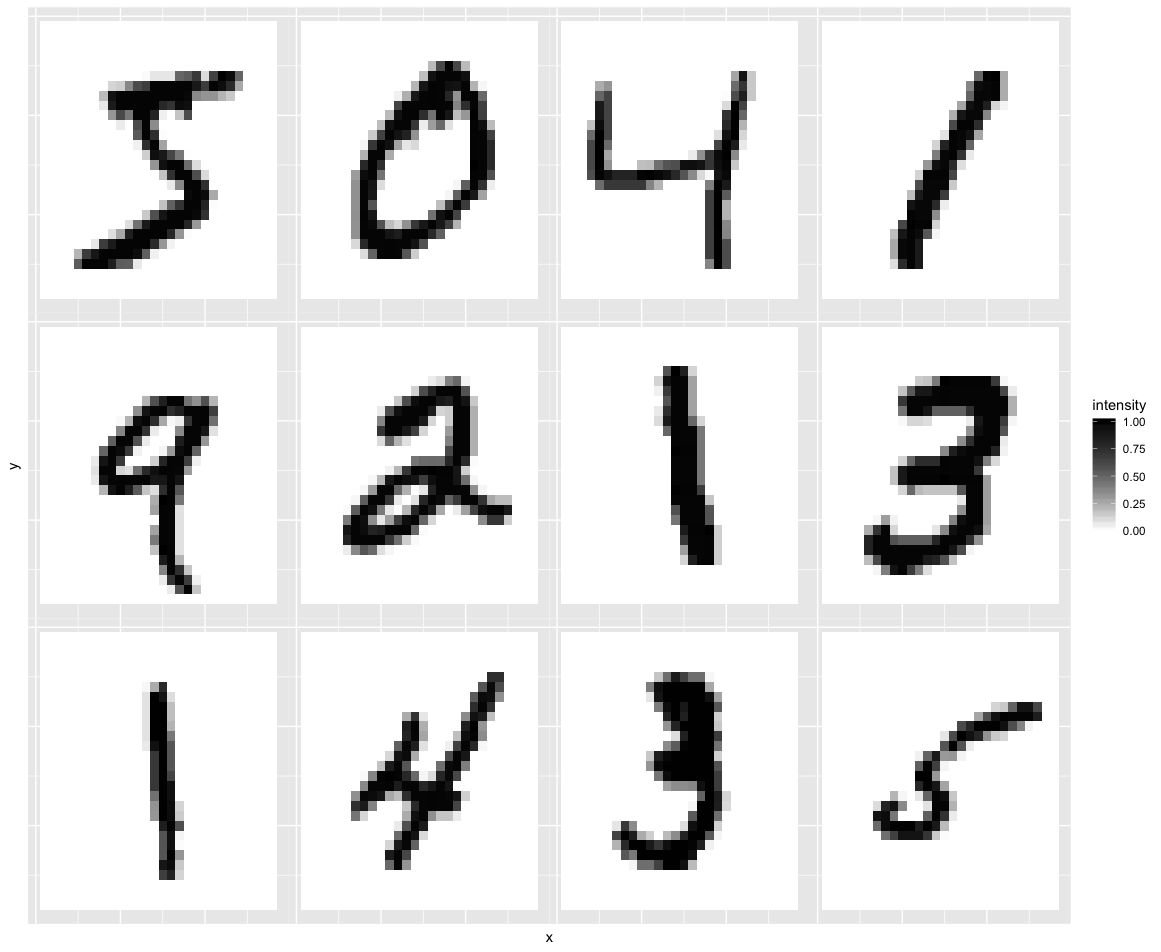
\includegraphics{MNIST2.png}

Each digit has been converted to a grid of \(28\times 28\) pixels, with a grayscale intensity level specified for each pixel. When we store these on a computer, we flatten each grid to a vector of length 784.
So for this dataset, \(n=60,000\) and \(p=784\). As an example of what the data look like, the intensities (times 100) for the first image above are shown in the plot below:

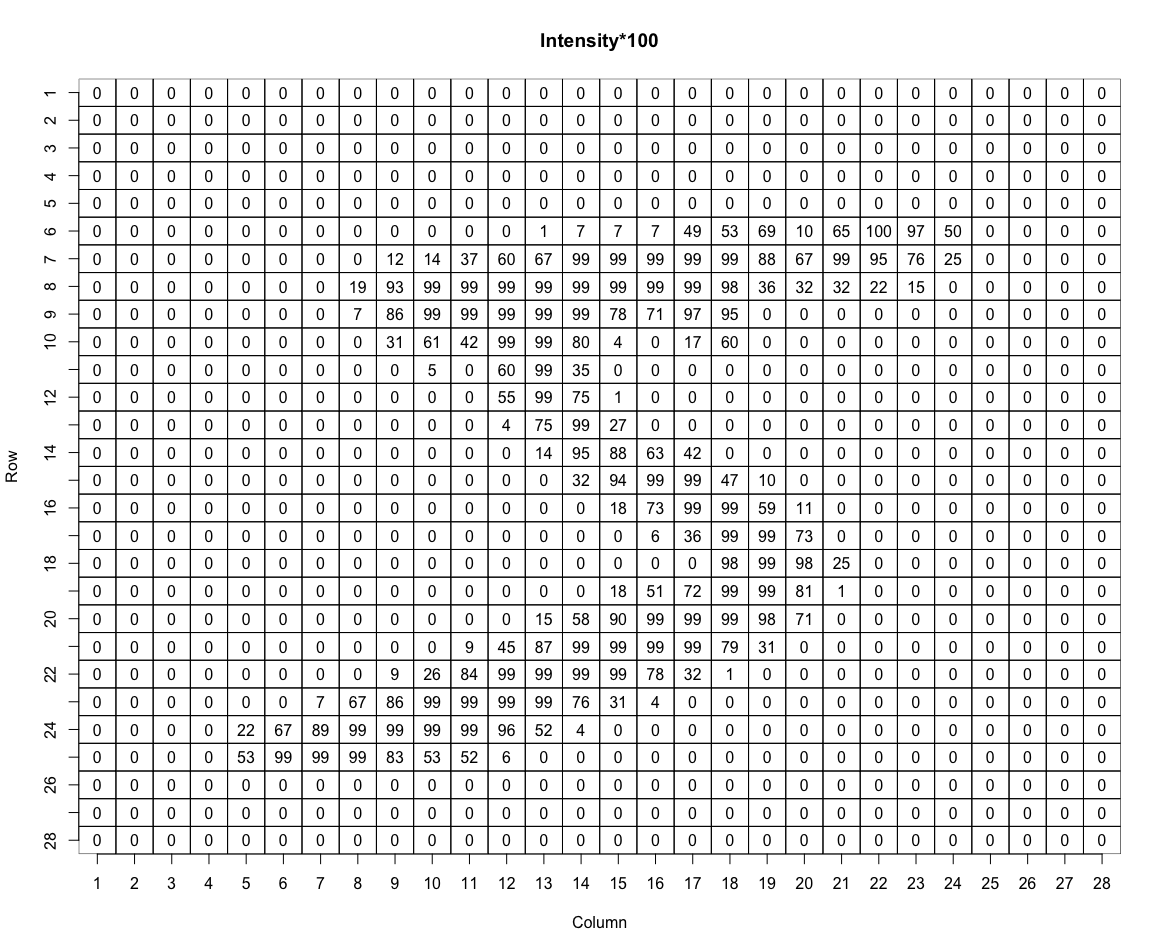
\includegraphics{MNIST3.png}
\end{example}

\hypertarget{aims-of-multivariate-data-analysis}{%
\subsection{Aims of multivariate data analysis}\label{aims-of-multivariate-data-analysis}}

The aim of multivariate statistical analysis is to answer questions such as:

\begin{itemize}
\tightlist
\item
  How can we visualise the data?
\item
  What is the joint distribution of marks?
\item
  Can we simplify the data? For example, we rank football teams using \(3W+D\) and we rank students by their average module mark. Is this fair? Can we reduce the dimension in a better way?
\item
  Can we use the data to discriminate, for example, between male and female students?
\item
  Are the different iris species different shapes?
\item
  Can we build a model to predict the intended digit from an image of someones handwriting? Or predict the species of iris from measurements of its sepal and petal?
\end{itemize}

We could just apply standard univariate techniques to each variable in turn, but this ignores possible dependencies between the variables which we must represent to draw valid conclusions.

\textbf{What is the difference between MVA and standard linear regression?}

\begin{itemize}
\tightlist
\item
  In standard linear regression we have a scalar response variable, \(y\) say, and a vector of covariates, \(\mathbf x\), say. The focus of interest is on how knowledge of \(\mathbf x\) influences the distribution of \(y\) (in particular, the mean of \(y\)). In contrast, in MVA the focus is a vector \(\mathbf y\), in which all the components of \(\mathbf y\) are viewed as responses rather than covariates, possibly with additional covariate information \(\mathbf x\). We will discuss this further in Chapter \ref{lm}.
\end{itemize}

\hypertarget{exploratory-data-analysis-eda}{%
\section{Exploratory data analysis (EDA)}\label{exploratory-data-analysis-eda}}

\begin{quote}
A picture is worth a thousand words
\end{quote}

\begin{figure}
\centering
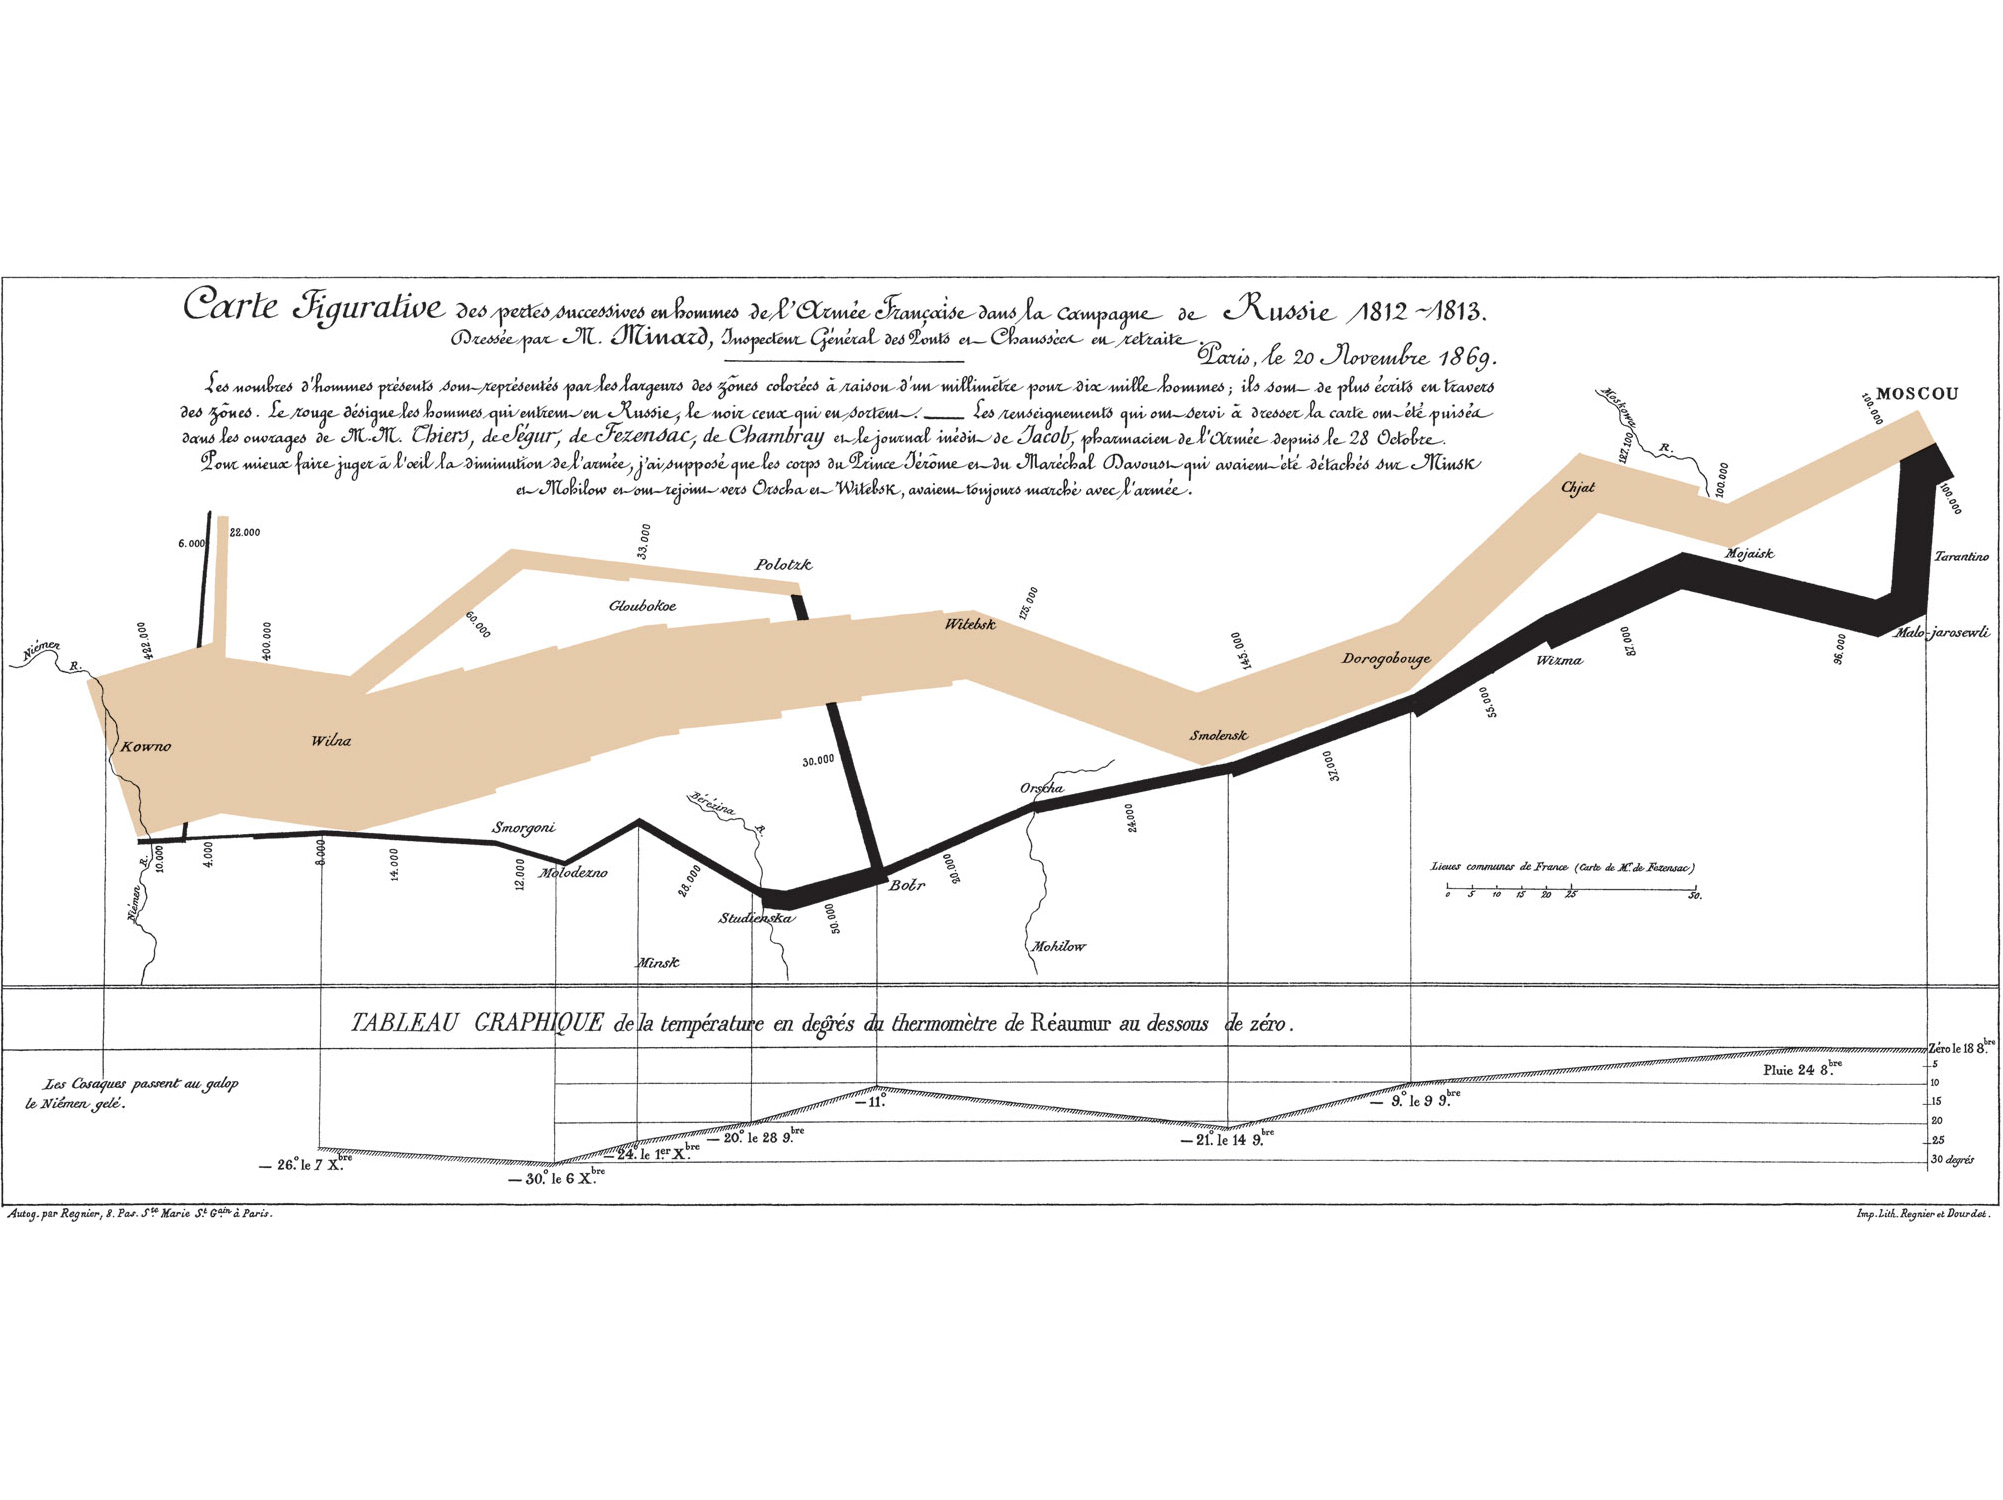
\includegraphics{figs/Minard.jpg}
\caption{\label{fig:unnamed-chunk-5}Charles Joseph Minard's famous map of Napoleon's 1812 invasion of Russian. It displays \href{https://en.wikipedia.org/wiki/Charles_Joseph_Minard\#The_map_of_Napoleon's_Russian_campaign}{six types of data in two dimensions}.}
\end{figure}

Before trying any form of statistical analysis, it is always a good idea to do some form of exploratory data analysis to understand the challenges presented by the data. As a minimum, this usually involves finding out whether each variable is continuous, discrete, or categorical, doing some basic visualization (plots), and perhaps computing a few summary statistics such as the mean and variance.

\hypertarget{data-visualization}{%
\subsection{Data visualization}\label{data-visualization}}

Visualising datasets before fitting any models can be extremely useful. It allows us to see obvious patterns and relationships,and may suggest a sensible form of analysis.
With multivariate data, finding the right kind of plot is not always simple, and many different approaches have been proposed.

When \(p=1\) or \(p=2\) we can simply draw histograms and scatter plots (respectively) to view the distribution. For \(p \geq 3\) the task is harder. One solution is a matrix of pair-wise scatter plots using the \texttt{pairs} command in R. The graph below shows the relationship between goals scored (F), goals against (A) and points (PT) for 20 teams during a recent Premiership season.

\begin{figure}
\centering
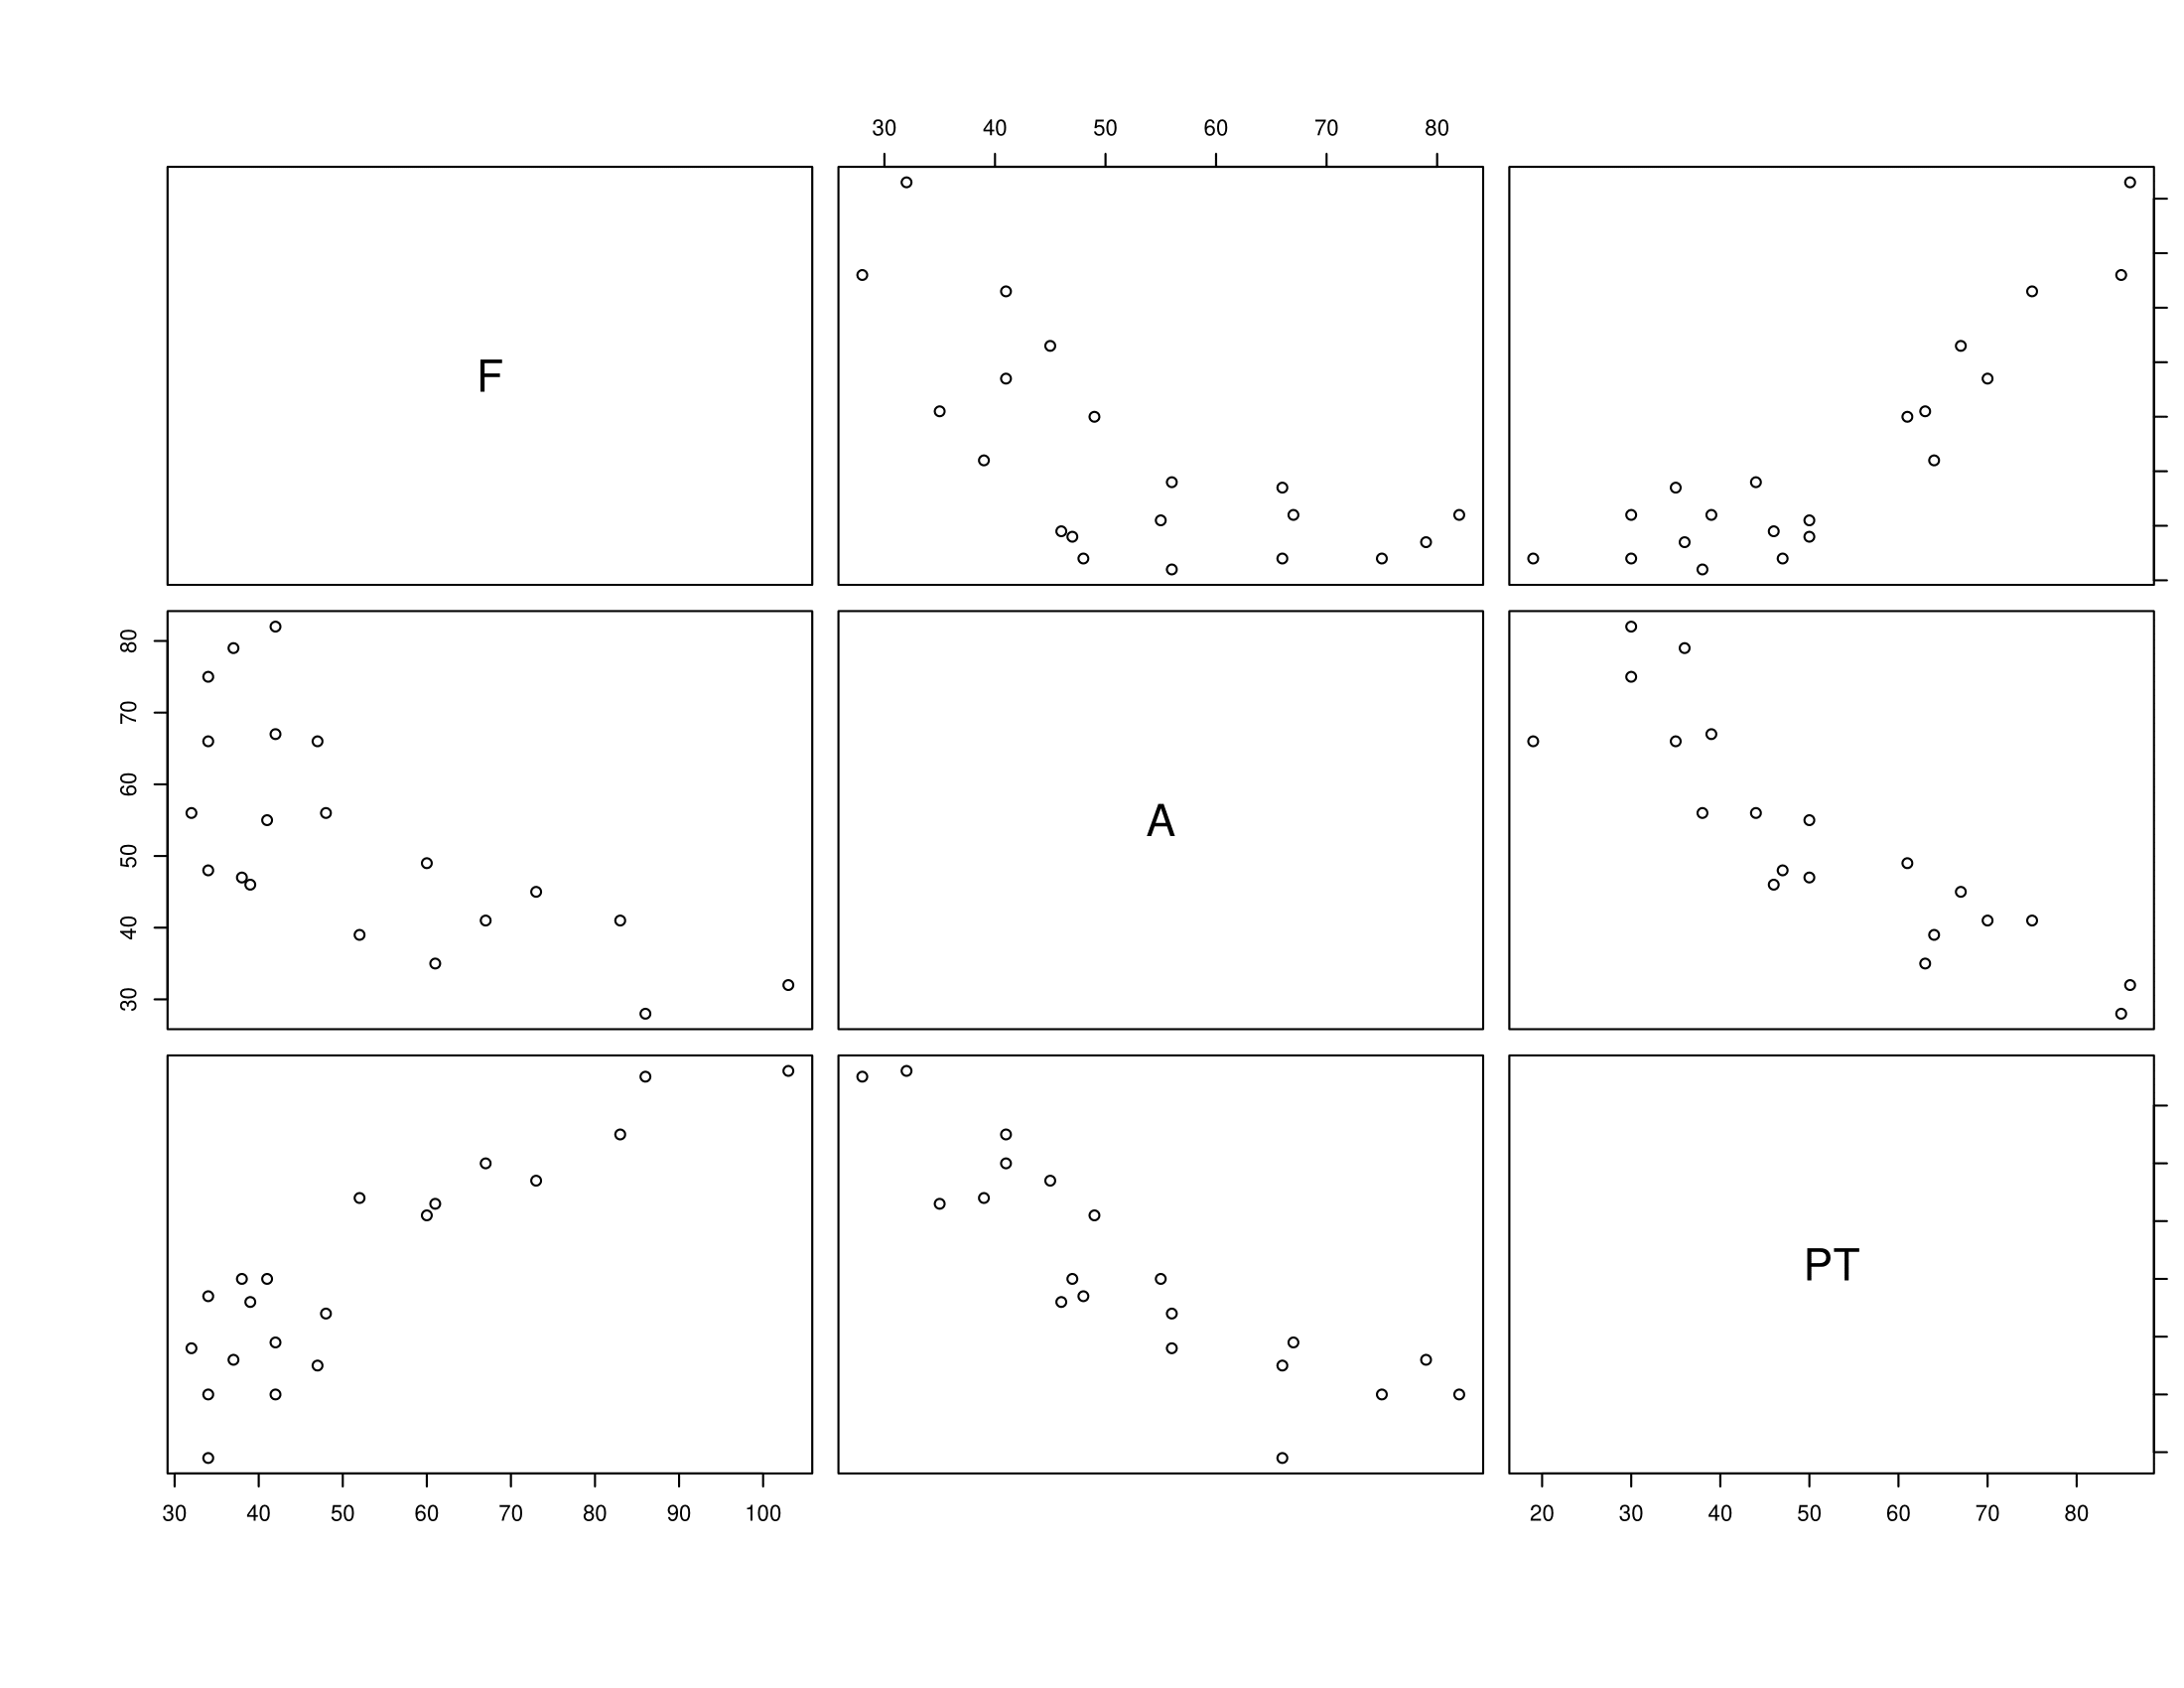
\includegraphics{figs/pairs.png}
\caption{\label{fig:unnamed-chunk-6}Scatter plots of goals for (F), goals against (A) and points (PT) for a recent Premier League Season}
\end{figure}

We can instantly see that points and goals scored are positively correlated, and that points and goals conceded (A) are negatively correlated (this is not a surprise of course).

R has a good basic plotting functionality. However, we will sometimes use packages that provide additional functionality. The first time you use a package you may need to install it. We can use \texttt{ggplot2} and \texttt{GGally} (which adds functionality to ggplot2) to add colour and detail to pairs plots. For example

\begin{Shaded}
\begin{Highlighting}[]
\KeywordTok{data}\NormalTok{(iris)}
\KeywordTok{library}\NormalTok{(ggplot2)}
\KeywordTok{library}\NormalTok{(GGally)}
\CommentTok{# pairs(iris) # - try the pairs command for comparison}
\KeywordTok{ggpairs}\NormalTok{(iris, }\DataTypeTok{columns=}\DecValTok{1}\OperatorTok{:}\DecValTok{4}\NormalTok{,  }\DataTypeTok{mapping=}\NormalTok{ggplot2}\OperatorTok{::}\KeywordTok{aes}\NormalTok{(}\DataTypeTok{colour =}\NormalTok{ Species),}
        \DataTypeTok{upper =} \KeywordTok{list}\NormalTok{(}\DataTypeTok{continuous =} \KeywordTok{wrap}\NormalTok{(}\StringTok{"cor"}\NormalTok{, }\DataTypeTok{size =} \DecValTok{3}\NormalTok{)))  }\CommentTok{# fix the font size}
\end{Highlighting}
\end{Shaded}

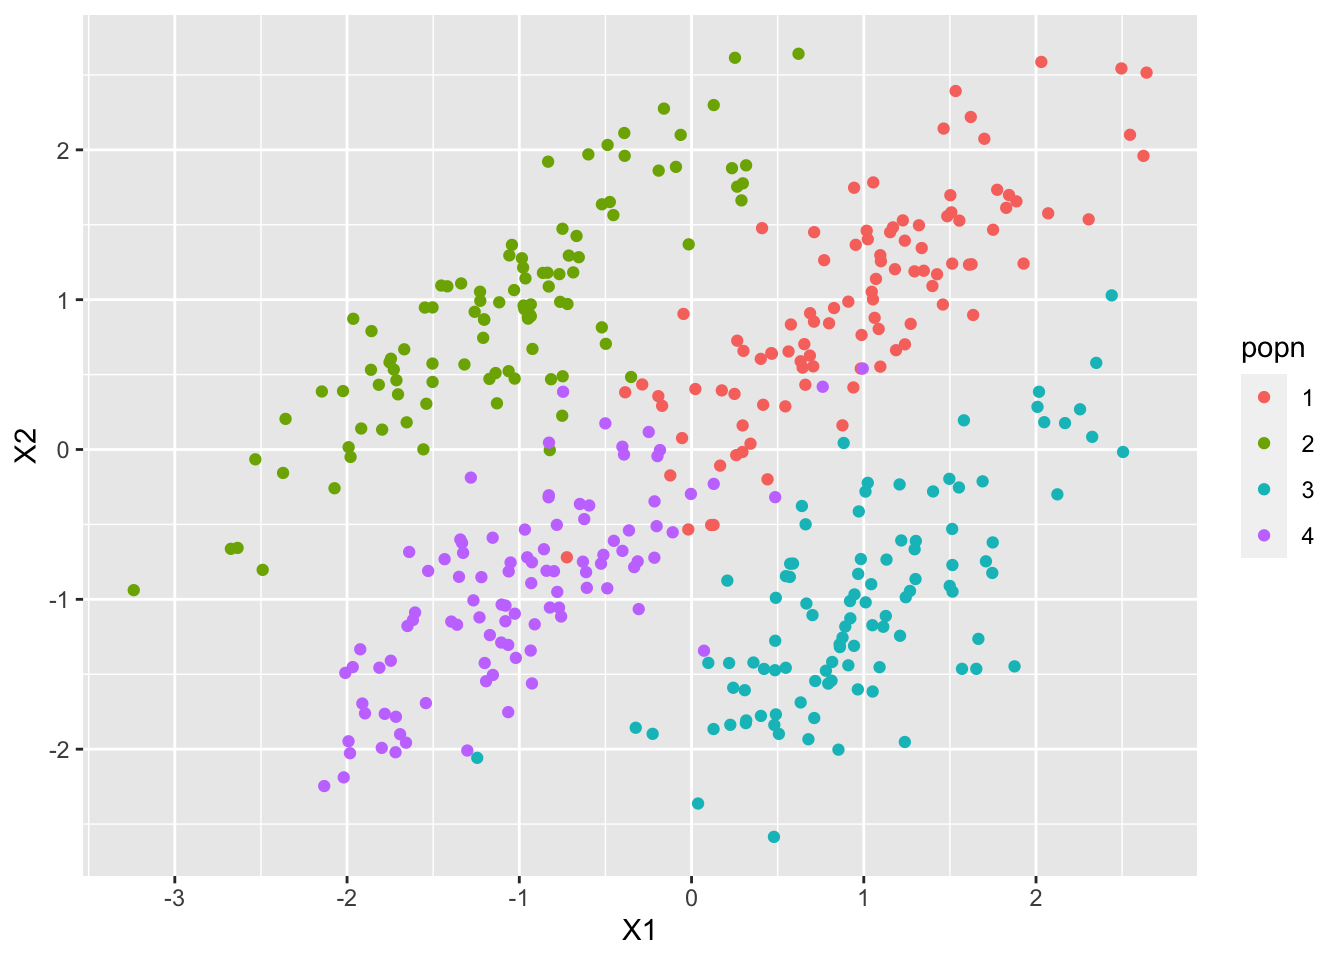
\includegraphics[width=1\linewidth]{01-statistical-prelim_files/figure-latex/unnamed-chunk-7-1}

This plot allows us to instantly see that there are clear differences between the three species of iris, at least when we look at the pairs plots. The benefit of adding colour in this case is that we can see the differences between the different species. Note how the sepal length and width are (weakly) negatively correlated across the entire dataset, but are positively correlated when we look at a single species at a time. We would have missed this information if we only used the \texttt{pairs} command (try it!).

Note that it is possible to miss key relationships when looking at \emph{marginals} plots such as these, as they only show two variables at a time. More complex relationships between three or more variables will not be visible. It is difficult visualize data in three or more dimensions. Many different types of plot have been proposed (e.g.~Google Chernoff faces). One approach is to use a \emph{parallel line} plot

\begin{Shaded}
\begin{Highlighting}[]
\KeywordTok{ggparcoord}\NormalTok{(iris, }\DecValTok{1}\OperatorTok{:}\DecValTok{4}\NormalTok{, }\DataTypeTok{groupColumn=}\DecValTok{5}\NormalTok{)}
\end{Highlighting}
\end{Shaded}

\includegraphics{01-statistical-prelim_files/figure-latex/unnamed-chunk-8-1.pdf}

Each case is represented by a single line, and here we have the information shown for the four continuous variables. The fifth variable \texttt{Species} is a discrete factor, and is shown by colouring the lines.

If you not familiar with \texttt{ggplot2}, a nice introduction can be found \href{https://ggplot2.tidyverse.org/}{here}. Details about `GGally can be found \href{https://ggobi.github.io/ggally/}{here}. A good way to see the variety of plots that are possible, and to find code to create them, is to browse plot galleries such as those available
\href{https://www.r-graph-gallery.com/ggplot2-package.html}{here}
and \href{https://www.data-to-viz.com}{here}.

\hypertarget{summary-statistics}{%
\subsection{Summary statistics}\label{summary-statistics}}

It is often useful to report a small number of numerical summaries of the data.
In univariate statistics we define the sample mean and sample variance of samples \(x_1, \ldots, x_n\) to be
\[ \bar{x} = \frac{1}{n} \sum_{i=1}^n x_i \quad \text{and} \quad s_{xx} = \frac{1}{n} \sum_{i=1}^n (x_i - \bar{x})^2 \]
and for two samples, \(x_1, \ldots, x_n\) and \(y_1, \ldots, y_n\), we define the sample covariance to be
\[s_{xy}=\frac{1}{n}\sum_{i=1}^n (x_i-\bar{x})(y_i-\bar{y}).\]

Analogous multivariate quantities can be defined as follows:

\begin{definition}
\protect\hypertarget{def:samplemean}{}{\label{def:samplemean} }For a sample of \(n\) points, each containing \(p\) variables, \(\mathbf x_1, \mathbf x_2, \ldots, \mathbf x_n \in \mathbb{R}^p\), the \textbf{sample mean} and \textbf{sample covariance matrix} are
\begin{align}
 \bar{\mathbf x} &= \frac{1}{n} \sum_{i=1}^n \mathbf x_i \label{eq:samplemean}\\
 \mathbf S&= \frac{1}{n} \sum_{i=1}^n (\mathbf x_i - \bar{\mathbf x}) (\mathbf x_i - \bar{\mathbf x})^\top 
\label{eq:samplecov}
\end{align}
where \(\mathbf x_i\in \mathbb{R}^p\) denotes the \(p\) variables observed on the \(i\)th subject.
\end{definition}

Note that

\begin{itemize}
\tightlist
\item
  \(\bar{\mathbf x} \in \mathbb{R}^p\). The \(j\)th entry in \(\bar{\mathbf x}\) is simply the (univariate) sample mean of the \(j\)th variable.
\item
  \(\mathbf S\in \mathbb{R}^{p\times p}\). Note that the \(ij^{th}\) entry of \(\mathbf S\) is \(s_{ij}\), the sample covariance between variable \(i\) and variable \(j\). The \(i^{th}\) diagonal element is the (univariate) sample variance of the \(i\)th variable.\\
\item
  \(\mathbf S\) is symmetric since \(s_{ij}=s_{ji}\).
\item
  an alternative formula for \(\mathbf S\) is
  \[\mathbf S= \frac{1}{n} \left(\sum_{i=1}^n \mathbf x_i \mathbf x_i^\top \right)- \bar{\mathbf x} \bar{\mathbf x}^\top.\]
\item
  We have divided by \(n\) rather than \(n-1\) here, which gives the maximum likelihood estimator of the variance, rather than the unbiased variance estimator that is often used.
\end{itemize}

\begin{definition}
\protect\hypertarget{def:samplecor}{}{\label{def:samplecor} }The \textbf{sample correlation matrix}, \(\mathbf R\), is the matrix with \(ij^{th}\) entry \(r_{ij}\) equal to the sample correlation between variables \(i\) and \(j\), that is
\[ r_{ij} = \frac{s_{ij}}{\sqrt{s_{ii}s_{jj}}}. \]
\end{definition}

Note that

\begin{itemize}
\tightlist
\item
  If \(\mathbf D= \text{diag}(\sqrt{s_{11}}, \dots, \sqrt{s_{pp}})\), then\\
  \[ \mathbf R= \mathbf D^{-1} \mathbf S\mathbf D^{-1} \]
\item
  \(\mathbf R\) is symmetric
\item
  the diagonal entries of \(\mathbf R\) are exactly 1 (each variable is perfectly correlated with itself)
\item
  \(|r_{ij}| \leq 1\) for all \(i, j\)
\end{itemize}

Note that if we change the unit of measurement for the \(\mathbf x_i\)'s then \(\mathbf S\) will change but \(\mathbf R\) will not.

\begin{definition}
\protect\hypertarget{def:totalvar}{}{\label{def:totalvar} }The \textbf{total variation} in a data set is usually measured by \(\text{tr}(\mathbf S)\) where \(\text{tr}()\) is the trace function that sums the diagonal elements of the matrix. That is,
\[\text{tr}(\mathbf S) = s_{11} + s_{22} + \ldots + s_{pp}.\]
In other words, it is the sum of the univariate variances of each of the \(p\) variables.
\end{definition}

\hypertarget{random-vectors-and-matrices}{%
\section{Random vectors and matrices}\label{random-vectors-and-matrices}}

\begin{definition}
\protect\hypertarget{def:popmean}{}{\label{def:popmean} }The \textbf{population mean vector} of the random vector \(\mathbf x\) is
\[{\boldsymbol{\mu}}= {\mathbb{E}}(\mathbf x).\]

The \textbf{population covariance matrix} of \(\mathbf x\) is
\[ \boldsymbol{\Sigma}= {\mathbb{V}\operatorname{ar}}(\mathbf x) = {\mathbb{E}}\left((\mathbf x-{\mathbb{E}}(\mathbf x))(\mathbf x-{\mathbb{E}}(\mathbf x))^\top \right).\]

The \textbf{covariance} between \(\mathbf x\) (\(p \times 1\)) and \(\mathbf y\) (\(q \times 1\)) is
\[ {\mathbb{C}\operatorname{ov}}(\mathbf x,\mathbf y) = {\mathbb{E}}\left((\mathbf x- {\mathbb{E}}(\mathbf x))(\mathbf y- {\mathbb{E}}(\mathbf y))^\top \right). \]
\end{definition}

Let \(\mathbf A\) denote a \(q \times p\) constant matrix, and let \(\mathbf b\) a constant vector of size \(q \times 1\).
Expectation is a linear operator in the sense that

\[{\mathbb{E}}(\mathbf A\mathbf x+ \mathbf b) = \mathbf A{\mathbb{E}}(\mathbf x) + \mathbf b=\mathbf A{\boldsymbol{\mu}}+\mathbf b.\]

The following properties follow:

\begin{itemize}
\tightlist
\item
  \({\mathbb{V}\operatorname{ar}}(\mathbf x) = {\mathbb{E}}(\mathbf x\mathbf x^\top) - {\boldsymbol{\mu}}{\boldsymbol{\mu}}^\top\).
\item
  \({\mathbb{V}\operatorname{ar}}(\mathbf A\mathbf x+ \mathbf b) = \mathbf A\boldsymbol{\Sigma}\mathbf A^\top\)
\item
  \({\mathbb{C}\operatorname{ov}}(\mathbf x,\mathbf y) = {\mathbb{E}}(\mathbf x\mathbf y^\top) - {\mathbb{E}}(\mathbf x) {\mathbb{E}}(\mathbf y)^\top\).
\item
  \({\mathbb{C}\operatorname{ov}}(\mathbf x,\mathbf x) = \boldsymbol{\Sigma}\).
\item
  \({\mathbb{C}\operatorname{ov}}(\mathbf x,\mathbf y) = {\mathbb{C}\operatorname{ov}}(\mathbf y,\mathbf x)^\top\).
\item
  \({\mathbb{C}\operatorname{ov}}(\mathbf A\mathbf x,\mathbf B\mathbf y) = \mathbf A{\mathbb{C}\operatorname{ov}}(\mathbf x,\mathbf y)\mathbf B^\top\)
\item
  If \(p=q\) then
  \[
  {\mathbb{V}\operatorname{ar}}(\mathbf x+ \mathbf y) = {\mathbb{V}\operatorname{ar}}(\mathbf x) + {\mathbb{V}\operatorname{ar}}(\mathbf y) + {\mathbb{C}\operatorname{ov}}(\mathbf x,\mathbf y) + {\mathbb{C}\operatorname{ov}}(\mathbf y,\mathbf x).
  \]
\end{itemize}

Finally, note that if \(\mathbf x\) and \(\mathbf y\) are independent (in which case I will write \(\mathbf x\perp \!\!\! \perp\mathbf y\)) then \({\mathbb{C}\operatorname{ov}}(\mathbf x,\mathbf y) = {\mathbf 0}_{p,q}\), i.e., a \(p\times q\) matrix of zeros.

\hypertarget{estimators}{%
\subsection{Estimators}\label{estimators}}

The population mean vector \({\boldsymbol{\mu}}\) and population covariance matrix \(\boldsymbol{\Sigma}\) will usually be unknown. We can use data to \textbf{estimate} these quantities.

\begin{itemize}
\tightlist
\item
  The sample mean \(\bar{\mathbf x}\) is often used as an estimator of \({\boldsymbol{\mu}}\).
\item
  The sample covariance matrix \(\mathbf S\) is often used as an estimator of \(\boldsymbol{\Sigma}\).
\end{itemize}

Equation \eqref{eq:samplemean} gives an unbiased estimator of the sample mean. The sample covariance matrix \eqref{eq:samplecov} is a biased estimator of the population covariance matrix. An unbiased estimate is obtained by dividing by \(n-1\) rather than \(n\) in Equation \eqref{eq:samplecov}.

\hypertarget{computer-tasks}{%
\section{Computer tasks}\label{computer-tasks}}

If you haven't done so already, please download and install R and Rstudio. R is the programming language, and Rstudio is an integrated development environment that makes using R much more pleasurable. My advice is to always use Rstudio and never run code in R itself.

\begin{enumerate}
\def\labelenumi{\arabic{enumi}.}
\setcounter{enumi}{-1}
\item
  \textbf{For complete beginners:} For those who are completely new to R (or those who want a refresher), I recommend working through an online tutorial. \href{https://www.statmethods.net/r-tutorial/index.html}{This} tutorial looks good, but contains more than you'll need.
\item
  \textbf{Warm-up:} The most important aspects of R to focus on for this module are

  \begin{itemize}
  \tightlist
  \item
    Basic plotting
  \item
    Manipulation of matrices and data frames.
  \end{itemize}

  Let's look at the \texttt{iris} dataset.

  \begin{itemize}
  \tightlist
  \item
    Can you plot the sepal length against the sepal width?
  \end{itemize}

  We'll now do some exercises on data manipulation. Note that there are several ways to do basic data manipulation in R. You can use base R commands or if you prefer, you can use the \href{https://dplyr.tidyverse.org/}{dplyr} commands which are part of the \texttt{tidyverse} packages.
  For example, to select columns, in base you can do:
\end{enumerate}

\begin{Shaded}
\begin{Highlighting}[]
\NormalTok{iris[,}\DecValTok{2}\NormalTok{] }\CommentTok{# selects column 2}
\NormalTok{iris}\OperatorTok{$}\NormalTok{Sepal.Width }\CommentTok{# selects the same column by name}
\end{Highlighting}
\end{Shaded}

or using dplyr you can do

\begin{Shaded}
\begin{Highlighting}[]
\KeywordTok{library}\NormalTok{(dplyr)}
\KeywordTok{select}\NormalTok{(iris, }\StringTok{"Sepal.Width"}\NormalTok{)}
\end{Highlighting}
\end{Shaded}

\begin{itemize}
\item
  Can you select the column of the \texttt{iris} data that contains just the sepal length and add it to the sepal width?

  To select only certain rows of the data (i.e.~to filter it), we can again use either base R or dplyr.
\end{itemize}

\begin{Shaded}
\begin{Highlighting}[]
\NormalTok{iris[iris[,}\DecValTok{3}\NormalTok{]}\OperatorTok{<}\DecValTok{5}\NormalTok{,] }\CommentTok{# select all rows that have a petal length less than 5.}
\KeywordTok{filter}\NormalTok{(iris, Petal.Length}\OperatorTok{<}\DecValTok{5}\NormalTok{) }\CommentTok{# do the same thing using dplyr}
\end{Highlighting}
\end{Shaded}

\begin{itemize}
\item
  Can you now select all the rows of the \texttt{iris} data frame that are for species \emph{setosa}? What is the mean petal length for these flowers?
\item
  Can you select all the flowers that have a sepal length greater than 5? What is the proportion of each species of iris in this set?
\end{itemize}

A nice aspect of dplyr is that you can chain commmands together. So for example, to select the versicolour flowers with petal width less than 1.5, we can do

\begin{Shaded}
\begin{Highlighting}[]
\NormalTok{iris }\OperatorTok\StringTok{ }\KeywordTok{filter}\NormalTok{(Species}\OperatorTok{==}\StringTok{'versicolor'}\NormalTok{) }\OperatorTok\StringTok{ }\KeywordTok{filter}\NormalTok{(Petal.Width}\OperatorTok{<}\FloatTok{1.5}\NormalTok{)}
\end{Highlighting}
\end{Shaded}

\begin{itemize}
\tightlist
\item
  Can you select all the flowers that have a sepal length greater than 6, and a petal length less than 5? What is the proportion of each species in this set?
\end{itemize}

Note that \texttt{iris} is a data frame

\begin{Shaded}
\begin{Highlighting}[]
\KeywordTok{is.data.frame}\NormalTok{(iris)}
\end{Highlighting}
\end{Shaded}

\begin{verbatim}
## [1] TRUE
\end{verbatim}

which is a type of structure used in R. This is convenient for some tasks, but not for others. Let's first extract the four numerical columns and store them as a matrix \(X\).

\begin{Shaded}
\begin{Highlighting}[]
\KeywordTok{is.matrix}\NormalTok{(iris)}
\end{Highlighting}
\end{Shaded}

\begin{verbatim}
## [1] FALSE
\end{verbatim}

\begin{Shaded}
\begin{Highlighting}[]
\NormalTok{X <-}\StringTok{ }\KeywordTok{as.matrix}\NormalTok{(iris[,}\DecValTok{1}\OperatorTok{:}\DecValTok{4}\NormalTok{])}
\KeywordTok{is.matrix}\NormalTok{(X)}
\end{Highlighting}
\end{Shaded}

\begin{verbatim}
## [1] TRUE
\end{verbatim}

\begin{itemize}
\tightlist
\item
  Select the 4 numerical columns and multiply the first column by 1, the second by 2, the third by 3, and the 4th by 4. One way to do this is by multiplying \(X\) by the diagonal matrix
\end{itemize}

\begin{Shaded}
\begin{Highlighting}[]
\KeywordTok{diag}\NormalTok{(}\DecValTok{1}\OperatorTok{:}\DecValTok{4}\NormalTok{)}
\end{Highlighting}
\end{Shaded}

\begin{verbatim}
##      [,1] [,2] [,3] [,4]
## [1,]    1    0    0    0
## [2,]    0    2    0    0
## [3,]    0    0    3    0
## [4,]    0    0    0    4
\end{verbatim}

\begin{enumerate}
\def\labelenumi{\arabic{enumi}.}
\setcounter{enumi}{1}
\tightlist
\item
  The table below shows the module marks for 5 students on the modules G11PRB (\(P\)) and G11STA (\(S\)).
\end{enumerate}

\begin{table}[H]
\centering
\begin{tabular}{lrr}
\toprule
Student & P & S\\
\midrule
A & 41 & 63\\
B & 72 & 82\\
C & 46 & 38\\
D & 77 & 57\\
E & 59 & 85\\
\bottomrule
\end{tabular}
\end{table}

\begin{itemize}
\tightlist
\item
  As an exercise, calculate the sample mean, sample covariance, sample correlation and total variation by hand.
\end{itemize}

\begin{itemize}
\tightlist
\item
  Now calculate these in R using \texttt{colMeans}, \texttt{cov}, and \texttt{cor}. These commands assume each column is a different variable, and each row a different observation.
\end{itemize}

\begin{Shaded}
\begin{Highlighting}[]
\KeywordTok{library}\NormalTok{(dplyr)}
\NormalTok{Ex1 <-}\StringTok{ }\KeywordTok{data.frame}\NormalTok{(}
  \DataTypeTok{Student=}\NormalTok{LETTERS[}\DecValTok{1}\OperatorTok{:}\DecValTok{5}\NormalTok{],}
  \DataTypeTok{P =} \KeywordTok{c}\NormalTok{(}\DecValTok{41}\NormalTok{,}\DecValTok{72}\NormalTok{,}\DecValTok{46}\NormalTok{,}\DecValTok{77}\NormalTok{,}\DecValTok{59}\NormalTok{),}
  \DataTypeTok{S =} \KeywordTok{c}\NormalTok{(}\DecValTok{63}\NormalTok{,}\DecValTok{82}\NormalTok{,}\DecValTok{38}\NormalTok{,}\DecValTok{57}\NormalTok{,}\DecValTok{85}\NormalTok{)}
\NormalTok{  )}

\NormalTok{Ex1 }\OperatorTok\StringTok{ }\KeywordTok{select_if}\NormalTok{(is.numeric) }\OperatorTok\StringTok{ }\NormalTok{colMeans}
\end{Highlighting}
\end{Shaded}

\begin{verbatim}
##  P  S 
## 59 65
\end{verbatim}

\begin{Shaded}
\begin{Highlighting}[]
\NormalTok{Ex1 }\OperatorTok\StringTok{ }\KeywordTok{select_if}\NormalTok{(is.numeric) }\OperatorTok\StringTok{ }\NormalTok{cov}
\end{Highlighting}
\end{Shaded}

\begin{verbatim}
##       P     S
## P 246.5 116.0
## S 116.0 371.5
\end{verbatim}

Note that by default R uses \(n-1\) in the denominator for the variance and covariance commands, whereas we used \(n\) in our definition.

We will be using the \texttt{dplyr} R package to perform basic data manipulation in R. If you are unfamiliar with \texttt{dplyr}, you can read about it at \url{https://dplyr.tidyverse.org/}. The pipe command \texttt{\%\textgreater{}\%} is particularly useful for chaining together multiple commands.

You could compute the same quantities using more familiar commands by selecting the numerical columns:

\begin{Shaded}
\begin{Highlighting}[]
\KeywordTok{colMeans}\NormalTok{(Ex1[,}\DecValTok{2}\OperatorTok{:}\DecValTok{3}\NormalTok{])}
\end{Highlighting}
\end{Shaded}

\begin{verbatim}
##  P  S 
## 59 65
\end{verbatim}

\begin{Shaded}
\begin{Highlighting}[]
\KeywordTok{cov}\NormalTok{(Ex1[,}\DecValTok{2}\OperatorTok{:}\DecValTok{3}\NormalTok{])}
\end{Highlighting}
\end{Shaded}

\begin{verbatim}
##       P     S
## P 246.5 116.0
## S 116.0 371.5
\end{verbatim}

\begin{itemize}
\tightlist
\item
  Can you compute the covariance matrix using the definition in Equation \eqref{eq:samplecov}?
\end{itemize}

\begin{enumerate}
\def\labelenumi{\arabic{enumi}.}
\setcounter{enumi}{2}
\tightlist
\item
  The \texttt{mtcars} dataset is another built-in dataset in R. You can read about it by typing \texttt{?mtcars} in R. Note that some of the variables are factors. You can ensure R treats them as factors by using the following command to create a dataset where they are listed as factors:
\end{enumerate}

\begin{Shaded}
\begin{Highlighting}[]
\NormalTok{mtcars2 <-}\StringTok{ }\KeywordTok{within}\NormalTok{(mtcars, \{}
\NormalTok{   vs <-}\StringTok{ }\KeywordTok{factor}\NormalTok{(vs, }\DataTypeTok{labels =} \KeywordTok{c}\NormalTok{(}\StringTok{"V"}\NormalTok{, }\StringTok{"S"}\NormalTok{))}
\NormalTok{   am <-}\StringTok{ }\KeywordTok{factor}\NormalTok{(am, }\DataTypeTok{labels =} \KeywordTok{c}\NormalTok{(}\StringTok{"automatic"}\NormalTok{, }\StringTok{"manual"}\NormalTok{))}
\NormalTok{   cyl  <-}\StringTok{ }\KeywordTok{ordered}\NormalTok{(cyl)}
\NormalTok{   gear <-}\StringTok{ }\KeywordTok{ordered}\NormalTok{(gear)}
\NormalTok{   carb <-}\StringTok{ }\KeywordTok{ordered}\NormalTok{(carb)}
\NormalTok{\})}
\end{Highlighting}
\end{Shaded}

\begin{verbatim}
Work with the `mtcars2` dataframe when you use `ggplot2`.
\end{verbatim}

\begin{itemize}
\tightlist
\item
  Create some plots to explore the structure of this dataset using ggplot2.
\item
  Try using the \texttt{pairs} command from base R and the \texttt{ggpairs} command from GGally.
\item
  Try colouring the scatter plots accoring to whether the car is automatic or not. - Create another plot using colour to represent the number of gears.
\item
  Find another type of plot from one of the plot galleries and try to create a similar plot with these data.
\end{itemize}

\begin{enumerate}
\def\labelenumi{\arabic{enumi}.}
\setcounter{enumi}{3}
\tightlist
\item
  We can 100 generate samples from the multivariate normal distribution with mean vector
  \[{\boldsymbol{\mu}}= \left(\begin{array}{c}1\\0\end{array}\right)\]
  and covariance matrix
  \[\boldsymbol{\Sigma}= \left(\begin{array}{cc}2&1\\1&2\end{array}\right)\]
  as follows (you may need to install the R package \texttt{mvtnorm} first):
\end{enumerate}

\begin{Shaded}
\begin{Highlighting}[]
\KeywordTok{library}\NormalTok{(mvtnorm)}
\NormalTok{mu =}\StringTok{ }\KeywordTok{c}\NormalTok{(}\DecValTok{1}\NormalTok{,}\DecValTok{0}\NormalTok{)}
\NormalTok{Sigma=}\KeywordTok{matrix}\NormalTok{(}\KeywordTok{c}\NormalTok{(}\DecValTok{2}\NormalTok{,}\DecValTok{1}\NormalTok{,}\DecValTok{1}\NormalTok{,}\DecValTok{2}\NormalTok{), }\DataTypeTok{nr=}\DecValTok{2}\NormalTok{)}
\NormalTok{X <-}\StringTok{ }\KeywordTok{rmvnorm}\NormalTok{(}\DataTypeTok{n=}\DecValTok{100}\NormalTok{, }\DataTypeTok{mean=}\NormalTok{mu, }\DataTypeTok{sigma=}\NormalTok{Sigma)}
\end{Highlighting}
\end{Shaded}

\begin{itemize}
\tightlist
\item
  Compute the sample mean and covariance matrix of these samples.
\item
  Generate a new sample dataset, \(X\), and recompute the sample mean and covariance matrix. What do you notice?
\item
  Try changing \(n\), the number of samples (making it much larger say), and now recomputing the mean and covariance. What do you notice?
\end{itemize}

\begin{enumerate}
\def\labelenumi{\arabic{enumi}.}
\setcounter{enumi}{4}
\tightlist
\item
  \textbf{Optional} Download the MNIST data from Moodle and load it into R.
\end{enumerate}

\begin{Shaded}
\begin{Highlighting}[]
\KeywordTok{load}\NormalTok{(}\StringTok{'mnist.rda'}\NormalTok{)}
\end{Highlighting}
\end{Shaded}

This loads a list \texttt{mnist} that splits the data into two parts

\begin{Shaded}
\begin{Highlighting}[]
\NormalTok{mnist}\OperatorTok{$}\NormalTok{train }\CommentTok{## a training set of 60000 images}
\NormalTok{mnist}\OperatorTok{$}\NormalTok{test }\CommentTok{## a test set of 10000 images}
\end{Highlighting}
\end{Shaded}

Let's just look at the training set. This is also a list containing the image intensities and the image labels

\begin{Shaded}
\begin{Highlighting}[]
\NormalTok{mnist}\OperatorTok{$}\NormalTok{train}\OperatorTok{$}\NormalTok{x }\CommentTok{# image intensities}
\NormalTok{mnist}\OperatorTok{$}\NormalTok{train}\OperatorTok{$}\NormalTok{y }\CommentTok{# image labels}
\end{Highlighting}
\end{Shaded}

If we select just the first image we can see it is a vector of length 784 containing numbers between 0 and 1.

\begin{Shaded}
\begin{Highlighting}[]
\NormalTok{mnist}\OperatorTok{$}\NormalTok{train}\OperatorTok{$}\NormalTok{x[}\DecValTok{1}\NormalTok{,]}
\end{Highlighting}
\end{Shaded}

I've created a function to help you plot these images.

\begin{Shaded}
\begin{Highlighting}[]
\KeywordTok{library}\NormalTok{(reshape2)}
\KeywordTok{library}\NormalTok{(ggplot2)}


\NormalTok{plot.mnist <-}\StringTok{ }\ControlFlowTok{function}\NormalTok{(im)\{}
  \CommentTok{#im[im<0]<-0 # set any negative intensities to zero}
  \CommentTok{#im[im>1]<-1 # set an intensities bigger than 1 to 1.}
  
  
  \ControlFlowTok{if}\NormalTok{(}\KeywordTok{is.vector}\NormalTok{(im))\{ }\CommentTok{# a single image}
    
\NormalTok{    A<-}\KeywordTok{matrix}\NormalTok{(im, }\DataTypeTok{nr=}\DecValTok{28}\NormalTok{, }\DataTypeTok{byrow=}\NormalTok{F)}
\NormalTok{    C<-}\StringTok{ }\KeywordTok{melt}\NormalTok{(A, }\DataTypeTok{varnames =} \KeywordTok{c}\NormalTok{(}\StringTok{"x"}\NormalTok{, }\StringTok{"y"}\NormalTok{), }\DataTypeTok{value.name =} \StringTok{"intensity"}\NormalTok{)}
\NormalTok{    p<-}\KeywordTok{ggplot}\NormalTok{(C, }\KeywordTok{aes}\NormalTok{(}\DataTypeTok{x =}\NormalTok{ x, }\DataTypeTok{y =}\NormalTok{ y, }\DataTypeTok{fill =}\NormalTok{ intensity))}\OperatorTok{+}
\StringTok{      }\KeywordTok{geom_tile}\NormalTok{(}\KeywordTok{aes}\NormalTok{(}\DataTypeTok{fill=}\NormalTok{intensity))}\OperatorTok{+}
\StringTok{      }\KeywordTok{scale_fill_gradient}\NormalTok{(}\DataTypeTok{low=}\StringTok{'white'}\NormalTok{, }\DataTypeTok{high=}\StringTok{'black'}\NormalTok{)}\OperatorTok{+}
\StringTok{      }\KeywordTok{scale_y_reverse}\NormalTok{()}\OperatorTok{+}\KeywordTok{theme}\NormalTok{(}
        \DataTypeTok{strip.background =} \KeywordTok{element_blank}\NormalTok{(),}
        \DataTypeTok{strip.text.x =} \KeywordTok{element_blank}\NormalTok{(),}
        \DataTypeTok{panel.spacing =} \KeywordTok{unit}\NormalTok{(}\DecValTok{0}\NormalTok{, }\StringTok{"lines"}\NormalTok{),}
        \DataTypeTok{axis.text =} \KeywordTok{element_blank}\NormalTok{(),}
        \DataTypeTok{axis.ticks =} \KeywordTok{element_blank}\NormalTok{()}
\NormalTok{      ) }
\NormalTok{  \}}
  \ControlFlowTok{else}\NormalTok{\{}
    \ControlFlowTok{if}\NormalTok{ (}\KeywordTok{dim}\NormalTok{(im)[}\DecValTok{2}\NormalTok{]}\OperatorTok{!=}\DecValTok{784}\NormalTok{)\{}
\NormalTok{      im =}\StringTok{ }\KeywordTok{t}\NormalTok{(im)}
\NormalTok{    \} }
\NormalTok{    n <-}\StringTok{ }\KeywordTok{dim}\NormalTok{(im)[}\DecValTok{1}\NormalTok{]}
\NormalTok{    As <-}\StringTok{ }\KeywordTok{array}\NormalTok{(im, }\DataTypeTok{dim =} \KeywordTok{c}\NormalTok{(n, }\DecValTok{28}\NormalTok{, }\DecValTok{28}\NormalTok{))}
    
\NormalTok{    Cs<-}\StringTok{ }\KeywordTok{melt}\NormalTok{(As, }\DataTypeTok{varnames =} \KeywordTok{c}\NormalTok{(}\StringTok{"image"}\NormalTok{,}\StringTok{"x"}\NormalTok{, }\StringTok{"y"}\NormalTok{), }\DataTypeTok{value.name =} \StringTok{"intensity"}\NormalTok{)}
\NormalTok{    p<-}\KeywordTok{ggplot}\NormalTok{(Cs, }\KeywordTok{aes}\NormalTok{(}\DataTypeTok{x =}\NormalTok{ x, }\DataTypeTok{y =}\NormalTok{ y, }\DataTypeTok{fill =}\NormalTok{ intensity))}\OperatorTok{+}
\StringTok{      }\KeywordTok{geom_tile}\NormalTok{(}\KeywordTok{aes}\NormalTok{(}\DataTypeTok{fill=}\NormalTok{intensity))}\OperatorTok{+}
\StringTok{      }\KeywordTok{scale_fill_gradient}\NormalTok{(}\DataTypeTok{low=}\StringTok{'white'}\NormalTok{, }\DataTypeTok{high=}\StringTok{'black'}\NormalTok{)}\OperatorTok{+}
\StringTok{      }\KeywordTok{facet_wrap}\NormalTok{(}\OperatorTok{~}\StringTok{ }\NormalTok{image, }\DataTypeTok{nrow =} \KeywordTok{floor}\NormalTok{(}\KeywordTok{sqrt}\NormalTok{(n))}\OperatorTok{+}\DecValTok{1}\NormalTok{, }\DataTypeTok{ncol =} \KeywordTok{floor}\NormalTok{(}\KeywordTok{sqrt}\NormalTok{(n))}\OperatorTok{+}\DecValTok{1}\NormalTok{)}\OperatorTok{+}
\StringTok{      }\KeywordTok{scale_y_reverse}\NormalTok{()}\OperatorTok{+}\KeywordTok{theme}\NormalTok{(}
        \DataTypeTok{strip.background =} \KeywordTok{element_blank}\NormalTok{(),}
        \DataTypeTok{strip.text.x =} \KeywordTok{element_blank}\NormalTok{(),}
        \DataTypeTok{panel.spacing =} \KeywordTok{unit}\NormalTok{(}\DecValTok{0}\NormalTok{, }\StringTok{"lines"}\NormalTok{),}
        \DataTypeTok{axis.text =} \KeywordTok{element_blank}\NormalTok{(),}
        \DataTypeTok{axis.ticks =} \KeywordTok{element_blank}\NormalTok{()}
\NormalTok{      ) }
    
\NormalTok{  \}}
  \KeywordTok{return}\NormalTok{(p)}
\NormalTok{\}}
\end{Highlighting}
\end{Shaded}

\begin{itemize}
\item
  Use this command to plot the first 10 images from the MNIST training set.
\item
  Select all the 5s from the MNIST training set. Plot a selection of these digits.
\end{itemize}

\hypertarget{exercises}{%
\section{Exercises}\label{exercises}}

\begin{enumerate}
\def\labelenumi{\arabic{enumi}.}
\item
  Show that the two formulae for the population covariance matrix \(\boldsymbol{\Sigma}\) are equivalent, i.e.~show that
  \[\boldsymbol{\Sigma}= {\mathbb{E}}[(\mathbf x- {\boldsymbol{\mu}}) (\mathbf x- {\boldsymbol{\mu}})^\top ] = {\mathbb{E}}[ \mathbf x\mathbf x^\top ] - {\boldsymbol{\mu}}{\boldsymbol{\mu}}^\top.\]
\item
  Let \(\mathbf x_1, \ldots, \mathbf x_n\) be a \(p\)-dimensional sample with mean \(\bar{\mathbf x}\) and sample covariance matrix \(\mathbf S\). Consider the transformation \(\mathbf y_i = \mathbf A\mathbf x_i + \mathbf c\) where \(\mathbf A\) is a fixed \(q \times p\) matrix and \(\mathbf c\) is a fixed \(q\)-dimensional vector. Let \(\mathbf T\) be the sample covariance matrix of \(\mathbf y_1, \ldots, \mathbf y_n\). Show
\end{enumerate}

\begin{itemize}
\item
  \(\bar{\mathbf y} = \mathbf A\bar{\mathbf x} + \mathbf c\),
\item
  \(\mathbf T= \mathbf A\mathbf S\mathbf A^\top\).

  Assuming now that \(\mathbf x\) is a random vector with \({\mathbb{E}}(\mathbf x)={\boldsymbol{\mu}}\), \({\mathbb{V}\operatorname{ar}}(\mathbf x)=\boldsymbol{\Sigma}\), \(\mathbf y=\mathbf A\mathbf x+\mathbf c\) with \(\mathbf A\) and \(\mathbf c\) as before, \({\mathbb{E}}(\mathbf y)={\pmb \phi}\) and \({\mathbb{V}\operatorname{ar}}(\mathbf y)={\pmb \Omega}\), what are the population analogues of the results above?
\end{itemize}

\begin{enumerate}
\def\labelenumi{\arabic{enumi}.}
\setcounter{enumi}{2}
\item
  A sample of size \(n=144\) produced the following summary statistics
  \[ \sum_{i=1}^n \mathbf x_i = \begin{pmatrix} 392.2 \\ 1530.8 \end{pmatrix} \qquad \sum_{i=1}^n \mathbf x_i \mathbf x_i^\top = \begin{pmatrix} 1101.88 & 4305.17 \\ 4305.17 & 17120.88 \end{pmatrix}.\]
  Calculate the sample mean, the sample covariance matrix and the sample correlation coefficient.
\item
  Let \(\mathbf x\) and \(\mathbf y\) be independent random \(p\)-dimensional vectors. Assuming that all relevant moments exist, show that for any real scalars \(\alpha\) and \(\beta\),
  \[{\mathbb{V}\operatorname{ar}}(\alpha \mathbf x+ \beta \mathbf y) = \alpha^2 {\mathbb{V}\operatorname{ar}}(\mathbf x) + \beta^2 {\mathbb{V}\operatorname{ar}}(\mathbf y).\]

  What is the corresponding formula when \(\mathbf x\) and \(\mathbf y\) are not independent? Express your answer in terms of \({\mathbb{V}\operatorname{ar}}(\mathbf x)\), \({\mathbb{V}\operatorname{ar}}(\mathbf y)\) and \({\mathbb{C}\operatorname{ov}}(\mathbf x, \mathbf y)\).
\end{enumerate}

\hypertarget{linalg-prelim}{%
\chapter{Review of linear algebra}\label{linalg-prelim}}

Modern statistics and machine learning rely heavily upon linear algebra, nowhere more so than in multivariate statistics. In the first part of this chapter (sections \ref{linalg-basics} and \ref{linalg-vecspaces}) we review some concepts from linear algebra that will be needed throughout the module, including vector spaces, row and column spaces, the rank of a matrix, etc. Hopefully most of this will be familiar to you.

We then cover some basic details on inner-product or normed spaces in \ref{linalg-innerprod}, which are vector spaces equipped with a concept of distance and angle.
Finally, in Section \ref{centering-matrix} we will describe the centering matrix. Further details and proofs for this section will be tackled in the exercises in Section \ref{exercises-ch2}.

I do not provide proofs for many of the results stated in this chapter, but instead prove a small selection which I think it is useful to see. For a complete treatment of the linear algebra needed for this module, see the excellent book ``Linear algebra and learning from data'' by Gilbert Strang.

I have recorded videos on some (but not all) of the topics in these notes:

\begin{itemize}
\tightlist
\item
  \href{https://mediaspace.nottingham.ac.uk/media/Vector+Spaces/1_48xqrp04}{Vector spaces}
\item
  \href{https://mediaspace.nottingham.ac.uk/media/Matrices/1_nqo2u7zs}{Matrices}
\item
  \href{https://mediaspace.nottingham.ac.uk/media/Inner+Product+Spaces/1_nhcbybg3}{Inner product spaces}
\item
  \href{https://mediaspace.nottingham.ac.uk/media/Orthogonal+Matrices/1_rr2ervcs}{Orthogonal matrices}
\item
  \href{https://mediaspace.nottingham.ac.uk/media/Projection/1_soh726fg}{Projection matrices}
\end{itemize}

\hypertarget{linalg-basics}{%
\section{Basics}\label{linalg-basics}}

In this section, we recap some basic definitions and notation. Hopefully this material will largely be familiar to you.

\hypertarget{notation-1}{%
\subsection{Notation}\label{notation-1}}

The matrix \({\mathbf A}\) will be referred to in the following equivalent ways:
\begin{eqnarray*}
{\mathbf A}=\stackrel{n\times p}{\mathbf A} &=& \left(\begin{array}{cccc}
a_{11}&a_{12}&\dots&a_{1p}\\
a_{21}&a_{22}&\dots&a_{2p}\\
\vdots&\vdots&&\vdots\\
a_{n1}&a_{n2}&\dots&a_{np}
\end{array} \right) \\
&=&[a_{ij}: i=1, \ldots , n; j=1, \ldots , p]\\
&=&(a_{ij})\\
&=& \left( \begin{array}{c}\mathbf a_1^\top\\
\vdots\\
\mathbf a_n^\top\end{array}\right)
\end{eqnarray*}
where the \(a_{ij}\) are the individual entries, and \(\mathbf a_i^\top=(a_{i1}, a_{i2}, \ldots, a_{ip})\) is the \(i^{th}\) row.

A matrix of order \(1\times 1\) is called a \emph{scalar}.

A matrix of order \(n\times 1\) is called a \emph{(column) vector}.

A matrix of order \(1\times p\) is called a \emph{(row) vector}.

e.g. \(\stackrel{n\times 1}{\mathbf a}=\left( \begin{array}{c} a_1\\\vdots\\a_n \end{array} \right)\)\quad is a column vector.

The \(n\times n\) \emph{identity matrix} \({\mathbf I}_n\) has diagonal elements equal to 1
and off-diagonal elements equal to zero.

A \emph{diagonal} matrix is an \(n \times n\) matrix whose
off-diagonal elements are zero. Sometimes we denote a diagonal
matrix by \(\text{diag}\{a_1,\ldots, a_n\}\).

\[\mathbf I_3 = \left(\begin{array}{ccc} 1&0&0\\ 0&1&0\\ 0&0&1\end{array}\right),\quad \text{diag}\{1,2,3\}=\left(\begin{array}{ccc} 1&0&0\\ 0&2&0\\ 0&0&3\end{array}\right)\quad\]

\hypertarget{elementary-matrix-operations}{%
\subsection{Elementary matrix operations}\label{elementary-matrix-operations}}

\begin{enumerate}
\def\labelenumi{\arabic{enumi}.}
\item
  \emph{Addition/Subtraction}. If \(\stackrel{n\times p}{\mathbf A}=[a_{ij}]\) and \(\stackrel{n\times p}{\mathbf B}=[b_{ij}]\) are
  given matrices then
  \[ {\mathbf A}+{\mathbf B}=[a_{ij}+b_{ij}] \qquad \text{and} \qquad {\mathbf A}-{\mathbf B}=[a_{ij}-b_{ij}].\]
\item
  \emph{Scalar Multiplication}. If \(\lambda\) is a scalar and \({\mathbf A}=[a_{ij}]\) then
  \[\lambda {\mathbf A}=[\lambda a_{ij}].\]
\item
  \emph{Matrix Multiplication}. If \(\stackrel{n\times p}{\mathbf A}\) and \(\stackrel{p\times q}{\mathbf B}\) are
  matrices then \(\mathbf A\mathbf B=\stackrel{n\times q}{\mathbf C}=[c_{ij}]\) where
  \[c_{ij}=\sum _{k=1}^p a_{ik}b_{kj}, \qquad i=1,\dots,n, \qquad j=1,\dots ,q.\]
\item
  \emph{Matrix Transpose}. If \(\stackrel{m \times n}{\mathbf A}=[a_{ij}: i=1, \ldots , m; j=1, \ldots , n]\), then the transpose of \(\mathbf A\), written
  \(\mathbf A^\top\), is given by the \(n \times m\) matrix
  \[
  \mathbf A^\top =[a_{ji}: j=1, \ldots , n; i=1, \ldots, m].
  \]
  Note from the definitions that \((\mathbf A\mathbf B)^\top={\mathbf B}^\top {\mathbf A}^\top\).
\item
  \emph{Matrix Inverse}. The inverse of a matrix \(\stackrel{n\times n}{\mathbf A}\) (if it exists) is a
  matrix \(\stackrel{n\times n}{\mathbf B}\) such that \({\mathbf A}\mathbf B=\mathbf B\mathbf A={\mathbf I}_n.\) We denote
  the inverse by \({\mathbf A}^{-1}\). Note that if \({\mathbf A}_1\) and \({\mathbf A}_2\) are both invertible,
  then \(({\mathbf A}_1 {\mathbf A}_2)^{-1}={\mathbf A}_2^{-1}{\mathbf A}_1^{-1}\).
\item
  \emph{Trace}. The trace of a matrix \(\stackrel{n\times n}{\mathbf A}\) is given by
  \[ \text{tr}({\mathbf A})=\sum _{i=1}^n a_{ii}.\]
\end{enumerate}

\begin{lemma}
\protect\hypertarget{lem:trace}{}{\label{lem:trace} }For any matrices \(\mathbf A\) (\(n \times m\)) and \(\mathbf B\) (\(m \times n\)),
\[
\text{tr}(\mathbf A\mathbf B) = \text{tr}(\mathbf B\mathbf A).
\]
\end{lemma}

\begin{enumerate}
\def\labelenumi{\arabic{enumi}.}
\setcounter{enumi}{6}
\tightlist
\item
  The \emph{determinant} of a square matrix \(\stackrel{n\times n}{\mathbf A}\) is
  defined as
  \[ \text{det}({\mathbf A})=\sum (-1)^{|\tau |} a_{1\tau(1)}\dots a_{n\tau (n)} \]
  where the summation is taken over all permutations \(\tau\) of \(\{1,2,\dots ,n\}\),
  and we define \(|\tau |=0\) or \(1\) depending on whether \(\tau\) can be written as an even or
  odd number of transpositions.
\end{enumerate}

E.g. If \({\mathbf A}=\left[ \begin{array}{cc} a_{11}&a_{12}\\ a_{21}&a_{22} \end{array} \right]\),
then \(\text{det}({\mathbf A})=a_{11}a_{22}-a_{12}a_{21}\).

\begin{proposition}
\protect\hypertarget{prp:det1}{}{\label{prp:det1} }Matrix \(\stackrel{n\times n}{\mathbf A}\) is invertible if and only if \(\det(\mathbf A)\not = 0\). If \(\mathbf A^{-1}\) exists then
\[\det(\mathbf A)=\frac{1}{\det(\mathbf A^{-1})}\]
\end{proposition}

\begin{proposition}
\protect\hypertarget{prp:det3}{}{\label{prp:det3} }For any matrices \(\stackrel{n\times n}{\mathbf A}\),
\(\stackrel{n\times n}{\mathbf B}\), \(\stackrel{n\times n}{\mathbf C}\) such that \({\mathbf C}={\mathbf{AB}}\),
\[ \text{det}({\mathbf C})=\text{det}({\mathbf A}) \cdot \text{det}({\mathbf B}).\]
\end{proposition}

\hypertarget{special-matrices}{%
\subsection{Special matrices}\label{special-matrices}}

\begin{definition}
\protect\hypertarget{def:posdef}{}{\label{def:posdef} }An \(n\times n\) matrix \(\mathbf A\) is symmetric if
\[\mathbf A= \mathbf A^\top.\]
An \(n\times n\) symmetric matrix \(\mathbf A\) is \textbf{positive-definite} if
\[\mathbf x^\top \mathbf A\mathbf x>0 \mbox{ for all } \mathbf x\in \mathbb{R}^n, \mathbf x\not = \boldsymbol 0\]
and is \textbf{positive semi-definite} if
\[\mathbf x^\top \mathbf A\mathbf x\geq 0 \mbox{ for all } \mathbf x\in \mathbb{R}^n.\]

\(\mathbf A\) is \textbf{idempotent} if \(\mathbf A^2=\mathbf A\).
\end{definition}

\hypertarget{vectordiff}{%
\subsection{Vector Differentiation}\label{vectordiff}}

Consider a real-valued function \(f: \mathbb{R}^p \rightarrow \mathbb{R}\) of a vector variable \(\mathbf x=(x_1, \ldots , x_p)^\top\). Sometimes we will want to differentiate \(f\). We define the partial derivative of \(f(\mathbf x)\) with respect to \(\mathbf x\) to be
the vector of partial derivatives, i.e.
\begin{equation}
\frac{\partial f}{\partial \mathbf x}(\mathbf x)=\left [ \begin{array}{c} \frac{\partial f}{\partial x_1}(\mathbf x)\\
 ..\\
 ..\\
 ..\\
 \frac{\partial f}{\partial x_p}(\mathbf x)
\end{array} \right ]
\label{eq:derivx}
\end{equation}
The following examples can be worked out directly from the definition \eqref{eq:derivx}, using the chain rule in some cases.

\begin{example}
\protect\hypertarget{exm:calc1}{}{\label{exm:calc1} }If \(f(\mathbf x)=\mathbf a^\top \mathbf x\) where \(\mathbf a\in \mathbb{R}^p\) is a constant vector, then
\[
\frac{\partial f}{\partial \mathbf x}(\mathbf x)=\mathbf a.
\]
\end{example}

\begin{example}
\protect\hypertarget{exm:calc2}{}{\label{exm:calc2} }If \(f(\mathbf x)=(\mathbf x-\mathbf a)^\top \mathbf A(\mathbf x-\mathbf a)\) for a fixed vector \(\mathbf a\in \mathbb{R}^p\)
and \(\mathbf A\) is a symmetric constant \(p \times p\) matrix, then
\[
\frac{\partial f}{\partial \mathbf x}(\mathbf x)=2\mathbf A(\mathbf x-\mathbf a).
\]
\end{example}

\begin{example}
\protect\hypertarget{exm:calc3}{}{\label{exm:calc3} }Suppose that \(g: \, \mathbb{R} \rightarrow \mathbb{R}\) is a differentiable function with derivative \(g^\prime\). Then, using the chain rule for partial derivatives,
\[
\frac{\partial g(\mathbf a^\top \mathbf x)}{\partial \mathbf x}=g^{\prime}(\mathbf a^\top\mathbf x)\frac{\partial}{\partial \mathbf x}\left \{\mathbf a^\top \mathbf x\right \}=g^{\prime}(\mathbf a^\top\mathbf x) \mathbf a.
\]
\end{example}

\begin{example}
\protect\hypertarget{exm:calc4}{}{\label{exm:calc4} }If \(f\) is defined as in Example \ref{exm:calc2} and \(g\) is as in Example \ref{exm:calc3} then, using the chain rule again,
\[
\frac{\partial }{\partial \mathbf x} g\{f(\mathbf x)\}=g^{\prime} \{f(\mathbf x)\}\frac{\partial f}{\partial \mathbf x}(\mathbf x)
=2 g^{\prime}\{(\mathbf x- \mathbf a)^\top \mathbf A(\mathbf x- \mathbf a)\}\mathbf A(\mathbf x-\mathbf a).
\]
\end{example}

If we wish to find a maximum or minimum of \(f(\mathbf x)\) we should search for stationary points of \(f\),
i.e.~solutions to the system of equations
\[
\frac{\partial f}{\partial \mathbf x}(\mathbf x)\equiv \left [ \begin{array}{c} \frac{\partial f}{\partial x_1}(\mathbf x)\\
 ..\\
 ..\\
 ..\\
 \frac{\partial f}{\partial x_p}(\mathbf x)
\end{array} \right ]={\mathbf 0}_p.
\]
\begin{definition}
\protect\hypertarget{def:hessian}{}{\label{def:hessian} }The \textbf{Hessian} matrix of \(f\) is the \(p \times p\) matrix of second derivatives.
\[
\frac{\partial^2f}{\partial \mathbf x\partial \mathbf x^\top}(\mathbf x) =\left \{ \frac{\partial^2 f(\mathbf x)}{\partial x_j \partial x_k}\right \}_{j,k=1}^p.
\]
\end{definition}

The nature of a stationary point is determined by the Hessian

If the Hessian is positive (negative) definite at a stationary point \(\mathbf x\), then the stationary point is a minimum (maximum).

If the Hessian has both positive and negative eigenvalues at \(\mathbf x\) then the stationary point will be a \emph{saddle point}.

\hypertarget{linalg-vecspaces}{%
\section{Vector spaces}\label{linalg-vecspaces}}

It will be useful to talk about \textbf{vector spaces}. These are sets of vectors that can be added together, or multiplied by a scalar. You should be familiar with these from your undergraduate degree. We don't provide a formal definition here, but you can think of a real vector space \(V\) as a set of vectors such that for any \(\mathbf v_1, \mathbf v_2 \in V\) and \(\alpha_1, \alpha_2 \in \mathbb{R}\), we have
\[\alpha_1 \mathbf v_1 + \alpha_2 \mathbf v_2 \in V\]
i.e., vector spaces are closed under addition and scalar multiplication.

\begin{example}
\protect\hypertarget{exm:Rp}{}{\label{exm:Rp} }Euclidean space in \(p\) dimensions, \(\mathbb{R}^p\), is a vector space. If we add any two vectors in \(\mathbb{R}^p,\) or multiply a vector by a real scalar, then the resulting vector also lies in \(\mathbb{R}^p\).
\end{example}

A subset \(U \subset V\) of a vector space \(V\) is called a vector \textbf{subspace} if \(U\) is also a vector space.

\begin{example}
\protect\hypertarget{exm:Rp2}{}{\label{exm:Rp2} }Let \(V=\mathbb{R}^2\). Then the sets \[U_1 = \left\{\left(
        \begin{array}{c}
        a\\
      0  \end{array}
        \right): a\in \mathbb{R}\right\}, \mbox{ and}\quad U_2 = \left\{a\left(
        \begin{array}{c}
       1 \\
      1  \end{array}
        \right): a\in \mathbb{R}\right\}\]
are both subspaces of \(V\).
\end{example}

\hypertarget{linear-independence}{%
\subsection{Linear independence}\label{linear-independence}}

\begin{definition}
\protect\hypertarget{def:linindep}{}{\label{def:linindep} }Vectors \(\stackrel{n\times 1}{\mathbf x}_1 ,\dots , \stackrel{n\times 1}{\mathbf x}_p\)
are said to be \textbf{linearly dependent} if there exist scalars
\(\lambda _1, \dots ,\lambda _p\) not all zero such that
\[ \lambda _1 {\mathbf x}_1+\lambda _2 {\mathbf x}_2+ \dots + \lambda _p {\mathbf x}_p={\mathbf 0}.\]
Otherwise, these vectors are said to be \textbf{linearly independent}.
\end{definition}

\begin{definition}
\protect\hypertarget{def:span}{}{\label{def:span} }Given a set of vectors \(S=\{s_1, \ldots, s_n\}\), the \textbf{span} of \(S\) is the smallest vector space containing \(S\) or equivalently, is the set of all linear combinations of vectors from \(S\)
\[\operatorname{span}(S) = \left\{ \sum_{i=1}^k \alpha_i s_i \mid k \in \mathbb{N}, \alpha_i \in \mathbb{R}, s_i \in S\right\}\]
\end{definition}

\begin{definition}
\protect\hypertarget{def:basis}{}{\label{def:basis} }A \textbf{basis} of a vector space \(V\) is a set of linearly independent vectors in \(V\) that span \(V\).
\end{definition}

\begin{example}
\protect\hypertarget{exm:basisRp}{}{\label{exm:basisRp} }Consider \(V=\mathbb{R}^2\). Then the following are both bases for \(V\):
\[B_1=\left\{\left(\begin{array}{c}1\\0\end{array}\right), \left(\begin{array}{c}0\\1\end{array}\right)\right\}
\]
\[B_2=\left\{\left(\begin{array}{c}1\\1\end{array}\right), \left(\begin{array}{c}1\\2\end{array}\right)\right\}
\]\\
\end{example}

\begin{definition}
\protect\hypertarget{def:dimension}{}{\label{def:dimension} }The \textbf{dimension} of a vector space is the number of vectors in its basis.
\end{definition}

\hypertarget{colsspace}{%
\subsection{Row and column spaces}\label{colsspace}}

We can think about the matrix-vector multiplication \(\mathbf A\mathbf x\) in two ways. The usual way is as the inner product between the rows of \(A\) and \(x\).

\[ \left( \begin{array}{cc} 1 & 2\\ 3&4\\5&6\end{array}\right) \left(\begin{array}{c}x_1\\ x_2\end{array}\right) = \left(\begin{array}{c} x_1+2x_2\\3x_1+4x_2\\5x_1+6x_2\end{array}\right)\]

But a better way to think of \(\mathbf A\mathbf x\) is as a linear combination of the columns of \(A\).

\[ \left( \begin{array}{cc} 1 & 2\\ 3&4\\5&6\end{array}\right) \left(\begin{array}{c}x_1\\ x_2\end{array}\right) = x_1\left(\begin{array}{c}1\\3\\5 \end{array}\right)+x_2\left(\begin{array}{c}2\\4\\6 \end{array}\right)\]

\begin{definition}
\protect\hypertarget{def:rank}{}{\label{def:rank} }The \textbf{column space} of a \(n\times p\) matrix \(\mathbf A\) is the set of all linear combinations of the columns of \(\mathbf A\):
\[\mathcal{C}(\mathbf A) = \{\mathbf A\mathbf x:  \mathbf x\in \mathbb{R}^p\}\subset \mathbb{R}^n\]
\end{definition}

For \[A=\left( \begin{array}{cc} 1 & 2\\ 3&4\\5&6\end{array}\right) \] we can see that the column space is a 2-dimensional plane in \(\mathbb{R}^3\). The matrix \(\mathbf B\) has the same column space as \(\mathbf A\)
\[\mathbf B=\left( \begin{array}{cccc} 1 & 2&3 &4\\ 3&4 &7&10\\5&6&11&16\end{array}\right) \]

The number of linearly independent columns of \(\mathbf A\) is called the \textbf{column rank} of \(\mathbf A\), and is equal to the dimension of the column space of \(\mathcal{C}(\mathbf A)\). The \textbf{column rank} of \(\mathbf A\) and \(\mathbf B\) is 2.

The \textbf{row space} of \(\mathbf A\) is defined to be the column space of \(\mathbf A^\top\), and the \textbf{row rank} is the number of linearly independent rows of \(\mathbf A\).

\begin{theorem}
\protect\hypertarget{thm:rowrank}{}{\label{thm:rowrank} }The \textbf{row rank} of a matrix equals the \textbf{column rank}.
\end{theorem}

Thus we can simply refer to the \textbf{rank} of the matrix.

\begin{proof}
\iffalse{} {Proof. } \fi{}The proof of this theorem is very simple. Let \(\mathbf C\) be an \(n \times r\) matrix (where \(r=\operatorname{rank}(\mathbf A)\)) with columns chosen to be a set of \(r\) linearly independent columns from \(A\). Then we know each column of \(\mathbf A\) can be written as a linear combination of the columns of \(\mathbf C\), i.e.
\[\mathbf A= \mathbf C\mathbf R.\]
The dimension of \(\mathbf R\) must be \(r \times p\). But now we can see that the rows of \(\mathbf A\) are formed by a linear combination of the rows of \(\mathbf R\). Thus the row rank of \(\mathbf A\) is at most \(r\) (=the column rank of \(\mathbf A\)). This holds for any matrix, so is true for \(\mathbf A^\top\): namely \(\operatorname{row-rank}(A^\top)\leq \operatorname{column-rank}(A^\top)\). But the row space of \(\mathbf A^\top\) equals \(\mathcal{C}(\mathbf A)\), thus proving the theorem!
\end{proof}

\begin{corollary}
\protect\hypertarget{cor:unnamed-chunk-2}{}{\label{cor:unnamed-chunk-2} }The rank of an \(n\times p\) matrix is at most \(\min(n,p)\).
\end{corollary}

\begin{example}
\protect\hypertarget{exm:matrix1}{}{\label{exm:matrix1} }\[B = \left( \begin{array}{cccc} 1 & 2\\ 3&4 \\5&6\end{array}\right)\left(\begin{array}{cccc}1&0&1&2\\0&1&1&1\end{array}\right)
\]
\end{example}

\begin{example}
\protect\hypertarget{exm:matrix2}{}{\label{exm:matrix2} }\[ D=\left( \begin{array}{ccc} 1 & 2&3\\ 2&4&6 \end{array}\right)= \left( \begin{array}{c} 1 \\ 2 \end{array}\right)\left(\begin{array}{ccc}1&2&3\end{array}\right)
\]
So the rank of \(D\) is \(1\).
\end{example}

\hypertarget{linear-transformations}{%
\subsection{Linear transformations}\label{linear-transformations}}

We can view an \(n\times p\) matrix \(\mathbf A\) as a linear map between two vector spaces:
\begin{align*}
\mathbf A: \;\mathbb{R}^p &\rightarrow   \mathbb{R}^n\\
 \mathbf x&\mapsto \mathbf A\mathbf x
\end{align*}

The \textbf{image} of \(\mathbf A\) is precisely the column space of \(\mathbf A\):
\[\operatorname{Im}(\mathbf A) = \{\mathbf A\mathbf x: \mathbf x\in \mathbb{R}^p\}=\mathcal{C}(\mathbf A) \subset \mathbb{R}^n\]

The \textbf{kernel} of \(A\) is the set of vectors mapped to zero:
\[\operatorname{Ker}(\mathbf A)=\{\mathbf x: \mathbf A\mathbf x=\boldsymbol 0\}\subset \mathbb{R}^p\]
and is sometimes called the \textbf{null-space} of \(\mathbf A\) and denoted \(\mathcal{N}(\mathbf A)\).

\begin{theorem}
\protect\hypertarget{thm:ranknullity}{}{\label{thm:ranknullity} }The \textbf{rank-nullity} theorem says if \(V\) and \(W\) are vector spaces, and \(A: V\rightarrow W\) is a linear map, then
\[\dim \operatorname{Im}(A)+\dim \operatorname{Ker}(A) =\dim V\]
\end{theorem}

If we're thinking about matrices, then \(\dim \mathcal{C}(\mathbf A)+\dim \mathcal{N}(\mathbf A)=p\), or equivalently that\\
\(\operatorname{rank}(\mathbf A)+\dim \mathcal{N}(\mathbf A)=p\).

We've already said that the row space of \(\mathbf A\) is \(\mathcal{C}(\mathbf A^\top)\). The left-null space is \(\{\mathbf x\in \mathbb{R}^n: \mathbf x^\top \mathbf A=0\}\) or equivalently \(\{x \in \mathbb{R}^n: \mathbf A^\top \mathbf x=0\}=\mathcal{N}(\mathbf A^\top)\). And so by the rank-nullity theorem we must have
\[n=\dim \mathcal{C}(\mathbf A^\top) + \dim \mathcal{N}(\mathbf A^\top)=
\operatorname{rank}(\mathbf A)+\dim \operatorname{Ker}(\mathbf A^\top).\]

\begin{example}
\protect\hypertarget{exm:ranknullityeg}{}{\label{exm:ranknullityeg} }Consider again the matrix \(D: \mathbb{R}^3\rightarrow \mathbb{R}^2\)
\[ D=\left( \begin{array}{ccc} 1 & 2&3\\ 2&4&6 \end{array}\right)= \left( \begin{array}{c} 1 \\ 2 \end{array}\right)\left(\begin{array}{ccc}1&2&3\end{array}\right)
\]
We have already seen that
\[\mathcal{C}(D)=\operatorname{span}\left\{\left(\begin{array}{c}1\\2\end{array}\right)\right\}\]
and so \(\dim \mathcal{C}(D)=\operatorname{rank}(D)=1\).
The kernel, or null-space, of \(\mathbf D\) is the set of vectors for which \(\mathbf D\mathbf x=\boldsymbol 0\), i.e.,
\[x_1+2x_2+3x_3=0\]
This is a single equation with three unknowns, and so there must be a plane of solutions. We need two linearly independent vectors in this plane to describe it. Convince yourself that
\[\mathcal{N}(D) = \operatorname{span}\left\{\left(\begin{array}{c}0\\3\\-2\end{array}\right), \left(\begin{array}{c}2\\-1\\0\end{array}\right)\right\}\]
So we have
\[\dim \mathcal{C}(D)+\dim \mathcal{N}(D)=1+2=3\]
as required by the rank-nullity theorem.

If we consider \(D^\top\), we already know \(\dim \mathcal{C}(D^\top)=1\) (as row-rank=column rank), and the rank-nullity theorem tells us that the dimension of the null space of \(D^\top\) must be \(2-1=1\). This is easy to confirm as \(D^\top x=0\) implies
\[x_1+2x_2=0\]
which is a line in \(\mathbb{R}^2\)
\[\mathcal{N}(D^\top) = \operatorname{span}\left\{ \left(\begin{array}{c}-2\\1\end{array}\right)\right\}\]
\end{example}

\textbf{Question:} When does a square matrix \(\mathbf A\) have an inverse?

\begin{itemize}
\tightlist
\item
  Precisely when the kernel of \(\mathbf A\) contains only the zero vector, i.e., has dimension 0. In this case the column space of \(\mathbf A\) is the original space, and \(\mathbf A\) is surjective and so must have an inverse. A simpler way to determine if \(\mathbf A\) has an inverse is to consider its determinant.
\end{itemize}

\textbf{Question:} Suppose we are given a \(n\times p\) matrix \(\mathbf A\), and a n-vector \(\mathbf y\). When does
\[\mathbf A\mathbf x= \mathbf y\]
have a solution?

\begin{itemize}
\tightlist
\item
  When \(\mathbf y\) is in the column space of \(\mathbf A\),
  \[\mathbf y\in \mathcal{C}(\mathbf A)\]
\end{itemize}

\textbf{Question:} When is the answer unique?

\begin{itemize}
\tightlist
\item
  Suppose \(\mathbf x\) and \(\mathbf x'\) are both solutions with \(\mathbf x\not =\mathbf x'\). We can write \(\mathbf x'=\mathbf x+\mathbf u\) for some vector \(\mathbf u\) and note that
  \[\mathbf y=\mathbf A\mathbf x' = \mathbf A\mathbf x+\mathbf A\mathbf u= \mathbf y+\mathbf A\mathbf u\]
  and so \(\mathbf A\mathbf u=\boldsymbol 0\), i.e., \(\mathbf u\in \mathcal{N}(A)\). So there are multiple solutions when the null-space of \(\mathbf A\) contains more than the zero vector. If the dimension of \(\mathcal{N}(A)\) is one, there is a line of solutions. If the dimension is two, there is a plane of solutions, etc.
\end{itemize}

\hypertarget{linalg-innerprod}{%
\section{Inner product spaces}\label{linalg-innerprod}}

\hypertarget{normed}{%
\subsection{Distances, and angles}\label{normed}}

Vector spaces are not particularly interesting from a statistical point of view until we equip them with a sense of geometry, i.e.~distance and angle.

\begin{definition}
\protect\hypertarget{def:innerprod}{}{\label{def:innerprod} }A real \textbf{inner product space} \((V, \langle\cdot,\cdot\rangle)\) is a real vector space \(V\) equipped with a map
\[ \langle\cdot,\cdot\rangle : V \times V \rightarrow \mathbb{R}\]
such that
\end{definition}
1. \(\langle\cdot,\cdot\rangle\) is a linear map in both arguments:
\[\langle \alpha \mathbf v_1+\beta \mathbf v_2, \mathbf u\rangle = \alpha \langle \mathbf v_1, \mathbf u\rangle + \beta \langle \mathbf v_2, \mathbf u\rangle\]
for all \(\mathbf v_1, \mathbf v_2, \mathbf u\in V\) and \(\alpha, \beta \in \mathbb{R}\).
2. \(\langle\cdot,\cdot\rangle\) is symmetric in its arguments: \(\langle \mathbf v, \mathbf u\rangle = \langle \mathbf u, \mathbf v\rangle\) for all \(\mathbf u,\mathbf v\in V\)
3. \(\langle\cdot,\cdot\rangle\) is positive definite: \(\langle \mathbf v, \mathbf v\rangle \geq 0\) for all \(\mathbf v\in V\) with equality if and only if \(\mathbf v={\mathbf 0}\).

An inner product provides a vector space with the concepts of

\begin{itemize}
\item
  \textbf{distance}: for all \(v\in V\) define the \textbf{norm} of \(v\) to be \[||\mathbf v|| = \langle \mathbf v, \mathbf v\rangle ^{\frac{1}{2}}\]
  Thus any inner-product space \((V, \langle\cdot,\cdot\rangle)\) is also a normed space \((V, ||\cdot||)\), and a metric space \((V, d(\mathbf x,\mathbf y)=||\mathbf x-\mathbf y||)\).
\item
  \textbf{angle}: for \(\mathbf u, \mathbf v\in V\) we define the angle between \(\mathbf u\) and \(\mathbf v\) to be \(\theta\) where
  \begin{align*}
  \langle \mathbf u,\mathbf v\rangle &= ||\mathbf u||.||\mathbf v||\cos \theta\\
  \implies \theta &= \cos^{-1}\left( \frac{\langle \mathbf u, \mathbf v\rangle}{||\mathbf u|| \;||\mathbf v||}\right)
  \end{align*}
  We will primarily be interested in the concept of \textbf{orthogonality}. We say \(\mathbf u, \mathbf v\in V\) are orthogonal if
  \[\langle \mathbf u, \mathbf v\rangle =0\]
  i.e., the \emph{angle} between them is \(\frac{\pi}{2}\).
\end{itemize}

If you have done any functional analysis, you may recall that a Hilbert space is a \emph{complete} inner-product space, and a Banach space is a complete normed space. This is an applied module, so we will skirt much of the technical detail, but note that some of the proofs formally require us to be working in a Banach or Hilbert space. We will not concern ourselves with such detail.

\begin{example}
\protect\hypertarget{exm:Rp3}{}{\label{exm:Rp3} }We will mostly be working with the Euclidean vector spaces \(V=\mathbb{R}^n\), in which we use the \emph{Euclidean} inner product
\[\langle \mathbf u, \mathbf v\rangle = \mathbf u^\top \mathbf v\]
sometimes called the \textbf{scalar} or \textbf{dot product} of \(\mathbf u\) and \(\mathbf v\). Sometimes this gets weighted by a matrix so that
\[\langle \mathbf u, \mathbf v\rangle_Q = \mathbf u^\top \mathbf Q\mathbf v.\]

The norm associated with the dot product is the square root of the sum of squared errors, denoted by \(|| \cdot ||_2\).
The \textbf{length} of \(\mathbf u\) is then
\[||\mathbf u||_2=\sqrt{\mathbf u^\top \mathbf u} =\left( \sum_{i=1}^n u_i^2\right)^\frac{1}{2}\geq 0.\]
Note that \(||\mathbf u||_2=0\) if and only if \(\mathbf u={\mathbf 0}_n\) where \(\stackrel{n\times 1}{\mathbf 0}_n=(0,0,\dots ,0)^\top\).

We say \(\mathbf u\) is orthogonal to \(\mathbf v\) if \(\mathbf u^\top \mathbf v=0\).
For example, if
\[\mathbf u=\left(\begin{array}{c}1\\2\end{array}\right) \mbox{ and } \mathbf v=\left(\begin{array}{c}-2\\1\end{array}\right)\]
then
\[||\mathbf u||_2 = \sqrt{5}\mbox{ and } \mathbf u^\top \mathbf v=0.\]
We will write \(\mathbf u\perp \mathbf v\) if \(\mathbf u\) is orthogonal to \(\mathbf v\).
\end{example}

\begin{definition}
\protect\hypertarget{def:pnorms}{}{\label{def:pnorms} }\textbf{p-norm:} The subscript \(2\) hints at a wider family of norms. We define the \(L_p\) norm to be
\[|| \mathbf v||_p = \left(\sum_{i=1}^n |v_i|^p\right)^\frac{1}{p}.\]
\end{definition}

\hypertarget{orthogonal-matrices}{%
\subsection{Orthogonal matrices}\label{orthogonal-matrices}}

\begin{definition}
\protect\hypertarget{def:orthogonal}{}{\label{def:orthogonal} }A \textbf{unit vector} \(\mathbf v\) is a vector satisfying \(||{\mathbf v}||=1\), i.e., it is a vector of length \(1\). Vectors \(\mathbf u\) and \(\mathbf v\) are orthonormal if
\[||\mathbf u||=||\mathbf v|| = 1 \mbox{ and } \langle \mathbf u, \mathbf v\rangle =0.\]

An \(n\times n\) matrix \({\mathbf Q}\) is an \textbf{orthogonal matrix} if \[{\mathbf Q}\mathbf Q^\top = {\mathbf Q}^\top {\mathbf Q}={\mathbf I}_n.\]

Equivalently, a matrix \(\mathbf Q\) is orthogonal if \({\mathbf Q}^{-1}={\mathbf Q}^\top.\)

If \({\mathbf Q}=[\mathbf q_1,\ldots, \mathbf q_n]\) is an orthogonal matrix, then the columns \(\mathbf q_1, \ldots, \mathbf q_n\) are mutually \textbf{orthonormal} vectors, i.e.
\[
\mathbf q_j^\top \mathbf q_k=\begin{cases} 1 &\hbox{ if }  j=k\\
0 &\hbox{ if }   j \neq k. \\
\end{cases}
\]\\
\end{definition}

\begin{lemma}
\protect\hypertarget{lem:lemorthog}{}{\label{lem:lemorthog} }Let \(\mathbf Q\) be a \(n\times p\) matrix and suppose \(\mathbf Q^\top \mathbf Q=\mathbf I_p\), where \(\mathbf I_p\) is the \(p \times p\) identity matrix. If \(\mathbf Q\) is a square matrix (\(n=p\)), then \(\mathbf Q\mathbf Q^\top = \mathbf I_p\). If \(\mathbf Q\) is not square (\(n\not =p\)), then \(\mathbf Q\mathbf Q^\top \not = I_n\).
\end{lemma}

\begin{proof}
\iffalse{} {Proof. } \fi{}Suppose \(n=p\), and think of \(\mathbf Q\) as a linear map
\begin{align*}
\mathbf Q: &\mathbb{R}^n \rightarrow \mathbb{R}^n\\
&\mathbf v\mapsto \mathbf Q\mathbf v
\end{align*}
By the rank-nullity theorem,
\[\dim \operatorname{Ker}(\mathbf Q) + \dim \operatorname{Im}(\mathbf Q) =n\]
and because \(\mathbf Q\) has a left-inverse, we must have \(\dim \operatorname{Ker}(\mathbf Q)=0\), as otherwise \(\mathbf Q^\top\) would have to map from a vector space of dimension less than \(n\) to \(\mathbb{R}^n\). So \(\mathbf Q\) is of full rank, and thus must also have a right inverse, \(\mathbf B\) say, with \(\mathbf Q\mathbf B=\mathbf I_n\). If we left multiply by \(\mathbf Q^\top\) we get
\begin{align*}
\mathbf Q\mathbf B&=\mathbf I_n\\
\mathbf Q^\top\mathbf Q\mathbf B&=\mathbf Q^\top\\
\mathbf I_n \mathbf B&= \mathbf Q^\top\\
\mathbf B&= \mathbf Q^\top\\
\end{align*}
and so we have that \(\mathbf Q^{-1}=\mathbf Q^\top\).

Now suppose \(\mathbf Q\) is \(n \times p\) with \(n\not = p\). Then as
\(\mathbf Q^\top \mathbf Q=\mathbf I_{p\times p}\), we must have \(\operatorname{tr}(\mathbf Q^\top \mathbf Q)=p\). This implies that
\[\operatorname{tr}(\mathbf Q\mathbf Q^\top)=\operatorname{tr}(\mathbf Q^\top \mathbf Q)=m\] and so
we cannot have \(\mathbf Q\mathbf Q^\top=\mathbf I_{n}\) as \(\operatorname{tr}{\mathbf I_{n}}=n\).
\end{proof}

\begin{corollary}
\protect\hypertarget{cor:two1}{}{\label{cor:two1} }If \(\mathbf q_1, \ldots , \mathbf q_n\) are mutually orthogonal \(n \times 1\) unit vectors then
\[
\sum_{i=1}^n \mathbf q_i \mathbf q_i^\top = {\mathbf I}_n.
\]
\end{corollary}

\begin{proof}
\iffalse{} {Proof. } \fi{}Let \(\mathbf Q\) be the matrix with \(i^{th}\) column \(\mathbf q_i\)
\[\mathbf Q=\left(
    \begin{array}{ccc}
    | &&|\\
    \mathbf q_1& \ldots& \mathbf q_n\\
    | &&|
      \end{array}\right).\]
Then \(\mathbf Q^\top \mathbf Q=\mathbf I_n\), and \(\mathbf Q\) is \(n\times n\). Thus by Lemma \ref{lem:lemorthog}, we must also have \(\mathbf Q\mathbf Q^\top=\mathbf I_n\) and if we think about matrix-matrix multiplication as columns times rows (c.f. section \ref{matrix-matrix}), we get
\[\mathbf I_n=\mathbf Q\mathbf Q^\top=\left(
    \begin{array}{ccc}
    | &&|\\
    \mathbf q_1& \ldots& \mathbf q_n\\
    | &&|
      \end{array}\right) \left(
    \begin{array}{ccc}
    - &\mathbf q_1^\top&-\\
    & \vdots& \\
    - &\mathbf q_n^\top&-
      \end{array}\right) = \sum_{i=1}^n \mathbf q_i \mathbf q_i^\top\]
as required.\\
\end{proof}

\hypertarget{projection-matrix}{%
\subsection{Projections}\label{projection-matrix}}

\begin{definition}
\protect\hypertarget{def:projection}{}{\label{def:projection} }\(\stackrel{n \times n}{\mathbf P}\) is a \emph{projection}
matrix if
\[\mathbf P^2 =\mathbf P\]
i.e., if it is idempotent.
\end{definition}

View \(\mathbf P\) as a map from a vector space \(W\) to itself. Let \(U=\operatorname{Im}(\mathbf P)\) and \(V=\operatorname{Ker}(\mathbf P)\) be the image and kernel of \(\mathbf P\).

\begin{proposition}
\protect\hypertarget{prp:projec1}{}{\label{prp:projec1} }We can write \(\mathbf w\in W\) as the sum of \(\mathbf u\in U\) and \(\mathbf v\in V\).
\end{proposition}

\begin{proof}
\iffalse{} {Proof. } \fi{}Let \(\mathbf w\in W\). Then
\[\mathbf w= \mathbf I_n \mathbf w=(\mathbf I-\mathbf P)\mathbf w+ \mathbf P\mathbf w\]
Now \(\mathbf P\mathbf w\in \operatorname{Im}(\mathbf P)\) and \((\mathbf I-\mathbf P)\mathbf w\in \operatorname{Ker}(\mathbf P)\) as
\[\mathbf P(\mathbf I-\mathbf P)\mathbf w= (\mathbf P-\mathbf P^2)\mathbf w=\boldsymbol 0.\]
\end{proof}

\begin{proposition}
\protect\hypertarget{prp:projIP}{}{\label{prp:projIP} }If \(\stackrel{n \times n}{\mathbf P}\) is a projection matrix then \({\mathbf I}_n - \mathbf P\) is also
a projection matrix.
\end{proposition}
The kernel and image of \(\mathbf I-\mathbf P\) are the image and kernel (respectively) of \(\mathbf P\):
\begin{align*}
\operatorname{Ker}(\mathbf I-\mathbf P) &= U=\operatorname{Im}(\mathbf P)\\
\operatorname{Im}(\mathbf I-\mathbf P) &= V=\operatorname{Ker}(\mathbf P).
\end{align*}

\hypertarget{orthogproj}{%
\subsubsection{Orthogonal projection}\label{orthogproj}}

We are mostly interested in \textbf{orthogonal} projections.

\begin{definition}
\protect\hypertarget{def:orthogproj}{}{\label{def:orthogproj} }If \(W\) is an inner product space, and \(U\) is a subspace of \(W\), then the orthogonal projection of \(\mathbf w\in W\) onto \(U\) is the unique element \(\mathbf u\in U\) that minimizes
\[||\mathbf w-\mathbf u||.\]
\end{definition}

In other words, the orthogonal projection of \(\mathbf w\) onto \(U\) is the \emph{best possible approximation} of \(\mathbf w\) in \(U\).

As above, we can split \(W\) into \(U\) and its orthogonal compliment
\[U^\perp = \{\mathbf x\in W: \langle \mathbf x,\mathbf u\rangle = 0\}\]
i.e., \(W=U \oplus U^\perp\) so that any \(\mathbf w\in W\) can be written as
\(\mathbf w=\mathbf u+\mathbf v\) with \(\mathbf u\in U\) and \(\mathbf v\in U^\perp\).

\begin{proposition}
\protect\hypertarget{prp:orthogprojection}{}{\label{prp:orthogprojection} }If \(\{\mathbf u_1, \ldots, \mathbf u_k\}\) is a basis for \(U\), then the orthogonal projection matrix (i.e., the matrix that projects \(\mathbf w\in W\) onto \(U\)) is
\[\mathbf P_U = \mathbf A(\mathbf A^\top \mathbf A)^{-1}\mathbf A^\top\] where
\(\mathbf A=[\mathbf u_1\; \ldots\; \mathbf u_k]\) is the matrix with columns given by the basis vectors.
\end{proposition}

\begin{proof}
\iffalse{} {Proof. } \fi{}We need to find \(\mathbf u= \sum \lambda_i \mathbf u_i = \mathbf A\boldsymbol \lambda\) that minimizes \(||\mathbf w-\mathbf u||\).

\begin{align*}
||\mathbf w-\mathbf u||^2 &= \langle \mathbf w-\mathbf u, \mathbf w-\mathbf u\rangle\\
&= \mathbf w^\top \mathbf w- 2\mathbf u^\top \mathbf w+ \mathbf u^\top \mathbf u\\
&= \mathbf w^\top \mathbf w-2\boldsymbol \lambda^\top \mathbf A^\top \mathbf w+ \boldsymbol \lambda^\top \mathbf A^\top \mathbf A\boldsymbol \lambda.
\end{align*}

Differentiating with respect to \(\boldsymbol \lambda\) and setting equal to zero gives
\[\boldsymbol 0=-2 \mathbf A^\top \mathbf w+2 \mathbf A^\top \mathbf A\boldsymbol \lambda\]
and hence
\[ \boldsymbol \lambda= (\mathbf A^\top \mathbf A)^{-1}\mathbf A^\top \mathbf w.\]
The orthogonal projection of \(\mathbf w\) is hence
\[ \mathbf A\boldsymbol \lambda= \mathbf A(\mathbf A^\top \mathbf A)^{-1}\mathbf A^\top \mathbf w\]
and the projection matrix is
\[\mathbf P_U = \mathbf A(\mathbf A^\top \mathbf A)^{-1}\mathbf A^\top. \]
\end{proof}

\textbf{Notes:}

\begin{enumerate}
\def\labelenumi{\arabic{enumi}.}
\item
  If \(\{\mathbf u_1, \ldots, \mathbf u_k\}\) is an orthonormal basis for \(U\) then \(\mathbf A^\top \mathbf A= \mathbf I\) and \(\mathbf P_U = \mathbf A\mathbf A^\top\). We can then write
  \[\mathbf P_U\mathbf w= \sum_i (\mathbf u_i^\top \mathbf w) \mathbf u_i\]
  and
  \[\mathbf P_U = \sum_{i=1}^k \mathbf u_i\mathbf u_i^\top.\]
  Note that if \(U=W\) (so that \(\mathbf P_U\) is a projection from \(W\) onto \(W\), i.e., the identity), then \(\mathbf A\) is a square matrix (\(n\times n\)) and thus \(\mathbf A^\top\mathbf A=\mathbf I_n \implies \mathbf A\mathbf A^\top\) and thus \(\mathbf P_U=\mathbf I_n\) as required. The coordinates (with respect to the orthonormal basis \(\{\mathbf u_1, \ldots, \mathbf u_k\}\)) of a point \(\mathbf w\) projected onto \(U\) are \(\mathbf A^\top \mathbf w\).
\item
  \(\mathbf P_U^2=\mathbf P_U\), so \(\mathbf P_U\) is a projection matrix in the sense of definition \ref{def:projection}.
\item
  \(\mathbf P_U\) is symmetric (\(\mathbf P_U^\top=\mathbf P_U\)). This is true for orthogonal projection matrices, but not in general for projection matrices.
\end{enumerate}

\begin{example}
\protect\hypertarget{exm:proj2}{}{\label{exm:proj2} }Consider the vector space \(\mathbb{R}^2\) and let \(\mathbf u=\frac{1}{\sqrt{2}}\left(\begin{array}{c}1\\1\end{array}\right)\). The projection of \(\mathbf v\in \mathbb{R}^2\) onto \(\mathbf u\) is given by \((\mathbf v^\top \mathbf u) \mathbf u\). So for example, if \(\mathbf v= (2, \; 1)^\top\), then its projection onto \(\mathbf u\) is
\[\mathbf P_U \mathbf v= \frac{3}{\sqrt{2}}\left(\begin{array}{c}1\\1\end{array}\right).\]
Alternatively, if we treat \(\mathbf u\) as a basis for \(U\), then the coordinate of \(\mathbf P_U \mathbf v\) with respect to the basis is \(3\).
To check this, draw a picture!
\end{example}

\hypertarget{geometric-interpretation-of-linear-regresssion}{%
\subsubsection{Geometric interpretation of linear regresssion}\label{geometric-interpretation-of-linear-regresssion}}

Consider the linear regression model
\[\mathbf y= \mathbf X\boldsymbol \beta+\mathbf e\]
where \(\mathbf y\in\mathbb{R}^n\) is the vector of observations, \(\mathbf X\) is the \(n\times p\) design matrix, \(\boldsymbol \beta\) is the \(p\times 1\) vector of parameters that we wish to estimate, and \(\mathbf e\) is a \(n\times 1\) vector of zero-mean errors.

Least-squares regression tries to find the value of \(\boldsymbol \beta\in \mathbb{R}^p\) that minimizes the sum of squared errors, i.e., we try to find \(\boldsymbol \beta\) to minimize
\[||\mathbf y- \mathbf X\boldsymbol \beta||_2\]

We know that \(\mathbf X\boldsymbol \beta\) is in the column space of \(\mathbf X\), and so we can see that linear regression aims to find the \emph{orthogonal projection} onto \(\mathcal{C}(X)\).
\[\mathbf P_U\mathbf y=\arg \min_{\mathbf y': \mathbf y' \in \mathcal{C}(X)} ||\mathbf y-\mathbf y'||_2.\]

By Proposition \ref{prp:orthogprojection} this is
\[\mathbf P_U\mathbf y= \mathbf X(\mathbf X^\top \mathbf X)^{-1}\mathbf X^\top \mathbf y=\hat{\mathbf y}\]
which equals the usual prediction obtained in linear regression (\(\hat{\mathbf y}\) are often called the fitted values). We can also see that the choice of \(\boldsymbol \beta\) that specifies this point in \(\mathcal{C}(X)\) is
\[\hat{\boldsymbol \beta}=(\mathbf X^\top \mathbf X)^{-1}\mathbf X^\top \mathbf y\]
which is the usual least-squares estimator.

\hypertarget{centering-matrix}{%
\section{The Centering Matrix}\label{centering-matrix}}

The \textbf{centering matrix} will be play an important role in this module, as we will use it to remove the column means from a matrix (so that each column has mean zero), \emph{centering} the matrix.

\begin{definition}
\protect\hypertarget{def:centeringmatrix}{}{\label{def:centeringmatrix} } The \textbf{centering matrix} is
\begin{equation}
\mathbf H=\mathbf I_n - \frac{1}{n} {\mathbf 1}_n {\mathbf 1}_n^\top.
\label{eq:Hcentre}
\end{equation}
where \(\mathbf I_n\) is the \(n \times n\) identity matrix, and \({\mathbf 1}_n\) is an \(n \times 1\) column vector of ones.
\end{definition}

You will be asked to prove the following results about \(\mathbf H\) in the exercises:

\begin{enumerate}
\def\labelenumi{\arabic{enumi}.}
\tightlist
\item
  The matrix \(\mathbf H\) is a projection matrix, i.e. \(\mathbf H^\top =\mathbf H\) and \(\mathbf H^2=\mathbf H\).
\item
  Writing \({\mathbf 0}_n\) for the \(n \times 1\) vector of zeros, we have
  \(\mathbf H{\mathbf 1}_n={\mathbf 0}_n\) and \({\mathbf 1}_n^\top \mathbf H={\mathbf 0}_n^\top.\) In words: the sum of each row and each column of \(\mathbf H\) is \(0\).
\item
  If \(\mathbf x=(x_1, \ldots , x_n)^\top\), then \(\mathbf H\mathbf x= \mathbf x- \bar{x}{\mathbf 1}_n\) where \(\bar{x}=n^{-1}\sum_{i=1}^n x_i\). I.e., \(H\) subtracts the mean \(\bar{x}\) from \(\mathbf x\).
\item
  With \(\mathbf x\) as in 3., we have
  \[
  \mathbf x^\top \mathbf H\mathbf x= \sum_{i=1}^n (x_i-\bar{x})^2,
  \]
  and so
  \[
  \frac{1}{n}\mathbf x^\top \mathbf H\mathbf x=\frac{1}{n}\sum_{i=1}^n (x_i-\bar{x})^2 = \hat{\sigma}^2,
  \]
  where \(\hat{\sigma}^2\) is the sample variance.
\item
  If
  \[\mathbf X=\left[\begin{array}{ccc}-&\mathbf x_1^\top&-\\ 
  &\vdots& \\ -&\mathbf x_n^\top&-\end{array}\right] = [\mathbf x_1, \ldots, \mathbf x_n]^\top\]
  is an \(n \times p\) data matrix containing data points \(\mathbf x_1, \ldots, \mathbf x_n\in \mathbb{R}^p\), then
  \[
  \mathbf H\mathbf X=\left[ \begin{array}{ccc}
  -&(\mathbf x_1-\bar{\mathbf x})^\top&-\\
  -&(\mathbf x_2 -\bar{\mathbf x})^\top&-\\
  &\vdots&\\
  -&(\mathbf x_n - \bar{\mathbf x})^\top&-
  \end{array}\right ]= \left[ \mathbf x_1 -\bar{\mathbf x}, \ldots , \mathbf x_n-\bar{\mathbf x}\right]^\top
  \]
  where \[\bar{\mathbf x} = \frac{1}{n} \sum_{i=1}^n \mathbf x_i \in \mathbb{R}^p\]
  is the p-dimensional sample mean of \(\mathbf x_1, \ldots, \mathbf x_n\in \mathbb{R}^p\). In words, \(\mathbf H\) has subtracted the column mean from each column of \(\mathbf X\).
\item
  With \(\mathbf X\) as in 5.
  \[
  \frac{1}{n}\mathbf X^\top \mathbf H\mathbf X=\frac{1}{n} \sum_{i=1}^n (\mathbf x_i -\bar{\mathbf x})(\mathbf x_i -\bar{\mathbf x})^\top =\mathbf S,
  \]
  where \(\mathbf S\) is the sample covariance matrix.
\item
  If \(\mathbf A=(a_{ij})_{i,j=1}^n\) is a symmetric \(n \times n\) matrix, then
  \[
  \mathbf B=\mathbf H\mathbf A\mathbf H= \mathbf A- {\mathbf 1}_n \bar{\mathbf a}_+^\top -\bar{\mathbf a}_+{\mathbf 1}_n^\top +\bar{a}_{++}{\mathbf 1}_n {\mathbf 1}_n^\top,
  \]
  or, equivalently,
  \[
  b_{ij}=a_{ij}-\bar{a}_{i+}-\bar{a}_{+j}+\bar{a}_{++}, \qquad i,j=1, \ldots , n,
  \]
  where
  \[
  \bar{\mathbf a}_{+}\equiv (\bar{a}_{1+}, \ldots , \bar{a}_{n+})^\top=\frac{1}{n}\mathbf A{\mathbf 1}_n,
  \]
  \(\bar{a}_{+j}=\bar{a}_{j+}\) , for , \(j=1, \ldots , n\),, and , \(\bar{a}_{++}=n^{-2}\sum_{i,j=1}^n a_{ij}\).
\end{enumerate}

Note that Property 3. is a special case of Property 5., and Property 4. is a special case of Property 6.
However, it is useful to see these results in the simpler scalar case before moving onto the general matrix case.

\hypertarget{tasks-ch2}{%
\section{Computer tasks}\label{tasks-ch2}}

This Chapter's computer tasks are short and sweet, as the focus has primarily been on the mathematics. Tasks for later chapters will be more challenging.

\begin{enumerate}
\def\labelenumi{\arabic{enumi}.}
\setcounter{enumi}{-1}
\tightlist
\item
  Let's consider some basic matrix computations in R. First, we show how to do matrix multiplication and addition
\end{enumerate}

\begin{Shaded}
\begin{Highlighting}[]
\NormalTok{a=}\KeywordTok{c}\NormalTok{(}\DecValTok{3}\NormalTok{,}\DecValTok{1}\NormalTok{,}\DecValTok{1}\NormalTok{,}\DecValTok{6}\NormalTok{)                     }\CommentTok{# define a column  vector a}
\NormalTok{b=}\KeywordTok{c}\NormalTok{(}\DecValTok{5}\NormalTok{,}\DecValTok{6}\NormalTok{,}\DecValTok{2}\NormalTok{,}\DecValTok{8}\NormalTok{)                     }\CommentTok{# define a  vector b}
\NormalTok{A=}\KeywordTok{matrix}\NormalTok{(a,}\DataTypeTok{nrow=}\DecValTok{2}\NormalTok{,}\DataTypeTok{byrow=}\OtherTok{TRUE}\NormalTok{)    }\CommentTok{# use a to define a matrix A}
\CommentTok{# Note that by default R fills a matrix by column. You have to explictly}
\CommentTok{# ask for it to be filled by row.}
\NormalTok{A}
\end{Highlighting}
\end{Shaded}

\begin{verbatim}
##      [,1] [,2]
## [1,]    3    1
## [2,]    1    6
\end{verbatim}

\begin{Shaded}
\begin{Highlighting}[]
\NormalTok{B=}\KeywordTok{matrix}\NormalTok{(b,}\DataTypeTok{nrow=}\DecValTok{2}\NormalTok{,}\DataTypeTok{byrow=}\OtherTok{TRUE}\NormalTok{)    }\CommentTok{# use b to define a matrix B}
\NormalTok{B}
\end{Highlighting}
\end{Shaded}

\begin{verbatim}
##      [,1] [,2]
## [1,]    5    6
## [2,]    2    8
\end{verbatim}

\begin{Shaded}
\begin{Highlighting}[]
\NormalTok{A}\OperatorTok\NormalTok{B                            }\CommentTok{# use %*% to multiply two matrices}
\end{Highlighting}
\end{Shaded}

\begin{verbatim}
##      [,1] [,2]
## [1,]   17   26
## [2,]   17   54
\end{verbatim}

\begin{Shaded}
\begin{Highlighting}[]
                                 \CommentTok{# together in the usual sense}
\NormalTok{A}\OperatorTok{+}\NormalTok{B                              }\CommentTok{# add}
\end{Highlighting}
\end{Shaded}

\begin{verbatim}
##      [,1] [,2]
## [1,]    8    7
## [2,]    3   14
\end{verbatim}

\begin{Shaded}
\begin{Highlighting}[]
\KeywordTok{dim}\NormalTok{(A)                           }\CommentTok{# prints the dimension of a matrix.}
\end{Highlighting}
\end{Shaded}

\begin{verbatim}
## [1] 2 2
\end{verbatim}

Multiplication of a matrix by a scalar is easy - but be careful if you use the \texttt{*} for two square matrices, as R will do element-wise multiplication

\begin{Shaded}
\begin{Highlighting}[]
\DecValTok{3}\OperatorTok{*}\NormalTok{A}
\end{Highlighting}
\end{Shaded}

\begin{verbatim}
##      [,1] [,2]
## [1,]    9    3
## [2,]    3   18
\end{verbatim}

\begin{Shaded}
\begin{Highlighting}[]
\NormalTok{A}\OperatorTok{*}\NormalTok{B }\CommentTok{# compare with A%*%B}
\end{Highlighting}
\end{Shaded}

\begin{verbatim}
##      [,1] [,2]
## [1,]   15    6
## [2,]    2   48
\end{verbatim}

Note that R won't let you multiply matrices that are not conformable (i.e.~not the right shape).

The usual Euclidean inner product is just matrix multiplication

\begin{Shaded}
\begin{Highlighting}[]
\KeywordTok{t}\NormalTok{(a) }\OperatorTok\StringTok{ }\NormalTok{b  }\CommentTok{# t() transposes a matrix}
\end{Highlighting}
\end{Shaded}

\begin{verbatim}
##      [,1]
## [1,]   71
\end{verbatim}

The inverse, determinant, and trace of a matrix are computed as follows:

\begin{Shaded}
\begin{Highlighting}[]
\KeywordTok{solve}\NormalTok{(A) }\CommentTok{# the inverse}
\end{Highlighting}
\end{Shaded}

\begin{verbatim}
##             [,1]        [,2]
## [1,]  0.35294118 -0.05882353
## [2,] -0.05882353  0.17647059
\end{verbatim}

\begin{Shaded}
\begin{Highlighting}[]
\KeywordTok{det}\NormalTok{(A)}
\end{Highlighting}
\end{Shaded}

\begin{verbatim}
## [1] 17
\end{verbatim}

\begin{Shaded}
\begin{Highlighting}[]
\KeywordTok{sum}\NormalTok{(}\KeywordTok{diag}\NormalTok{(A)) }\CommentTok{# the trace is the sum of the diagonal elements of a matrix.}
\end{Highlighting}
\end{Shaded}

\begin{verbatim}
## [1] 9
\end{verbatim}

Note that numerical errors will start to appear quite quickly. For example, the following should return the identity matrix. The result is very close to the identity, but not exactly equal to it. With larger matrices, numerical errors can be worse and appear alarmingly quickly.

\begin{Shaded}
\begin{Highlighting}[]
\NormalTok{A}\OperatorTok\KeywordTok{solve}\NormalTok{(A)}
\end{Highlighting}
\end{Shaded}

\begin{verbatim}
##              [,1] [,2]
## [1,] 1.000000e+00    0
## [2,] 5.551115e-17    1
\end{verbatim}

\begin{enumerate}
\def\labelenumi{\arabic{enumi}.}
\tightlist
\item
  Solve the linear system for \(\mathbf x\) using R.
\end{enumerate}

\[\left(\begin{array}{ccc} 3&2&1\\2&1&3\\ 1&3&2\end{array}\right) \mathbf x=\left(\begin{array}{c} 1\\1\\ 1\end{array}\right)\]

\begin{enumerate}
\def\labelenumi{\arabic{enumi}.}
\setcounter{enumi}{1}
\tightlist
\item
  Consider the \texttt{iris} dataset. Let \(\mathbf X\) be the 4 numerical variables
\end{enumerate}

\begin{Shaded}
\begin{Highlighting}[]
\NormalTok{X =}\StringTok{ }\KeywordTok{as.matrix}\NormalTok{(iris[,}\DecValTok{1}\OperatorTok{:}\DecValTok{4}\NormalTok{])}
\end{Highlighting}
\end{Shaded}

\begin{itemize}
\item
  Compute the sample mean vector, the sample covariance matrix, and the sample correlation matrix for the four numerical variables using the in built R commands \texttt{colMeans}, '\texttt{cov}, and \texttt{cor}.
\item
  Compute the centering matrix for
  \({\bf H}={\bf I}_n-n^{-1}{\bf 1}_n {\bf 1}_n^\top\)
  using \(n=150\) (the number of data points in the iris dataset), and check compute the column means of \(\mathbf H\mathbf X\) are all zero (or close - there will be numerical error). Compute the sample covariance and correlation matrices using \(\mathbf H\).
\end{itemize}

\begin{Shaded}
\begin{Highlighting}[]
\NormalTok{n=}\DecValTok{150}
\NormalTok{H=}\KeywordTok{diag}\NormalTok{(}\KeywordTok{rep}\NormalTok{(}\DecValTok{1}\NormalTok{,n))}\OperatorTok{-}\KeywordTok{rep}\NormalTok{(}\DecValTok{1}\NormalTok{,n)}\OperatorTok\KeywordTok{t}\NormalTok{(}\KeywordTok{rep}\NormalTok{(}\DecValTok{1}\NormalTok{,n))}\OperatorTok{/}\NormalTok{n   }\CommentTok{# calculate the centering matrix H}
\end{Highlighting}
\end{Shaded}

\begin{itemize}
\item
  Check the properties of the centering matrix (you can ignore 7.) given in Section \ref{centering-matrix}
\item
  What does the following command do?
\end{itemize}

\begin{Shaded}
\begin{Highlighting}[]
\KeywordTok{sweep}\NormalTok{(X, }\DecValTok{2}\NormalTok{, }\KeywordTok{colMeans}\NormalTok{(X))}
\end{Highlighting}
\end{Shaded}

Thus you'll see that it usually isn't worth computing the centering matrix when doing things in practice. We use \(\mathbf H\) in the description of the methods as it makes the mathematics easier to write down.

\begin{itemize}
\tightlist
\item
  Compute the covariance matrix of \(\mathbf X\) directly (ie, don't use the \texttt{cov} command - but do check your answer with \texttt{cov}).
\end{itemize}

\hypertarget{exercises-ch2}{%
\section{Exercises}\label{exercises-ch2}}

\begin{enumerate}
\def\labelenumi{\arabic{enumi}.}
\item
  Are the vectors \(\left( \begin{array}{c}2\\1\end{array}\right)\), \(\left( \begin{array}{c}1\\1\end{array}\right)\), and \(\left( \begin{array}{c}-1\\2\end{array}\right)\) linearly independent?

  \begin{itemize}
  \tightlist
  \item
    Give two different bases for \(\mathbb{R}^2\)
  \item
    Describe three different subspaces of \(\mathbb{R}^3\)
  \end{itemize}
\item
  Let \[\mathbf A= \left(\begin{array}{ccc}1&0&3\\
  0&2&-4\\
  1&1&1
  \end{array}\right)\]

  \begin{itemize}
  \tightlist
  \item
    What is \(\operatorname{rank}(\mathbf A)\)?
  \item
    Write the product \(\mathbf A\mathbf x\) where \(\mathbf x^\top=(x_1, x_2, x_3)\) as both the inner product of the rows of \(\mathbf A\) and \(\mathbf x\), and as a linear combination of the columns of \(\mathbf A\) (see section \ref{colsspace})
  \item
    Describe the column space of \(\mathbf A\). What is its dimension?
  \item
    Find a vector in the kernel of \(\mathbf A\).
  \item
    Describe the kernel of \(\mathbf A\) as a vector space and give a basis for the space.
  \item
    Is \(\mathbf A\) invertible? What is \(\det(\mathbf A)\)?
  \end{itemize}
\end{enumerate}

\begin{enumerate}
\def\labelenumi{\arabic{enumi}.}
\setcounter{enumi}{2}
\item
  Let's consider the inner product space \(\mathbb{R}^3\) with the Euclidean inner product
  \[\langle \mathbf x, \mathbf y\rangle = \mathbf x^\top \mathbf y\]
  Let
  \[\mathbf x_1 = \left(\begin{array}{c}1\\2\\0\end{array}\right), \quad \mathbf x_2 = \left(\begin{array}{c}-1\\0\\-2\end{array}\right). \quad \mathbf x_3 = \left(\begin{array}{c}2\\-1\\1\end{array}\right)
    \]

  \begin{itemize}
  \tightlist
  \item
    What is the angle between \(\mathbf x_1\) and \(\mathbf x_2\)? Which pairs of vectors are orthogonal to each other?
  \item
    What is the norm associated with this inner-product space, and compute the norm of \(\mathbf x_1, \ldots, \mathbf x_3\). What is the geometric interpretation of the norm?
  \end{itemize}
\end{enumerate}

\begin{enumerate}
\def\labelenumi{\arabic{enumi}.}
\setcounter{enumi}{3}
\tightlist
\item
  Prove the following statements:

  \begin{itemize}
  \tightlist
  \item
    The determinant of an orthogonal matrix must be either \(1\) or \(-1\).
  \item
    If \(\mathbf A\) and \(\mathbf B\) are orthogonal matrices, then \(\mathbf A\mathbf B\) must also be orthogonal.
  \item
    Let \(\mathbf A\) be an \(n\times n\) matrix of the form
    \[\mathbf A= \mathbf Q\mathbf B\mathbf Q^\top.\]
    where \(\mathbf Q\) is an \(n\times n\) orthogonal matrix, and \(\mathbf B\) is an \(n\times n\) diagonal matrix. Prove that \(\mathbf A\) is symmetric.
  \end{itemize}
\end{enumerate}

\begin{enumerate}
\def\labelenumi{\arabic{enumi}.}
\setcounter{enumi}{4}
\item
  Consider the matrix \[\mathbf P=\left( \begin{array}{cc}1&0\\
  0&0\end{array}\right).\]

  \begin{itemize}
  \tightlist
  \item
    Show that \(\mathbf P\) is a projection matrix.
  \item
    Describe the subspace \(\mathbf P\) projects onto.
  \item
    Describe the image and kernel of \(\mathbf P\).
  \item
    Repeat the above questions using \(\mathbf I-\mathbf P\) and check proposition \ref{prp:projIP}.
  \end{itemize}
\item
  Let \(W=\mathbb{R}^3\) with the usual inner product.
  Consider the orthogonal projection from \(W\) onto the subspace \(U\) defined by
  \[U=\operatorname{span}\left\{\left(\begin{array}{c} 1\\1\\1\end{array}\right)\right\}.\]

  \begin{itemize}
  \tightlist
  \item
    What is projection of the vector \[\mathbf v=\left(\begin{array}{c} 1\\1\\0\end{array}\right)\]
    onto \(U\)? Show that this vector does minimize \(||\mathbf v-\mathbf u||\) for \(\mathbf u\in U\).
  \item
    Write down the orthogonal projection matrix for the projection \(W\) onto \(U\) and check it is a projection matrix. Check your answer to the previous part of the question.
  \end{itemize}
\item
  The centering matrix will be play an important role in this module, as we will use it to remove the column means from a matrix (so that each column has mean zero), \emph{centering} the matrix.

  Define \[\mathbf H=\mathbf I_n - n^{-1}{\bf 1}_n {\bf 1}_n^\top\] to be the \(n \times n\) centering matrix (see \ref{centering-matrix}).\\
  Let \(\mathbf x=(x_1, \ldots , x_n)^\top\) denote a vector and let \(\mathbf X=[\mathbf x_1 ,\ldots , \mathbf x_n]^\top\) denote an \(n \times p\) data matrix.

  Define the scalar sample mean \(\bar{x}=n^{-1}\sum_{i=1}^n x_i\) and the sample mean vector \(\bar{\mathbf x}=n^{-1} \sum_{i=1}^n \mathbf x_i\).

  \begin{enumerate}
  \def\labelenumii{\roman{enumii}.}
  \item
    Show by direct calculation that \(\mathbf H\) is a projection matrix, i.e. \(\mathbf H^\top = \mathbf H\) and \(\mathbf H^2 =\mathbf H\).
  \item
    Show that \({\bf 1}_n\) is an eigenvector of \(\mathbf H\). What is the corresponding eigenvalue? What are the remaining eigenvalues equal to?
  \item
    Show that
    \[
      \mathbf H\mathbf x= \mathbf x- \bar{x}{\bf 1}_n = (  x_1 - \bar{x}, \ldots , x_n -\bar{x})^\top.
      \]
    \textbf{Hint}: first show that \(n^{-1}{\bf 1}_n^\top \mathbf x=\bar{x}\).
  \item
    Show that
    \[
      \mathbf x^\top \mathbf H\mathbf x= \sum_{i=1}^n (x_i-\bar{x})^2.
      \]
    \textbf{Hint}: use the fact that \(\mathbf H\) is a projection matrix and hence express \(\mathbf x^\top \mathbf H\mathbf x\) as a scalar product of \(\mathbf H\mathbf x\) with itself.
  \item
    Assuming \(\mathbf X\) is an \(n \times p\) matrix, show that
    \[
      \mathbf H\mathbf X=[\mathbf x_1 - \bar{\mathbf x}, \ldots , \mathbf x_n -\bar{\mathbf x}]^\top.
      \]
    \textbf{Hint}: first show that \(n^{-1} {\bf 1}_n^\top \mathbf X=\bar{\mathbf x}^\top\).
  \item
    Using \(\mathbf S\) to denote the sample covariance matrix, show that
    \begin{equation}
      \mathbf X^\top \mathbf H\mathbf X= \sum_{i=1}^n (\mathbf x_i -\bar{\mathbf x})(\mathbf x_i -\bar{\mathbf x})^\top = n\mathbf S,
       \label{eq:SinR}
      \end{equation}
    \textbf{Hint}: using the fact that \(\mathbf H\) is a projection matrix,
    show that
    \(\mathbf X^\top \mathbf H\mathbf X=(\mathbf H\mathbf X)^\top (\mathbf H\mathbf X)\).
  \end{enumerate}

  \textbf{Comment}: Equation \eqref{eq:SinR} provides a convenient way to calculate the sample covariance matrix directly in R, given the data matrix \(\mathbf X\).
\end{enumerate}

\hypertarget{linalg-decomp}{%
\chapter{Matrix decompositions}\label{linalg-decomp}}

This chapter focusses on two ways to decompose a matrix into smaller parts. We can then think about which are the most important parts of the matrix, and that will be useful when we think about dimension reduction. The highlight of the chapter is the singular value decomposition (SVD), which is one of the most useful mathematical concepts from the past century, and is relied upon throughout statistics and machine learning. The SVD extends the idea of the eigen (or spectral) decomposition of symmetric square matrices to any matrix.

\begin{itemize}
\tightlist
\item
  \href{https://mediaspace.nottingham.ac.uk/media/Matrix-matrix+products/1_kelw2beu}{Matrix-matrix products}
\item
  \href{https://mediaspace.nottingham.ac.uk/media/Eigenvalues+and+the+spectral+decomposition/1_drbz1eg8}{Eigenvalues and the spectral decomposition}
\item
  \href{https://mediaspace.nottingham.ac.uk/media/Singular+value+decompositionA+introduction/1_okyjnqic}{Introduction to the singular value decomposition}
\item
  \href{https://mediaspace.nottingham.ac.uk/media/Singular+value+decompositionA+optimization+results/1_9jv8zfw0}{SVD optimization results}
\item
  \href{https://mediaspace.nottingham.ac.uk/media/Singular+value+decompositionA+low+rank+approximation/1_vwbtjdzo}{Low-rank approximation}
\end{itemize}

\hypertarget{matrix-matrix}{%
\section{Matrix-matrix products}\label{matrix-matrix}}

Before we can introduce the SVD, we first need to recap some basic material on matrix multiplication and eigenvalues.
We saw in section \ref{colsspace} that we can think about matrix-vector products in two ways: \(\mathbf A\mathbf x\) is rows of \(\mathbf A\) times \(\mathbf x\); or as a linear combination of the columns of \(\mathbf A\). We can similarly think about matrix-matrix products in two ways.

The usual way to think about the matrix product \(\mathbf A\mathbf B\) is as the rows of \(\mathbf A\) times the columns of \(\mathbf B\):

\[\left[ \begin{array}{ccc}
\cdot & \cdot &\cdot\\
a_{21}&a_{22}&a_{23}\\
\cdot & \cdot &\cdot
\end{array}
\right]\left[\begin{array}{ccc}
\cdot & b_{12} &\cdot\\
\cdot&b_{22}&\cdot\\
\cdot & b_{32} &\cdot
\end{array}
\right]\]

A better way (for this module) to think of \(\mathbf A\mathbf B\) is as the columns of \(\mathbf A\) times the rows of \(\mathbf B\). If we let \(\mathbf a_i\) denote the columns of \(\mathbf A\), and \(\mathbf b^*_i\) the rows of \(\mathbf B\) then

\[\left[ \begin{array}{ccc}
| & | &|\\
\mathbf a_{1}&\mathbf a_{2}&\mathbf a_{3}\\
| & | &|
\end{array}
\right]\left[\begin{array}{ccc}
- & \mathbf b_{1}^* &-\\
-&\mathbf b_{2}^*&-\\
- & \mathbf b_{3}^* &-
\end{array}
\right]=\sum_{i=1}^3\mathbf a_i \mathbf b_i^*\]

i.e., \(\mathbf A\mathbf B\) is a sum of the columns of \(\mathbf A\) times the rows of \(\mathbf B\).

Note that if \(\mathbf a\) is a vector of length \(n\) and \(\mathbf b\) is a vector of length \(p\) then
\(\mathbf a\mathbf b^\top\) is an \(n\times p\) matrix.

\begin{example}
\protect\hypertarget{exm:unnamed-chunk-1}{}{\label{exm:unnamed-chunk-1} }
\[\left( 
  \begin{array}{c}
1\\
2\end{array}
\right)
\left(2 \; 3\; 1\right)=
  \left(\begin{array}{ccc}
                                      2&3&1\\
                                      4&6&2
                                      \end{array}
                                      \right).
  \]
\end{example}
Note that \(\mathbf a\mathbf b^\top\) is a rank-1 matrix as its columns are all multiples of \(\mathbf a\), or in other words, its column space is just multiples of \(\mathbf a\).
\[\mathcal{C}(\mathbf a\mathbf b^\top) = \{\lambda \mathbf a: \lambda \in \mathbb{R}\}.\]
We sometimes call \(\mathbf a\mathbf b^\top\) the \textbf{outer product} of \(\mathbf a\) with \(\mathbf b\).

By thinking of matrix-matrix multiplication in this way
\[\mathbf A\mathbf B=\sum_{i=1}^k \mathbf a_i \mathbf b_i^*\]
(where \(k\) is the number of columns of \(\mathbf A\) and the number of rows of \(\mathbf B\))
we can see that the product is a sum of rank-1 matrices.
We can think of rank-1 matrices as the building blocks of matrices.

This chapter is about ways of decomposing matrices into their most important parts, and we will do this by thinking about the most important rank-1 building blocks.

Firstly though, we need a recap on eigenvectors.

\hypertarget{spectraleigen-decomposition}{%
\section{Spectral/eigen decomposition}\label{spectraleigen-decomposition}}

\hypertarget{eigenvalues-and-eigenvectors}{%
\subsection{Eigenvalues and eigenvectors}\label{eigenvalues-and-eigenvectors}}

Consider the \(n\times n\) matrix \(\mathbf A\).
We say that
vector \(\mathbf x\in \mathbb{R}^n\) is an \textbf{eigenvector} corresponding to \textbf{eigenvalue} \(\lambda\) of \(\mathbf A\) if
\[\mathbf A\mathbf x= \lambda \mathbf x.\]

To find the eigenvalues of a matrix, we note that if \(\lambda\) is an eigenvalue, then \((\mathbf A-\lambda \mathbf I_n)\mathbf x=\boldsymbol 0\), i.e., the kernel of \(\mathbf A-\lambda \mathbf I_n\) has dimension at least 1, so \(\mathbf A-\lambda \mathbf I_n\) is not invertible, and so we must have \(\text{det}(\mathbf A-\lambda \mathbf I_n)=0\).

Let \(R(\lambda )=\text{det}(\mathbf A-\lambda \mathbf I_n)\), which is an \(n^{\text{th}}\) order polynomial in \(\lambda\). To find the eigenvalues of \(\mathbf A\) we find the \(n\) roots \(\lambda _1, \dots , \lambda _n\) of \(R(\lambda )\). We will always consider ordered eigenvalues so that \(\lambda _1\geq \dots \geq \lambda _n\)

\begin{proposition}
\protect\hypertarget{prp:unnamed-chunk-2}{}{\label{prp:unnamed-chunk-2} }If \(\mathbf A\) is symmetric (i.e.~\(\mathbf A^\top =\mathbf A\)) then the
eigenvalues and eigenvectors of \(\mathbf A\) are \emph{real} (in \(\mathbb{R}\)).
\end{proposition}

\begin{proposition}
\protect\hypertarget{prp:deteig}{}{\label{prp:deteig} }If \(\mathbf A\) is an \(n \times n\) symmetric matrix
then its determinant is the product of its eigenvalues, i.e. \(\text{det}(\mathbf A)=\lambda _1 \dots \lambda _n\).
\end{proposition}

Thus,
\[\mathbf A\mbox{ is invertible } \iff  \det(\mathbf A)\not=0 \iff 
\lambda_i\not=0 \forall i \iff \mathbf A\mbox{ is of full rank}\]

\hypertarget{spectral-decomposition}{%
\subsection{Spectral decomposition}\label{spectral-decomposition}}

The key to much of dimension reduction is finding matrix decompositions. The first decomposition we will consider is the \textbf{spectral decomposition} (also called an \textbf{eigen-decomposition}).

\begin{proposition}
\protect\hypertarget{prp:spectraldecomp}{}{\label{prp:spectraldecomp} }\textbf{(Spectral decomposition)}. Any \(n\times n\) symmetric matrix \(\mathbf A\) can
be written as
\[\mathbf A=\mathbf Q\boldsymbol \Lambda\mathbf Q^\top = \sum _{i=1}^{n} \lambda _i \mathbf q_i \mathbf q_i^\top ,\]
where \(\boldsymbol \Lambda=\text{diag}\{ \lambda _1, \dots , \lambda _n \}\) is
an \(n \times n\) diagonal matrix consisting of the eigenvalues of \(\mathbf A\) and \(\mathbf Q\) is
an orthogonal matrix (\(\mathbf Q\mathbf Q^\top=\mathbf Q^\top \mathbf Q=\mathbf I_n\)) whose columns are unit eigenvectors
\(\mathbf q_1, \dots , \mathbf q_n\) of \(\mathbf A\).
\end{proposition}

Because \(\boldsymbol \Lambda\) is a diagonal matrix, we sometimes refer to the spectral decomposition as \textbf{diagonalizing} the matrix \(\mathbf A\) as \(\mathbf Q^\top\mathbf A\mathbf Q=\boldsymbol \Lambda\) is a diagonal matrix.

This will be useful at various points throughout the module. Note that it relies upon the fact that the eigenvectors of \(\mathbf A\) can be chosen to be mutually orthogonal, and as there are \(n\) of them, they form an orthonormal basis for \(\mathbb{R}^n\).

\begin{corollary}
\protect\hypertarget{cor:nonzeroeigen}{}{\label{cor:nonzeroeigen} }The rank of a symmetric matrix is equal to the number of non-zero eigenvalues (counting according to their multiplicities).
\end{corollary}
\begin{proof}
\iffalse{} {Proof. } \fi{}If \(r\) is the number of non-zero eigenvalues of \(\mathbf A\), then we have (after possibly reordering the \(\lambda_i\))
\[\mathbf A= \sum _{i=1}^{r} \lambda _i \mathbf q_i \mathbf q_i^\top. \]
Each \(\mathbf q_i \mathbf q_i^\top\) is a rank 1 matrix, with column space equal to the span of \(\mathbf q_i\). As the \(\mathbf q_i\) are orthogonal, the columns spaces \(\mathcal{C}(\mathbf q_i \mathbf q_i^\top)\) are orthogonal, and their union
is a vector space of dimension \(r\). Hence the rank of \(\mathbf A\) is \(r\).
\end{proof}

\begin{lemma}
\protect\hypertarget{lem:eigposdef}{}{\label{lem:eigposdef} }Let \(\mathbf A\) be an \(n \times n\) symmetric matrix
with (necessarily real) eigenvalues \(\lambda _1 \geq \lambda _2 \geq \dots \geq \lambda _n\). Then \(\mathbf A\) is \emph{positive definite}
if and only if \(\lambda _n >0\). It is positive semi-definite if and only if \(\lambda_n \geq 0\).
\end{lemma}
\begin{proof}
\iffalse{} {Proof. } \fi{}If \(\mathbf A\) is positive definite, and if \(\mathbf x\) is a unit-eigenvalue of \(\mathbf A\) corresponding to \(\lambda_n\), then
\[0\leq \mathbf x^\top \mathbf A\mathbf x= \lambda_n \mathbf x^\top \mathbf x= \lambda_n.\]

Conversely, suppose \(\mathbf A\) has positive eigenvalues. Because \(\mathbf A\) is real and symmetric, we can write it as \(\mathbf A=\mathbf Q\boldsymbol \Lambda\mathbf Q^\top\). Now if \(\mathbf x\) is a non-zero vector, then \(\mathbf y= \mathbf Q^\top \mathbf x\not= \boldsymbol 0\), (as \(\mathbf Q^\top\) has inverse \(\mathbf Q\) and hence \(\dim \operatorname{Ker}(\mathbf Q)=0\)). Thus
\[\mathbf x^\top \mathbf A\mathbf x= \mathbf y^\top \boldsymbol \Lambda\mathbf y= \sum_{i=1}^n \lambda_i y_i^2 >0\] and thus \(\mathbf A\) is positive definite.
\end{proof}

\textbf{Note:} A covariance matrix \(\boldsymbol{\Sigma}\) is always positive semi-
definite (and thus always has non-negative eigenvalues). To see this, recall that if \(\mathbf x\) is a random vector with \({\mathbb{V}\operatorname{ar}}(\mathbf x)=\boldsymbol{\Sigma}\), then for any constant vector \(\mathbf a\), the random variable \(\mathbf a^\top \mathbf x\) has variance \({\mathbb{V}\operatorname{ar}}(\mathbf a^\top \mathbf x)=\mathbf a^\top \boldsymbol{\Sigma}\mathbf a\). Because variances are positive, we must have
\[\mathbf a^\top \boldsymbol{\Sigma}\mathbf a\geq 0 \;\forall \;\mathbf a.\]

Moreover, if \(\boldsymbol{\Sigma}\) is positive definite (so that its eigenvalues are positive), then its
determinant will be positive (so that \(\boldsymbol{\Sigma}\) is \textbf{non-singular}) and we can find an inverse \(\boldsymbol{\Sigma}^{-1}\) matrix, which is called the \textbf{precision} matrix.

\begin{proposition}
\protect\hypertarget{prp:eigproj}{}{\label{prp:eigproj} }The eigenvalues of a projection matrix \(\mathbf P\) are all \(0\) or \(1\).
\end{proposition}

\hypertarget{matrixroots}{%
\subsection{Matrix square roots}\label{matrixroots}}

From the spectral decomposition theorem, we can see that if \(\mathbf A\) is a symmetric positive semi-definite matrix, then for any integer \(p\)

\[\mathbf A^p = \mathbf Q\boldsymbol \Lambda^p \mathbf Q^\top.\]
If in addition \(\mathbf A\) is positive definite (rather than just semi-definite), then
\[\mathbf A^{-1} = \mathbf Q\boldsymbol \Lambda^{-1} \mathbf Q^\top\]
where \(\boldsymbol \Lambda^{-1} = \text{diag}\{ \frac{1}{\lambda _1}, \dots , \frac{1}{\lambda _n} \}\).

The spectral decomposition also gives us a way to define a matrix square root. If we assume \(\mathbf A\) is positive semi-definite, then its eigenvalues are non-negative, and the diagonal elements of \(\boldsymbol \Lambda\) are all non-negative.

We then define \({\mathbf A}^{1/2}\), a matrix square root of \(\mathbf A\), to be \({\mathbf A}^{1/2}=\mathbf Q\boldsymbol \Lambda^{1/2} \mathbf Q^\top\) where \(\boldsymbol \Lambda^{1/2}=\text{diag}\{\lambda_1^{1/2}, \ldots , \lambda_n^{1/2}\}\). This definition makes sense because
\begin{align*}
\mathbf A^{1/2}\mathbf A^{1/2}&=\mathbf Q\boldsymbol \Lambda^{1/2}\mathbf Q^\top \mathbf Q\boldsymbol \Lambda^{1/2} \mathbf Q^\top\\
&=\mathbf Q\boldsymbol \Lambda^{1/2}\boldsymbol \Lambda^{1/2}\mathbf Q^\top\\
&=\mathbf Q\boldsymbol \Lambda\mathbf Q^\top\\
&=\mathbf A,
\end{align*}
where \(\mathbf Q^\top \mathbf Q=\mathbf I_n\) and \(\boldsymbol \Lambda^{1/2}\boldsymbol \Lambda^{1/2}=\boldsymbol \Lambda\). The matrix \(\mathbf A^{1/2}\) is not the only matrix square root of \(\mathbf A\), but it \emph{is} the only symmetric, positive semi-definite square root of \(\mathbf A\).

If \(\mathbf A\) is positive definite (as opposed to just positive semi-definite), then all the \(\lambda_i\) are positive and so we can also define \(\mathbf A^{-1/2}=\mathbf Q\boldsymbol \Lambda^{-1/2}\mathbf Q^\top\) where \(\boldsymbol \Lambda^{-1/2}=\text{diag}\{\lambda_1^{-1/2},\ldots , \lambda_n^{-1/2}\}\). Note that
\[
\mathbf A^{-1/2}\mathbf A^{-1/2}=\mathbf Q\boldsymbol \Lambda^{-1/2}\mathbf Q^\top \mathbf Q\boldsymbol \Lambda^{-1/2}\mathbf Q^\top =\mathbf Q\boldsymbol \Lambda^{-1}\mathbf Q^\top=\mathbf A^{-1},
\]
so that, as defined above, \(\mathbf A^{-1/2}\) is the matrix square root of \(\mathbf A^{-1}\). Furthermore, similar calculations show that
\[
\mathbf A^{1/2}\mathbf A^{-1/2}=\mathbf A^{-1/2}\mathbf A^{1/2}=\mathbf I_n,
\]
so that \(\mathbf A^{-1/2}\) is the matrix inverse of \(\mathbf A^{1/2}\).

\hypertarget{linalg-SVD}{%
\section{Singular Value Decomposition (SVD)}\label{linalg-SVD}}

The spectral decomposition theorem (Proposition \ref{prp:spectraldecomp}) gives a decomposition of any symmetric matrix.
We now give a generalisation of this result which applies to \emph{all} matrices.

If matrix \(\mathbf A\) is not a square matrix, then it cannot have eigenvectors. Instead, it has \textbf{singular vectors} corresponding to \textbf{singular values}.
Suppose \(\bf\) is a \(n\times p\) matrix. Then we say \(\sigma\) is a
\textbf{singular value} with corresponding \textbf{left} and \textbf{right} singular vectors \(\mathbf u\) and \(\mathbf v\) (respectively) if
\[\mathbf A\mathbf v= \sigma \mathbf u\quad \mbox{ and }\quad \mathbf A^\top \mathbf u= \sigma \mathbf v\]
If \(\mathbf A\) if a symmetric matrix then \(\mathbf u=\mathbf v\) is a eigenvector and \(\sigma\) is an eigenvalue.

The singular value decomposition (SVD) \textbf{diagonalizes} \(\mathbf A\) into a product of a matrix of left singular vectors \(\mathbf U\), a diagonal matrix of singular values \(\boldsymbol{\Sigma}\), and a matrix of right singular vectors \(\mathbf V\).

\[\mathbf A= \mathbf U\boldsymbol{\Sigma}\mathbf V^\top.\]

\begin{proposition}
\protect\hypertarget{prp:SVD}{}{\label{prp:SVD} }\textbf{(Singular value decomposition)}.
Let \(\mathbf A\) be a \(n \times p\) matrix of rank \(r\), where \(1 \leq r \leq \min(n,p)\). Then there exists a \(n \times r\) matrix \(\mathbf U=[\mathbf u_1,\ldots , \mathbf u_r]\), a \(p \times r\) matrix \(\mathbf V=[\mathbf v_1,\ldots ,{ \mathbf v}_r],\) and a \(r \times r\) diagonal matrix \(\boldsymbol{\Sigma}=\text{diag}\{\sigma_1,\ldots , \sigma_r\}\) such that
\[
\mathbf A=\mathbf U\boldsymbol{\Sigma}\mathbf V^\top =\sum_{i=1}^r \sigma_i \mathbf u_i \mathbf v_i^\top,
\]
where \(\mathbf U^\top \mathbf U= \mathbf I_r = \mathbf V^\top \mathbf V\) and the \(\sigma_1 \geq \ldots \geq \sigma_r >0\).
\end{proposition}

Note that the \(\mathbf u_i\) and the \(\mathbf v_i\) are necessarily unit vectors, and that we have ordered the singular values from largest to smallest.
The scalars \(\sigma_1, \ldots , \sigma_r\) are called the \textbf{singular values} of \(\mathbf A\), the columns of \(\mathbf U\) are the \textbf{left singular vectors}, and the columns of \(\mathbf V\) are the \textbf{right singular vectors}.

The form of the SVD given above is called the \textbf{compact singular value decomposition}. Sometimes we write it in a non-compact form
\[\mathbf A= \mathbf U\boldsymbol{\Sigma}\mathbf V^\top\]
where \(\mathbf U\) is a \(n \times n\) orthogonal matrix \((\mathbf U^\top\mathbf U=\mathbf U\mathbf U^\top = \mathbf I_n)\), \(\mathbf V\) is a \(p \times p\) orthogonal matrix \((\mathbf V^\top\mathbf V=\mathbf V\mathbf V^\top = \mathbf I_p)\), and \(\boldsymbol{\Sigma}\) is a \(n \times p\) diagonal matrix
\begin{equation}
\boldsymbol{\Sigma}= \left(\begin{array}{cccccccc}
\sigma_1&0&\ldots&&&&0\\
0&\sigma_2&0&\ldots&&&\\
\vdots\\
0&0&&\ldots&\sigma_r&&\\
0&0&&\ldots&&0&\ldots\\
\vdots\\
0&0&&\ldots&&&0\\
\end{array}
\right). 
\label{eq:sigmasvd}
\end{equation}
The columns of \(\mathbf U\) and \(\mathbf V\) form an orthonormal basis for \(\mathbb{R}^n\) and \(\mathbb{R}^p\) respectively. We can see that we recover the compact form of the SVD by only using the first \(r\) columns of \(\mathbf U\) and \(\mathbf V\), and truncating \(\boldsymbol{\Sigma}\) to a \(r\times r\) matrix with non-zero diagonal elements.

When \(\mathbf A\) is symmetric, we take \(\mathbf U=\mathbf V\), and the spectral decomposition theorem is recovered, and in this case (but not in general) the singular values of \(\mathbf A\) are eigenvalues of \(\mathbf A\).

\begin{proof}
\iffalse{} {Proof. } \fi{}\(\mathbf A^\top \mathbf A\) is a \(p\times p\) symmetric matrix, and so by the spectral decomposition theorem we can write it as \[\mathbf A^\top \mathbf A= \mathbf V\boldsymbol \Lambda\mathbf V^\top\]
where \(\mathbf V\) is a \(p \times p\) orthogonal matrix containing the orthonormal eigenvectors of \(\mathbf A^\top \mathbf A\), and \(\boldsymbol \Lambda=\operatorname{diag}(\lambda_1, \ldots, \lambda_r)\) is a diagonal matrix of eigenvalues with \(\lambda_1\geq \ldots \geq\lambda_r>0\) (by Corollary \ref{cor:nonzeroeigen}).

For \(i=1,\dots, r\), let \(\sigma_i =\sqrt{\lambda_i}\) and let \(\mathbf u_i = \frac{1}{\sigma_i} \mathbf A\mathbf v_i\). Then the vectors \(\mathbf u_i\) are orthonormal:
\begin{align*}
\mathbf u_i^\top \mathbf u_j &=\frac{1}{\sigma_i\sigma_j} \mathbf v_i^\top \mathbf A^\top\mathbf A\mathbf v_j\\
&=\frac{\sigma_j^2}{\sigma_i\sigma_j} \mathbf v_i^\top\mathbf v_j \quad \mbox{ as }\mathbf v_j \mbox{ is an eigenvector of } \mathbf A^\top\mathbf A\\
&=\begin{cases}
0 &\mbox{ if } i\not=j\\
1 &\mbox{ if } i=j
\end{cases}\quad \mbox{ as the } \mathbf v_i \mbox{ are orthonormal vectors.}
\end{align*}
In addition
\[\mathbf A^\top\mathbf u_i = \frac{1}{\sigma_i}\mathbf A^\top\mathbf A\mathbf v_i = \frac{\sigma^2_i}{\sigma_i}\mathbf v_i = \sigma_i\mathbf v_i\]
and so \(\mathbf u_i\) and \(\mathbf v_i\) are left and right singular vectors.

Let \(\mathbf U=[\mathbf u_1 \; \mathbf u_2 \; \ldots \; \mathbf u_r\; \ldots \; \mathbf u_n]\), where \(\mathbf u_{r+1}, \ldots, \mathbf u_n\) are chosen to complete the orthonormal basis for \(\mathbb{R}^n\) given \(\mathbf u_1, \ldots, \mathbf u_r\), and
let \(\Sigma\) be the \(n\times p\) diagonal matrix in Equation \eqref{eq:sigmasvd}.

Then we have shown that
\[\mathbf U= \mathbf A\mathbf V\boldsymbol{\Sigma}^{-1}\]
Thus
\begin{align*}
\mathbf U&= \mathbf A\mathbf V\boldsymbol{\Sigma}^{-1}\\
\mathbf U\boldsymbol{\Sigma}&= \mathbf A\mathbf V\\
\mathbf U\boldsymbol{\Sigma}\mathbf V^\top &= \mathbf A.
\end{align*}
\end{proof}

Note that by construction we've shown that \(\mathbf A^\top\mathbf A\) has eigenvalues \(\sigma^2_i\) with corresponding eigenvectors \(\mathbf v_i\). We also can also show that \(\mathbf A\mathbf A^\top\) has eigenvalues \(\sigma^2_i\), but with corresponding eigenvectors \(\mathbf u_i\).
\[\mathbf A\mathbf A^\top \mathbf u_i = \sigma_i\mathbf A\mathbf v_i = \sigma^2_i \mathbf u_i\]

\begin{proposition}
\protect\hypertarget{prp:SVDeigen}{}{\label{prp:SVDeigen} }Let \(\mathbf A\) be any matrix of rank \(r\). Then the non-zero eigenvalues of both \(\mathbf A\mathbf A^\top\) and \(\mathbf A^\top \mathbf A\) are \(\sigma_1^2, \ldots , \sigma_r^2\). The corresponding unit eigenvectors of \(\mathbf A\mathbf A^\top\) are given by the columns of \(\mathbf U\), and the corresponding unit eigenvectors of \(\mathbf A^\top \mathbf A\) are given by the columns of \(\mathbf V\).
\end{proposition}

\textbf{Notes:}

\begin{enumerate}
\def\labelenumi{\arabic{enumi}.}
\item
  The SVD expresses a matrix as a sum of rank-1 matrices
  \[\mathbf A= \sum_{i=1}^r \sigma_i \mathbf u_i \mathbf v_i^\top.\]
  We can think of these as a list of the building blocks of \(\mathbf A\) ordered by their importance (\(\sigma_1\geq \sigma_2\geq\ldots\)).
\item
  The singular value decomposition theorem shows that every matrix is diagonal, provided one uses the proper bases for the domain and range spaces. We can \textbf{diagonalize} \(\mathbf A\) by
  \[ \mathbf U^\top\mathbf A\mathbf V=\boldsymbol{\Sigma}.\]
\item
  The SVD reveals a great deal about a matrix. Firstly, the rank of \(\mathbf A\) is the number of non-zero singular values. The left singular vectors \(\mathbf u_1, \ldots, \mathbf u_r\) are an orthonormal basis for the columns space of \(\mathbf A\), \(\mathcal{C}(\mathbf A)\), and the right singular vectors \(\mathbf v_1, \ldots, \mathbf v_r\) are an orthonormal basis for \(\mathcal{C}(\mathbf A^\top)\), the row space of \(\mathbf A\). The vectors \(\mathbf v_{r+1}, \ldots, \mathbf v_p\) from the non-compact SVD are a basis for the kernel of \(\mathbf A\) (sometimes called the null space \(\mathcal{N}(\mathbf A)\)), and \(\mathbf u_{r+1}, \ldots, \mathbf u_n\) are a basis for \(\mathcal{N}(\mathbf A^\top)\).
\item
  The SVD has many uses in mathematics. One is as a generalized inverse of a matrix. If \(\mathbf A\) is \(n \times p\) with \(n\not = p\), or if it is square but not of full rank, then \(\mathbf A\) cannot have an inverse. However, we say \(\mathbf A^+\) is a generalized inverse if \(\mathbf A\mathbf A^+\mathbf A=\mathbf A\). One such generalized inverse can be obtained from the SVD by \(\mathbf A^+ = \mathbf V\boldsymbol{\Sigma}^{-1}\mathbf U^\top\) - this is known as the Moore-Penrose pseudo-inverse.
\end{enumerate}

\hypertarget{examples}{%
\subsection{Examples}\label{examples}}

In practice, we don't compute SVDs of a matrix by hand: in R you can use the command \texttt{SVD(A)} to compute the SVD of matrix \texttt{A}. However, it is informative to do the calculation yourself a few times to help fix the ideas.

\begin{example}
\protect\hypertarget{exm:svd1}{}{\label{exm:svd1} }Consider the matrix \(\mathbf A= \mathbf x\mathbf y^\top\). We can see this is a rank-1 matrix, so it only has one non-zero singular value which is \(\sigma_1 = ||\mathbf x||.||\mathbf y||\). Its SVD is given by
\[\mathbf U= \frac{1}{||\mathbf x|| }\mathbf x,\quad \mathbf V= \frac{1}{||\mathbf y|| }\mathbf y, \quad \mbox{ and } \Sigma =  ||\mathbf x||.||\mathbf y||.\]
\end{example}

\begin{example}
\protect\hypertarget{exm:svd2}{}{\label{exm:svd2} }Let
\[\mathbf A= \left(\begin{array}{ccc}3&2&2\\
               2&3&-2\end{array}\right).\]
Let's try to find the SVD of \(\mathbf A\).

We know the singular values are the square roots of the eigenvalues of \(\mathbf A\mathbf A^\top\) and \(\mathbf A^\top\mathbf A\). We'll work with the former as it is only \(2\times 2\).
\[\mathbf A\mathbf A^\top =  \left(\begin{array}{cc}17&8\\
               8&17\end{array}\right) \quad \mbox{ and so } \det(\mathbf A\mathbf A^\top-\lambda \mathbf I)=(17-\lambda)^2-64
\]

Solving \(\det(\mathbf A\mathbf A^\top-\lambda \mathbf I)=0\) gives the eigenvalues to be \(\lambda=25\) or \(9\). Thus the singular values of \(\mathbf A\) are \(\sigma_1=\sqrt{25}=5\) and \(\sigma_2=\sqrt{9}=3\), and
\[\boldsymbol{\Sigma}=\left(\begin{array}{cc}5&0\\
               0&3\end{array}\right).\]

The columns of \(\mathbf U\) are the \emph{unit} eigenvectors of \(\mathbf A\mathbf A^\top\) which we can find by solving
\begin{align*}(\mathbf A^\top \mathbf A-25\mathbf I_2)\mathbf u&=\left(\begin{array}{cc}-8&8\\
               8&-8\end{array}\right)\left(\begin{array}{c}u_1\\u_2\\\end{array}\right)=\left(\begin{array}{c}0\\0\\\end{array}\right) \quad \mbox{ and }\\ (\mathbf A^\top \mathbf A-9\mathbf I_2)\mathbf u&=\left(\begin{array}{cc}8&8\\
               8&8\end{array}\right)\left(\begin{array}{c}u_1\\u_2\\\end{array}\right)=\left(\begin{array}{c}0\\0\\\end{array}\right).\end{align*}
And so, remembering that the eigenvectors used to form \(\mathbf U\) need to be \emph{unit} vectors, we can see that
\[\mathbf U=\frac{1}{\sqrt{2}}\left(\begin{array}{cc}1&1\\
               1&-1\end{array}\right).\]
Finally, to compute \(\mathbf V\) recall that \(\sigma_i \mathbf v_i = \mathbf A^\top \mathbf u_i\) and so
\[\mathbf V= \mathbf A^\top\mathbf U\boldsymbol{\Sigma}^{-1} = \frac{1}{\sqrt{2}}\left(\begin{array}{cc}1&\frac{1}{3}\\
                                                           1&\frac{-1}{3}\\
                                                           0&\frac{4}{3}\end{array}\right).
\]
This completes the calculation, and we can see that we can express \(\mathbf A\) as
\[\mathbf A= \left(\begin{array}{cc}\frac{1}{\sqrt{2}}&\frac{1}{\sqrt{2}}\\
               \frac{1}{\sqrt{2}}&\frac{-1}{\sqrt{2}}\end{array}\right) \left(\begin{array}{cc}5&0\\
               0&3\end{array}\right)\left(\begin{array}{ccc}\frac{1}{\sqrt{2}}&\frac{1}{\sqrt{2}}&0\\
                                             \frac{1}{3\sqrt{2}}& \frac{-1}{3 \sqrt{2}} &\frac{4}{3\sqrt{2}}\end{array}\right)\]
or as the sum of rank-1 matrices:

\[\mathbf A= 5\left(\begin{array}{c}\frac{1}{\sqrt{2}}\\
               \frac{1}{\sqrt{2}}\end{array}\right) \left(\begin{array}{cc}\frac{1}{\sqrt{2}}&\frac{1}{3\sqrt{2}}
                                                           \end{array}\right)+
   3\left(\begin{array}{c}\frac{1}{\sqrt{2}}\\
               \frac{-1}{\sqrt{2}}\end{array}\right) \left(\begin{array}{ccc}\frac{1}{3\sqrt{2}}& \frac{-1}{3 \sqrt{2}} &\frac{4}{3\sqrt{2}}\end{array}\right)\]

This is the compact form of the SVD. To find the non-compact form we need \(\mathbf V\) to be a \(3 \times 3\) matrix, which requires us to find a 3rd column that is orthogonal to the first two columns (thus completing an orthonormal basis for \(\mathbb{R}^3\)). We can do that with the vector \(\mathbf v_3 = \frac{1}{\sqrt{17}}(2\; -2\; -3)\) giving the non-compact SVD for \(\mathbf A\).

\[\mathbf A= \left(\begin{array}{cc}\frac{1}{\sqrt{2}}&\frac{1}{\sqrt{2}}\\
               \frac{1}{\sqrt{2}}&\frac{-1}{\sqrt{2}}\end{array}\right) \left(\begin{array}{ccc}5&0&0\\
               0&3&0\end{array}\right)\left(\begin{array}{ccc}\frac{1}{\sqrt{2}}& \frac{1}{3\sqrt{2}}&\frac{2}{\sqrt{17}} \\
                                             \frac{1}{\sqrt{2}}& \frac{-1}{3 \sqrt{2}} &\frac{-2}{\sqrt{17}}\\
                                             0&\frac{4}{3\sqrt{2}}&\frac{-3}{\sqrt{17}}\end{array}\right)^\top\]

Let's check our answer in R.
\end{example}

\begin{Shaded}
\begin{Highlighting}[]
\NormalTok{A<-}\StringTok{ }\KeywordTok{matrix}\NormalTok{(}\KeywordTok{c}\NormalTok{(}\DecValTok{3}\NormalTok{,}\DecValTok{2}\NormalTok{,}\DecValTok{2}\NormalTok{,}\DecValTok{2}\NormalTok{,}\DecValTok{3}\NormalTok{,}\OperatorTok{-}\DecValTok{2}\NormalTok{), }\DataTypeTok{nr=}\DecValTok{2}\NormalTok{, }\DataTypeTok{byrow=}\NormalTok{T)}
\KeywordTok{svd}\NormalTok{(A)}
\end{Highlighting}
\end{Shaded}

\begin{verbatim}
## $d
## [1] 5 3
## 
## $u
##            [,1]       [,2]
## [1,] -0.7071068 -0.7071068
## [2,] -0.7071068  0.7071068
## 
## $v
##               [,1]       [,2]
## [1,] -7.071068e-01 -0.2357023
## [2,] -7.071068e-01  0.2357023
## [3,] -5.551115e-17 -0.9428090
\end{verbatim}

The eigenvectors are only defined upto multiplication by \(-1\) and so we can multiply any pair of left and right singular vectors by \(-1\) and it is still a valid SVD.

\textbf{Note:} In practice this is a terrible way to compute the SVD as it is prone to numerical error. In practice an efficient iterative method is used in most software implementations (including R).

\hypertarget{svdopt}{%
\section{SVD optimization results}\label{svdopt}}

Why are eigenvalues and singular values useful in statistics? It is because they appear as the result of some important optimization problems. We'll see more about this in later chapters, but we'll prove a few preliminary results here.

For example, suppose \(\mathbf x\in\mathbb{R}^n\) is a random variable with \({\mathbb{C}\operatorname{ov}}(\mathbf x)=\boldsymbol{\Sigma}\) (an \(n \times n\) matrix), then can we find a projection of \(\mathbf x\) that has either maximum or minimum variance? I.e., can we find \(\mathbf a\) such that \[{\mathbb{V}\operatorname{ar}}(\mathbf a^\top\mathbf x)=\mathbf a^\top \boldsymbol{\Sigma}\mathbf a\] is maximized or minimized?
To make the question interesting we need to constrain the length of \(\mathbf a\) so lets assume that \(||\mathbf a||_2 = \sqrt{\mathbf a^\top \mathbf a}=1\), otherwise we could just take \(\mathbf a=\boldsymbol 0\) to obtain a projection with variance zero. So we want to solve the optimization problems involving the quadratic form \(\mathbf a^\top \boldsymbol{\Sigma}\mathbf a\):

\begin{equation}
\max_{\mathbf a: \;\mathbf a^\top \mathbf a=1}\mathbf A^\top \boldsymbol{\Sigma}\mathbf A, \quad \mbox{and}\quad
\min_{\mathbf a: \;\mathbf a^\top \mathbf a=1}\mathbf A^\top \boldsymbol{\Sigma}\mathbf A.
\label{eq:eigenopt}
\end{equation}

Given that \(\boldsymbol{\Sigma}\) is symmetric, we can write it as
\[\boldsymbol{\Sigma}= \mathbf V\boldsymbol \Lambda\mathbf V^\top \]
where \(\boldsymbol \Lambda\) is the diagonal matrix of eigenvalues of \(\boldsymbol{\Sigma}\), and \(\mathbf V\) is an orthogonal matrix of eigenvectors. If we let \(\mathbf b=\mathbf V^\top \mathbf a\) then
\[\mathbf a^\top \boldsymbol{\Sigma}\mathbf a= \mathbf b^\top \boldsymbol \Lambda\mathbf b= \sum_{i=1}^n \lambda_i b_i^2\]
and given that the eigenvalues are ordered \(\lambda_1\geq \lambda_2 \geq \ldots\) and that \[\sum_{i=1}^n b_i^2=\mathbf b^\top\mathbf b=\mathbf a^\top \mathbf V\mathbf V^\top\mathbf a=\mathbf a^\top\mathbf a=1,\]
we can see that the maximumn is \(\lambda_1\) obtained by setting \(\mathbf b=(1\;0\;0 \ldots)^\top\). Then
\begin{align*}
\mathbf V^\top \mathbf a&= \mathbf b\\
\mathbf V\mathbf V^\top \mathbf a&=\mathbf V\mathbf b\\
\mathbf a&= \mathbf v_1
\end{align*}
so we can see that the maximum is obtained when \(\mathbf a=\mathbf v_1\), the eigenvector of \(\boldsymbol{\Sigma}\) corresponding to the largest eigenvalue \(\lambda_1\).

Similarly, the minimum is \(\lambda_n\), which obtained by setting \(\mathbf b=(\;0\;0 \ldots\;0\;1)^\top\) which corresponds to \(\mathbf a=\mathbf v_n\).

\begin{proposition}
\protect\hypertarget{prp:two8}{}{\label{prp:two8} }For any symmetric \(n \times n\) matrix \(\boldsymbol{\Sigma}\),
\[\max_{\mathbf a: \mathbf a^\top \mathbf a=1} \mathbf a^\top\boldsymbol{\Sigma}\mathbf a=\lambda_1,\]\\
where the maximum occurs at \(\mathbf a=\pm \mathbf v_1\), and
\[\min_{\mathbf a: \mathbf a^\top \mathbf a=1} \mathbf a^\top\boldsymbol{\Sigma}\mathbf a=\lambda_n\]
where the minimum occurs at \(\mathbf a= \pm \mathbf v_n\), where \(\lambda_i, \mathbf v_i\) are the ordered eigenpairs of \(\boldsymbol{\Sigma}\).
\end{proposition}

Note that \[\frac{\mathbf a^\top \boldsymbol{\Sigma}\mathbf a}{\mathbf a^\top\mathbf a}=\frac{\mathbf a^\top \boldsymbol{\Sigma}\mathbf a}{||\mathbf a||^2} = (\frac{\mathbf a}{||\mathbf a||})^\top \boldsymbol{\Sigma}(\frac{\mathbf a}{||\mathbf a||})\]
and so another way to write the maximization problems \eqref{eq:eigenopt} is as unconstrained optimization problems:

\[\max_{\mathbf a}\frac{\mathbf a^\top \boldsymbol{\Sigma}\mathbf a}{\mathbf a^\top\mathbf a}\quad \mbox{ and } \quad \min_{\mathbf a}\frac{\mathbf a^\top \boldsymbol{\Sigma}\mathbf a}{\mathbf a^\top\mathbf a}.\]

We obtain a similar result for non-square matrices using the singular value decomposition.

\begin{proposition}
\protect\hypertarget{prp:svdmax1}{}{\label{prp:svdmax1} }For any matrix \(\mathbf A\)
\[\max_{\mathbf x: ||\mathbf x||_2=1}||\mathbf A\mathbf x||_2=\max_{\mathbf x}\frac{||\mathbf A\mathbf x||_2}{||\mathbf x||_2}=\sigma_1\]
the first singular value of \(\mathbf A\), with the maximum achieved at \(\mathbf x=\mathbf v_1\) (the first right singular vector).
\end{proposition}
\begin{proof}
\iffalse{} {Proof. } \fi{}This is follows from \ref{prp:two8} as
\[||\mathbf A\mathbf x||_2^2=\mathbf x^\top \mathbf A^\top\mathbf A\mathbf x.\]
\end{proof}

Finally, we will need the following result when we study canonical correlation analysis:

\begin{proposition}
\protect\hypertarget{prp:svdmax2}{}{\label{prp:svdmax2} }For any matrix \(\mathbf A\), we have
\[
\max_{\mathbf a, \mathbf b:\, \vert \vert \mathbf a\vert \vert=\vert \vert \mathbf b\vert \vert =1} \mathbf a^\top \mathbf A\mathbf b=\sigma_1.
\]
with the maximum obtained at \(\mathbf a=\mathbf u_1\) and \(\mathbf b=\mathbf v_1\), the first left and right singular vectors of \(\mathbf A\).
\end{proposition}

\begin{proof}
\iffalse{} {Proof. } \fi{}See Section \ref{cca1}
\end{proof}

We'll see much more of this kind of thing in Chapters \ref{pca} and \ref{cca}.

\hypertarget{low-rank-approximation}{%
\section{Low-rank approximation}\label{low-rank-approximation}}

One of the reasons the SVD is so widely used is that it can be used to find the best low rank approximation to a matrix. Before we discuss this, we need to define what it means for some matrix \(\mathbf B\) to be a good approximation to \(\mathbf A\). To do that, we need the concept of a matrix norm.

\hypertarget{matrix-norms}{%
\subsection{Matrix norms}\label{matrix-norms}}

In Section \ref{normed} we described norms on vectors. Here will extend this idea to include norms on matrices, so that we can discuss the size of a matrix \(||\mathbf A||\), and the distance between two matrices \(||\mathbf A-\mathbf B||\). There are two particular norms we will focus on. The first is called the Frobenious norm (or sometimes the Hilbert-Schmidt norm).

\begin{definition}
\protect\hypertarget{def:frobenius}{}{\label{def:frobenius} }Let \(\mathbf A\in \mathbb{R}^{n\times p}\). The \textbf{Frobenius norm} of \(\mathbf A\) is
\[||\mathbf A||_F = \left(\sum_{i=1}^n\sum_{j=1}^p |a_{ij}|^2\right)^{\frac{1}{2}}=(\operatorname{tr}\mathbf A^\top\mathbf A)^{\frac{1}{2}}  
\]
where \(a_{ij}\) are the individual entries of \(\mathbf A\).
\end{definition}

Note that the Frobenius norm is invariant to rotation by an orthogonal matrix \(\mathbf U\):
\begin{align*}
 ||\mathbf A\mathbf U||_F^2 &= \operatorname{tr}(\mathbf U^\top \mathbf A^\top \mathbf A\mathbf U)\\
 &=\operatorname{tr}(\mathbf U\mathbf U^\top \mathbf A^\top \mathbf A)\\
 &= \operatorname{tr}(\mathbf A^\top\mathbf A)\\
 &= ||\mathbf A||_F^2.
\end{align*}

\begin{proposition}
\protect\hypertarget{prp:frob}{}{\label{prp:frob} }\[||\mathbf A||_F = \left(\sum_{i=1}^r \sigma_i^2\right)^{\frac{1}{2}}\]
where \(\sigma_i\) are the singular values of \(\mathbf A\), and \(r = \operatorname{rank}(\mathbf A)\).
\end{proposition}

\begin{proof}
\iffalse{} {Proof. } \fi{}Using the (non-compact) SVD
\(\mathbf A= \mathbf U\boldsymbol{\Sigma}\mathbf V^\top\)
we have \[||\mathbf A||_F=||\mathbf U^\top \mathbf A||_F = ||\mathbf U^\top \mathbf A\mathbf V||_F = ||\boldsymbol{\Sigma}||_F=\operatorname{tr}(\boldsymbol{\Sigma}^\top\boldsymbol{\Sigma})^\frac{1}{2}=\left(\sum \sigma_i^2 \right)^\frac{1}{2}.\]
\end{proof}

We previously defined the p-norms for vectors in \(\mathbb{R}^p\) to be
\[||\mathbf x||_p = \left(\sum |x_i|^p\right)^{\frac{1}{p}}.\]
These vector norms \emph{induce} matrix norms, sometimes also called operator norms:
\begin{definition}
\protect\hypertarget{def:matrixnorm}{}{\label{def:matrixnorm} }The p-norms for matrices are defined by
\[||\mathbf A||_p = \sup_{\mathbf x\not=0} \frac{||\mathbf A\mathbf x||_p}{||\mathbf x||_p} = \sup_{\mathbf x: ||\mathbf x||_p=1} ||\mathbf A\mathbf x||_p\]
\end{definition}

\begin{proposition}
\protect\hypertarget{prp:L2matrixnorm}{}{\label{prp:L2matrixnorm} }\[||\mathbf A||_2 = \sigma_1\]
where \(\sigma_1\) is the first singular value of \(\mathbf A\).
\end{proposition}
\begin{proof}
\iffalse{} {Proof. } \fi{}By Proposition \ref{prp:svdmax1}.
\end{proof}

\hypertarget{eckart-young-mirsky-theorem}{%
\subsection{Eckart-Young-Mirsky Theorem}\label{eckart-young-mirsky-theorem}}

Now that we have defined a norm (i.e., a distance) on matrices, we can think about approximating a matrix \(\mathbf A\) by a matrix that is easier to work with. We have shown that any matrix can be split into the sum of rank-1 component matrices
\[\mathbf A= \sum_{i=1}^r \sigma_i \mathbf u_i \mathbf v_i^\top\]
We'll now consider a family of approximations of the form
\begin{equation}
\mathbf A_k = \sum_{i=1}^k \sigma_i \mathbf u_i \mathbf v_i^\top
\label{eq:svdreduced}
\end{equation}
where \(k<=r=\operatorname{rank}(\mathbf A)\). This is a rank-k matrix, and as we'll now show, it is the best possible rank-k approximation to \(\mathbf A\).

\begin{theorem}
\protect\hypertarget{thm:Eckart-Young}{}{\label{thm:Eckart-Young} }\textbf{(Eckart-Young-Mirsky)} For either the 2-norm \(||\cdot||_2\) or the Frobenious norm \(||\cdot||_F\)
\[||\mathbf A-\mathbf A_k|| \leq ||\mathbf A-\mathbf B|| \mbox{ for all rank-k matrices }\mathbf B.\]
Moreover,
\[||\mathbf A-\mathbf A_k|| =\begin{cases}
\sigma_{k+1} &\mbox{for the }||\cdot||_2 \mbox{ norm}\\
\left(\sum_{i=k+1}^r \sigma_{i}^2\right)^{\frac{1}{2}} &\mbox{for the }||\cdot||_F \mbox{ norm.}\\
\end{cases}\]
\end{theorem}

\begin{proof}
\iffalse{} {Proof. } \fi{}The last part follows from Propositions \ref{prp:L2matrixnorm} and \ref{prp:frob}.

\textbf{Non-examinable:} this is quite a tricky proof, but I've included it as its interesting to see.
We'll just prove it for the 2-norm.
Let \(\mathbf B\) be an \(n\times p\) matrix of rank \(k\). The null space \(\mathcal{N}(\mathbf B)\subset\mathbb{R}^p\) must be of dimension \(p-k\) by the rank nullity theorem.

Consider the \(p \times (k+1)\) matrix \(\mathbf V_{k+1}=[\mathbf v_1\; \ldots \;\mathbf v_{k+1}]\). This has rank \(k+1\), and has column space \(\mathcal{C}(\mathbf V_{k+1})\subset \mathbb{R}^{p}\). Because
\[\dim \mathcal{N}(\mathbf B)+\dim \mathcal{C}(\mathbf V_{k+1})=p-k+k+1=p+1\]
we can see that \(\mathcal{N}(B)\) and \(\mathcal{C}(V_{k+1})\) cannot be disjoint spaces (as they are both subsets of the p-dimensional space \(\mathbb{R}^p\)). Thus we can find
\(\mathbf w\in \mathcal{N}(B)\cap\mathcal{C}(V_{k+1})\), and moreover we can choose \(\mathbf w\) so that \(||\mathbf w||_2=1\).

Because \(\mathbf w\in \mathcal{C}(\mathbf V_{k+1})\) we can write \(\mathbf w= \sum_{i=1}^{k+1}w_i \mathbf v_i\) with \(\sum_{i=1}^{k+1}w_i^2=1\).

Then
\begin{align*}
||\mathbf A-\mathbf B||_2^2 &\geq ||(\mathbf A-\mathbf B)\mathbf w||_{2}^2 \quad \mbox{ by definition of the matrix 2-norm}\\
&=||\mathbf A\mathbf w||_2^2 \quad \mbox{ as } \mathbf w\in \mathcal{N}(\mathbf B)\\
&=\mathbf w^\top \mathbf V\boldsymbol{\Sigma}^2\mathbf V^\top \mathbf w\quad\mbox{ using the SVD} \mathbf A=\mathbf U\boldsymbol{\Sigma}\mathbf V^\top\\
&=\sum_{i=1}^{k+1}\sigma_i^2 w_i^2 \quad\mbox{ by substituting }\mathbf w= \sum_{i=1}^{k+1}w_i \mathbf v_i\\
&\geq \sigma_{k+1}^2 \sum_{i=1}^{k+1} w_i^2\quad\mbox{ as } \sigma_1\geq\sigma_2\geq\ldots\\
&= \sigma_{k+1}^2 \quad\mbox{ as } \sum_{i=1}^{k+1}w_i^2=1\\
&=||\mathbf A-\mathbf A_k||_2^2
\end{align*}
as required
\end{proof}

This best-approximation property is what makes the SVD so useful in applications.

\hypertarget{example-image-compression}{%
\subsection{Example: image compression}\label{example-image-compression}}

As an example, lets consider the image of some peppers from the \href{http://sipi.usc.edu/database/}{USC-SIPI image database}.

\begin{Shaded}
\begin{Highlighting}[]
\KeywordTok{library}\NormalTok{(tiff)}
\KeywordTok{library}\NormalTok{(rasterImage)}
\NormalTok{peppers<-}\KeywordTok{readTIFF}\NormalTok{(}\StringTok{"figs/Peppers.tiff"}\NormalTok{)}
\KeywordTok{plot}\NormalTok{(}\KeywordTok{as.raster}\NormalTok{(peppers))}
\end{Highlighting}
\end{Shaded}

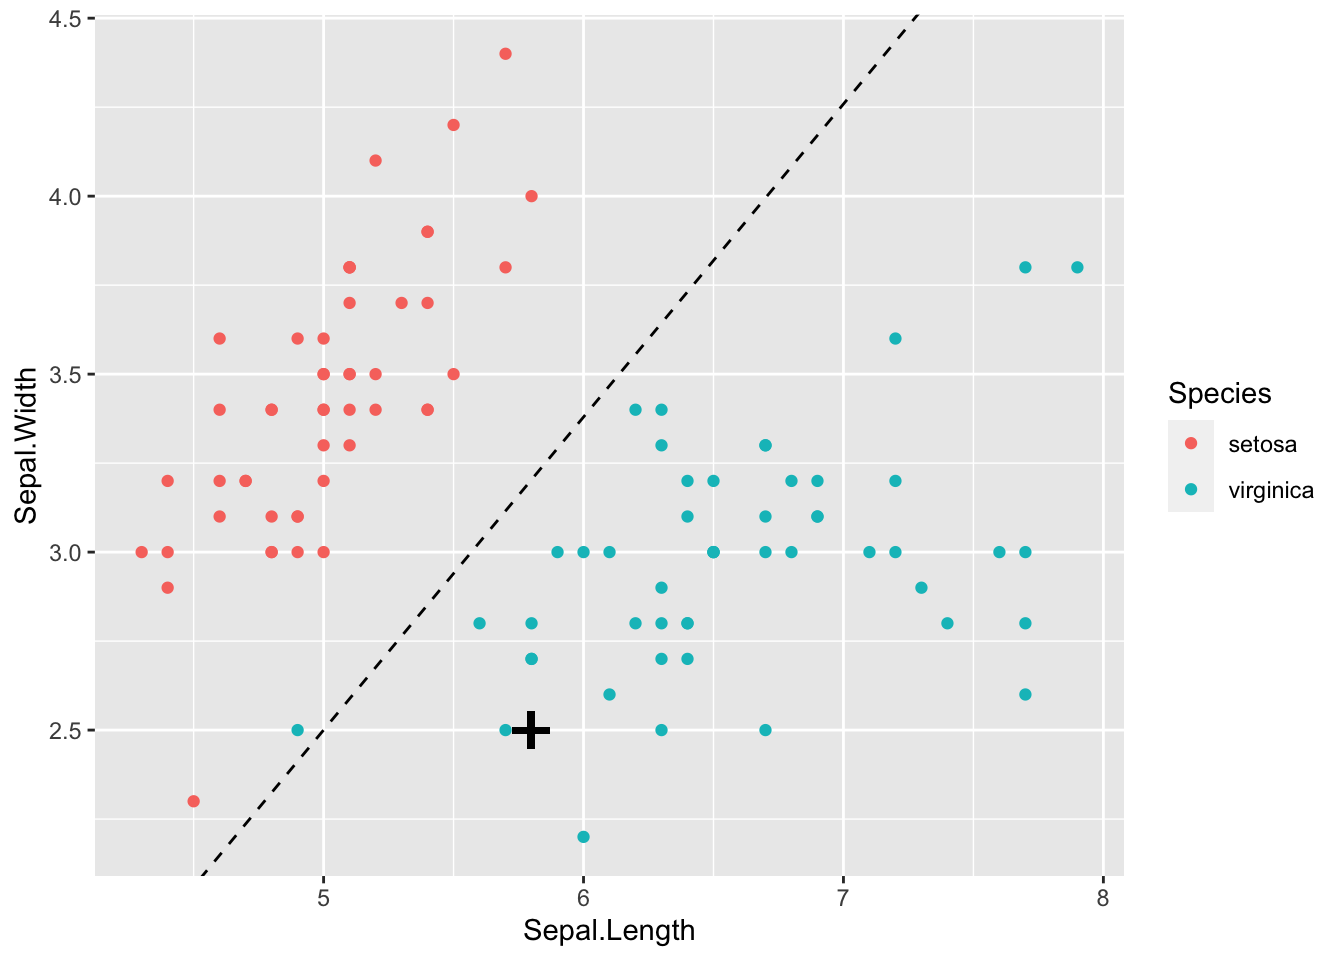
\includegraphics[width=1\linewidth]{03-matrix-decompositions_files/figure-latex/unnamed-chunk-12-1}

This is a \(512 \times 512\) colour image, meaning that there are three matrices \(\mathbf R, \mathbf B,\mathbf G\) of dimension \(512\times 512\)) giving the intensity of red, green, and blue for each pixel.
Naively storing this matrix requires 5.7Mb.

We can compute the SVD of the three colour intensity matrices, and the view the image that results from using reduced rank versions \(\mathbf B_k, \mathbf G_k, \mathbf R_k\) instead (as in Equation \eqref{eq:svdreduced}). The image below is formed using \(k=5, 30, 100\), and \(300\) basis vectors.

\begin{Shaded}
\begin{Highlighting}[]
\NormalTok{svd_image <-}\StringTok{ }\ControlFlowTok{function}\NormalTok{(im,k)\{}
\NormalTok{  s <-}\StringTok{ }\KeywordTok{svd}\NormalTok{(im)}
\NormalTok{  Sigma_k <-}\StringTok{ }\KeywordTok{diag}\NormalTok{(s}\OperatorTok{$}\NormalTok{d[}\DecValTok{1}\OperatorTok{:}\NormalTok{k])}
\NormalTok{  U_k <-}\StringTok{ }\NormalTok{s}\OperatorTok{$}\NormalTok{u[,}\DecValTok{1}\OperatorTok{:}\NormalTok{k]}
\NormalTok{  V_k <-}\StringTok{ }\NormalTok{s}\OperatorTok{$}\NormalTok{v[,}\DecValTok{1}\OperatorTok{:}\NormalTok{k]}
\NormalTok{  im_k <-}\StringTok{ }\NormalTok{U_k }\OperatorTok\StringTok{ }\NormalTok{Sigma_k }\OperatorTok\StringTok{ }\KeywordTok{t}\NormalTok{(V_k)}
   \CommentTok{## the reduced rank SVD produces some intensities <0 and >1. }
  \CommentTok{# Let's truncate these}
\NormalTok{  im_k[im_k}\OperatorTok{>}\DecValTok{1}\NormalTok{]=}\DecValTok{1}
\NormalTok{  im_k[im_k}\OperatorTok{<}\DecValTok{0}\NormalTok{]=}\DecValTok{0}
  \KeywordTok{return}\NormalTok{(im_k)}
\NormalTok{\}}

\KeywordTok{par}\NormalTok{(}\DataTypeTok{mfrow=}\KeywordTok{c}\NormalTok{(}\DecValTok{2}\NormalTok{,}\DecValTok{2}\NormalTok{), }\DataTypeTok{mar=}\KeywordTok{c}\NormalTok{(}\DecValTok{1}\NormalTok{,}\DecValTok{1}\NormalTok{,}\DecValTok{1}\NormalTok{,}\DecValTok{1}\NormalTok{))}

\NormalTok{pepprssvd<-}\StringTok{ }\NormalTok{peppers}
\ControlFlowTok{for}\NormalTok{(k }\ControlFlowTok{in} \KeywordTok{c}\NormalTok{(}\DecValTok{4}\NormalTok{,}\DecValTok{30}\NormalTok{,}\DecValTok{100}\NormalTok{,}\DecValTok{300}\NormalTok{))\{}
\NormalTok{  svds<-}\KeywordTok{list}\NormalTok{()}
  \ControlFlowTok{for}\NormalTok{(ii }\ControlFlowTok{in} \DecValTok{1}\OperatorTok{:}\DecValTok{3}\NormalTok{) \{}
\NormalTok{    pepprssvd[,,ii]<-}\KeywordTok{svd_image}\NormalTok{(peppers[,,ii],k)}
\NormalTok{  \}}
  \KeywordTok{plot}\NormalTok{(}\KeywordTok{as.raster}\NormalTok{(pepprssvd))}
\NormalTok{\}}
\end{Highlighting}
\end{Shaded}

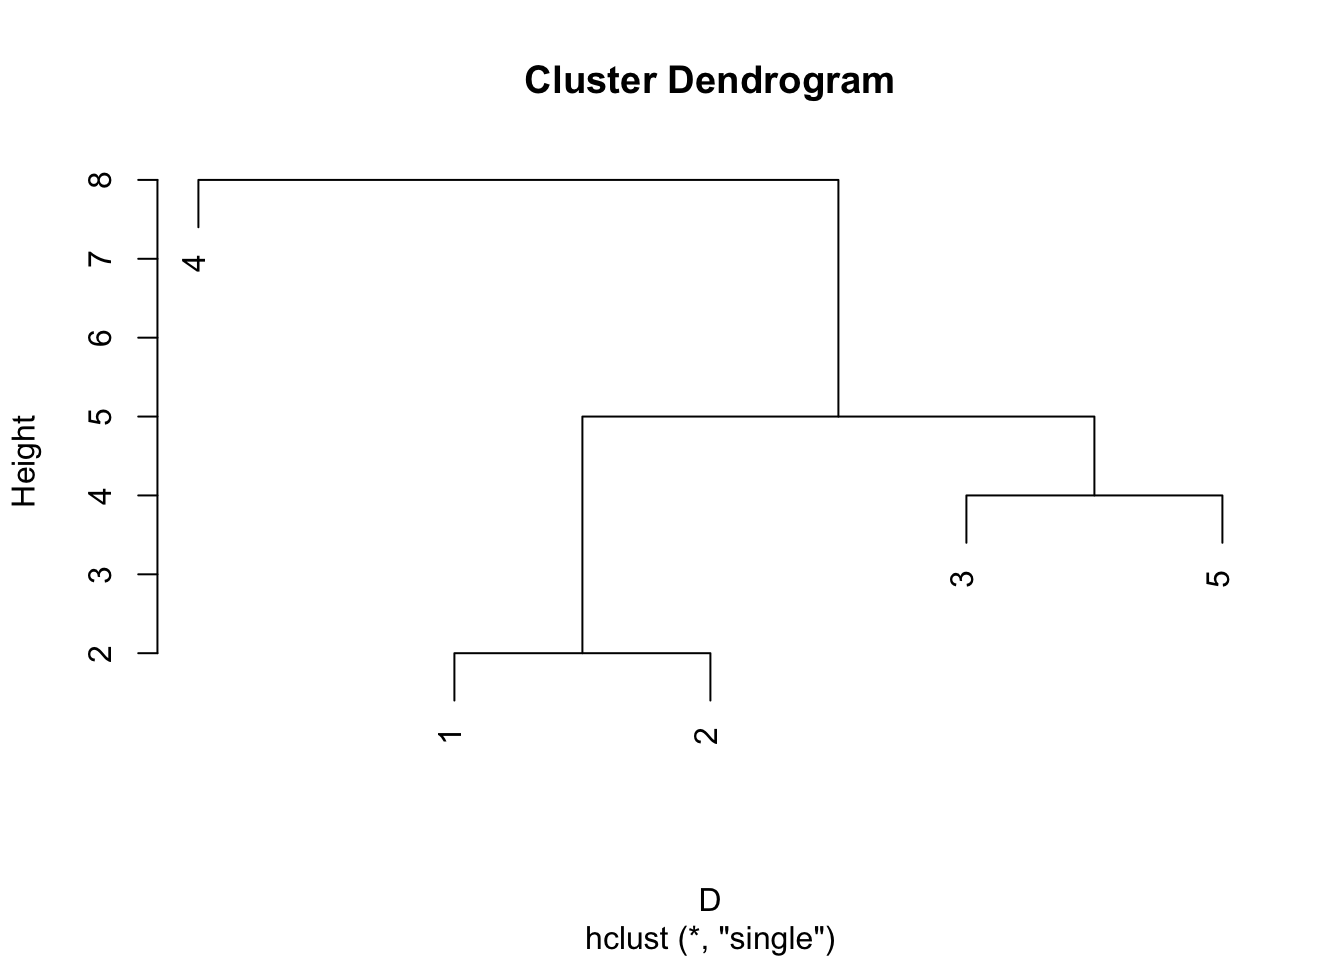
\includegraphics[width=1\linewidth]{03-matrix-decompositions_files/figure-latex/unnamed-chunk-13-1}

You can see that for \(k=30\) we have a reasonable approximation, but with some errors. With \(k=100\) it is hard to spot the difference with the original. The size of the four compressed images is 45Kb, 345Kb, 1.1Mb and 3.4Mb.

You can see further demonstrations of image compression with the SVD \href{http://timbaumann.info/svd-image-compression-demo/}{here}.

We will see much more of the SVD in later chapters.

\hypertarget{tasks-ch3}{%
\section{Computer tasks}\label{tasks-ch3}}

\begin{enumerate}
\def\labelenumi{\arabic{enumi}.}
\tightlist
\item
  Finding the eigenvalues and eigenvectors of a matrix is easy in R.
\end{enumerate}

\begin{Shaded}
\begin{Highlighting}[]
\NormalTok{A=}\KeywordTok{matrix}\NormalTok{(}\KeywordTok{c}\NormalTok{(}\DecValTok{3}\NormalTok{,}\DecValTok{1}\NormalTok{,}\DecValTok{1}\NormalTok{,}\DecValTok{6}\NormalTok{),}\DataTypeTok{nrow=}\DecValTok{2}\NormalTok{,}\DataTypeTok{byrow=}\OtherTok{TRUE}\NormalTok{)    }\CommentTok{# use a to define a matrix A}
\NormalTok{Eig=}\KeywordTok{eigen}\NormalTok{(A)                     }\CommentTok{# the eigenvalues and eigenvectors of A}
                                   \CommentTok{# are stored in the list Eig}
\NormalTok{lambda=Eig}\OperatorTok{$}\NormalTok{values                }\CommentTok{# extract the eigenvalues from Eig and}
                                   \CommentTok{# store in the vector e}
\NormalTok{lambda                           }\CommentTok{# you should see the eigenvalues in}
\end{Highlighting}
\end{Shaded}

\begin{verbatim}
## [1] 6.302776 2.697224
\end{verbatim}

\begin{Shaded}
\begin{Highlighting}[]
                                   \CommentTok{# descending order}
\NormalTok{Q=Eig}\OperatorTok{$}\NormalTok{vectors                    }\CommentTok{# extract the eigenvectors from Eig and}
                                   \CommentTok{# store then in the columns of Q}
\end{Highlighting}
\end{Shaded}

The spectral decomposition of \(\mathbf A\) is
\[\mathbf A= \mathbf Q\boldsymbol \Lambda\mathbf Q^\top\]
Let's check this in R (noting as always that there may be some numerical errors)

\begin{Shaded}
\begin{Highlighting}[]
\NormalTok{Q}\OperatorTok\KeywordTok{diag}\NormalTok{(lambda)}\OperatorTok\KeywordTok{t}\NormalTok{(Q)          }\CommentTok{# reconstruct A,}
\end{Highlighting}
\end{Shaded}

\begin{verbatim}
##      [,1] [,2]
## [1,]    3    1
## [2,]    1    6
\end{verbatim}

\begin{Shaded}
\begin{Highlighting}[]
                                   \CommentTok{# where t(Q) gives the transpose of Q}
\end{Highlighting}
\end{Shaded}

Since A is positive definite, we can calculate the symmetric, positive definite square root of A.

\begin{Shaded}
\begin{Highlighting}[]
\NormalTok{Asqrt=Q}\OperatorTok\KeywordTok{diag}\NormalTok{(lambda}\OperatorTok{**}\FloatTok{0.5}\NormalTok{)}\OperatorTok\KeywordTok{t}\NormalTok{(Q) }\CommentTok{# lambda**0.5 contains the square roots}
\NormalTok{Asqrt}\OperatorTok\NormalTok{Asqrt                      }\CommentTok{# it is seen that A is recovered}
\end{Highlighting}
\end{Shaded}

\begin{verbatim}
##      [,1] [,2]
## [1,]    3    1
## [2,]    1    6
\end{verbatim}

\begin{itemize}
\tightlist
\item
  Instead of using the full eigendecomposition for \(\mathbf A\), try truncating it and using just a single eigenvalue and eigenvector, i.e., compute
  \[\mathbf A' = \lambda_1 \mathbf q_1 \mathbf q_1^\top\]
\item
  Compute the difference between \(\mathbf A\) and \(\mathbf A'\) using the 2-norm and the Frobenius norm.
\end{itemize}

\begin{enumerate}
\def\labelenumi{\arabic{enumi}.}
\setcounter{enumi}{1}
\tightlist
\item
  The singular value decomposition can be computed in R using the command \texttt{svd}. Let \(\mathbf X\) be the four numerical variables in the \texttt{iris} dataset with the column mean removed
\end{enumerate}

\begin{Shaded}
\begin{Highlighting}[]
\NormalTok{n=}\DecValTok{150}
\NormalTok{H=}\KeywordTok{diag}\NormalTok{(}\KeywordTok{rep}\NormalTok{(}\DecValTok{1}\NormalTok{,n))}\OperatorTok{-}\KeywordTok{rep}\NormalTok{(}\DecValTok{1}\NormalTok{,n)}\OperatorTok\KeywordTok{t}\NormalTok{(}\KeywordTok{rep}\NormalTok{(}\DecValTok{1}\NormalTok{,n))}\OperatorTok{/}\NormalTok{n   }\CommentTok{# calculate the centering matrix H}
\NormalTok{X=H}\OperatorTok\StringTok{ }\KeywordTok{as.matrix}\NormalTok{(iris[,}\DecValTok{1}\OperatorTok{:}\DecValTok{4}\NormalTok{])}
\CommentTok{# This can also be done using the command}
\CommentTok{# sweep(iris[,1:4], 2, colMeans(iris[,1:4]))  # do you understand why?}
\end{Highlighting}
\end{Shaded}

\begin{itemize}
\item
  Compute the SVD of \(\mathbf X\) in R and report its singular values.
\item
  Does R report the full or compact SVD?
\item
  Check that \(\mathbf X\mathbf v= \sigma \mathbf u\).
\item
  Compute the best rank-1, rank-2, and rank-3 approximations to \(\mathbf X\), and report the 2-norm and Frobenious norm for these approximations
\item
  Compute the eigenvalues of \(\mathbf X^\top \mathbf X\). How do these relate to the singular values? How does \(\mathbf X^\top \mathbf X\) relate to the sample covariance matrix of the iris data? How do the singular values relate to the eigenvalues of the covariance matrix?
\item
  Let \(\mathbf S\) be the sample covariance matrix of the iris dataset. What vector \(\mathbf x\) with \(||\mathbf x||=1\) maximizes \(\mathbf x^\top \mathbf S\mathbf x\)?
\end{itemize}

\begin{enumerate}
\def\labelenumi{\arabic{enumi}.}
\setcounter{enumi}{2}
\tightlist
\item
  Choose an few images from the \href{http://sipi.usc.edu/database/}{USC-SIPI Image Database} and repeat the image compression example from the notes. Which type of images compress well do you think?
\end{enumerate}

\hypertarget{exercises-ch3}{%
\section{Exercises}\label{exercises-ch3}}

\begin{enumerate}
\def\labelenumi{\arabic{enumi}.}
\tightlist
\item
  Let \(\boldsymbol{\Sigma}\) be an arbitrary covariance matrix.

  \begin{itemize}
  \tightlist
  \item
    Show \(\boldsymbol{\Sigma}\) is symmetric and
    non-negative definite.
  \item
    Give examples of both singular and non-singular covariance matrices.\\
  \item
    What condition must the eigenvalues of a non-singular covariance matrix satisfy?
  \end{itemize}
\end{enumerate}

\begin{enumerate}
\def\labelenumi{\arabic{enumi}.}
\setcounter{enumi}{1}
\tightlist
\item
  Compute, by hand (but check your answer in R), the singular value decomposition (full and compact) of the following matrices.

  \begin{itemize}
  \tightlist
  \item
    \(\left(\begin{array}{cc}2&0\\0&-1\end{array} \right)\)
  \item
    \(\left(\begin{array}{cc}1&0\\0&0\\0&0\end{array} \right)\)
  \end{itemize}
\item
  Let \[\mathbf X=\left(\begin{array}{cc}1&1\\0&1\\1&0\end{array}
  \right)\]\\
  The eigen-decomposition of \(\mathbf X^\top \mathbf X\) is
  \[\mathbf X^\top \mathbf X=\frac{1}{\sqrt{2}}\left(\begin{array}{cc}1&-1\\1&1\end{array}
  \right) \left(\begin{array}{cc}3&0\\0&1\end{array}
  \right)\frac{1}{\sqrt{2}}\left(\begin{array}{cc}1&-1\\1&1\end{array}
  \right)^\top \]
  Use this fact to compute answer the following questions:

  \begin{itemize}
  \tightlist
  \item
    What are the singular values of \(\mathbf X\)?
  \item
    What are the right singular vectors of \(\mathbf X\)?
  \item
    What are the left singular vectors of \(\mathbf X\)?
  \item
    Give the compact SVD of \(\mathbf X\). Check your answer, noting that the singular vectors are only specified up to multiplication by \(-1\)
  \item
    Can you compute the full SVD of \(\mathbf X\)?
  \item
    What is the eigen-decomposition of \(\mathbf X\mathbf X^\top\)?
  \item
    Find a generalised inverse of matrix \(\mathbf X\).
  \end{itemize}
\end{enumerate}

\begin{enumerate}
\def\labelenumi{\arabic{enumi}.}
\setcounter{enumi}{3}
\item
  The SVD can be used to solve linear systems of the form
  \[\mathbf A\mathbf x= \mathbf y\]
  where \(\mathbf A\) is a \(n\times p\) matrix, with compact SVD
  \(\mathbf A= \mathbf U\boldsymbol{\Sigma}\mathbf V^\top\).

  \begin{itemize}
  \item
    If \(\mathbf A\) is a square invertible matrix, show that \[\tilde{\mathbf x} = \mathbf V\boldsymbol{\Sigma}^{-1} \mathbf U^\top \mathbf y\] is the unique solution to \(\mathbf A\mathbf x= \mathbf y\), i.e., show that \(\mathbf A^{-1} = \mathbf V\boldsymbol{\Sigma}^{-1} \mathbf U^\top\).
  \item
    If \(\mathbf A\) is not a square matrix, then \(\mathbf A^+ = \mathbf V\boldsymbol{\Sigma}^{-1} \mathbf U^\top\) is a generalized inverse (not a true inverse) matrix, and
    \(\tilde{\mathbf x}=\mathbf A^+\mathbf y\) is still a useful quantity to consider as we shall now see. Let \(\mathbf A=\left(\begin{array}{cc}1&1\\0&1\\1&0\end{array} \right)\) and \(\mathbf y= \left(\begin{array}{c}2\\1\\1\end{array} \right)\). Then \(\mathbf A\mathbf x=\mathbf y\) is an over-determined system in that there are 3 equations in 2 unknowns. Compute \(\tilde{\mathbf x}=\mathbf A^+\mathbf y\). Is this a solution to the equation?
  \end{itemize}

  \textbf{Note} that you computed the svd for \(\mathbf A\) in Q2.

  \begin{itemize}
  \tightlist
  \item
    Now suppose \(\mathbf y= \left(\begin{array}{c}1\\-1\\1\end{array} \right)\). There is no solution to \(\mathbf A\mathbf x=\mathbf y\) in this case as \(\mathbf y\) is not in the column space of \(\mathbf A\). Prove that \({\tilde{\mathbf x}} = \mathbf A^+\mathbf y\) solves the least squares problem
    \[\tilde{\mathbf x} = \arg\min_{\mathbf x}||\mathbf y- \mathbf A\mathbf x||_2.\]
  \end{itemize}

  \textbf{Hint}: You can either do this directly for this problem, or you can show that the least squares solution \((\mathbf A^\top \mathbf A)^{-1}\mathbf A^\top \mathbf y=\tilde{\mathbf x}\).
\item
  Consider the system
  \[\mathbf B\mathbf x= \mathbf y\mbox{ with }\mathbf B=\left(\begin{array}{ccc}1&0&1\\1&1&0\end{array}
  \right),\mathbf y= \left(\begin{array}{c}1\\1\end{array}
  \right).\]
  This is an underdetermined system, as there are 2 equations in 3 unknowns, and so there are an infinite number of solutions for \(\mathbf x\) in this case.

  \begin{itemize}
  \tightlist
  \item
    Find the full SVD for \(\mathbf B=\mathbf U\boldsymbol{\Sigma}\mathbf V^\top\) (noting that \(\mathbf B=\mathbf A^\top\) for \(\mathbf A\) from the previous question).
  \item
    Compute
    \(\tilde{\mathbf x}=\mathbf B^+\mathbf y\), check it is a solution to the equation, and explain why \[\tilde{\mathbf x}= \sum_{i=1}^r \mathbf v_i \frac{\mathbf u_i^\top \mathbf y}{\sigma_i}\] in general, where \(r\leq max(n,p)\) is the rank of \(\mathbf B\), and write out \(\tilde{\mathbf x}\) explicitly in this form for the given \(\mathbf B\).
  \item
    Consider \(\mathbf x\) of the form
    \[\mathbf x= \tilde{\mathbf x} + \sum_{i=r+1}^n \alpha_i \mathbf v_i\]
    and explain why any \(\mathbf x\) of this form is also a solution to \(\mathbf B\mathbf x=\mathbf y\). Thus write out all possible solutions of the equation.
  \item
    Prove that \(\tilde{\mathbf x}\) is the solution with minimum norm, i.e., \(||\tilde{\mathbf x}||_2 \leq ||\mathbf x||_2\). \textbf{Hint} \(\mathbf v_1, \ldots, \mathbf v_p\) form a complete orthonormal basis for \(\mathbb{R}^p\).
  \end{itemize}
\item
  Prove proposition \ref{prp:eigproj}.
\end{enumerate}

\hypertarget{part-ii-dimension-reduction-methods}{%
\chapter*{PART II: Dimension reduction methods}\label{part-ii-dimension-reduction-methods}}
\addcontentsline{toc}{chapter}{PART II: Dimension reduction methods}

\href{https://mediaspace.nottingham.ac.uk/media/Part+IIA+Dimension+reduction+introduction/1_0s2cgr1r}{Introductory Video}

In many applications, a large number of variables are recorded for each experimental unit under study. For example, if we think of individual people as the \emph{experimental units}, then in a health check-up we might collect data on age, blood pressure, cholesterol level, blood test results, lung function, weight, height, BMI, etc. If you use websites such as Amazon, Facebook, and Google, they store thousands (possibly millions) of pieces of information about you (\href{https://www.theguardian.com/commentisfree/2018/mar/28/all-the-data-facebook-google-has-on-you-privacy}{this article} shows you how to download the information Google stores about you, including all the locations you've visited, every search, youtube video, or app you've used and more). They process this data to create an individual profile for each user, which they can then use to create targetted adverts.

When analysing data of moderate or high dimension, it is often desirable to seeks ways to restructure the data and reduce its dimension whilst \textbf{retaining the most important information} within the data or \textbf{preserving some feature of interest} in the data. There a variety of reasons we might want to do this.

\begin{itemize}
\tightlist
\item
  In reduced dimensions, it is often much easier to understand and appreciate the most important features of a dataset.
\item
  If there is a lot of reduncancy in the data, we might want to reduce the dimension to lower the memory requirements in storing it (e.g.~with sound and image compression).
\item
  In high dimensions, it can be difficult to analyse data (e.g.~with statistical methods), and so reducing the dimension can be a way to make a dataset amenable to analysis.
\end{itemize}

In this part of the module we investigate three different methods for dimension reduction: Principal Component Analysis (PCA) in Chapter \ref{pca}; Canonical Correlation Analysis (CCA) in Chapter \ref{cca}; and Multidimensional Scaling (MDS) in Chapter \ref{mds}. Matrix algebra (Chapters \ref{linalg-prelim} and \ref{linalg-decomp}) plays a key role in all three of these techniques.

\hypertarget{a-warning}{%
\subsection*{A warning}\label{a-warning}}
\addcontentsline{toc}{subsection}{A warning}

Beware that high-dimensional data can behave qualitatively differently to low-dimensional data. As an example, lets consider 1000 points uniformly distributed in \([0,1]^d\), and think about how close together or spread out the points are. A simple way to do this is to consider the ratio of the maximum and minimum distance between any two points in our sample.

\begin{Shaded}
\begin{Highlighting}[]
\NormalTok{N<-}\DecValTok{1000}
\NormalTok{averatio <-}\KeywordTok{c}\NormalTok{()}
\NormalTok{ii<-}\DecValTok{1}
\ControlFlowTok{for}\NormalTok{(d }\ControlFlowTok{in} \KeywordTok{c}\NormalTok{(}\DecValTok{2}\NormalTok{,}\DecValTok{5}\NormalTok{,}\DecValTok{10}\NormalTok{,}\DecValTok{20}\NormalTok{,}\DecValTok{30}\NormalTok{,}\DecValTok{40}\NormalTok{,}\DecValTok{50}\NormalTok{,}\DecValTok{60}\NormalTok{,}\DecValTok{80}\NormalTok{,}\DecValTok{100}\NormalTok{, }\DecValTok{200}\NormalTok{, }\DecValTok{350}\NormalTok{, }\DecValTok{500}\NormalTok{, }\DecValTok{750}\NormalTok{, }\DecValTok{1000}\NormalTok{))\{}
\NormalTok{  averatio[ii] <-}\StringTok{ }\KeywordTok{mean}\NormalTok{(}\KeywordTok{replicate}\NormalTok{(}\DecValTok{10}\NormalTok{, \{}
\NormalTok{  X<-}\KeywordTok{matrix}\NormalTok{(}\KeywordTok{runif}\NormalTok{(N}\OperatorTok{*}\NormalTok{d), }\DataTypeTok{nc=}\NormalTok{d)}
\NormalTok{  d <-}\StringTok{ }\KeywordTok{as.matrix}\NormalTok{(}\KeywordTok{dist}\NormalTok{(X)) }
  \CommentTok{# this gives a N x N matrix of the Euclidean distances between the data points.}
\NormalTok{  maxdist <-}\StringTok{ }\KeywordTok{max}\NormalTok{(d) }
\NormalTok{  mindist <-}\StringTok{ }\KeywordTok{min}\NormalTok{(d}\OperatorTok{+}\KeywordTok{diag}\NormalTok{(}\DecValTok{10}\OperatorTok{^}\DecValTok{5}\NormalTok{, }\DataTypeTok{nrow=}\NormalTok{N)) }
  \CommentTok{# The diagonal elements of the distance matrix are zero,}
  \CommentTok{# so I've added a big number to the diagonal }
  \CommentTok{# so that we get the minimum distance between different points}
\NormalTok{  maxdist}\OperatorTok{/}\NormalTok{mindist\}))}
\NormalTok{  ii <-}\StringTok{ }\NormalTok{ii}\OperatorTok{+}\DecValTok{1}
\NormalTok{\}}
\KeywordTok{plot}\NormalTok{(}\KeywordTok{c}\NormalTok{(}\DecValTok{2}\NormalTok{,}\DecValTok{5}\NormalTok{,}\DecValTok{10}\NormalTok{,}\DecValTok{20}\NormalTok{,}\DecValTok{30}\NormalTok{,}\DecValTok{40}\NormalTok{,}\DecValTok{50}\NormalTok{,}\DecValTok{60}\NormalTok{,}\DecValTok{80}\NormalTok{,}\DecValTok{100}\NormalTok{, }\DecValTok{200}\NormalTok{, }\DecValTok{350}\NormalTok{, }\DecValTok{500}\NormalTok{, }\DecValTok{750}\NormalTok{, }\DecValTok{1000}\NormalTok{), }
\NormalTok{     averatio, }\DataTypeTok{ylab=}\StringTok{'Max. dist. / min. dist.'}\NormalTok{, }\DataTypeTok{xlab=}\StringTok{'Dimension d'}\NormalTok{, }\DataTypeTok{log=}\StringTok{'xy'}\NormalTok{)}
\end{Highlighting}
\end{Shaded}

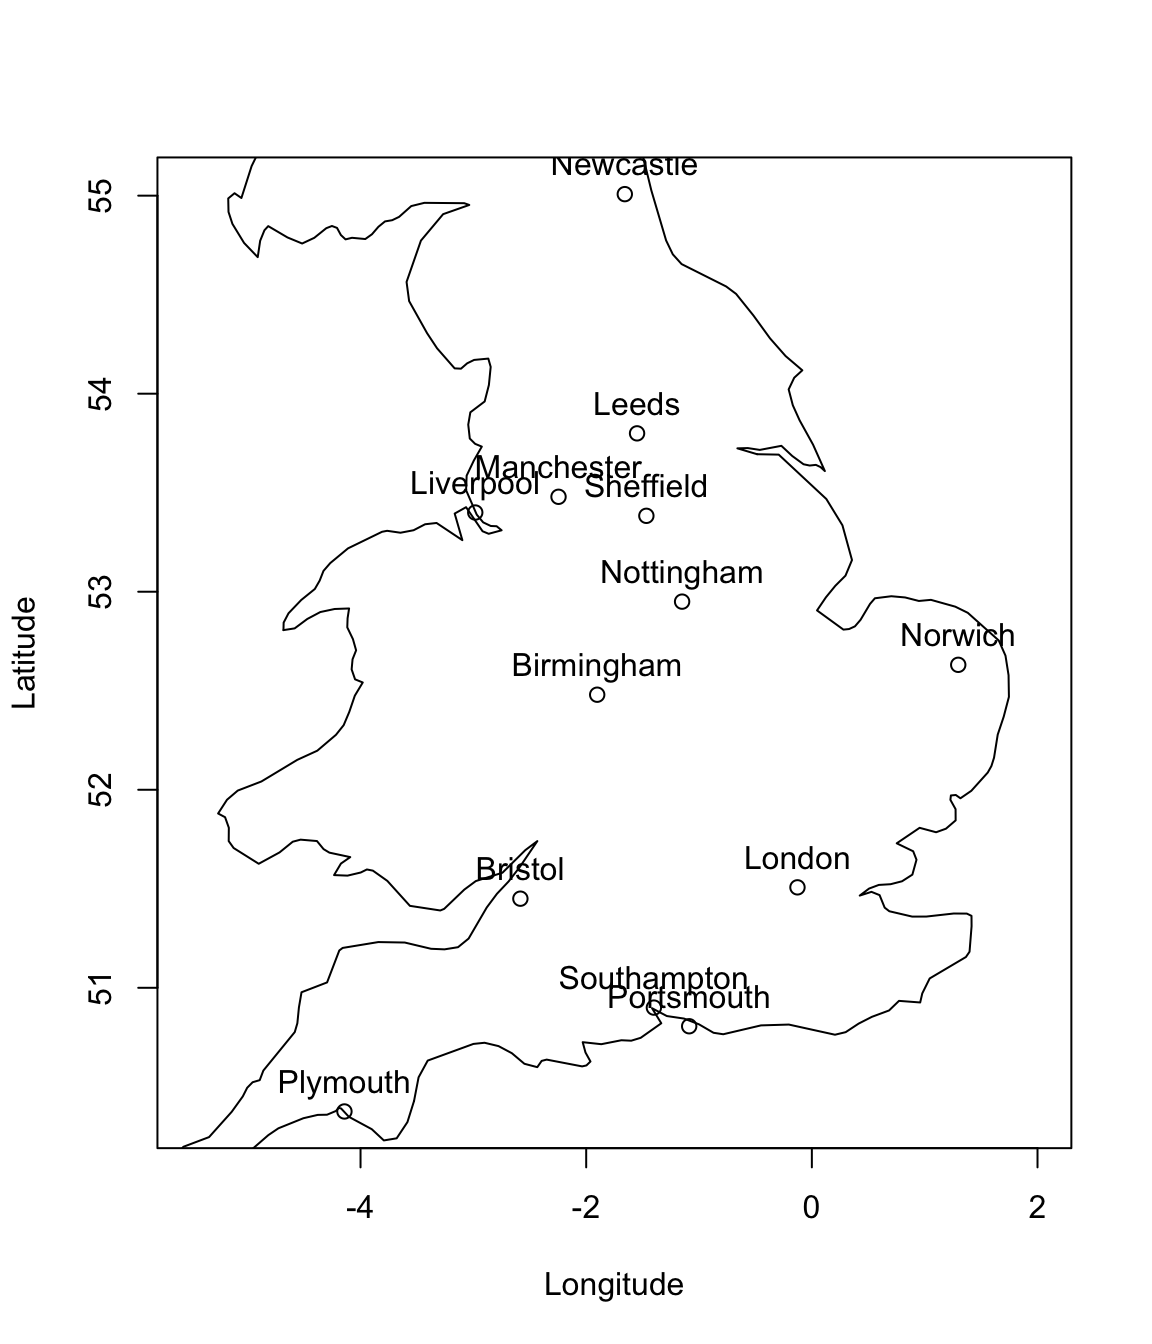
\includegraphics{04-pca_files/figure-latex/unnamed-chunk-1-1.pdf}

So we can see that as the dimension increases, the ratio of the maximum and minimum distance between any two random points in our sample tends to 1. In other words, all points are the same distance apart!

\hypertarget{pca}{%
\chapter{Principal Component Analysis (PCA)}\label{pca}}

The videos for this chapter are available at the following links:

\begin{itemize}
\tightlist
\item
  \href{https://mediaspace.nottingham.ac.uk/media/PCA_Informal/1_zs9dumou}{4.1 An informal introduction to PCA}
\item
  \href{https://mediaspace.nottingham.ac.uk/media/PCA+Informal+Examples/1_3c9ghrtf}{4.1.5 Informal Examples}
\item
  \href{https://mediaspace.nottingham.ac.uk/media/PCA+Formal+Description/1_tq8tpcn0}{4.2 A more formal description of PCA}
\item
  \href{https://mediaspace.nottingham.ac.uk/media/PCA+Properties/1_s2ldu6a7}{4.2.1 Properties of PC scores}
\item
  \href{https://mediaspace.nottingham.ac.uk/media/PCA+Football+Example/1_h70vgqq2}{4.2.2 Example: PCA of the football data}
\item
  \href{https://mediaspace.nottingham.ac.uk/media/Population+PCA+and+transformations/1_y1s2arei}{4.2.4 Population PCA and transformations}
\item
  \href{https://mediaspace.nottingham.ac.uk/media/PCAA+Minimizing+Reconstruction+Error/1_93tzf0ju}{4.3 An alternative view of PCA: minimizing reconstruction error`}
\item
  \href{https://mediaspace.nottingham.ac.uk/media/PCAA+MNIST+example/1_ljte3zc1}{4.3.1 Example: PCA of the MNIST data}
\end{itemize}

With multivariate data, it is common to want to reduce the dimension of the data \emph{in a sensible way}. For example

\begin{itemize}
\item
  exam marks across different modules are
  averaged to produce a single overall mark for each
  student
\item
  a football league table converts the
  numbers of wins, draws and losses to a single measure of
  points.
\end{itemize}

Mathematically, these summaries
are both linear combinations of the
original variables of the form
\[y = \mathbf u^\top \mathbf x.\]\\
for some choice of \(\mathbf u\).

For the exam marks example, suppose each student sits \(p=4\) modules
with marks, \(x_1,x_2,x_3,x_4\). Then, writing \(\mathbf x=(x_1, x_2 , x_3, x_4)^\top\) and choosing \(\mathbf u= \left(\frac{1}{4}, \frac{1}{4}, \frac{1}{4}, \frac{1}{4} \right)^\top\)
gives an overall average,
\[ y =\mathbf u^\top \mathbf x= \begin{pmatrix} \frac{1}{4} & \frac{1}{4} & \frac{1}{4} & \frac{1}{4} \end{pmatrix} \begin{pmatrix} x_1 \\ x_2 \\ x_3 \\ x_4 \end{pmatrix} = \frac{x_1}{4} + \frac{x_2}{4} + \frac{x_3}{4} + \frac{x_4}{4}.\]

For the football league table, if \(w\) is the number of wins, \(d\) is the number of draws and \(l\) is the number of losses then, writing
\({\mathbf r}=(w,d,l)^\top\), we choose \(\mathbf u= \left(3,1,0 \right)^\top\) to get the points score
\[ y = \mathbf u^\top {\mathbf r}=\begin{pmatrix} 3 & 1 & 0 \end{pmatrix} \begin{pmatrix} w \\ d \\ l \end{pmatrix} = 3w + 1d + 0l=3w+d.\]

\hypertarget{geometric-interpretation}{%
\subsubsection*{Geometric interpretation}\label{geometric-interpretation}}
\addcontentsline{toc}{subsubsection}{Geometric interpretation}

In the two examples above, we used the vector \(\mathbf u\) to convert our original variables, \(\mathbf x\),
to a new variable, \(y\), by projecting \(\mathbf x\) onto \(\mathbf u\).
We can think of this as a projection onto the subspace defined by \(\mathbf u\)

\[U = \operatorname{span}\{\mathbf u\} = \{\lambda \mathbf u: \lambda \in \mathbb{R}\}\subset \mathbb{R}^p,\]

For the exam data, each data point \(\mathbf x= \begin{pmatrix} x_1 \\ x_2 \\ x_3 \\ x_4 \end{pmatrix}\)
is a vector in \(\mathbb{R}^4\), and we've expressed \(\mathbf x\) in terms of its coordinates with respsect to the standard basis, \(\mathbf e_1^\top = (1\; 0\; 0 \; 0)\) etc:
\[\mathbf x=x_1 \mathbf e_1 + x_2 \mathbf e_2 +x_3 \mathbf e_3 +x_4 \mathbf e_4.\]
The vector subspace \(U\) is a line in \(\mathbb{R}^4\) along the direction \(\mathbf u= \begin{pmatrix} \frac{1}{4} & \frac{1}{4} & \frac{1}{4} & \frac{1}{4} \end{pmatrix}^\top\).

How do we project onto subspace \(U\)?

\begin{itemize}
\tightlist
\item
  If \(||\mathbf u||_2=1\) then the orthogonal projection of \(\mathbf x\) onto \(U\) is\\
  \[\mathbf u\mathbf u^\top\mathbf x.\]
  Or in other words, the projection of \(\mathbf x\) onto subspace \(U\) has coordinate \(\mathbf u^\top \mathbf x\) with respect to basis \(\{\mathbf u\}\).
\end{itemize}

If you prefer to think in terms of projection matrices (see Chapter \ref{orthogproj}), then the matrix for projecting onto \(U\) is
\[\mathbf P_U = \mathbf u(\mathbf u^\top \mathbf u)^{-1}\mathbf u^\top\]
which simplifies to
\[\mathbf P_U = \mathbf u\mathbf u^\top\]
when \(||\mathbf u||=\sqrt{\mathbf u^\top\mathbf u}=1\) so that we again see the projection of \(\mathbf x\) onto \(U\) is \(y=\mathbf P_u \mathbf x= \mathbf u\mathbf u^\top\mathbf x\).

\textbf{How should we choose \(\mathbf u\)?}

The answer to that question depends upon the goal of the analysis. For the exam and football league examples, the choice of \(\mathbf u\) is an arbitrary decision taken in order to reduce a multidimensional dataset to a single variable (average mark, or points).

A single \(\mathbf u\) gives a \textbf{snapshot} or summary of the data. If \(\mathbf u\) is chosen well that snapshot may tell us much of what we want to know about the data, e.g.,

\begin{itemize}
\tightlist
\item
  Liverpool won the league,
\item
  student \(X\)'s exam performance was first class etc.
\end{itemize}

In many cases we will want to use multiple snapshots: instead of using a single \(\mathbf u\), we will use a collection \(\mathbf u_1, \mathbf u_2, \ldots, \mathbf u_r\) and consider the derived variables

\[\mathbf y= \begin{pmatrix} y_1\\y_2 \\ \vdots \\ y_r\end{pmatrix} = \begin{pmatrix}
\mathbf u_1^\top \mathbf x\\  \mathbf u_2^\top \mathbf x\\\vdots\\  \mathbf u_r^\top \mathbf x\end{pmatrix}\]

In matrix notation, if we set
\[\mathbf U= \begin{pmatrix} 
|&&|\\
\mathbf u_1 & \ldots & \mathbf u_r\\
|&&|\end{pmatrix}\]
then the new derived variable is
\[\mathbf y= \mathbf U^\top \mathbf x.\]

If \(\dim(\mathbf y)=r<p=\dim(\mathbf x)\) then we have reduced the dimension of the data. If \(\mathbf y\) tells us all we need to know about the data, then we can work (plot, analyse, model) with \(\mathbf y\) instead of \(\mathbf x\). If \(r\ll p\) this can make working with the data significantly easier, as we can more easily visulise and understand low dimensional problems.

We will study a variety of methods for choosing \(\mathbf U\). The methods can all be expressed as constrained optimization problems:

\begin{align}
\mbox{minimize} f_{\mathbf X}(\mathbf U) \label{eq:dimredopt} \\
\mbox{ subject to } \mathbf U\in \mathcal{U} 
\end{align}

The objective \(f_{\mathbf X}(\mathbf U)\) varies between methods: principal component analysis (PCA) maximizes variance or minimizes reconstruction error; canonical correlation analysis (CCA) maximizes correlation; multidimensional scaling (MDS) maximizes spread etc.

The contstraint on the search space \(\mathcal{U}\), is usually that \(\mathbf U\) must be (partially) orthogonal, but in other methods other constraints are used

\hypertarget{pca-an-informal-introduction}{%
\section{PCA: an informal introduction}\label{pca-an-informal-introduction}}

There are two different ways of motivating
principal component analysis (PCA), which may in part explain why PCA is so widely used.

The first motivation, and the topic of this section, is to introduce PCA as method for maximizing the variance of the transformed variables \(\mathbf y\). We start by choosing \(\mathbf u_1\) so that \(y_1=\mathbf u_1^\top \mathbf x\) has maximum variance. We then choose \(\mathbf u_2\) so that \(y_2=\mathbf u_2^\top \mathbf x\) has maximum variance subject to being uncorrelated with \(y_1\), and so on.

The idea is to produce a set of variables \(y_1, y_2, \ldots, y_r\) that are uncorrelated, but which are most informative about the data. The thinking is that if a variable has large variance it must be informative/important.

The name \textbf{principal component analysis} comes from thinking of this as splitting the data \(\mathbf X\) into its most important parts. It therefore won't surprise you to find that this involves the matrix decompositions we studied in Chapter \ref{linalg-decomp}.

\href{https://twitter.com/allison_horst/status/1288904459490213888?lang=en}{Allison Horst (@allison\_horst)} gave a great illustration of how to think about PCA on Twitter. Imagine you are a whale shark with a wide mouth

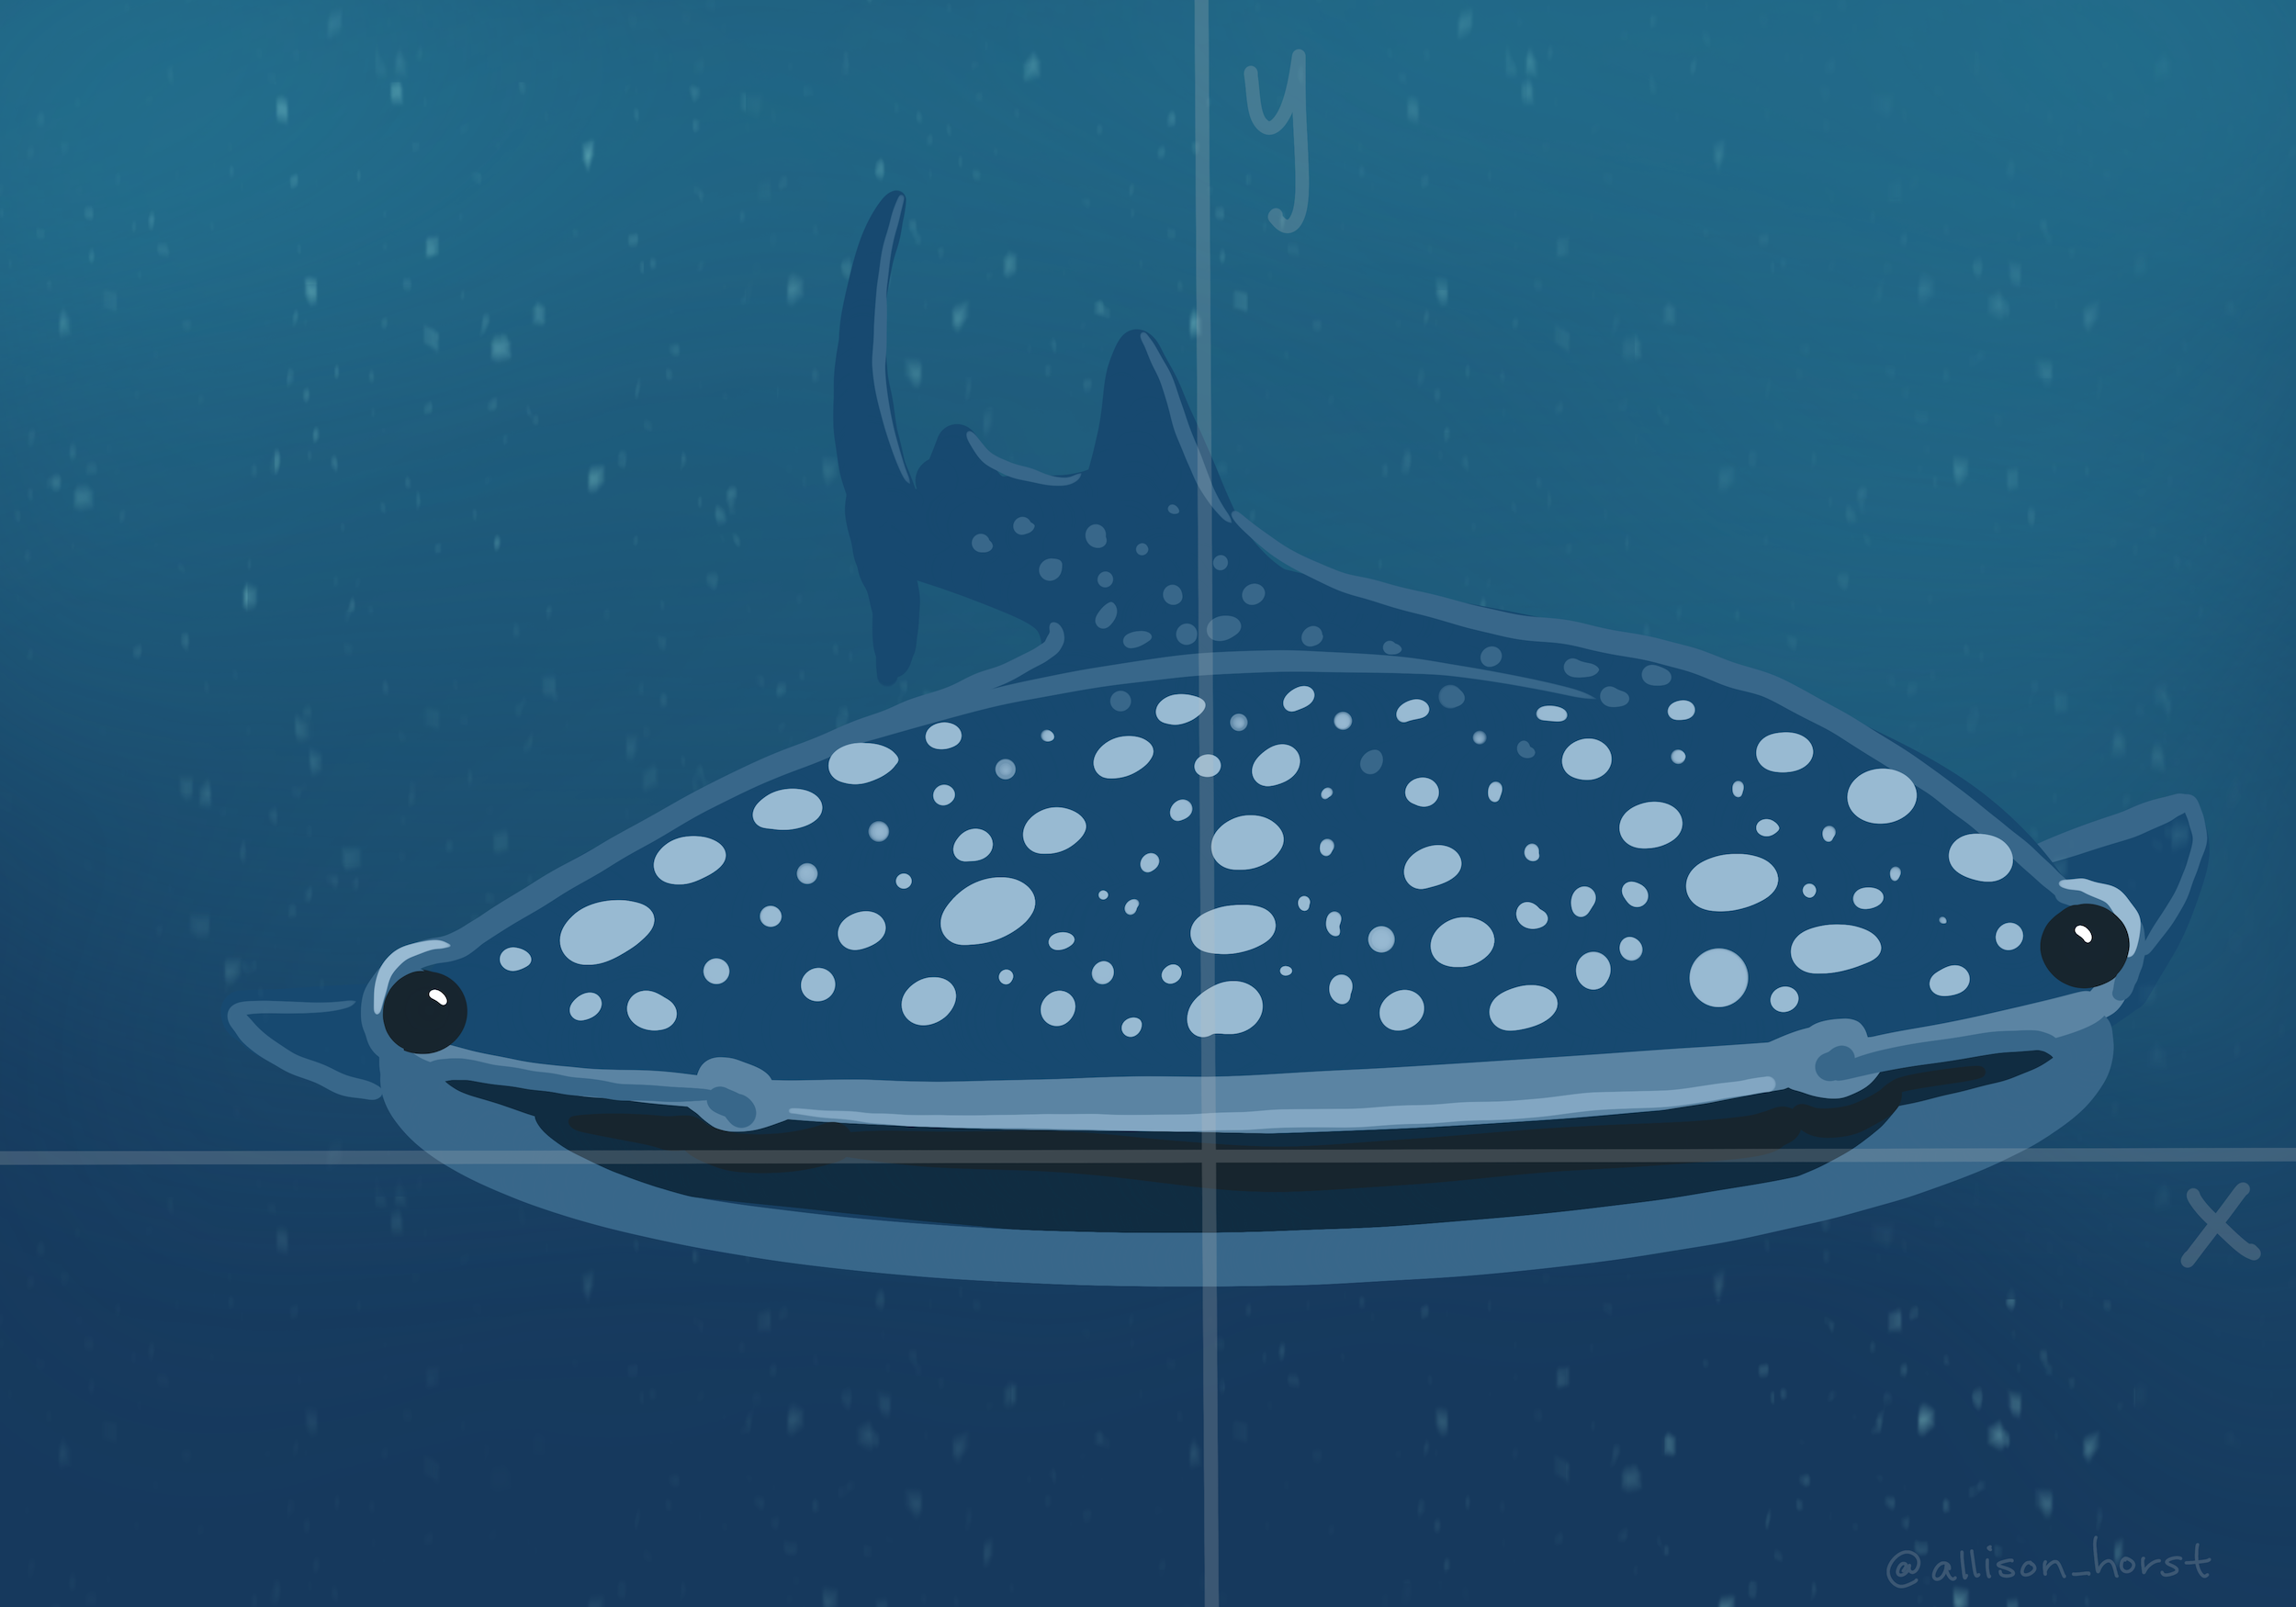
\includegraphics{figs/WideMouthShark1.png}

and that you're swimming towards a delicious swarm of krill.

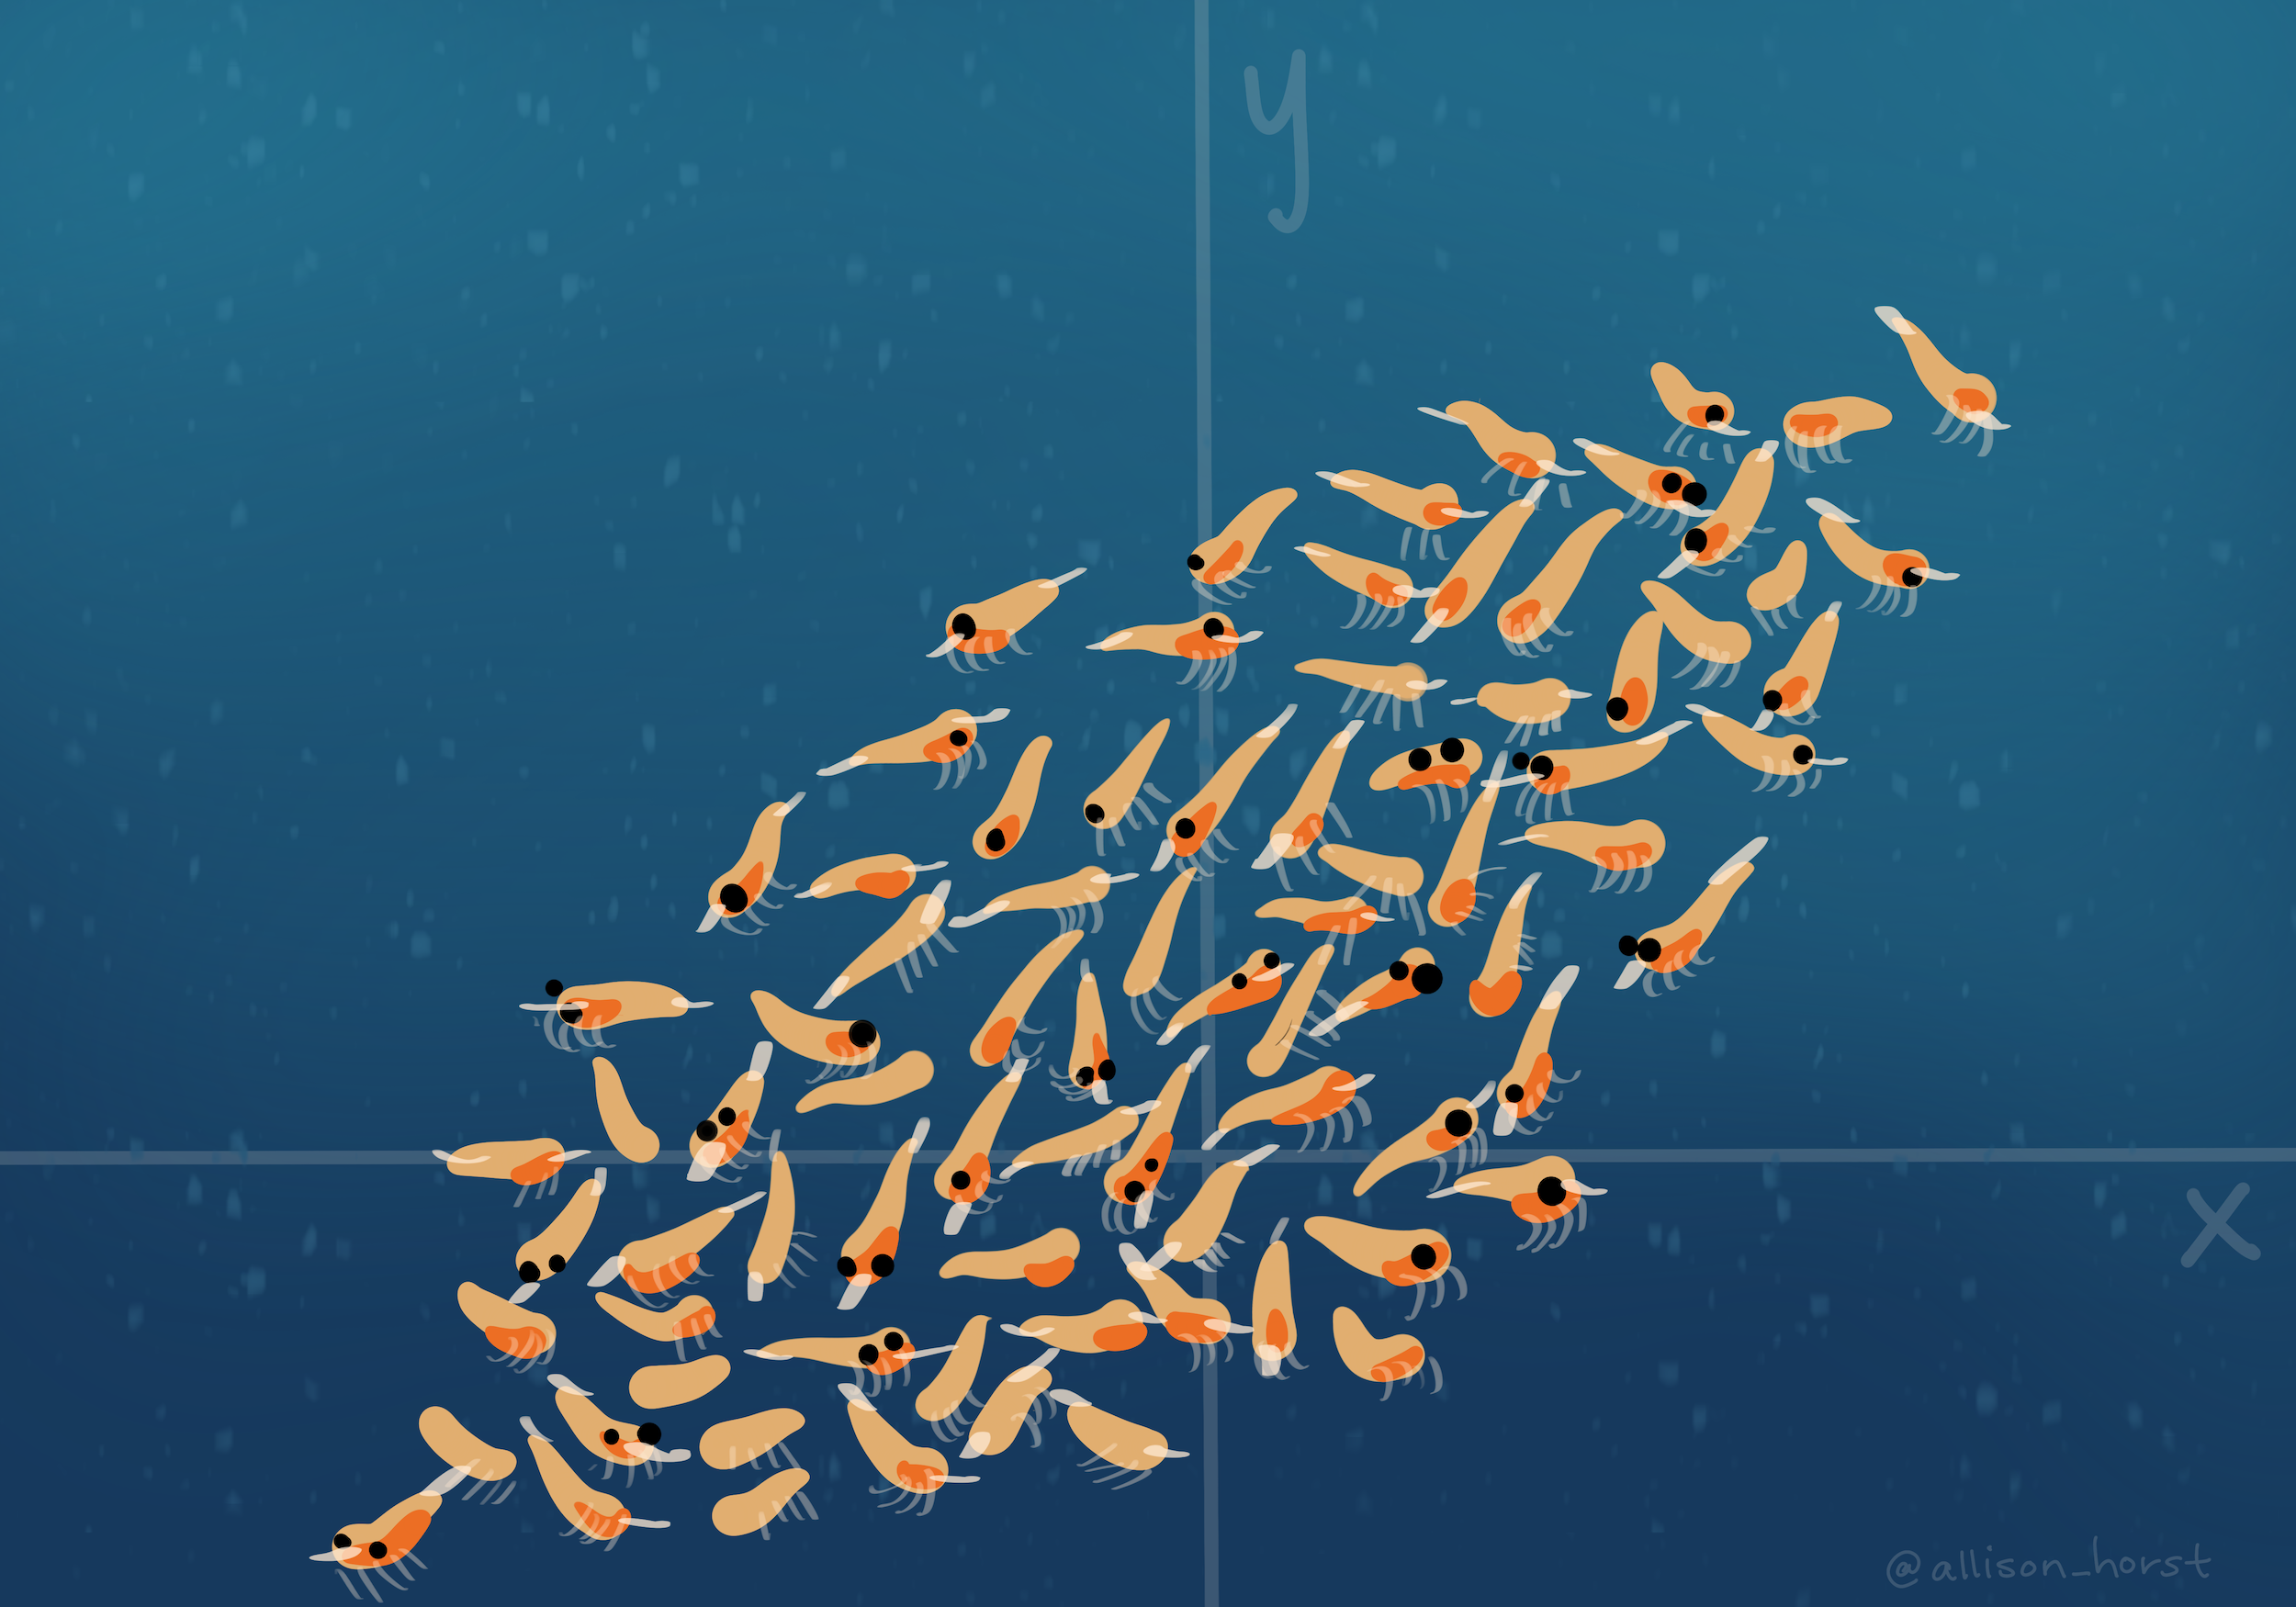
\includegraphics{figs/WideMouthShark2.png}

What way should you tilt your shark head in order to eat as many krill as possible? The answer is given by the first principal component of the data!

\hypertarget{notation-recap}{%
\subsection{Notation recap}\label{notation-recap}}

As before, let \(\mathbf x_1,\ldots,\mathbf x_n\) be \(p \times 1\) vectors of measurements on \(n\) experimental units and write
\[\mathbf X=\left( \begin{array}{ccc}
- &\mathbf x_1^\top&-\\
- &\mathbf x_2^\top&-\\
- &..&-\\
- &\mathbf x_n^\top&-
\end{array}\right)
\]

\textbf{IMPORTANT NOTE:}
In this section we will assume that \(\mathbf X\) has been column centered so that the mean of each column is \(0\) (i.e., the sample mean of \(\mathbf x_1,\ldots,\mathbf x_n\) is the zero vector \(\boldsymbol 0\in \mathbb{R}^p\)). If \(\mathbf X\) has not been column centered, replace \(\mathbf X\) by
\[\mathbf H\mathbf X\] where \(\mathbf H\) is the centering matrix (see \ref{centering-matrix}), or equivalently, replace \(\mathbf x_i\) by \(\mathbf x_i - \bar{\mathbf x}\). It is possible to write out the details of PCA replacing \(\mathbf X\) by \(\mathbf H\mathbf X\) throughout, but this gets messy and obscures the important detail. Most software implementations (and in particular \texttt{prcomp} in R), automatically centre your data for you, and so in practice you don't need to worry about doing this when using a software package.

The sample covariance matrix for \(\mathbf X\) (assuming it has been column centered) is
\[\mathbf S= \frac{1}{n}\mathbf X^\top \mathbf X= \frac{1}{n}\sum \mathbf x_i\mathbf x_i^\top\]

Given some vector \(\mathbf u\), the transformed variables
\[y_i = \mathbf u^\top \mathbf x_i\]
have

\begin{itemize}
\item
  \textbf{mean \(0\)}:
  \[\bar{y}= \frac{1}{n}\sum_{i=1}^n y_i = \frac{1}{n}\sum_{i=1}^n \mathbf u^\top \mathbf x_i =\frac{1}{n} \mathbf u^\top \sum_{i=1}^n  \mathbf x_i = 0\]
  as the mean of the \(\mathbf x_i\) is \(\boldsymbol 0\).
\item
  \textbf{sample covariance matrix} \[\mathbf u^\top \mathbf S\mathbf u\]
  as
  \[\frac{1}{n} \sum_{i=1}^n y_i^2 = \frac{1}{n} \sum_{i=1}^n \mathbf u^\top \mathbf x_i \mathbf x_i^\top\mathbf u= \frac{1}{n}\mathbf u^\top \sum_{i=1}^n  \mathbf x_i \mathbf x_i^\top \mathbf u= \mathbf u^\top \mathbf S\mathbf u
  \]
\end{itemize}

\hypertarget{first-principal-component}{%
\subsection{First principal component}\label{first-principal-component}}

We would like to find the \(\mathbf u\) which maximises the sample variance, \(\mathbf u^\top \mathbf S\mathbf u\) over unit vectors \(\mathbf u\), i.e., vectors with \(||\mathbf u||=1\). Why do we focus on unit vectors? If we don't, we could make the variance as large as we like, e.g., if we replace \(\mathbf u\) by \(10\mathbf u\) it would increase the variance by a factor of 100. Thus, we constrain the problem and only consider unit vectors for \(\mathbf u\).

We know from Proposition \ref{prp:two8} in Section \ref{svdopt} that \(\mathbf v_1\), the first eigenvector of \(\mathbf S\) (also the first right singular vector of \(\mathbf X\)), maximizes \(\mathbf u^\top \mathbf S\mathbf u\) with
\[  \max_{\mathbf u: ||\mathbf u||=1} \mathbf u^\top \mathbf S\mathbf u= \mathbf v_1 \mathbf S\mathbf v_1 =\lambda_1\]
where \(\lambda_1\) is the largest eigenvalue of \(\mathbf S\).

So the first principal component of \(\mathbf X\) is \(\mathbf v_1\), and the first transformed variable (sometimes called a principal component score) is \(y_1 = \mathbf v_1 ^\top \mathbf x\).
Applying this to each data point we get \(n\) instances of this new variable
\[y_{i1} = \mathbf v_1 ^\top \mathbf x_i.\]

\textbf{A note on singular values}: We know \(\mathbf S= \frac{1}{n}\mathbf X^\top\mathbf X\) and so the eigenvalues of \(\mathbf S\) are the same as the squared singular values of \(\frac{1}{\sqrt{n}} \mathbf X\):

\[\sqrt{\lambda_1} = \sigma_1\left(\frac{1}{\sqrt{n}} \mathbf X\right)\]

If we scale \(\mathbf X\) by a factor \(c\), then the singular values are scaled by the same amount, i.e.,
\[\sigma_i(c\mathbf X)=c\sigma_i(\mathbf X)\]
and in particular
\[ \sigma_i\left(\frac{1}{\sqrt{n}} \mathbf X\right) = \frac{1}{\sqrt{n}} \sigma_i(\mathbf X)\]
We will need to remember this scaling if we use the SVD of \(\mathbf X\) to do PCA. Note that scaling \(\mathbf X\) does not change the singular vectors/principal components.

\hypertarget{second-principal-component}{%
\subsection{Second principal component}\label{second-principal-component}}

\(y_1\) is the transformed variable that has maximum variance. What should we choose to be our next transformed variable, i.e., what \(\mathbf u_2\) should we choose for \(y_2 = \mathbf u_2^\top \mathbf x\)? It makes sense to choose \(y_2\) to be uncorrelated with \(y_1\), as otherwise it contains some of the same information given by \(y_1\). The sample covariance between \(y_1\) and \(\mathbf u_2^\top \mathbf x\) is
\begin{align*}
s_{y_2y_1} &=\frac{1}{n}\sum_{i=1}^n \mathbf u_2^\top \mathbf x_i \mathbf x_i^\top \mathbf v_1\\ 
&= \mathbf u_2^\top \mathbf S\mathbf v_1\\
& = \lambda_1 \mathbf u_2^\top \mathbf v_1 \mbox{ as } \mathbf v_1 \mbox{ is an eigenvector of } S
\end{align*}
So to make \(y_2\) uncorrelated with \(y_1\) we have to choose \(\mathbf u_2\) to be orthogonal to \(\mathbf v_1\), i.e., \(\mathbf u_2^\top \mathbf v_1=0\). So we choose \(\mathbf u_2\) to be the solution to the optimization problem

\[\max_{\mathbf u} \mathbf u^\top \mathbf S\mathbf u\mbox{ subject to } \mathbf u^\top \mathbf v_1=0.\]
The solution to this problem is to take \(\mathbf u_2 = \mathbf v_2\), i.e., the second eigenvector of \(\mathbf S\) (or second right singular vector of \(\mathbf X\)), and then \[\mathbf v_2^\top \mathbf S\mathbf v_2=\lambda_2.\]
We'll prove this result in the next section.

\hypertarget{later-principal-components}{%
\subsubsection*{Later principal components}\label{later-principal-components}}
\addcontentsline{toc}{subsubsection}{Later principal components}

Our first transformed variable is
\[y_{i1}= \mathbf v_1^\top \mathbf x_i\]
and our second transformed variable is
\[y_{i2}= \mathbf v_2^\top \mathbf x_i.\]
At this point, you can probably guess that the \(j^{th}\) transformed variable is going to be
\[y_{ij}= \mathbf v_j^\top \mathbf x_i.\]
where \(\mathbf v_j\) is the \(j^{th}\) eigenvector of \(\mathbf S\).

\begin{itemize}
\tightlist
\item
  The transformed variables \(y_{i}\) are the \textbf{principal component scores}. \(y_1\) is the first score etc.
\item
  The eigenvectors/right singular vectors are sometimes refered to as the \textbf{loadings} or simply as the \textbf{principal components}.
\end{itemize}

\hypertarget{geometric-interpretation-1}{%
\subsection{Geometric interpretation}\label{geometric-interpretation-1}}

We think of PCA as projecting the data points \(\mathbf x\) onto a subspace \(V\). The basis vectors for this subspace are the eigenvectors of \(\mathbf S\), which are the same as the right singular vectors of \(\mathbf X\) (the loadings):
\[V=\operatorname{span}\{\mathbf v_1, \ldots, \mathbf v_r\}.\]
The orthogonal projection matrix (see Section \ref{orthogproj}) for projecting onto \(V\) is
\[\mathbf P_V = \mathbf V\mathbf V^\top\]
as \(\mathbf V^\top \mathbf V=\mathbf I\).\\
The coordinates of the data points projected onto \(V\) (with respect to the basis for \(V\)) are the \textbf{principal component scores}:

\[\mathbf y_i= \left(\begin{array}{c}y_{i1}\\\vdots\\y_{ir}\end{array}\right)= \mathbf V^\top \mathbf x_i\]
where \[\mathbf V= \left(\begin{array}{ccc} | &&|\\\mathbf v_1&\ldots& \mathbf v_r\\  | &&|\end{array}\right)\]
is the matrix of right singular vectors from the SVD of \(\mathbf X\).
The transformed variables are

\[\mathbf Y= \left( \begin{array}{ccc}
- &\mathbf y_1^\top&-\\
- &..&-\\
- &\mathbf y_n^\top&-
\end{array}\right ) = \mathbf X\mathbf V.
\]
Substituting the SVD for \(\mathbf X= \mathbf U\boldsymbol{\Sigma}\mathbf V^\top\) we can see the transformed variable matrix/principal component scores are
\[\mathbf Y= \mathbf U\boldsymbol{\Sigma}.\]

\(\mathbf Y\) is a \(n \times r\) matrix, and so if \(r<p\) we have reduced the dimension of \(\mathbf X\), keeping the most important parts of the data

\hypertarget{example}{%
\subsection{Example}\label{example}}

We consider the marks of \(n=10\) students who studied G11PRB and G11STA.

\begin{table}[H]
\centering
\begin{tabular}{rrr}
\toprule
student & PRB & STA\\
\midrule
1 & 81 & 75\\
2 & 79 & 73\\
3 & 66 & 79\\
4 & 53 & 55\\
5 & 43 & 53\\
\addlinespace
6 & 59 & 49\\
7 & 62 & 72\\
8 & 79 & 92\\
9 & 49 & 58\\
10 & 55 & 56\\
\bottomrule
\end{tabular}
\end{table}

These data haven't been column centered, so let's do that in R. You can do it using the centering matrix as previously, but here is a different approach:

\begin{Shaded}
\begin{Highlighting}[]
\NormalTok{secondyr <-}\StringTok{ }\KeywordTok{data.frame}\NormalTok{(}
  \DataTypeTok{student =} \DecValTok{1}\OperatorTok{:}\DecValTok{10}\NormalTok{,}
\DataTypeTok{PRB=}\KeywordTok{c}\NormalTok{(}\DecValTok{81}\NormalTok{ , }\DecValTok{79}\NormalTok{ , }\DecValTok{66}\NormalTok{ , }\DecValTok{53}\NormalTok{ , }\DecValTok{43}\NormalTok{ , }\DecValTok{59}\NormalTok{ , }\DecValTok{62}\NormalTok{ , }\DecValTok{79}\NormalTok{ , }\DecValTok{49}\NormalTok{ , }\DecValTok{55}\NormalTok{),}
\DataTypeTok{STA =}\KeywordTok{c}\NormalTok{(}\DecValTok{75}\NormalTok{ , }\DecValTok{73}\NormalTok{ , }\DecValTok{79}\NormalTok{ , }\DecValTok{55}\NormalTok{ , }\DecValTok{53}\NormalTok{ , }\DecValTok{49}\NormalTok{ , }\DecValTok{72}\NormalTok{ , }\DecValTok{92}\NormalTok{ , }\DecValTok{58}\NormalTok{ , }\DecValTok{56}\NormalTok{)}
\NormalTok{        )}
\NormalTok{xbar <-}\StringTok{ }\KeywordTok{colMeans}\NormalTok{(secondyr[,}\DecValTok{2}\OperatorTok{:}\DecValTok{3}\NormalTok{]) }\CommentTok{#only columns 2 and 3 are data}
\NormalTok{X <-}\StringTok{ }\KeywordTok{as.matrix}\NormalTok{(}\KeywordTok{sweep}\NormalTok{(secondyr[,}\DecValTok{2}\OperatorTok{:}\DecValTok{3}\NormalTok{], }\DecValTok{2}\NormalTok{, xbar) ) }
\end{Highlighting}
\end{Shaded}

\begin{table}[H]
\centering
\begin{tabular}{rr}
\toprule
PRB & STA\\
\midrule
18.4 & 8.8\\
16.4 & 6.8\\
3.4 & 12.8\\
-9.6 & -11.2\\
-19.6 & -13.2\\
\addlinespace
-3.6 & -17.2\\
-0.6 & 5.8\\
16.4 & 25.8\\
-13.6 & -8.2\\
-7.6 & -10.2\\
\bottomrule
\end{tabular}
\end{table}

The sample covariance matrix can be computed in two ways:

\begin{Shaded}
\begin{Highlighting}[]
\DecValTok{1}\OperatorTok{/}\DecValTok{10}\OperatorTok{*}\StringTok{ }\KeywordTok{t}\NormalTok{(X)}\OperatorTok\NormalTok{X}
\end{Highlighting}
\end{Shaded}

\begin{verbatim}
##        PRB    STA
## PRB 162.04 135.38
## STA 135.38 175.36
\end{verbatim}

\begin{Shaded}
\begin{Highlighting}[]
\KeywordTok{cov}\NormalTok{(X)}\OperatorTok{*}\DecValTok{9}\OperatorTok{/}\DecValTok{10} 
\end{Highlighting}
\end{Shaded}

\begin{verbatim}
##        PRB    STA
## PRB 162.04 135.38
## STA 135.38 175.36
\end{verbatim}

\begin{Shaded}
\begin{Highlighting}[]
\CommentTok{# Remember R uses the unbiased factor 1/(n-1), }
\CommentTok{# so the 9/10=(n-1)/n changes this to 1/n }
\CommentTok{# to match the notes}
\end{Highlighting}
\end{Shaded}

We can find the singular value decomposition of \(\mathbf X\) using R

\begin{Shaded}
\begin{Highlighting}[]
\NormalTok{(}\DataTypeTok{X_svd =} \KeywordTok{svd}\NormalTok{(X))}
\end{Highlighting}
\end{Shaded}

\begin{verbatim}
## $d
## [1] 55.15829 18.20887
## 
## $u
##              [,1]        [,2]
##  [1,] -0.34556317 -0.39864295
##  [2,] -0.29430029 -0.39482564
##  [3,] -0.21057607  0.34946080
##  [4,]  0.26707104 -0.04226416
##  [5,]  0.41833934  0.27975879
##  [6,]  0.27085156 -0.50812066
##  [7,] -0.06865802  0.24349429
##  [8,] -0.54378479  0.32464825
##  [9,]  0.27768146  0.23043980
## [10,]  0.22893893 -0.08394852
## 
## $v
##            [,1]       [,2]
## [1,] -0.6895160 -0.7242705
## [2,] -0.7242705  0.6895160
\end{verbatim}

So we can see that the eigenvectors/right singular vectors/loadings are

\[\mathbf v_1=\begin{pmatrix} -0.69 \\ -0.724 \end{pmatrix},\qquad \mathbf v_2=\begin{pmatrix} -0.724 \\ 0.69 \end{pmatrix}\]

Sometimes the new variables have an obvious interpretation. In this case the first PC gives approximately equal weight to PRB and STA and thus represents some form of negative `'average'' mark. Note that the singular vectors are only determined upto multiplication by \(\pm 1\). In this case, R has chosen \(\mathbf v_1\) to have negative entries, but we could multiply \(\mathbf v_1\) by \(-1\) so that the first PC was more like the avearge.
As it is, a student that has a high mark on PRB and STA will have a low negative value for \(y_1\). The second PC, meanwhile, represents a contrast between PRB and STA. For example, a large positive value for \(y_2\) implies the student did much better on STA than PRB, and a large negative value implies the opposite.

If we plot the data along with the principal components. The two lines, centred on \(\bar{\mathbf x}\), are in the direction of the principal components/eigenvectors, and their lengths are \(2 \sqrt{\lambda_j}\), \(j=1,2\).
We can see that the first PC is in the direction of greatest variation (shown in red), and that the second PC (shown in green) is orthogonal to the first PC.

\includegraphics{04-pca_files/figure-latex/unnamed-chunk-8-1.pdf}

We can find the transformed variables by computing either \(\mathbf X\mathbf V\) or \(\mathbf U\boldsymbol{\Sigma}\)

\begin{Shaded}
\begin{Highlighting}[]
\NormalTok{X }\OperatorTok\StringTok{ }\NormalTok{X_svd}\OperatorTok{$}\NormalTok{v}
\end{Highlighting}
\end{Shaded}

\begin{verbatim}
##             [,1]       [,2]
##  [1,] -19.060674 -7.2588361
##  [2,] -16.233101 -7.1893271
##  [3,] -11.615016  6.3632849
##  [4,]  14.731183 -0.7695824
##  [5,]  23.074883  5.0940904
##  [6,]  14.939710 -9.2523011
##  [7,]  -3.787059  4.4337549
##  [8,] -29.994240  5.9114764
##  [9,]  15.316435  4.1960474
## [10,]  12.627880 -1.5286074
\end{verbatim}

\begin{Shaded}
\begin{Highlighting}[]
\NormalTok{X_svd}\OperatorTok{$}\NormalTok{u }\OperatorTok\StringTok{ }\KeywordTok{diag}\NormalTok{(X_svd}\OperatorTok{$}\NormalTok{d)}
\end{Highlighting}
\end{Shaded}

\begin{verbatim}
##             [,1]       [,2]
##  [1,] -19.060674 -7.2588361
##  [2,] -16.233101 -7.1893271
##  [3,] -11.615016  6.3632849
##  [4,]  14.731183 -0.7695824
##  [5,]  23.074883  5.0940904
##  [6,]  14.939710 -9.2523011
##  [7,]  -3.787059  4.4337549
##  [8,] -29.994240  5.9114764
##  [9,]  15.316435  4.1960474
## [10,]  12.627880 -1.5286074
\end{verbatim}

If we plot the PC scores we can see that the variation is now in line with the new coordinate axes:

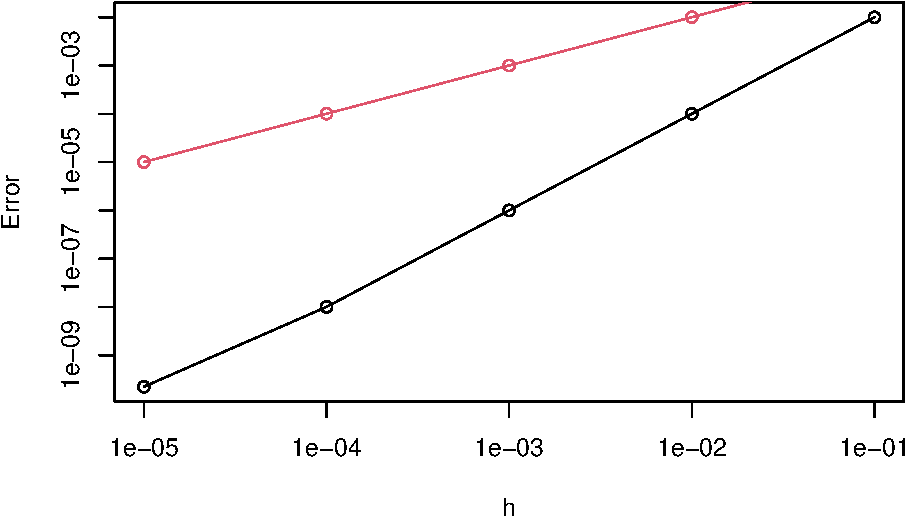
\includegraphics{04-pca_files/figure-latex/unnamed-chunk-10-1.pdf}

R also has a built-in function for doing PCA.

\begin{Shaded}
\begin{Highlighting}[]
\NormalTok{pca <-}\StringTok{ }\KeywordTok{prcomp}\NormalTok{(secondyr[,}\DecValTok{2}\OperatorTok{:}\DecValTok{3}\NormalTok{]) }\CommentTok{# prcomp will automatocally remove the column mean}
\NormalTok{pca}\OperatorTok{$}\NormalTok{rotation }\CommentTok{# the loadings}
\end{Highlighting}
\end{Shaded}

\begin{verbatim}
##            PC1        PC2
## PRB -0.6895160 -0.7242705
## STA -0.7242705  0.6895160
\end{verbatim}

\begin{Shaded}
\begin{Highlighting}[]
\NormalTok{pca}\OperatorTok{$}\NormalTok{x }\CommentTok{# the scores}
\end{Highlighting}
\end{Shaded}

\begin{verbatim}
##              PC1        PC2
##  [1,] -19.060674 -7.2588361
##  [2,] -16.233101 -7.1893271
##  [3,] -11.615016  6.3632849
##  [4,]  14.731183 -0.7695824
##  [5,]  23.074883  5.0940904
##  [6,]  14.939710 -9.2523011
##  [7,]  -3.787059  4.4337549
##  [8,] -29.994240  5.9114764
##  [9,]  15.316435  4.1960474
## [10,]  12.627880 -1.5286074
\end{verbatim}

Note that the new variables have sample mean \(\bar{\mathbf y}=\boldsymbol 0\). The sample covariance matrix is a diagonal with entries given by the eigenvalues (see part 4. of Proposition \ref{prp:pca1}). Note that there is always some numerical error (so quantities are never 0, and instead are just very small numnbers).

\[
\boldsymbol \Lambda= \text{diag}(\lambda_1,\lambda_2) =  \begin{pmatrix} \lambda_1 & 0 \\ 0 & \lambda_2 \end{pmatrix}.
\]

\begin{Shaded}
\begin{Highlighting}[]
\KeywordTok{colMeans}\NormalTok{(pca}\OperatorTok{$}\NormalTok{x)}
\end{Highlighting}
\end{Shaded}

\begin{verbatim}
##           PC1           PC2 
##  2.842171e-15 -9.769963e-16
\end{verbatim}

\begin{Shaded}
\begin{Highlighting}[]
\KeywordTok{cov}\NormalTok{(pca}\OperatorTok{$}\NormalTok{x)}\OperatorTok{*}\DecValTok{9}\OperatorTok{/}\DecValTok{10} \CommentTok{# to convert to using 1/n as the denominator }
\end{Highlighting}
\end{Shaded}

\begin{verbatim}
##              PC1          PC2
## PC1 3.042437e+02 1.974167e-14
## PC2 1.974167e-14 3.315628e+01
\end{verbatim}

Finally, note that we did the singular value decomposition for \(\mathbf X\) above not \(\frac{1}{\sqrt{10}}\mathbf X\), and so we'd need to square and scale the singular values to find the eigenvalues. Let's check:

\begin{Shaded}
\begin{Highlighting}[]
\NormalTok{X_svd}\OperatorTok{$}\NormalTok{d}\OperatorTok{^}\DecValTok{2}\OperatorTok{/}\DecValTok{10} \CommentTok{# square and scale the singular values}
\end{Highlighting}
\end{Shaded}

\begin{verbatim}
## [1] 304.24372  33.15628
\end{verbatim}

\begin{Shaded}
\begin{Highlighting}[]
\KeywordTok{eigen}\NormalTok{(}\KeywordTok{t}\NormalTok{(X) }\OperatorTok\StringTok{ }\NormalTok{X}\OperatorTok{/}\DecValTok{10}\NormalTok{)}\OperatorTok{$}\NormalTok{values  }\CommentTok{# compute the eigenvalues of the covariance matrix}
\end{Highlighting}
\end{Shaded}

\begin{verbatim}
## [1] 304.24372  33.15628
\end{verbatim}

\begin{Shaded}
\begin{Highlighting}[]
\KeywordTok{svd}\NormalTok{(X}\OperatorTok{/}\KeywordTok{sqrt}\NormalTok{(}\DecValTok{10}\NormalTok{))}\OperatorTok{$}\NormalTok{d}\OperatorTok{^}\DecValTok{2} \CommentTok{# compute the singular values of X/sqrt(10) and square}
\end{Highlighting}
\end{Shaded}

\begin{verbatim}
## [1] 304.24372  33.15628
\end{verbatim}

\hypertarget{example-iris}{%
\subsection{Example: Iris}\label{example-iris}}

In general when using R to do PCA, we don't need to compute the SVD and then do the projections, as there is an R command \texttt{prcomp} that will do it all for us. The \texttt{princomp} will also do PCA, but is less stable than \texttt{prcomp}, and it is recommended that you use \texttt{prcomp} in preference.

Let's do PCA on the iris dataset discussed in Chapter \ref{stat-prelim}. The \texttt{prcomp} returns the square root of the eigenvalues (the standard devaiation of the PC scores), and the PC scores.

\begin{Shaded}
\begin{Highlighting}[]
\NormalTok{iris.pca =}\StringTok{ }\KeywordTok{prcomp}\NormalTok{(iris[,}\DecValTok{1}\OperatorTok{:}\DecValTok{4}\NormalTok{])}
\NormalTok{iris.pca}\OperatorTok{$}\NormalTok{sdev }\CommentTok{# the square root of the eigenvalues}
\end{Highlighting}
\end{Shaded}

\begin{verbatim}
## [1] 2.0562689 0.4926162 0.2796596 0.1543862
\end{verbatim}

\begin{Shaded}
\begin{Highlighting}[]
\KeywordTok{head}\NormalTok{(iris.pca}\OperatorTok{$}\NormalTok{x)  }\CommentTok{#the PC scores}
\end{Highlighting}
\end{Shaded}

\begin{verbatim}
##            PC1        PC2         PC3          PC4
## [1,] -2.684126 -0.3193972  0.02791483  0.002262437
## [2,] -2.714142  0.1770012  0.21046427  0.099026550
## [3,] -2.888991  0.1449494 -0.01790026  0.019968390
## [4,] -2.745343  0.3182990 -0.03155937 -0.075575817
## [5,] -2.728717 -0.3267545 -0.09007924 -0.061258593
## [6,] -2.280860 -0.7413304 -0.16867766 -0.024200858
\end{verbatim}

The PC loadings/eigenvectors can also be accessed, as can the sample mean

\begin{Shaded}
\begin{Highlighting}[]
\NormalTok{iris.pca}\OperatorTok{$}\NormalTok{rotation }\CommentTok{#the eigenvecstors}
\end{Highlighting}
\end{Shaded}

\begin{verbatim}
##                      PC1         PC2         PC3        PC4
## Sepal.Length  0.36138659 -0.65658877  0.58202985  0.3154872
## Sepal.Width  -0.08452251 -0.73016143 -0.59791083 -0.3197231
## Petal.Length  0.85667061  0.17337266 -0.07623608 -0.4798390
## Petal.Width   0.35828920  0.07548102 -0.54583143  0.7536574
\end{verbatim}

\begin{Shaded}
\begin{Highlighting}[]
\NormalTok{iris.pca}\OperatorTok{$}\NormalTok{center }\CommentTok{# the sample mean of the data}
\end{Highlighting}
\end{Shaded}

\begin{verbatim}
## Sepal.Length  Sepal.Width Petal.Length  Petal.Width 
##     5.843333     3.057333     3.758000     1.199333
\end{verbatim}

A scree plot can be obtained simply by using the \texttt{plot} command. The summary command also gives useful information about the importance of each PC.

\begin{Shaded}
\begin{Highlighting}[]
\KeywordTok{plot}\NormalTok{(iris.pca)}
\end{Highlighting}
\end{Shaded}

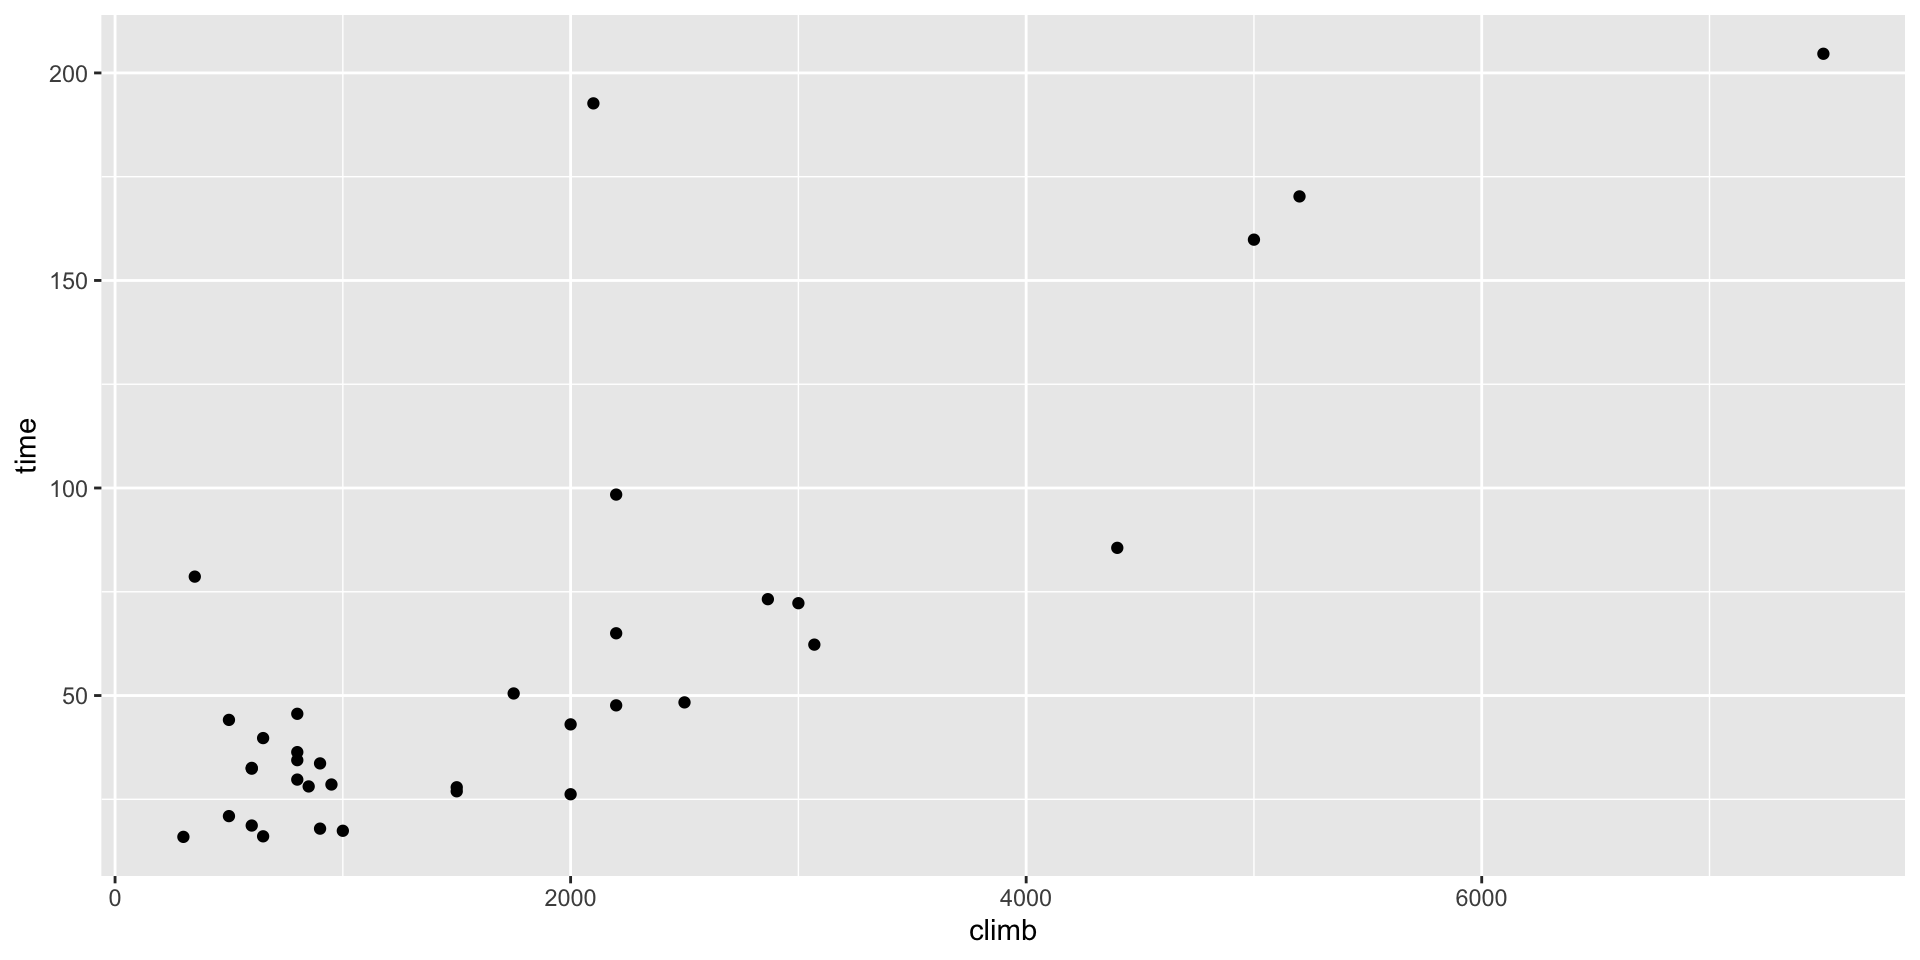
\includegraphics{04-pca_files/figure-latex/unnamed-chunk-16-1.pdf}

\begin{Shaded}
\begin{Highlighting}[]
\KeywordTok{summary}\NormalTok{(iris.pca)}
\end{Highlighting}
\end{Shaded}

\begin{verbatim}
## Importance of components:
##                           PC1     PC2    PC3     PC4
## Standard deviation     2.0563 0.49262 0.2797 0.15439
## Proportion of Variance 0.9246 0.05307 0.0171 0.00521
## Cumulative Proportion  0.9246 0.97769 0.9948 1.00000
\end{verbatim}

To plot the PC scores, you can either manually create a plot or use the \texttt{ggfortify} package. For example, here is a plot of the first two PC scores coloured according to the species of iris.

\begin{Shaded}
\begin{Highlighting}[]
\NormalTok{iris}\OperatorTok{$}\NormalTok{PC1=iris.pca}\OperatorTok{$}\NormalTok{x[,}\DecValTok{1}\NormalTok{]}
\NormalTok{iris}\OperatorTok{$}\NormalTok{PC2=iris.pca}\OperatorTok{$}\NormalTok{x[,}\DecValTok{2}\NormalTok{]}
\KeywordTok{qplot}\NormalTok{(PC1, PC2, }\DataTypeTok{colour=}\NormalTok{Species, }\DataTypeTok{data=}\NormalTok{iris)}
\end{Highlighting}
\end{Shaded}

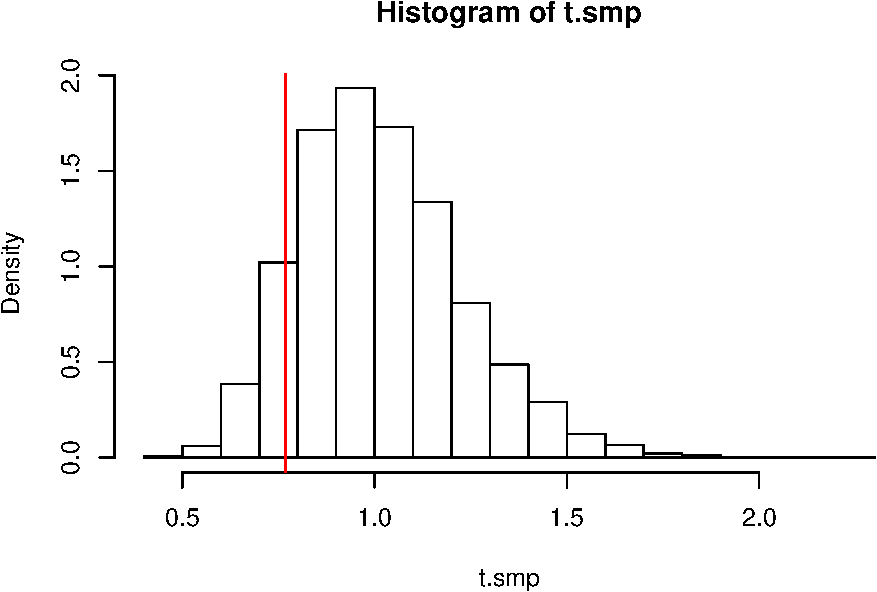
\includegraphics{04-pca_files/figure-latex/unnamed-chunk-17-1.pdf}

The \texttt{ggfortify} package provides a nice wrapper for some of this functionality.

\begin{Shaded}
\begin{Highlighting}[]
\KeywordTok{library}\NormalTok{(ggfortify)}
\KeywordTok{autoplot}\NormalTok{(iris.pca, }\DataTypeTok{data =}\NormalTok{ iris, }\DataTypeTok{colour =} \StringTok{'Species'}\NormalTok{)}
\end{Highlighting}
\end{Shaded}

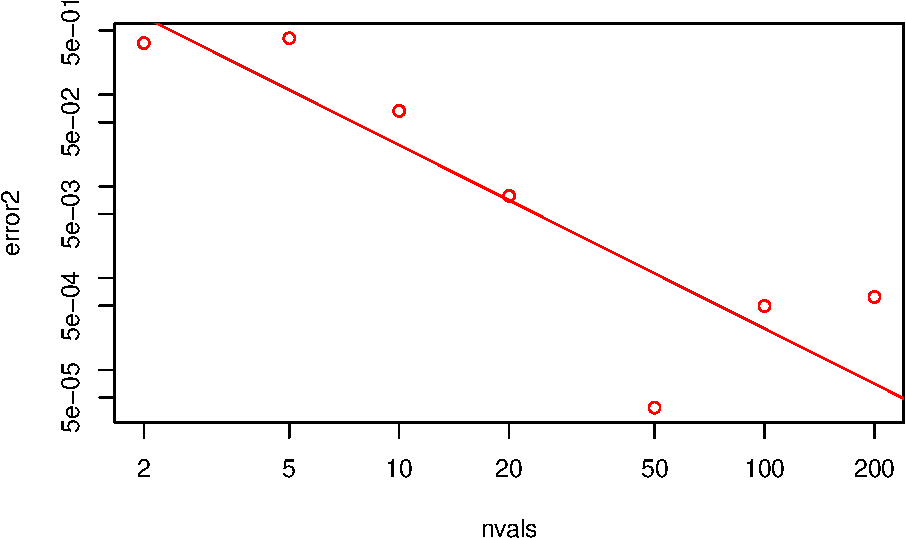
\includegraphics{04-pca_files/figure-latex/unnamed-chunk-18-1.pdf}

\hypertarget{pca-a-formal-description-with-proofs}{%
\section{PCA: a formal description with proofs}\label{pca-a-formal-description-with-proofs}}

Let's now summarize what we've said so far and prove some results about principal component analysis.

Let \(\mathbf x_1, \ldots , \mathbf x_n\) denote a sample of vectors in \(\mathbb{R}^p\) with sample mean vector \(\bar{\mathbf x}\) and sample covariance matrix \(\mathbf S\). Suppose \(\mathbf S=\mathbf X^\top \mathbf H\mathbf X\) has spectral decomposition (see Proposition \ref{prp:spectraldecomp})
\begin{equation}
\mathbf S=\mathbf V\boldsymbol \Lambda\mathbf V^\top = \sum_{j=1}^p  \lambda_j \mathbf v_j \mathbf v_j^\top,
\label{eq:pcaspect}
\end{equation}
where the eigenvalues are \(\lambda_1 \geq \lambda_2 \geq \lambda_p \geq 0\) with \(\boldsymbol \Lambda=\text{diag}\{\lambda_1, \ldots, \lambda_p\}\), and \(\mathbf V\) contains the eigenvectors of \(\mathbf S\).

The principal components of \(\mathbf X\) are defined sequentially. If the \(\mathbf v_k\) is value of \(\mathbf u\) that maximizes the objective for the \(k^{th}\) problem (for \(k<j\)), then the \(j^{th}\) principal component is the solution to the following optimization problem:
\begin{equation}
\max_{\mathbf u: \, \vert \vert \mathbf u\vert \vert =1}\mathbf u^\top \mathbf S\mathbf u
\label{eq:pcmaxgen}
\end{equation}
subject to
\begin{equation}
\mathbf v_k^\top \mathbf u=0, \qquad k=1, \ldots , j-1.
\label{eq:pccongen}
\end{equation}
(for \(j=1\) there is no orthogonality constraint).

\begin{proposition}
\protect\hypertarget{prp:pca1}{}{\label{prp:pca1} }The maximum of Equation \eqref{eq:pcmaxgen}
subject to Equation \eqref{eq:pccongen} is equal to \(\lambda_j\) and is obtained when \(\mathbf u=\mathbf v_j\).
\end{proposition}

\begin{proof}
\iffalse{} {Proof. } \fi{}We can prove this using the method of Lagrange multipliers. For \(j=1\) our objective is
\[\mathcal{L} = \mathbf u^\top  \mathbf S\mathbf u+\lambda(1-\mathbf u^\top \mathbf u)\]
Differentiating (see \ref{vectordiff}) with respect to \(\mathbf u\) and setting the derivative equal to zero gives
\[2\mathbf S\mathbf u-2\lambda \mathbf u=0\]
Rearranging we see that \(\mathbf u\) must satify
\[\mathbf S\mathbf u=\lambda \mathbf u\mbox{ with } \mathbf u^\top \mathbf u=1\]
i.e., \(\mathbf u\) is a unit eigenvector of \(\mathbf S\). Substituting this back in to the objective we see
\[\mathbf u\mathbf S\mathbf u= \lambda\]
and so we must choose \(\mathbf u=\mathbf v_1\), the eigenvector corresponding to the largest eigenvalue of \(\mathbf S\).

We now proceed inductively and assume the result is true for \(k=1, \ldots, j-1\). The Lagrangian for the \(j^{th}\) optimization problem is
\[\mathcal{L} = \mathbf u^\top  \mathbf S\mathbf u+\lambda(1-\mathbf u^\top \mathbf u) +\sum_{k=1}^{j-1}\mu_k (0-\mathbf u^\top \mathbf v_k)\]
where we now have \(j\) Lagrange multipliers \(\lambda, \mu_1, \ldots, \mu_{j-1}\) - one for each constraint.
Differentiating with respect to \(\mathbf u\) and setting equal to zero gives
\[0 = 2\mathbf S\mathbf u- 2\lambda \mathbf u- \sum_{k=1}^{j-1} \mu_k\mathbf v_k=0 \]
If we left multiply by \(\mathbf v_l\) we get
\[2\mathbf v_l^\top \mathbf S\mathbf u- \lambda \mathbf v_l \mathbf u- \sum \mu_k \mathbf v_l^\top \mathbf v_k =0\]
We know \(\mathbf v_l\) is an eigenvector of \(\mathbf S\) and so \(\mathbf S\mathbf v_l=\lambda_l \mathbf v_l\) and hence \(\mathbf v_k \mathbf S\mathbf u=0\) as \(\mathbf v_l^\top \mathbf u=0\). Also \[\mathbf v_l^\top\mathbf v_k=\begin{cases}1 &\mbox{ if } k=l\\
0 &\mbox{ otherwise, }\end{cases}\] and thus we've shown that \(\mu_l=0\) for \(l=1, \ldots, j-1\). So again we have that \[\mathbf S\mathbf u= \lambda \mathbf u\]
i.e., \(\mathbf u\) must be a unit eigenvector of \(\mathbf S\). It only remains to show \emph{which} eigenvector it is. Because \(\mathbf u\) must be orthogonal to \(\mathbf v_1, \ldots, \mathbf v_{j-1}\),
and as \(\mathbf v_l^\top \mathbf S\mathbf v_l = \lambda_l\), we must choose \(\mathbf u=\mathbf v_j\), the eigenvector corresponding to the \(j^{th}\) largest eigenvalue.
\end{proof}

\hypertarget{properties-of-principal-components}{%
\subsection{Properties of principal components}\label{properties-of-principal-components}}

For \(j=1, \ldots , p\), the scores of the \(j^{th}\) principal component (PC) are given by
\[
y_{ij}=\mathbf v_j^\top(\mathbf x_i - \bar{\mathbf x}), \qquad i=1, \ldots , n.
\]
The \(j^{th}\) eigenvector \(\mathbf v_j\) is sometimes referred to as the vector of \textbf{loadings} for the \(j^{th}\) PC.

In vector notation
\[
\mathbf y_i=( y_{i1}, y_{i2}, \ldots , y_{ip})^\top = \mathbf V^\top (\mathbf x_i -\bar{\mathbf x}), \qquad i=1, \ldots ,n.
\]
In matrix form, the full set of PC scores is given by
\[
\mathbf Y= [\mathbf y_1 , \ldots , \mathbf y_n]^\top =\mathbf H\mathbf X\mathbf V.
\]

If \(\tilde{\mathbf X}=\mathbf H\mathbf X\) is the column centered data matrix, with singular value decomposition
\(\tilde{\mathbf X}=\mathbf U\boldsymbol{\Sigma}\mathbf V^\top\) with \(\mathbf V\) as in Equation \eqref{eq:pcaspect}, then
\[\mathbf Y= \tilde{\mathbf X}\mathbf V= \mathbf U\boldsymbol{\Sigma}.\]

The transformed variables \(\mathbf Y= \mathbf H\mathbf X\mathbf V\) have some important properties which we collect together in the following proposition.

\begin{proposition}
\protect\hypertarget{prp:pca2}{}{\label{prp:pca2} }The following results hold:

\begin{enumerate}
\def\labelenumi{\arabic{enumi}.}
\item
  The sample mean vector of \(\mathbf y_1, \ldots , \mathbf y_n\) is the zero vector: \(\bar{\mathbf y}={\mathbf 0}_p\)
\item
  The sample covariance matrix of \(\mathbf y_1, \ldots, \mathbf y_n\) is
  \[\Lambda = \operatorname{diag}(\lambda_1, \ldots, \lambda_p)\]
  i.e., for each fixed \(j\), the sample variance of \(y_{ij}\) is \(\lambda_j\), and \(y_{ij}\) is uncorrelated with with \(y_{ik}\) for \(j\not = k\).
\item
  For \(j\leq k\) the sample variance of \(\{y_{ij}\}_{i=1, \ldots , n}\) is greater than or equal to the sample variance of \(\{y_{ik}\}_{i=1, \ldots , n}\).
  \[\mathbf q_1^\top \mathbf S\mathbf q_1 \geq \mathbf q_2^\top \mathbf S\mathbf q_2 \geq \ldots \geq \mathbf q_p^\top \mathbf S\mathbf q_p\geq 0\]
\item
  The sum of the sample variances is equal to the trace of \(\mathbf S\)
  \[\sum_{j=1}^p \mathbf q_j^\top \mathbf S\mathbf q_j = \sum_{j=1}^p \lambda_j = \text{tr}(\mathbf S)\]
\item
  The product of the sample variances is equal to the determinant of \(\mathbf S\)
  \[\prod_{j=1}^p \mathbf q_j^\top \mathbf S\mathbf q_j = \prod_{j=1}^p \lambda_j = |\mathbf S|.\]
\end{enumerate}
\end{proposition}

\begin{proof}
\iffalse{} {Proof. } \fi{}For i.
\[\bar{\mathbf y} = \frac{1}{n}\sum_{i=1}^n \mathbf V^\top(\mathbf x_i-\bar{\mathbf x}) = \frac{1}{n} \mathbf V^\top\sum_{i=1}^n(\mathbf x_i-\bar{\mathbf x}) =\boldsymbol 0.\]

For 2. the sample covariance matrix of \(\mathbf y_1, \ldots, \mathbf y_n\) is
\begin{align*}
\frac{1}{n}\sum_{i=1}^n \mathbf y_i \mathbf y_i^\top &=\frac{1}{n} \sum \mathbf V^\top (\mathbf x_i-\bar{\mathbf x})(\mathbf x_i - \mathbf x)^\top \mathbf V\\
&=\mathbf V^\top \mathbf S\mathbf V\\
&=\mathbf V^\top \mathbf V\boldsymbol \Lambda\mathbf V^\top \mathbf V\mbox{ substiting the spectral decomposition for }\mathbf S\\
&=\boldsymbol \Lambda
\end{align*}

\begin{enumerate}
\def\labelenumi{\arabic{enumi}.}
\setcounter{enumi}{2}
\item
  is a consequence 2. and of ordering the eigenvalues in decreasing magnitude.
\item
  follows from lemma \ref{lem:trace} and the spectral decomposition of \(\mathbf S\):
  \[\operatorname{tr}(\mathbf S) = \operatorname{tr}(\mathbf V\boldsymbol \Lambda\mathbf V^\top)  =\operatorname{tr}(\mathbf V^\top \mathbf V\boldsymbol \Lambda)=\operatorname{tr}(\boldsymbol \Lambda)=\sum\lambda_i\]
\item
  follows from \ref{prp:deteig}.
\end{enumerate}
\end{proof}

From these properties we say that a proportion
\[\frac{\lambda_j}{\lambda_1 + \ldots + \lambda_p}\]
of the variability in the sample is `explained' by the \(j^{th}\) PC.

One tool for looking at the contributions of each PC is to look at the \textbf{scree plot} which plots the percentage of variance explained by PC \(j\) against \(j\). We'll see examples of scree plots below.

\hypertarget{pca:football}{%
\subsection{Example: Football}\label{pca:football}}

We can apply PCA to a football league table where \(W\), \(D\), \(L\) are the number of matches won, drawn and lost and \(G\) and \(GA\) are the goals scored for and against, and \(GD\) is the goal difference (\(G-GA\)). An extract of the table for the 2019-2020 Premier League season is:

\begin{tabular}{lrrrrrr}
\toprule
Team & W & D & L & G & GA & GD\\
\midrule
Liverpool & 32 & 3 & 3 & 85 & 33 & 52\\
Manchester City & 26 & 3 & 9 & 102 & 35 & 67\\
Manchester United & 18 & 12 & 8 & 66 & 36 & 30\\
Chelsea & 20 & 6 & 12 & 69 & 54 & 15\\
Leicester City & 18 & 8 & 12 & 67 & 41 & 26\\
\addlinespace
Tottenham Hotspur & 16 & 11 & 11 & 61 & 47 & 14\\
Wolverhampton & 15 & 14 & 9 & 51 & 40 & 11\\
Arsenal & 14 & 14 & 10 & 56 & 48 & 8\\
Sheffield United & 14 & 12 & 12 & 39 & 39 & 0\\
Burnley & 15 & 9 & 14 & 43 & 50 & -7\\
\bottomrule
\end{tabular}

The sample mean vector is

\[\bar{\mathbf x} =\begin{pmatrix}14.4 \\9.2 \\14.4 \\51.7 \\51.7 \\0 \\\end{pmatrix}.\]

Note that the total goals scored must equal the total goals conceded, and that the sum of the goal differences must be \(0\). The sample covariance matrix is

\begin{equation}
\mathbf S= \begin{pmatrix}38.3&-9.18&-29.2&103&-57&160 \\-9.18&10.2&-0.98&-27.5&-2.24&-25.2 \\-29.2&-0.98&30.1&-75.3&59.3&-135 \\103&-27.5&-75.3&336&-147&483 \\-57&-2.24&59.3&-147&134&-281 \\160&-25.2&-135&483&-281&764 \\\end{pmatrix}
\label{eq:PLES}
\end{equation}

The eigenvalues of \(\mathbf S\) are
\[\boldsymbol \Lambda= \text{diag}\begin{pmatrix}1300&71.9&8.05&4.62&-2.65e-14&-3.73e-14 \\\end{pmatrix}\]

Note that we have two zero eigenvalues (which won't be computed as exactly zero because of numerical rounding errors) because two of our variables are a linear combinations of the other variables, \(W+D+L = 38\) and \(GD=G-GA\). The corresponding eigenvectors are
\[\mathbf V= [\mathbf v_1 \ldots \mathbf v_6] =\begin{pmatrix}-0.166&0.0262&-0.707&0.373&0.222&-0.533 \\0.0282&-0.275&0.661&0.391&0.222&-0.533 \\0.138&0.249&0.0455&-0.764&0.222&-0.533 \\-0.502&0.6&0.202&0.117&0.533&0.222 \\0.285&0.701&0.11&0.286&-0.533&-0.222 \\-0.787&-0.101&0.0915&-0.169&-0.533&-0.222 \\\end{pmatrix}\]

The proportion of variability explained by each of the PCs is:
\[
\begin{pmatrix}0.939&0.052&0.00583&0.00334&-1.92e-17&-2.7e-17 \\\end{pmatrix}
\]

There is no point computing the scores for PC 5 and 6, because these do not explain any of the variability in the data. Similarly, there is little value in computing the scores for PCs 3 \& 4 because they account for less than 1\% of the variability in the data.

We can, therefore, choose to compute only the first two PC scores. We are reducing the dimension of our data set from \(p=5\) to \(p=2\) while still retaining 99\% of the variability. The first PC score/transformed variable is given by:
\begin{align*}
y_{i1} &= -0.17(W_i-\bar{W}) +0.03(D_i-\bar{D}) +0.14(L_i-\bar{L})\\
& \qquad +-0.5(G_i-\bar{G}) +0.28(GA_i-\bar{GA})+-0.79(GD_i-\bar{GD}),
\end{align*}
and similarly for PC 2.

The first five rows of our revised `league table' are now

\begin{table}[H]
\centering
\begin{tabular}{lrr}
\toprule
Team & PC1 & PC2\\
\midrule
Liverpool & -67.6 & 0.9\\
Manchester City & -85.6 & 12.3\\
Manchester United & -36.7 & -7.7\\
Chelsea & -21.2 & 10.9\\
Leicester City & -32.2 & -1.1\\
\bottomrule
\end{tabular}
\end{table}

Now that we have reduced the dimension to \(p=2\), we can visualise the differences between the teams.

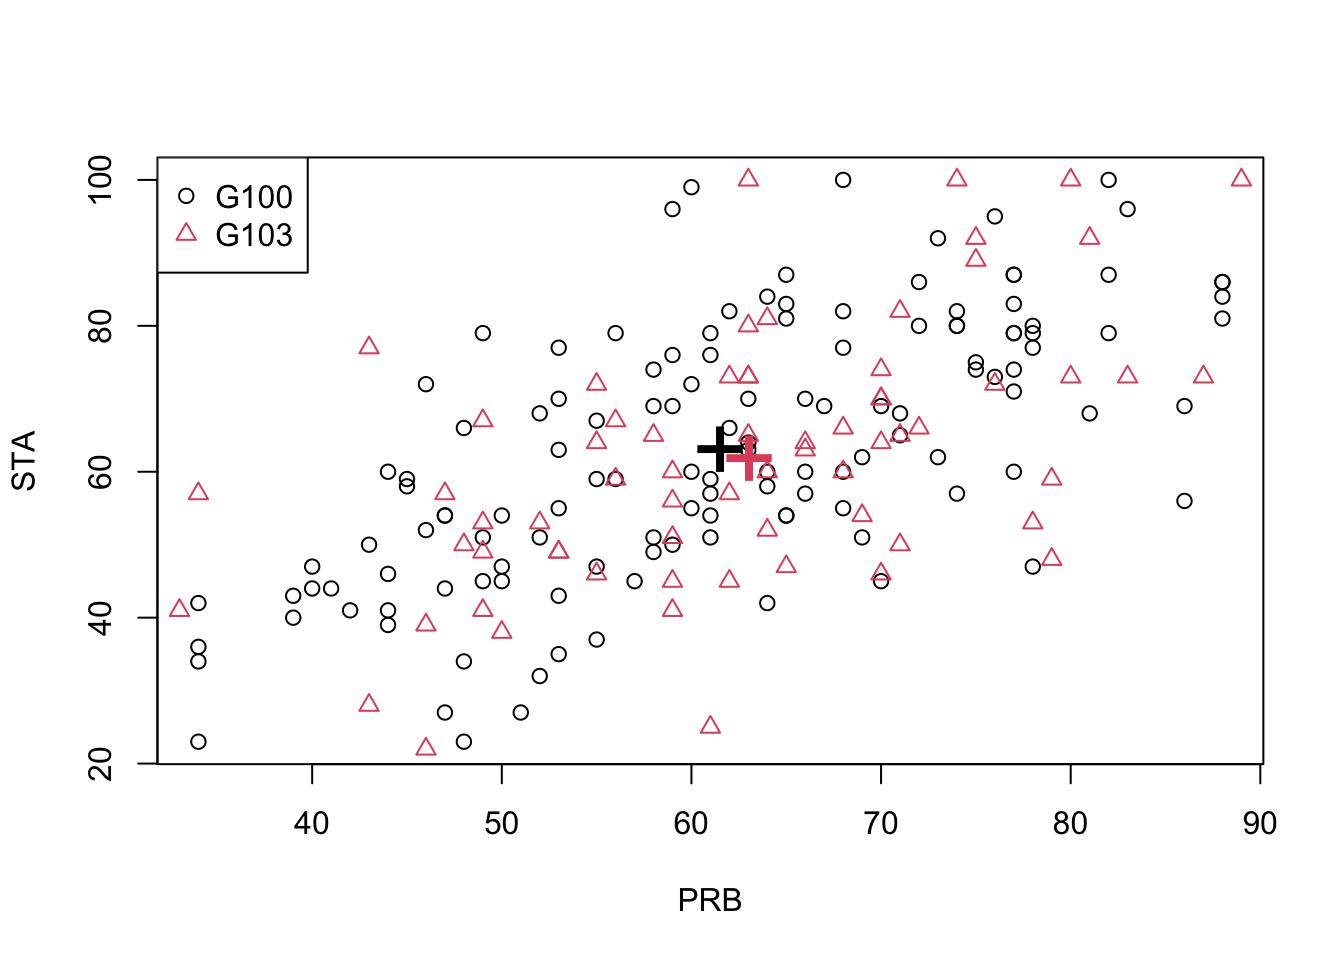
\includegraphics{04-pca_files/figure-latex/unnamed-chunk-26-1.pdf}

We might interpret the PCs as follows. The first PC seems to measure the difference in goals scored and conceded between teams. Low values of PC1 indicate good peformance, and high values poor performance. Teams are rewarded with -0.79 for each positive goal difference, and -0.5 for each goal scored, whilst being penalised by 0.28 for every goal they concede. So a team with a large negative positive PC1 score tends to score lots of goals and concede few. If we rank teams by their PC1 score, and compare this with the rankings using 3 points for a win and 1 point for a draw we get a different ranking of the teams.

\begin{tabular}{lrr}
\toprule
  & PC1 & PC2\\
\midrule
Manchester City & -85.59 & 12.35\\
Liverpool & -67.64 & 0.93\\
Manchester United & -36.66 & -7.73\\
Leicester City & -32.16 & -1.13\\
Chelsea & -21.19 & 10.90\\
\bottomrule
\end{tabular}

The second PC has a strong positive loading for both goals for and against. A team with a large positive PC 2 score was, therefore, involved in matches with lots of goals. We could, therefore, interpret PC 2 as an `entertainment' measure, ranking teams according to their involvement in high-scoring games.

The above example raises the question of how many PCs should we use in practice. If we reduce the dimension to \(p=1\) then we can rank observations and analyse our new variable with univariate statistics. If we reduce the dimension to \(p=2\) then it is still easy to visualise the data. However, reducing the dimension to \(p=1\) or \(p=2\) may involve losing lots of information and a sensible answer should depend on the objectives of the analysis and the data itself.

The scree graph for the football example is:

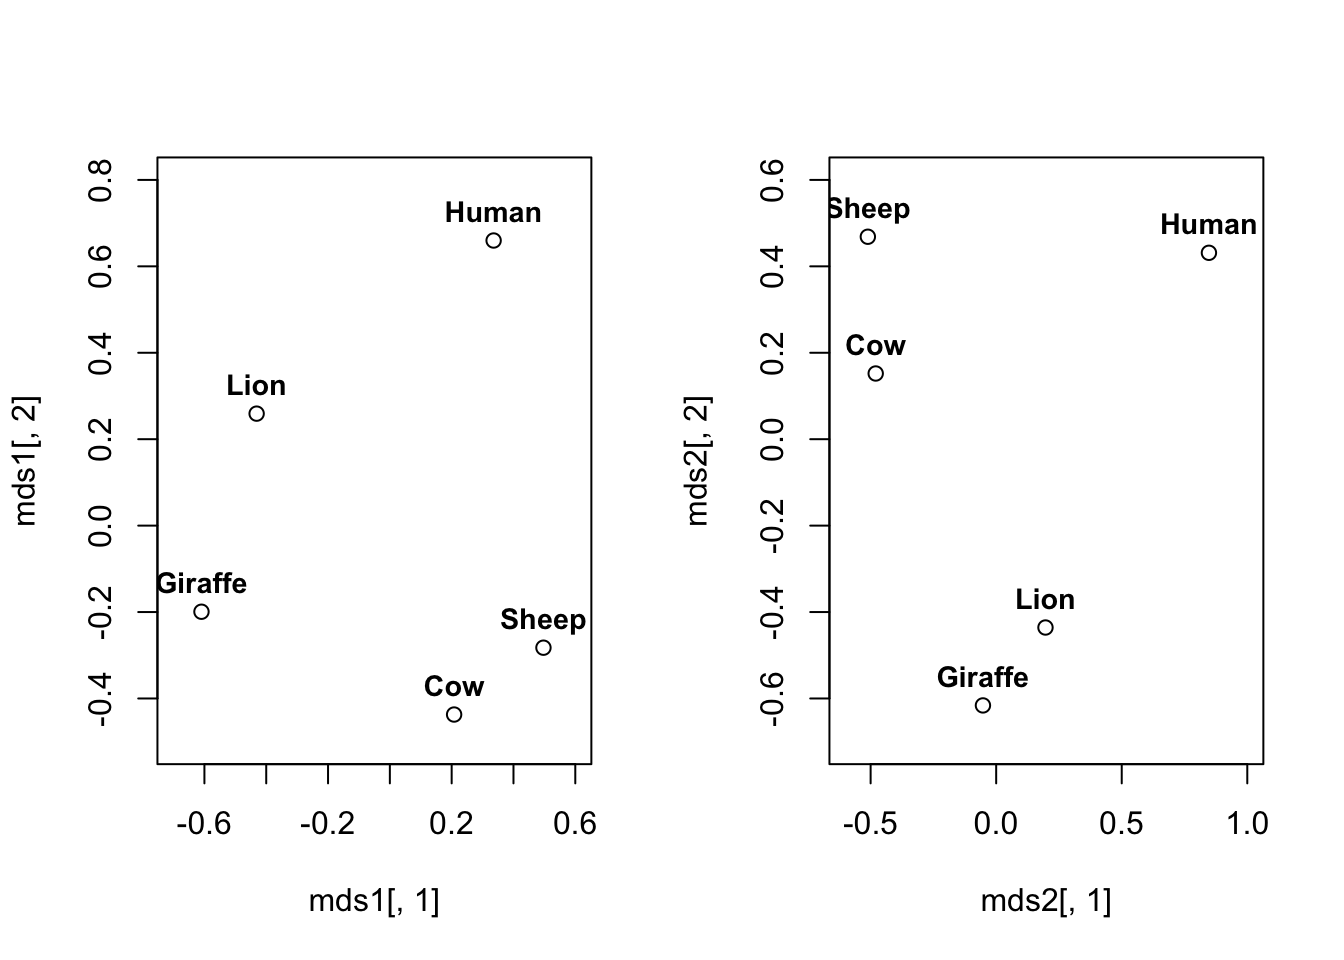
\includegraphics{04-pca_files/figure-latex/unnamed-chunk-29-1.pdf}

There are many possible methods for choosing the number of PCs to retain for analysis, including:

\begin{itemize}
\tightlist
\item
  retaining enough PCs to explain, say, 90\% of the total variation;
\item
  retaining PCs where the eigenvalue is above the average.
\end{itemize}

To retain enough PCs to explain 90\% of the total variance, would require us to keep just a single PCs in this case.

\hypertarget{pcawithR}{%
\subsection{\texorpdfstring{PCA based on \(\mathbf R\) versus PCA based on \(\mathbf S\)}{PCA based on \textbackslash{}mathbf R versus PCA based on \textbackslash{}mathbf S}}\label{pcawithR}}

Recall the distinction between the sample covariance matrix \(\mathbf S\) and the sample correlation matrix \(\mathbf R\).
Note that all correlation matrices are also covariance matrices, but not all covariance matrices are correlation matrices.
Before doing PCA we must decide whether to do PCA based on \(\mathbf S\) or \(\mathbf R\)? As we will see later

\begin{itemize}
\tightlist
\item
  PCA based on \(\mathbf R\) (but not \(\mathbf S\)) is scale invariant, whereas
\item
  PCA based on \(\mathbf S\) is invariant under orthogonal rotation.
\end{itemize}

If the original \(p\) variables represent very different types of quantity or show marked differences in variances, then it will usually be better to use \(\mathbf R\) rather than \(\mathbf S\). However, in some circumstances, we may wish to use \(\mathbf S\), such as when the \(p\) variables are measuring similar entities and the sample variances are not too different.

Given that the required numerical calculations are easy to perform in R, we might wish to do it both ways and see if it makes much difference. To use the correlation matrix \(\mathbf R\), we just add the option \texttt{scale=TRUE} when using the \texttt{prcomp} command.

\hypertarget{football-example-continued}{%
\subsubsection{Football example continued}\label{football-example-continued}}

If we repeat the analysis of the football data using \(\mathbf R\) instead of \(\mathbf S\), we get find principal components:

\begin{align*}
\boldsymbol \Lambda&= \text{diag}\begin{pmatrix}4.51&1.25&0.156&0.0863&3.68e-32&2.48e-33 \\\end{pmatrix}\\
\;\\
\mathbf V= [\mathbf v_1 \ldots \mathbf v_6] &=\begin{pmatrix}-0.456&0.149&-0.342&-0.406&0.466&0.52 \\0.143&-0.844&0.344&-0.143&0.24&0.268 \\0.432&0.321&0.186&0.541&0.413&0.461 \\-0.438&0.214&0.7&-0.0181&0.389&-0.348 \\0.419&0.342&0.386&-0.671&-0.245&0.22 \\-0.466&-0.00136&0.302&0.269&-0.586&0.525 \\\end{pmatrix}
\end{align*}

The effect of using \(\mathbf R\) is to standardize each of the original variables to have variance 1.
The first PC now has loadings which are more evenly balanced across the 6 original variables.

Teams will have a small value of PC1 score if they won lots, lost rarely, scored a lot, and conceded rarely. In other words, PC1 is a complete measure of overall performance. If we look at the league table based on ordering according to PC1 we get a table that looks more like the original table.

\begin{tabular}{lrr}
\toprule
  & PC1 & PC2\\
\midrule
Liverpool & -4.70 & 1.20\\
Manchester City & -4.38 & 1.65\\
Manchester United & -2.01 & -1.29\\
Chelsea & -1.29 & 1.08\\
Leicester City & -1.66 & 0.12\\
\addlinespace
Tottenham Hotspur & -0.91 & -0.65\\
Wolverhampton & -0.82 & -1.88\\
Arsenal & -0.46 & -1.56\\
Sheffield United & -0.18 & -1.38\\
Burnley & 0.18 & -0.10\\
\bottomrule
\end{tabular}

Overall for these data, doing PCA with \(\mathbf R\) instead of \(\mathbf S\) better summarizes the data (although this is just my subjective opinion - you may feel differently).

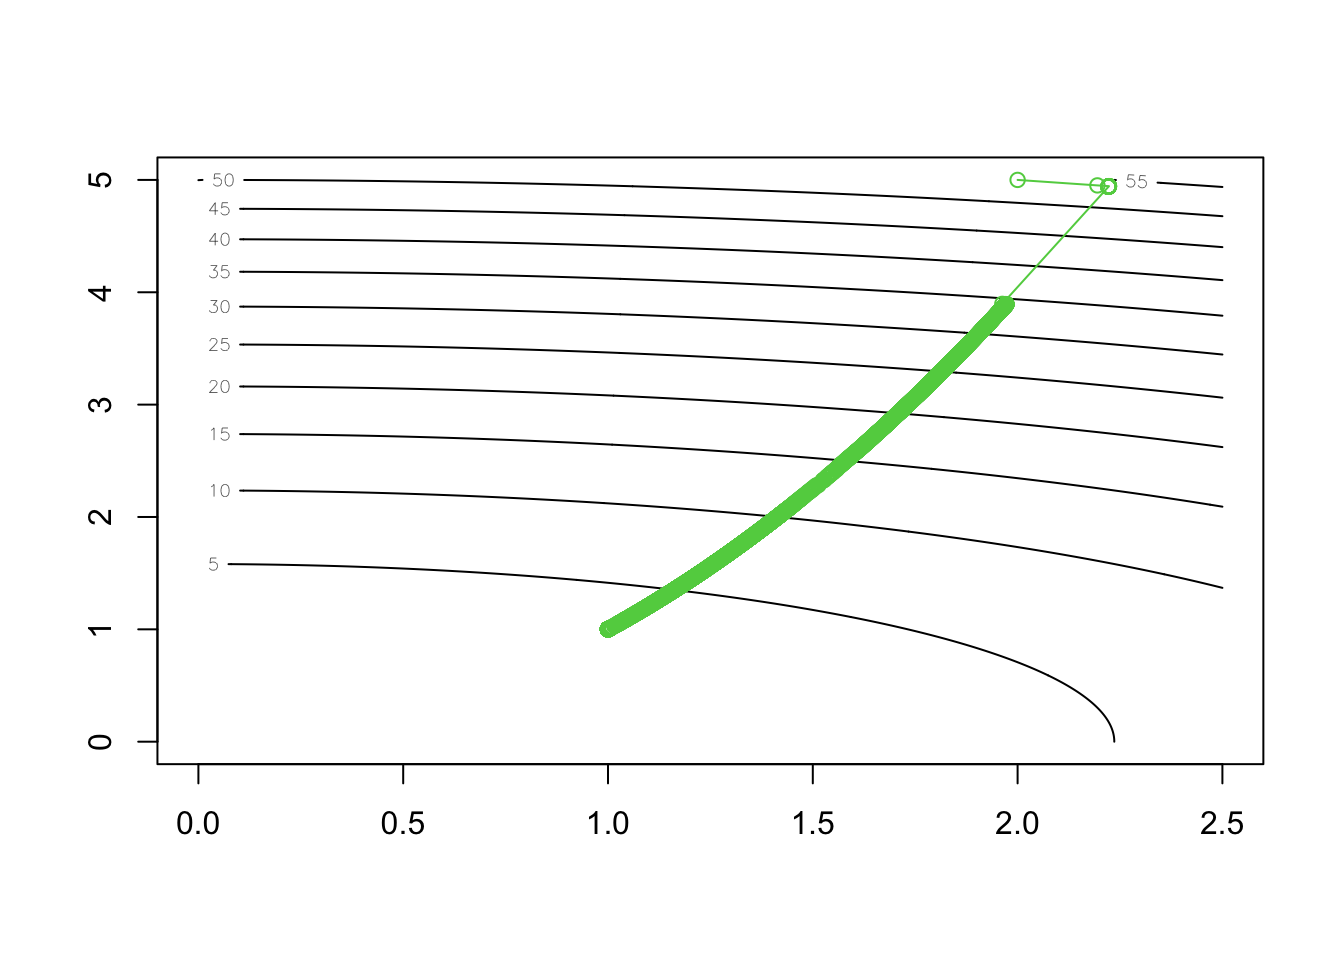
\includegraphics{04-pca_files/figure-latex/unnamed-chunk-32-1.pdf}

\hypertarget{population-pca}{%
\subsection{Population PCA}\label{population-pca}}

So far we have considered sample PCA based on the sample covariance matrix or sample correlation matrix:
\[
\mathbf S=\frac{1}{n}\sum_{i=1}^n (\mathbf x_i-\bar{\mathbf x})(\mathbf x_i-\bar{\mathbf x})^\top.
\]

We note now that there is a \emph{population} analogue of PCA based on the population
covariance matrix \(\boldsymbol{\Sigma}\). Although the population version of PCA is not of as much direct practical
relevance as sample PCA, it is nevertheless of conceptual importance.

Let \(\mathbf x\) denote a \(p \times 1\) random vector with \({\mathbb{E}}(\mathbf x)={\pmb \mu}\) and \({\mathbb{V}\operatorname{ar}}(\mathbf x)={\pmb \Sigma}\). As defined,
\(\pmb \mu\) is the population mean vector and \(\pmb \Sigma\) is the population covariance matrix.

Since \(\pmb \Sigma\) is symmetric, the spectral decomposition theorem tells us that
\[
{\pmb \Sigma}=\sum_{j=1}^p \check{\lambda}_j \check{\mathbf v}_j \check{\mathbf v}_j^\top=\check{\mathbf V} \check{\boldsymbol \Lambda}\check{\mathbf V}^\top
\]
where the `check' symbol \(\quad \check{} \quad\) is used to distinguish population quantities from their sample analogues.

Then:

\begin{itemize}
\tightlist
\item
  the first population PC is defined by \(Y_1=\check{\mathbf v}_1^\top (\mathbf x-{\pmb \mu})\);
\item
  the second population PC is defined by \(Y_2=\check{\mathbf v}_2^\top (\mathbf x-{\pmb \mu})\);
\item
  \(\ldots\)
\item
  the \(p\)th population PC is defined by \(Y_p=\check{\mathbf v}_p^\top (\mathbf x-{\pmb \mu})\).
\end{itemize}

The \(Y_1, \ldots , Y_p\) are random variables, unlike the sample PCA case, where the \(y_{ij}\) are observed quantities.
In the sample PCA case, the \(y_{ij}\) can often be regarded as the observed values of random variables.

In matrix form, the above definitions can be summarised by writing
\[
\mathbf y=\begin{pmatrix} Y_1 \\ Y_2 \\ ... \\...\\Y_p   \end{pmatrix} = \check{\mathbf V}^\top (\mathbf x-{\pmb \mu}).
\]

The population PCA analogues of the sample PCA properties listed in Proposition \ref{prp:pca2} are now given. Note that the
\(Y_j\)'s are random variables as opposed to observed values of random variables.

\begin{proposition}
\protect\hypertarget{prp:pca3}{}{\label{prp:pca3} }The following results hold for the random variables \(Y_1, \ldots , Y_p\) defined above.

\begin{enumerate}
\def\labelenumi{\arabic{enumi}.}
\item
  \({\mathbb{E}}(Y_j)=0\) for \(j=1, \ldots , p\);
\item
  \({\mathbb{V}\operatorname{ar}}(Y_j)=\check{\lambda}_j\) for \(j=1,\ldots, p\);
\item
  \({\mathbb{C}\operatorname{ov}}(Y_j,Y_k)=0\) if \(j \neq k\);
\item
  \({\mathbb{V}\operatorname{ar}}(Y_1) \geq {\mathbb{V}\operatorname{ar}}(Y_2) \geq \cdots \geq {\mathbb{V}\operatorname{ar}}(Y_p) \geq 0\);
\item
  \(\sum_{j=1}^p {\mathbb{V}\operatorname{ar}}(Y_j)=\sum_{j=1}^p \check{\lambda}_j=\text{tr}(\boldsymbol{\Sigma})\);
\item
  \(\prod_{j=1}^p \text{Var}(Y_j)=\prod_{j=1}^p \check{\lambda}_j=\vert \boldsymbol{\Sigma}\vert\).
\end{enumerate}
\end{proposition}

Note that, defining \(\mathbf y=(Y_1, \ldots , Y_p)^\top\) as before, part 1. implies that \({\mathbb{E}}(\mathbf y)={\mathbf 0}_p\) and parts 2. and 3. together imply that
\[
\text{Var}(\mathbf y)=\boldsymbol \Lambda\equiv \text{diag}(\check{\lambda}_1, \ldots , \check{\lambda}_p).
\]

Consider now a repeated sampling framework in which we assume that \(\mathbf x_1, \ldots , \mathbf x_n\) are IID random vectors from a population
with mean vector \(\pmb \mu\) and covariance matrix \(\boldsymbol{\Sigma}\).

What is the relationship between the sample PCA based on the sample of observed vectors \(\mathbf x_1, \ldots , \mathbf x_n\), and the population PCA based on the unobserved random vector \(\mathbf x\),
from the same population?

If the elements of \(\boldsymbol{\Sigma}\) are all finite, then as \(n\) increases, the elements of the sample covariance matrix \(\mathbf S\) will converge to the corresponding elements
of the population covariance matrix \(\boldsymbol{\Sigma}\). Consequently, we expect the principal components from sample PCA to converge to the population PCA values as \(n\) grows large. Justification of this statement comes from the weak law of large numbers applied to the components of \(\Sigma\), but the details are beyond the scope of this module.

\hypertarget{pca-under-transformations-of-variables}{%
\subsection{PCA under transformations of variables}\label{pca-under-transformations-of-variables}}

We'll now consider what happens to PCA when the data are transformed in various ways.

\textbf{Addition transformation}

Firstly, consider the transformation of addition where, for example, we add a fixed amount to each variable.
We can write this transformation as \(\mathbf z_i = \mathbf x_i + \mathbf c\), where \(\mathbf c\) is a fixed vector. Under this transformation the sample mean changes, \(\bar{\mathbf z} = \bar{\mathbf x} + \mathbf c\), but the sample variance remains \(\mathbf S\). Consequently, the eigenvalues and eigenvectors remain the same and, therefore, so do the principal component scores/transformed vasriables,
\[\mathbf y_i = \mathbf V^\top (\mathbf z_i - \bar{\mathbf z}) = \mathbf V^\top(\mathbf x_i + \mathbf c- (\bar{\mathbf x} + \mathbf c)) = \mathbf V^\top (\mathbf x_i - \bar{\mathbf x}).\]
We say that the principal components are \textbf{invariant} under the addition transformation. An important special case is to choose \(\mathbf c= -\bar{\mathbf x}\) so that the PC scores are simply \(\mathbf y_i = \mathbf V^\top \mathbf z_i\).

\textbf{Scale transformation}

Secondly, we consider the scale transformation where each variable is multiplied by a fixed amount.
A scale transformation occurs more naturally when we convert units of measurement from, say, metres to kilometres. We can write this transformation as \(\mathbf z_i = \mathbf D\mathbf x_i\), where \(\mathbf D\) is a diagonal matrix with positive elements. Under this transformation the sample mean changes from \(\bar{\mathbf x}\) to \(\bar{\mathbf z} = \mathbf D\bar{\mathbf x}\), and the sample covariance matrix changes from \(\mathbf S\) to \(\mathbf D\mathbf S\mathbf D\). Consequently, the principal components also change.

This lack of scale-invariance is undesirable. For example, if we analysed data that included some information on distances, we don't want the answer to depend upon whether we use km, metres, or miles as the measure of distance.
One solution is to scale the data using
\[
\mathbf D= \text{diag}(s_{11}^{-1/2}, \ldots , s_{pp}^{-1/2}),
 \]
where \(s_{ii}\) is the \(i\)th diagonal element of \(\mathbf S\). In effect, we have standardised all the new variables to have variance 1. In this case the sample covariance matrix of the \(\mathbf z_i\)'s is simply the sample correlation matrix \(\mathbf R\) of the original variables, \(\mathbf x_i\). Therefore, we can carry out PCA on the sample correlation matrix, \(\mathbf R\), which is invariant to changes of scale.

In summary: \(\mathbf R\) is scale-invariant while \(\mathbf S\) is not. To do PCA on \(\mathbf R\) in R we use the option \texttt{scale=TRUE} in the \texttt{prcomp} command.

We saw an example of this in section \ref{pcawithR} with the football data. Because the sample
variances of \(G\) and \(GA\) are much larger than the sample variances of \(W\), \(D\) and \(L\), doing PCA with \(\mathbf R\) instead of \(\mathbf S\) completely changed the analysis.

\textbf{Orthogonal transformations}

Thirdly, we consider a transformation by an orthogonal matrix, \(\stackrel{p \times p}{\mathbf A}\), such that \(\mathbf A\mathbf A^\top = \mathbf A^\top \mathbf A= \mathbf I_p\), and write \(\mathbf z_i = \mathbf A\mathbf x_i\). This is equivalent to rotating and/or reflecting the original data.

Let \(\mathbf S\) be the sample covariance matrix of the \(\mathbf x_i\) and let \(\mathbf T\) be the sample covariance matrix of the \(\mathbf z_i\). Under this transformation the sample mean changes from \(\bar{\mathbf x}\) to \(\bar{\mathbf z} = \mathbf A\bar{\mathbf x}\), and the sample covariance matrix \(\mathbf S\) changes from \(\mathbf S\) to \(\mathbf T= \mathbf A\mathbf S\mathbf A^\top\).

However, if we write \(\mathbf S\) in terms of its spectral decomposition \(\mathbf S= \mathbf V\boldsymbol \Lambda\mathbf V^\top\), then \(\mathbf T= \mathbf A\mathbf V\boldsymbol \Lambda\mathbf V^\top \mathbf A^\top = \mathbf B\boldsymbol \Lambda\mathbf B^\top\) where \(\mathbf B= \mathbf A\mathbf V\) is also orthogonal. It is therefore apparent that the eigenvalues of \(\mathbf T\) are the same as those of \(\mathbf S\); and the eigenvectors of \(\mathbf T\) are given by \(\mathbf b_j\) where \(\mathbf b_j = \mathbf A\mathbf v_j\), \(j=1,\ldots,p\). The PC scores of the rotated variables are
\[ \mathbf y_i = \mathbf B^\top (\mathbf z_i - \bar{\mathbf z}) = \mathbf V^\top \mathbf A^\top \mathbf A(\mathbf x_i - \bar{\mathbf x}) = \mathbf V_1^\top (\mathbf x_i - \bar{\mathbf x}),\]
and so they are identical to the PC scores of the original variables.

Therefore, under an orthogonal transformation the eigenvalues and PC scores are unchanged; the PCs are orthogonal transformations of the original PCs. We say that the principal components are \textbf{equivariant} with respect to orthogonal transformations.

\hypertarget{an-alternative-view-of-pca}{%
\section{An alternative view of PCA}\label{an-alternative-view-of-pca}}

In this section, we will again consider the situation in which the sample \(\mathbf x_1, \ldots , \mathbf x_n \in \mathbb{R}^p\) have zero mean (replace \(\mathbf x_i\) by \(\mathbf x_i-\bar{\mathbf x}\) if the mean is not zero).

To recap, in PCA to find the \(r\) leading principal components, we solve the optimization problem
\begin{align*}
\mbox{For } k=1, \ldots, r &\mbox{ maximize } \mathbf u_k^\top \mathbf S\mathbf u_k \\
 &\mbox{ subject to } \mathbf u_k^\top \mathbf u_j = \begin{cases}
 1  &\mbox{ if } j=k\\
 0 & \mbox{ otherwise.}
 \end{cases}
 \end{align*}

We can write this in the form given in the introduction to this chapter (Equation \eqref{eq:dimredopt}) as
\begin{align*}
&\mbox{Maximize } \operatorname{tr}(\mathbf U^\top \mathbf S\mathbf U) \\
 &\mbox{ subject to } \mathbf U^\top \mathbf U=\mathbf I_r,
 \end{align*}
as \(\operatorname{tr}(\mathbf U^\top \mathbf S\mathbf U) = \sum_{k=1}^r \mathbf u_k^\top \mathbf S\mathbf u_k\) if \(\mathbf U\) has columns \(\mathbf u_1, \ldots, \mathbf u_r\).

\hypertarget{an-equivalent-problem}{%
\subsubsection*{An equivalent problem}\label{an-equivalent-problem}}
\addcontentsline{toc}{subsubsection}{An equivalent problem}

There is another optimization problem that we sometimes wish to solve, that turns out to be equivalent to the above, thus providing another reason why PCA is so widely used.

Suppose we want to find the best rank-\(r\) linear approximation to the data matrix \(\mathbf X=\begin{pmatrix}\mathbf x_1& \ldots & \mathbf x_n\end{pmatrix}^\top\) (remember that we're assuming the data have been column centered, if not, replace \(\mathbf X\) by \(\mathbf H\mathbf X\)). One way to think about this is seek a \(p\times r\) matrix \(\mathbf U\) for which the rank \(r\) linear model
\[f(\mathbf y) = \mathbf U\mathbf y\] can be used to represent the data.

Let's choose \(\mathbf y_i\in \mathbb{R}^r\) and \(\mathbf U\) to minimize the sum of squared errors
\[\sum_{i=1}^n ||\mathbf x_i - \mathbf U\mathbf y_i||^2_2.\]

If we write
\[\mathbf Y^\top = \begin{pmatrix} 
| &&|\\
\mathbf y_1& \ldots & \mathbf y_n\\
| &&|
\end{pmatrix}\]
then
\begin{align*}
\sum_{i=1}^n ||\mathbf x_i - \mathbf U\mathbf y_i||^2_2 &=\operatorname{tr}((\mathbf X^\top - \mathbf U\mathbf Y^\top)^\top (\mathbf X^\top - \mathbf U\mathbf Y^\top))\\
&=||\mathbf X^\top - \mathbf U\mathbf Y^\top||_F^2
\end{align*}

i.e., we're looking for the rank-\(r\) matrix \(\mathbf X_r\) that minimizes \(||\mathbf X- \mathbf X_r||_F=||\mathbf X^\top - \mathbf X_r^\top||_F\), noting that we can write an arbitrary rank-\(r\) matrix as \(\mathbf X_r^\top = \mathbf U\mathbf Y^\top\) for some \(p\times r\) matrix \(\mathbf U\) and a \(n \times r\) matrix \(\mathbf Y\).

It makes sense to restrict the columns of \(\mathbf U\) to be orthonormal so that \(\mathbf U^\top \mathbf U=\mathbf I_r\) as non-orthonormal coordinates systems are confusing. We know that the \(\mathbf u\in \mathcal{C}(\mathbf U)\) (where \(\mathcal{C}(\mathbf U)\) is the column space of \(\mathbf U\)) that minimizes
\[||\mathbf x-\mathbf u||_2\]
is the orthogonal projection of \(\mathbf x\) onto \(\mathcal{C}(\mathbf U)\), which given the columns of \(\mathbf U\) are orthonormal is \(\mathbf u= \mathbf U\mathbf U^\top \mathbf x\) (see Section \ref{orthogproj}). So we must have \(\mathbf X_r^\top = \mathbf U\mathbf U^\top \mathbf X^\top\) and \(\mathbf Y^\top = \mathbf U^\top \mathbf X^\top\).

So it remains to find the optimal choice for \(\mathbf U\) by minimizing
\begin{align*}
||\mathbf X^\top - \mathbf U\mathbf U^\top \mathbf X^\top||_F &=||\mathbf X- \mathbf X\mathbf U\mathbf U^\top ||_F\\
&= \operatorname{tr}((\mathbf X- \mathbf X\mathbf U\mathbf U^\top)^\top(\mathbf X- \mathbf X\mathbf U\mathbf U^\top))\\
&= \operatorname{tr}(\mathbf X^\top \mathbf X) - 2 \operatorname{tr}(\mathbf U\mathbf U^\top \mathbf X^\top\mathbf X) +  \operatorname{tr}(\mathbf U\mathbf U^\top \mathbf X^\top\mathbf X\mathbf U\mathbf U^\top)\\
&= \operatorname{tr}(\mathbf X^\top \mathbf X)  - \operatorname{tr}(\mathbf U^\top \mathbf X^\top \mathbf X\mathbf U) 
\end{align*}
where we've used the fact \(\operatorname{tr}(\mathbf A\mathbf B) = \operatorname{tr}(\mathbf B\mathbf A)\) and that \(\mathbf U^\top \mathbf U=\mathbf I_r\).

Minimizing the equation above with respect to \(\mathbf U\) is equivalent to maximizing
\[\operatorname{tr}(\mathbf U^\top \mathbf S\mathbf U) \]
which is the maximum variance objective we used to introduce PCA.

So to summarize, the optimization problem
\begin{align*}
&\mbox{Minimize } ||\mathbf X^\top -\mathbf U\mathbf U^\top \mathbf X^\top||_F \\
 &\mbox{ subject to } \mathbf U^\top \mathbf U=\mathbf I_r,
 \end{align*}
is equivalent to (and has the same as) the PCA optimization problem.

\hypertarget{example-mnist-handwritten-digits}{%
\subsection{Example: MNIST handwritten digits}\label{example-mnist-handwritten-digits}}

Let's consider the MNIST dataset of handwritten digits discussed in Chapter \ref{stat-prelim}. Recall this is a collection of 60,000 digits, each of which has been converted to a \(28\times 28\) pixel greyscale image (so \(p=784\)).
I've made a clean version of the dataset available on Moodle, so you can try this analysis for yourself. Let's look at just the 3s. I've created a plotting function \texttt{plot.mnist}, which is in the code file on Moodle.

\begin{Shaded}
\begin{Highlighting}[]
\KeywordTok{load}\NormalTok{(}\DataTypeTok{file=}\StringTok{"mnist.rda"}\NormalTok{) }
\KeywordTok{source}\NormalTok{(}\StringTok{'mnisttools.R'}\NormalTok{)}
\NormalTok{mnist3 =}\StringTok{ }\NormalTok{mnist}\OperatorTok{$}\NormalTok{train}\OperatorTok{$}\NormalTok{x[mnist}\OperatorTok{$}\NormalTok{train}\OperatorTok{$}\NormalTok{y}\OperatorTok{==}\DecValTok{3}\NormalTok{,] }\CommentTok{# select just the 3s}
\KeywordTok{plot.mnist}\NormalTok{(mnist3[}\DecValTok{1}\OperatorTok{:}\DecValTok{12}\NormalTok{,]) }\CommentTok{# plot the first 12 images}
\end{Highlighting}
\end{Shaded}

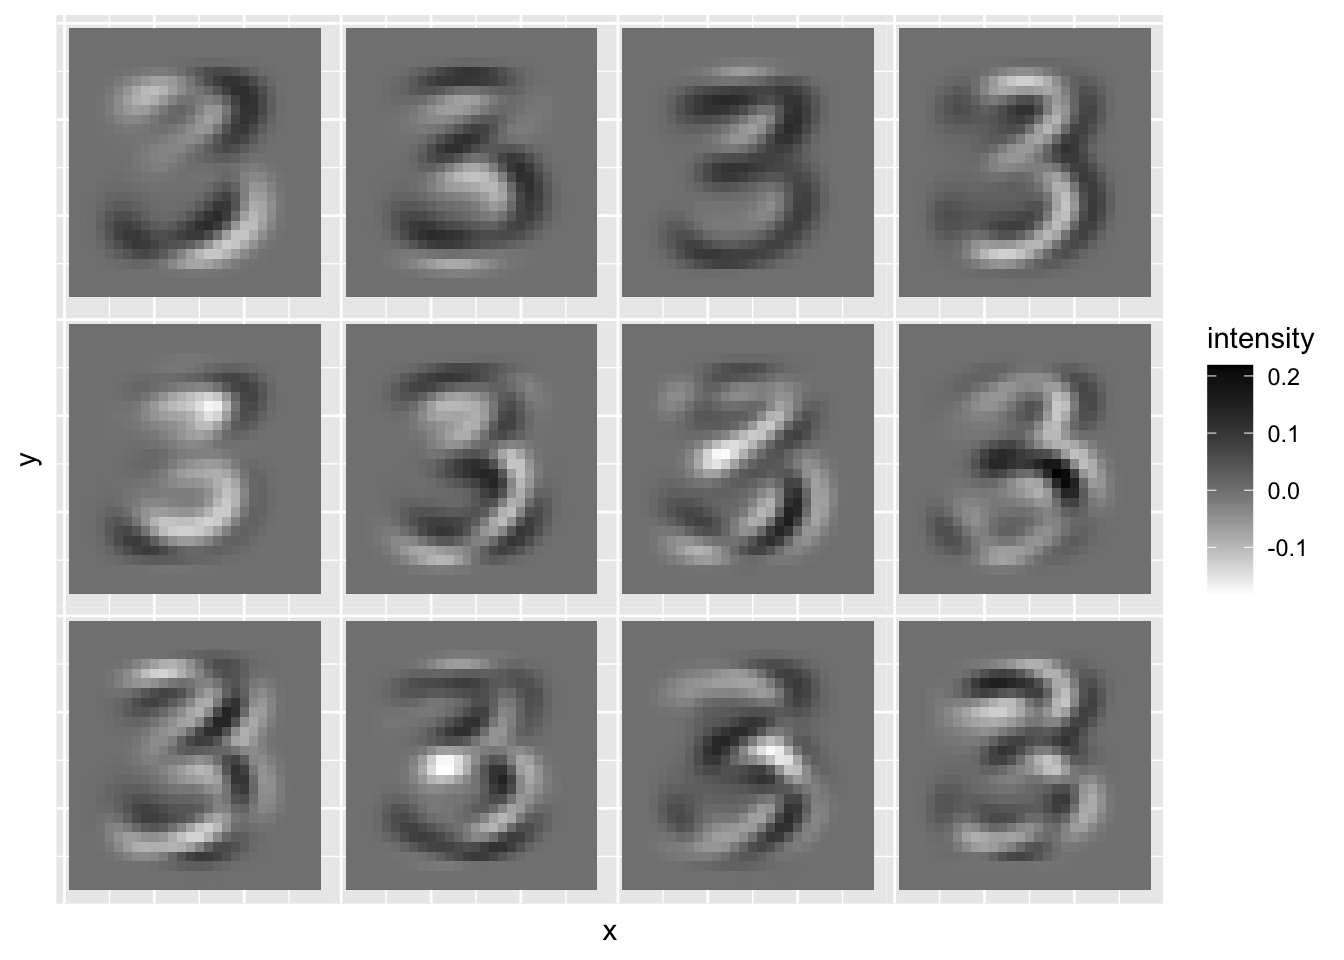
\includegraphics{04-pca_files/figure-latex/unnamed-chunk-33-1.pdf}

We can see there is quite a bit of variation between them.
Now lets look at \(\bar{\mathbf x}\), the average 3.

\begin{Shaded}
\begin{Highlighting}[]
\NormalTok{xbar=}\KeywordTok{colMeans}\NormalTok{(mnist3)}
\KeywordTok{plot.mnist}\NormalTok{(xbar)}
\end{Highlighting}
\end{Shaded}

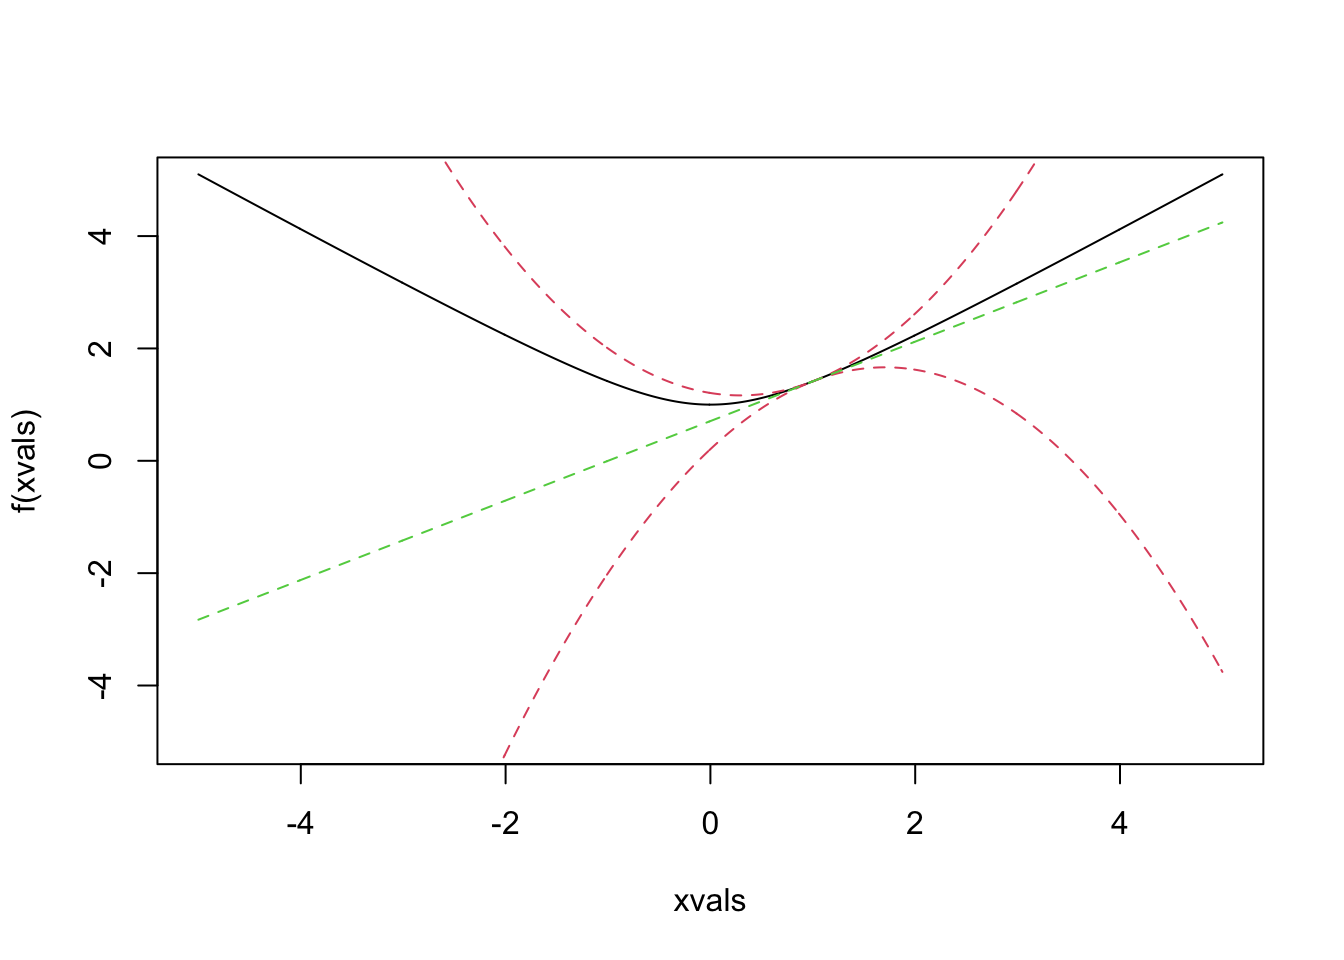
\includegraphics{04-pca_files/figure-latex/unnamed-chunk-34-1.pdf}

We can use the \texttt{prcomp} command to find the principal components. Note that we can't use the \texttt{scale=TRUE} option as some of the columns are all 0, and so R throws an error as it cannot rescale these to have variance 1. Let's plot the first few principal components/eigenvectors/loading vectors.

\begin{Shaded}
\begin{Highlighting}[]
\NormalTok{mnist3.pca <-}\StringTok{ }\KeywordTok{prcomp}\NormalTok{(mnist3)}
\KeywordTok{plot.mnist}\NormalTok{(mnist3.pca}\OperatorTok{$}\NormalTok{rotation[,}\DecValTok{1}\OperatorTok{:}\DecValTok{12}\NormalTok{]) }
\end{Highlighting}
\end{Shaded}

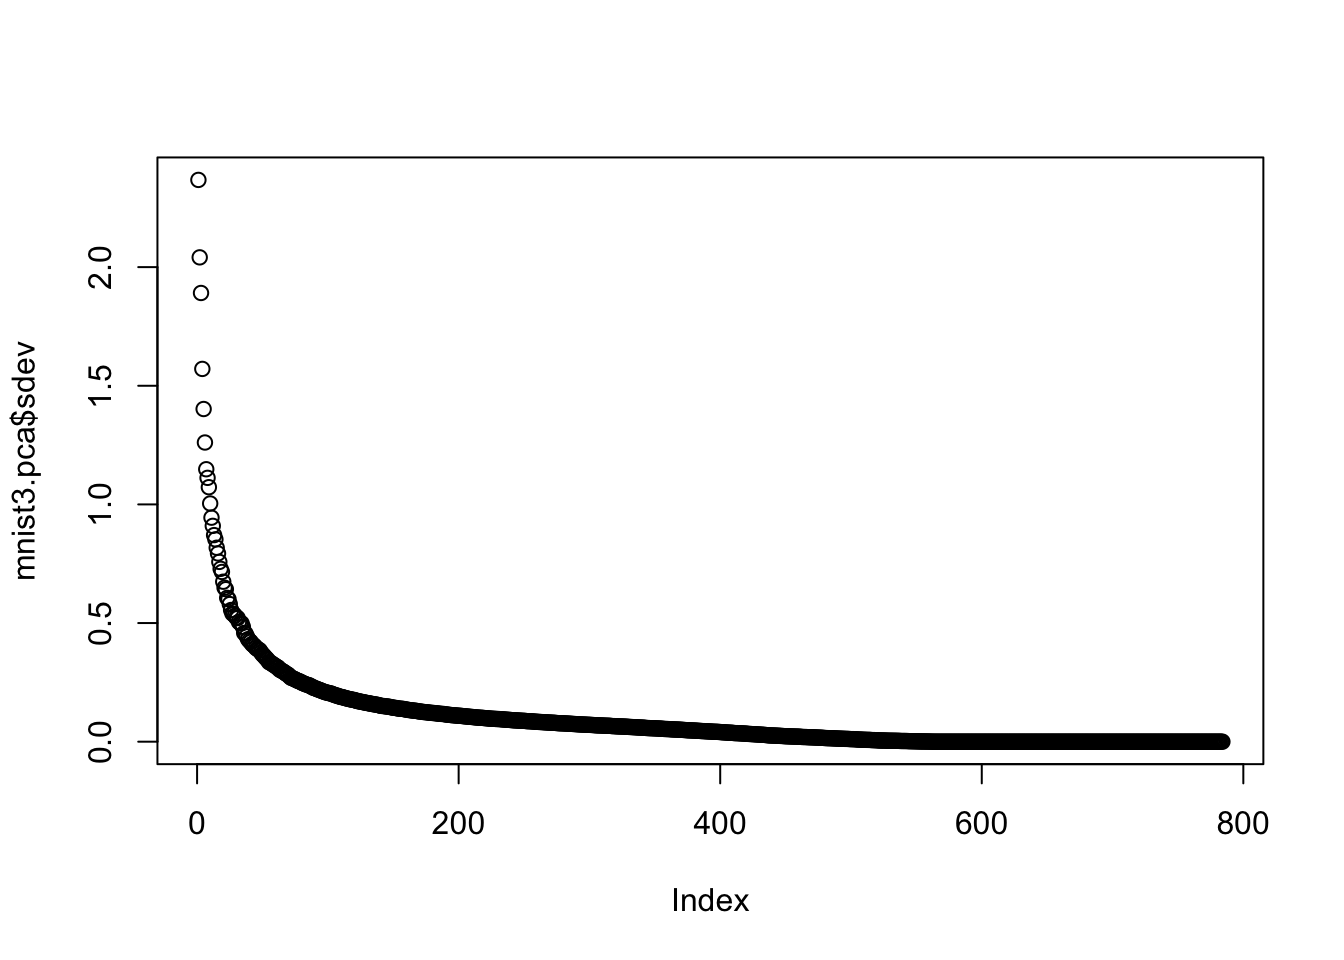
\includegraphics{04-pca_files/figure-latex/unnamed-chunk-35-1.pdf}

These show the main mode of variability in the 3s. Focusing on the first PC, we can see that this is a form of rotation and causes the 3 to slant either forward or backward. If we wanted a rank-2 approximation to the data we would use
\[f(\mathbf y) = \bar{\mathbf x} + y_1 \mathbf v_1 + y_2 \mathbf v_2\]

Let's try reconstructing the data with \(r=2\).

\begin{Shaded}
\begin{Highlighting}[]
\NormalTok{r=}\DecValTok{2}
\NormalTok{recon =}\StringTok{  }\NormalTok{mnist3.pca}\OperatorTok{$}\NormalTok{x[,}\DecValTok{1}\OperatorTok{:}\NormalTok{r] }\OperatorTok\StringTok{ }\KeywordTok{t}\NormalTok{(mnist3.pca}\OperatorTok{$}\NormalTok{rotation[,}\DecValTok{1}\OperatorTok{:}\NormalTok{r])}
\KeywordTok{plot.mnist2}\NormalTok{(}\KeywordTok{matrix}\NormalTok{(}\KeywordTok{rep}\NormalTok{(xbar,}\DecValTok{12}\NormalTok{), }\DataTypeTok{byrow=}\NormalTok{T, }\DataTypeTok{nr=}\DecValTok{12}\NormalTok{)}\OperatorTok{+}\NormalTok{recon[}\DecValTok{1}\OperatorTok{:}\DecValTok{12}\NormalTok{,])}
\end{Highlighting}
\end{Shaded}

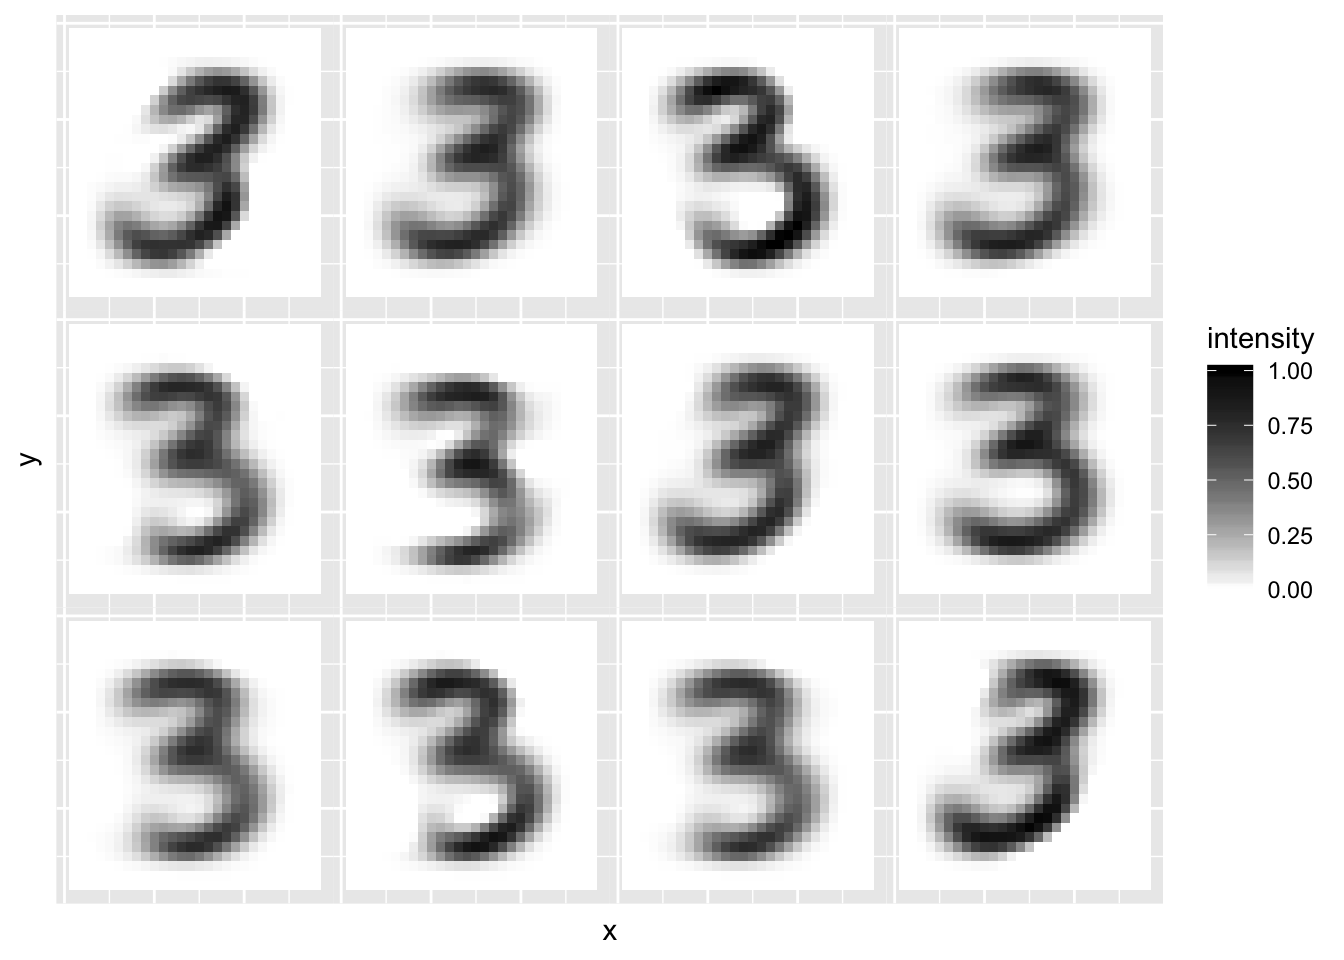
\includegraphics{04-pca_files/figure-latex/unnamed-chunk-36-1.pdf}

We can see that all of these 3s still look a lot like the average 3, but that they vary in their slant, and the heaviness of the line.

The scree plot shows a sharp decrease in the eigenvalues until about the 100th component, at which point they level off.

\begin{Shaded}
\begin{Highlighting}[]
\KeywordTok{plot}\NormalTok{(mnist3.pca}\OperatorTok{$}\NormalTok{sdev) }\CommentTok{# scree plot}
\end{Highlighting}
\end{Shaded}

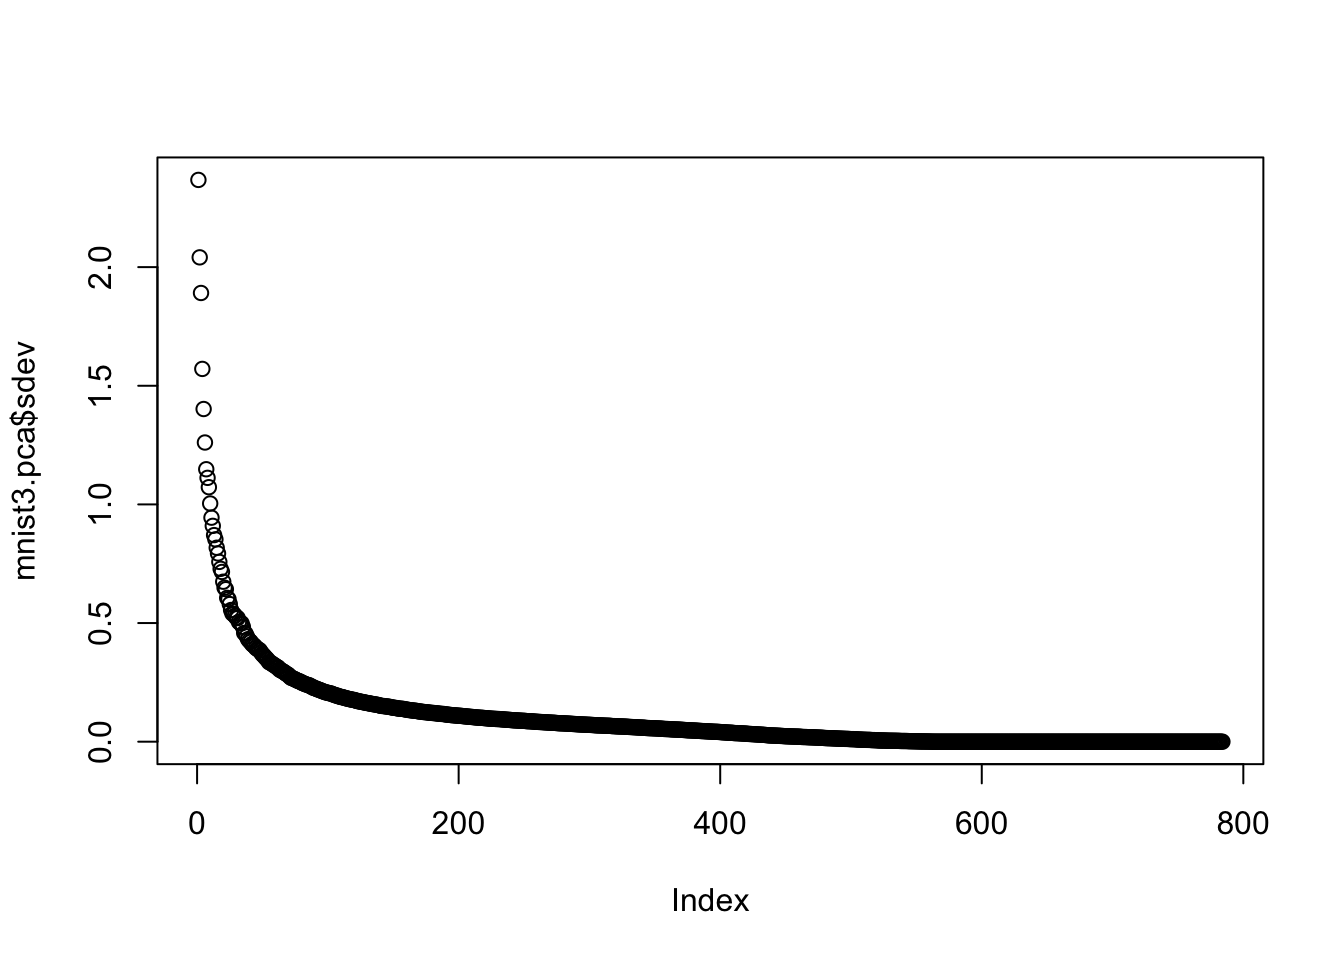
\includegraphics{04-pca_files/figure-latex/unnamed-chunk-37-1.pdf}

It can also be useful to plot the cumulative sum of the total proportion of variance explained by a given number of principal components. I've drawn on horizontal lines at 90\% and 95\% of variance explained, to help identify when we cross these thresholds.
We need 80 components to explain 90\% of the variance, and 138 components to explain 95\% of the variance.

\begin{Shaded}
\begin{Highlighting}[]
\NormalTok{cumvar =}\StringTok{ }\DecValTok{100}\OperatorTok{*}\KeywordTok{cumsum}\NormalTok{(mnist3.pca}\OperatorTok{$}\NormalTok{sdev}\OperatorTok{^}\DecValTok{2}\NormalTok{) }\OperatorTok{/}\StringTok{ }\KeywordTok{sum}\NormalTok{(mnist3.pca}\OperatorTok{$}\NormalTok{sdev}\OperatorTok{^}\DecValTok{2}\NormalTok{)}
\KeywordTok{plot}\NormalTok{(cumvar, }\DataTypeTok{ylab=}\StringTok{"Cumulative proportion of variance explained"}\NormalTok{, }\DataTypeTok{xlab=}\StringTok{"Number of PCs used"}\NormalTok{, }\DataTypeTok{ylim=}\KeywordTok{c}\NormalTok{(}\DecValTok{0}\NormalTok{,}\DecValTok{100}\NormalTok{))}
\KeywordTok{abline}\NormalTok{(}\DataTypeTok{h=}\DecValTok{90}\NormalTok{, }\DataTypeTok{lty=}\DecValTok{2}\NormalTok{)}
\KeywordTok{abline}\NormalTok{(}\DataTypeTok{v=}\KeywordTok{min}\NormalTok{(}\KeywordTok{which}\NormalTok{(cumvar}\OperatorTok{>}\DecValTok{90}\NormalTok{)), }\DataTypeTok{lty=}\DecValTok{2}\NormalTok{)}
\KeywordTok{abline}\NormalTok{(}\DataTypeTok{h=}\DecValTok{95}\NormalTok{, }\DataTypeTok{lty=}\DecValTok{2}\NormalTok{)}
\KeywordTok{abline}\NormalTok{(}\DataTypeTok{v=}\KeywordTok{min}\NormalTok{(}\KeywordTok{which}\NormalTok{(cumvar}\OperatorTok{>}\DecValTok{95}\NormalTok{)), }\DataTypeTok{lty=}\DecValTok{2}\NormalTok{)}
\end{Highlighting}
\end{Shaded}

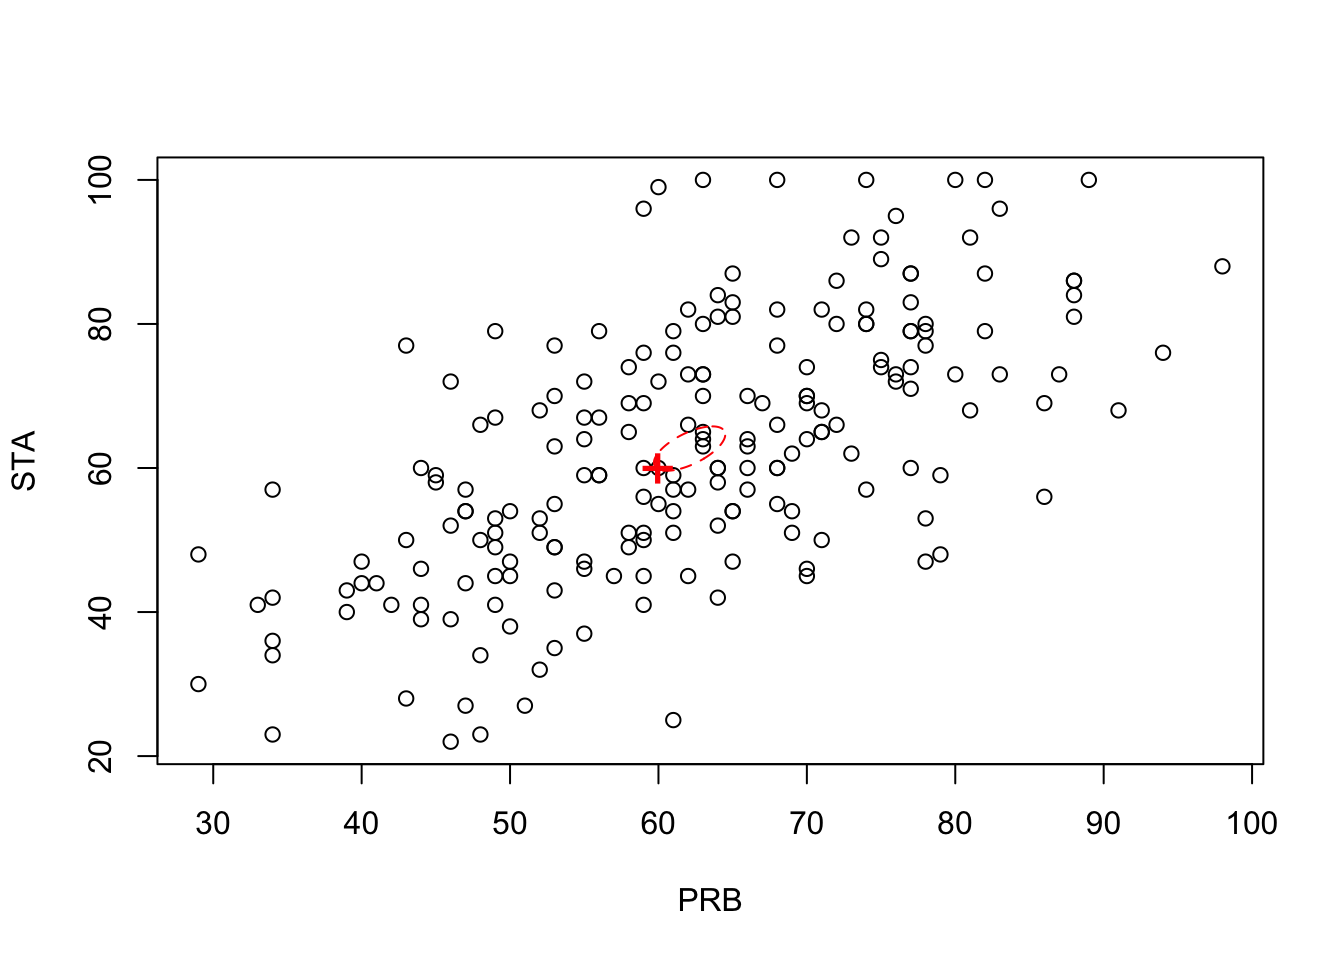
\includegraphics{04-pca_files/figure-latex/unnamed-chunk-39-1.pdf}

Let's now look at the reconstruction using \(r=10, \;50, \;100\) and \(500\) components to see how the accuracy changes.

\begin{Shaded}
\begin{Highlighting}[]
\NormalTok{r=}\DecValTok{10}
\NormalTok{recon =}\StringTok{  }\NormalTok{mnist3.pca}\OperatorTok{$}\NormalTok{x[,}\DecValTok{1}\OperatorTok{:}\NormalTok{r] }\OperatorTok\StringTok{ }\KeywordTok{t}\NormalTok{(mnist3.pca}\OperatorTok{$}\NormalTok{rotation[,}\DecValTok{1}\OperatorTok{:}\NormalTok{r])}
\KeywordTok{plot.mnist2}\NormalTok{(}\KeywordTok{matrix}\NormalTok{(}\KeywordTok{rep}\NormalTok{(xbar,}\DecValTok{12}\NormalTok{), }\DataTypeTok{byrow=}\NormalTok{T, }\DataTypeTok{nr=}\DecValTok{12}\NormalTok{)}\OperatorTok{+}\NormalTok{recon[}\DecValTok{1}\OperatorTok{:}\DecValTok{12}\NormalTok{,])}
\end{Highlighting}
\end{Shaded}

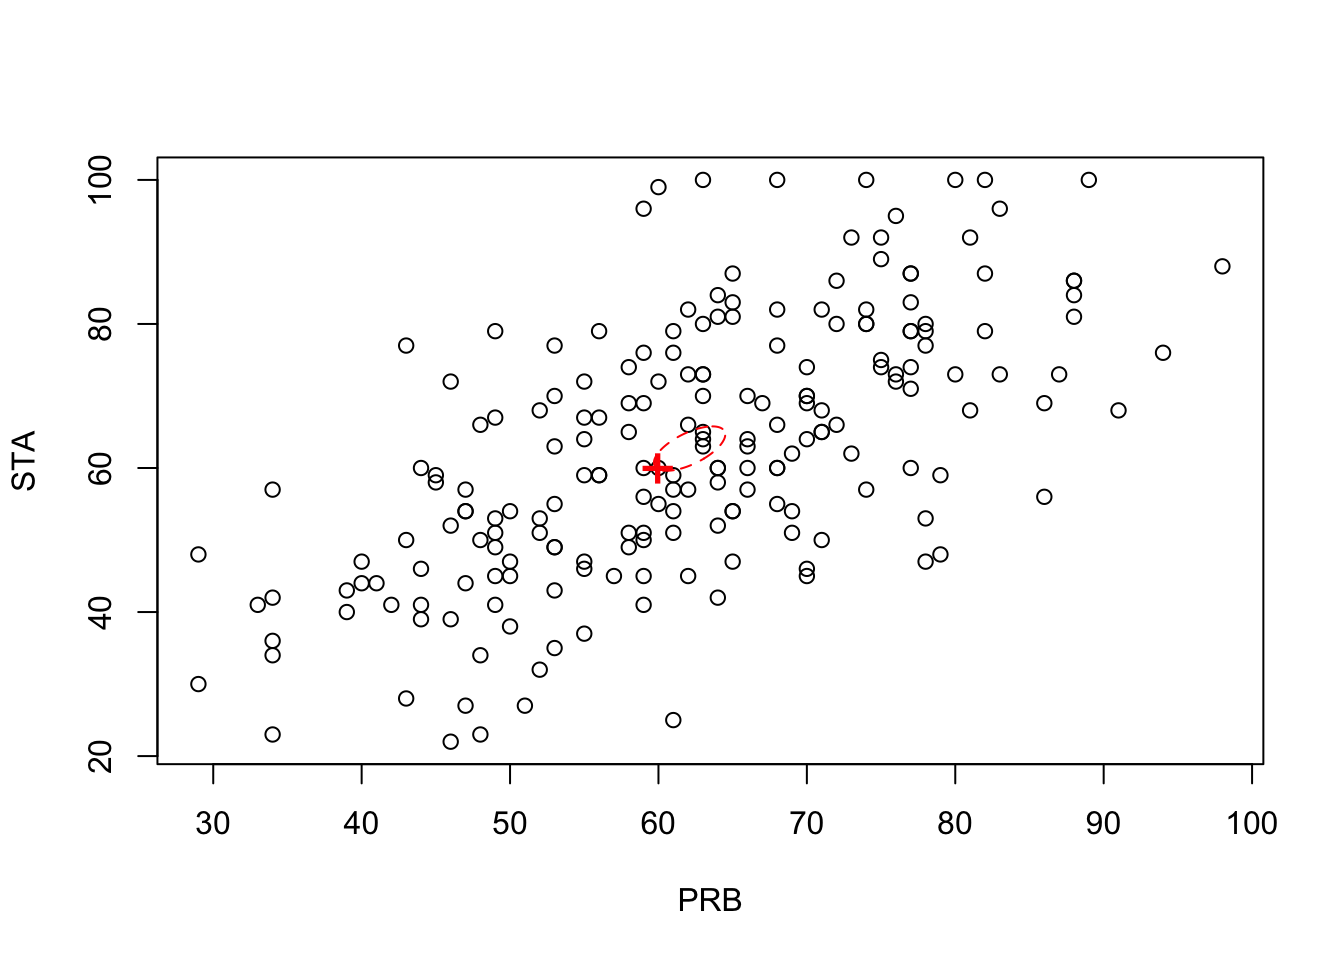
\includegraphics{04-pca_files/figure-latex/unnamed-chunk-40-1.pdf}

\begin{Shaded}
\begin{Highlighting}[]
\NormalTok{r=}\DecValTok{50}
\NormalTok{recon =}\StringTok{  }\NormalTok{mnist3.pca}\OperatorTok{$}\NormalTok{x[,}\DecValTok{1}\OperatorTok{:}\NormalTok{r] }\OperatorTok\StringTok{ }\KeywordTok{t}\NormalTok{(mnist3.pca}\OperatorTok{$}\NormalTok{rotation[,}\DecValTok{1}\OperatorTok{:}\NormalTok{r])}
\KeywordTok{plot.mnist2}\NormalTok{(}\KeywordTok{matrix}\NormalTok{(}\KeywordTok{rep}\NormalTok{(xbar,}\DecValTok{12}\NormalTok{), }\DataTypeTok{byrow=}\NormalTok{T, }\DataTypeTok{nr=}\DecValTok{12}\NormalTok{)}\OperatorTok{+}\NormalTok{recon[}\DecValTok{1}\OperatorTok{:}\DecValTok{12}\NormalTok{,])}
\end{Highlighting}
\end{Shaded}

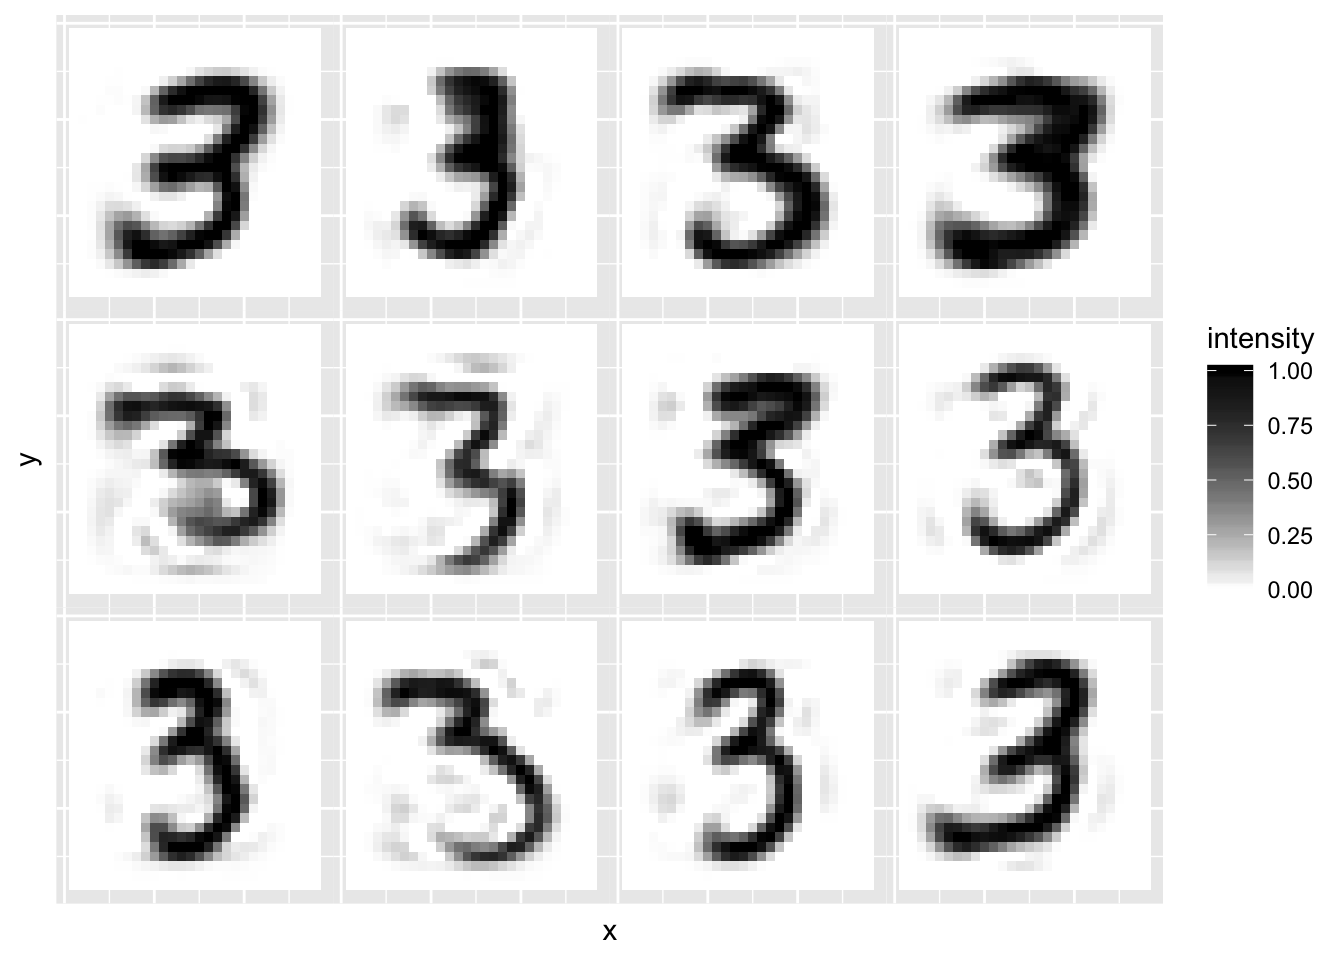
\includegraphics{04-pca_files/figure-latex/unnamed-chunk-41-1.pdf}

\begin{Shaded}
\begin{Highlighting}[]
\NormalTok{r=}\DecValTok{100}
\NormalTok{recon =}\StringTok{  }\NormalTok{mnist3.pca}\OperatorTok{$}\NormalTok{x[,}\DecValTok{1}\OperatorTok{:}\NormalTok{r] }\OperatorTok\StringTok{ }\KeywordTok{t}\NormalTok{(mnist3.pca}\OperatorTok{$}\NormalTok{rotation[,}\DecValTok{1}\OperatorTok{:}\NormalTok{r])}
\KeywordTok{plot.mnist2}\NormalTok{(}\KeywordTok{matrix}\NormalTok{(}\KeywordTok{rep}\NormalTok{(xbar,}\DecValTok{12}\NormalTok{), }\DataTypeTok{byrow=}\NormalTok{T, }\DataTypeTok{nr=}\DecValTok{12}\NormalTok{)}\OperatorTok{+}\NormalTok{recon[}\DecValTok{1}\OperatorTok{:}\DecValTok{12}\NormalTok{,])}
\end{Highlighting}
\end{Shaded}

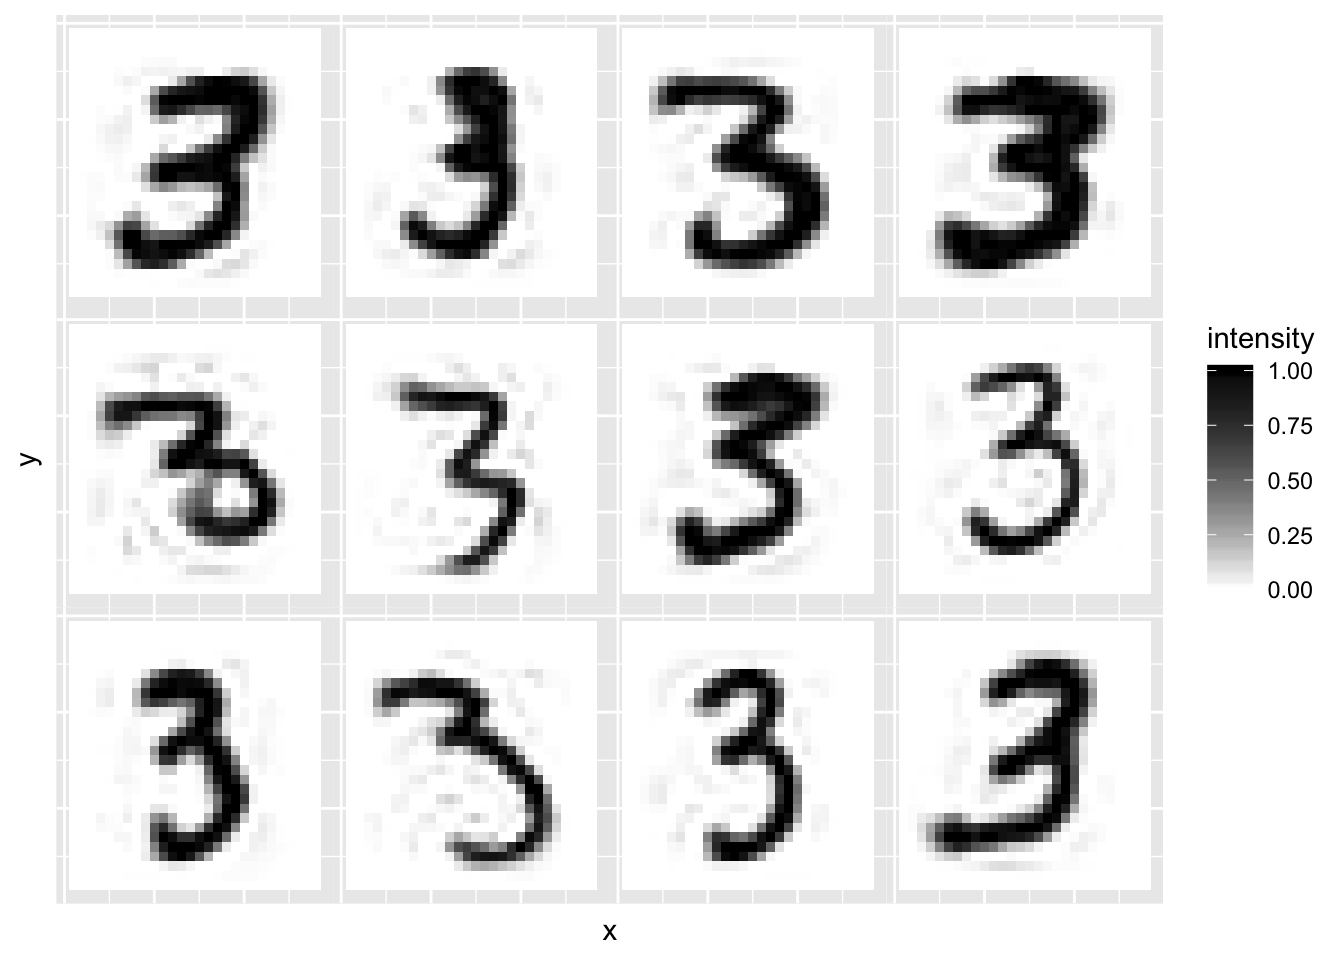
\includegraphics{04-pca_files/figure-latex/unnamed-chunk-42-1.pdf}

\begin{Shaded}
\begin{Highlighting}[]
\NormalTok{r=}\DecValTok{500}
\NormalTok{recon =}\StringTok{  }\NormalTok{mnist3.pca}\OperatorTok{$}\NormalTok{x[,}\DecValTok{1}\OperatorTok{:}\NormalTok{r] }\OperatorTok\StringTok{ }\KeywordTok{t}\NormalTok{(mnist3.pca}\OperatorTok{$}\NormalTok{rotation[,}\DecValTok{1}\OperatorTok{:}\NormalTok{r])}
\KeywordTok{plot.mnist2}\NormalTok{(}\KeywordTok{matrix}\NormalTok{(}\KeywordTok{rep}\NormalTok{(xbar,}\DecValTok{12}\NormalTok{), }\DataTypeTok{byrow=}\NormalTok{T, }\DataTypeTok{nr=}\DecValTok{12}\NormalTok{)}\OperatorTok{+}\NormalTok{recon[}\DecValTok{1}\OperatorTok{:}\DecValTok{12}\NormalTok{,])}
\end{Highlighting}
\end{Shaded}

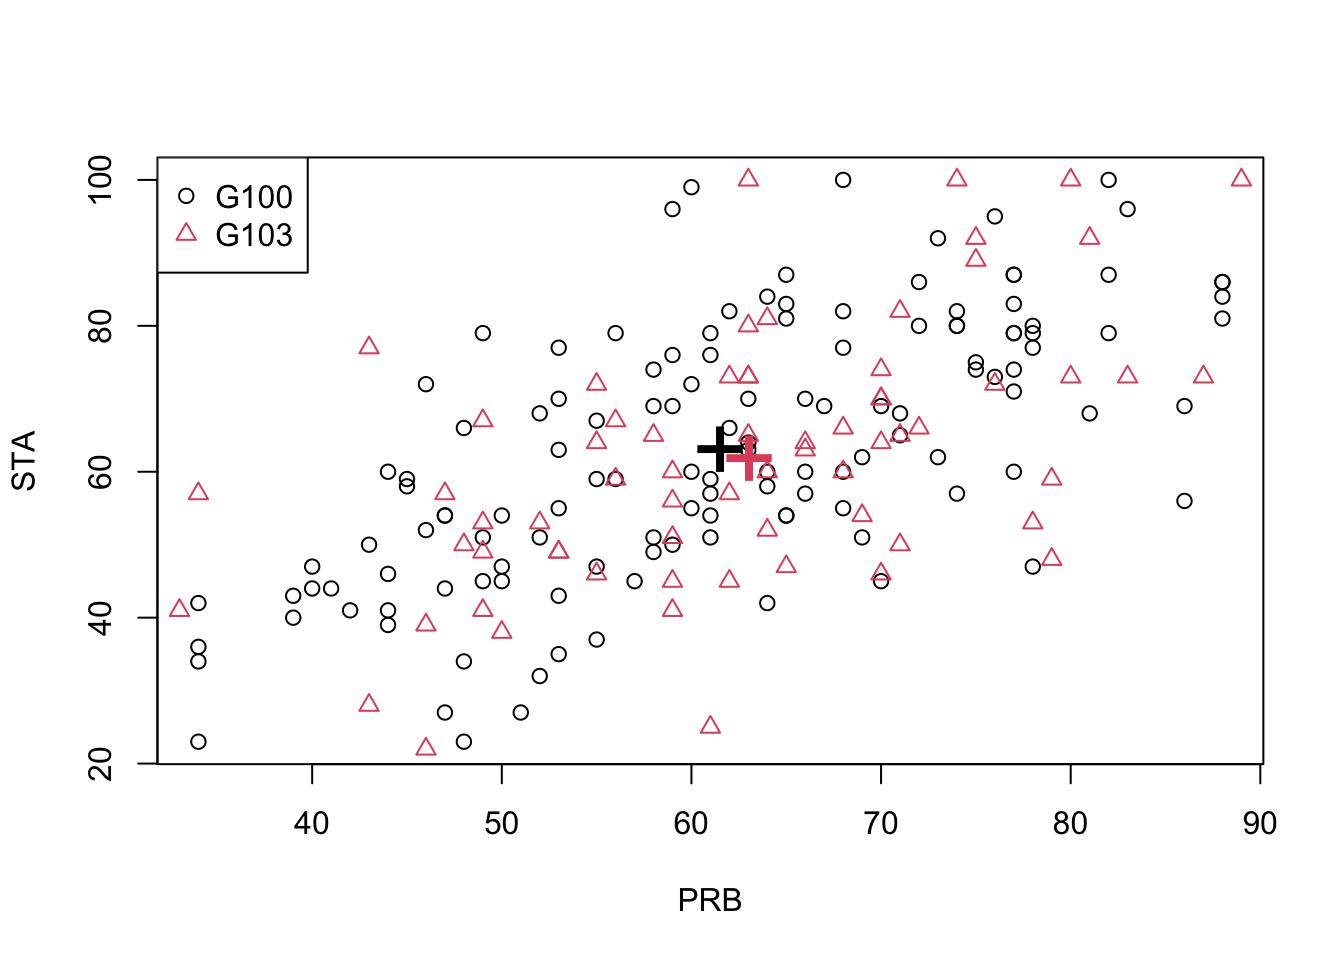
\includegraphics{04-pca_files/figure-latex/unnamed-chunk-43-1.pdf}

We can see that as the number of components increases the reconstructions start to look more like the original 12 images.

We can visualise the range of 3s by looking at a scatter plot of the first two principal components.

\begin{Shaded}
\begin{Highlighting}[]
\KeywordTok{library}\NormalTok{(ggplot2)}
\KeywordTok{qplot}\NormalTok{(mnist3.pca}\OperatorTok{$}\NormalTok{x[,}\DecValTok{1}\NormalTok{], mnist3.pca}\OperatorTok{$}\NormalTok{x[,}\DecValTok{2}\NormalTok{])}
\end{Highlighting}
\end{Shaded}

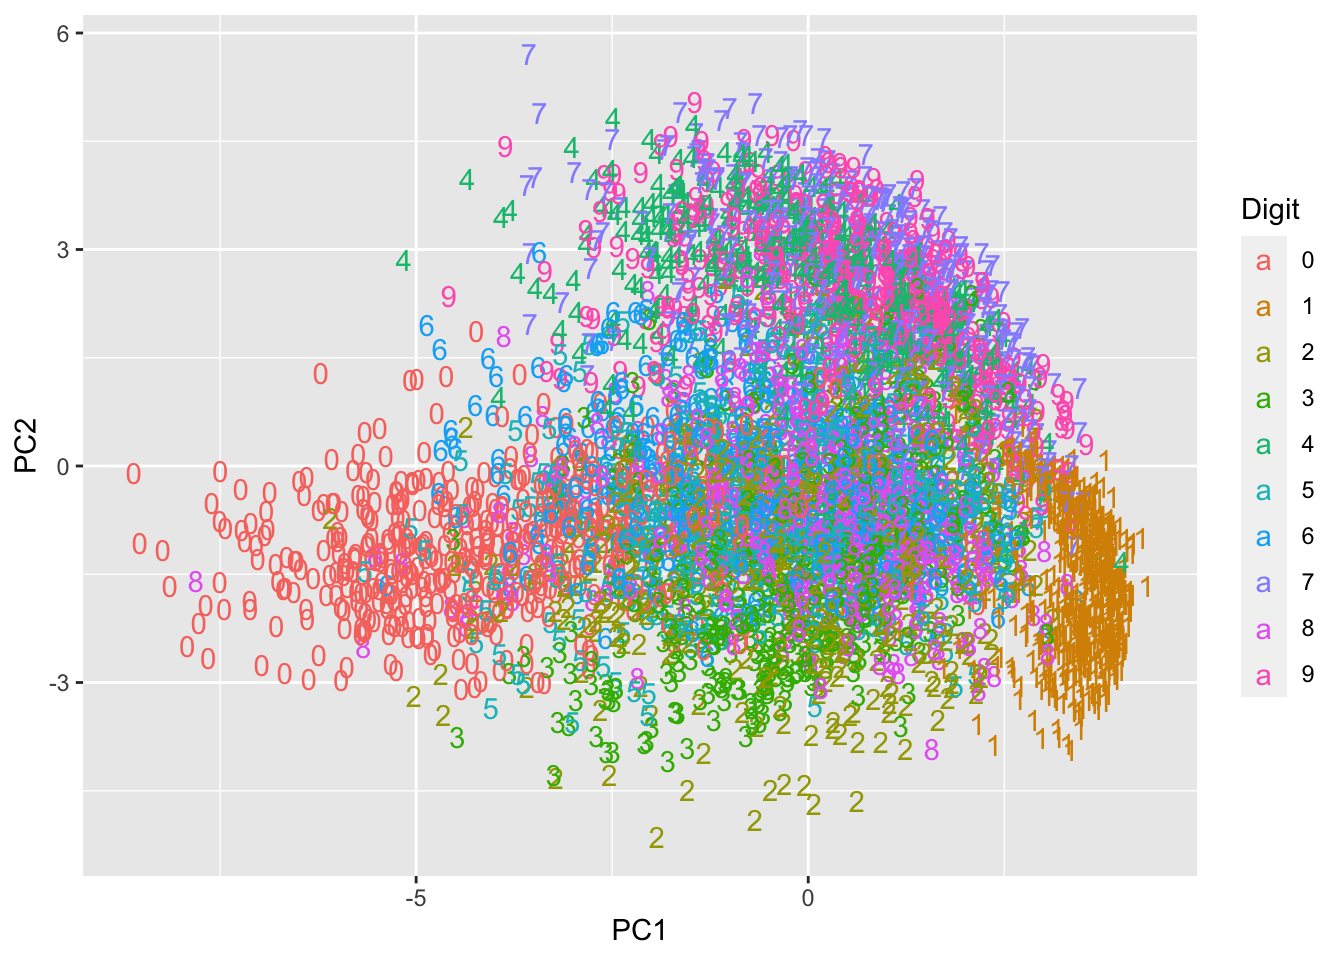
\includegraphics{04-pca_files/figure-latex/unnamed-chunk-44-1.pdf}

We can then finding images that differ according to these two PC scores. The first plot below is the 3 with the smallest PC1 score, and the second has the largest PC1 score. The third plot has the smallest PC2 score, and the fourth plot the largest PC2 score.
These four different 3s differ in more than just the first two principal components, but you can see the effect of the PC1 score is to slant the image forward or backward, whereas PC2 changes the thickness of the line.

\begin{Shaded}
\begin{Highlighting}[]
\NormalTok{image_list <-}\StringTok{ }\KeywordTok{c}\NormalTok{(}\KeywordTok{which.min}\NormalTok{(mnist3.pca}\OperatorTok{$}\NormalTok{x[,}\DecValTok{1}\NormalTok{]), }\KeywordTok{which.max}\NormalTok{(mnist3.pca}\OperatorTok{$}\NormalTok{x[,}\DecValTok{1}\NormalTok{]), }\KeywordTok{which.min}\NormalTok{(mnist3.pca}\OperatorTok{$}\NormalTok{x[,}\DecValTok{2}\NormalTok{]), }\KeywordTok{which.max}\NormalTok{(mnist3.pca}\OperatorTok{$}\NormalTok{x[,}\DecValTok{2}\NormalTok{]))}
\KeywordTok{plot.mnist}\NormalTok{(mnist3[image_list,]) }\CommentTok{# plot the first 12 images}
\end{Highlighting}
\end{Shaded}

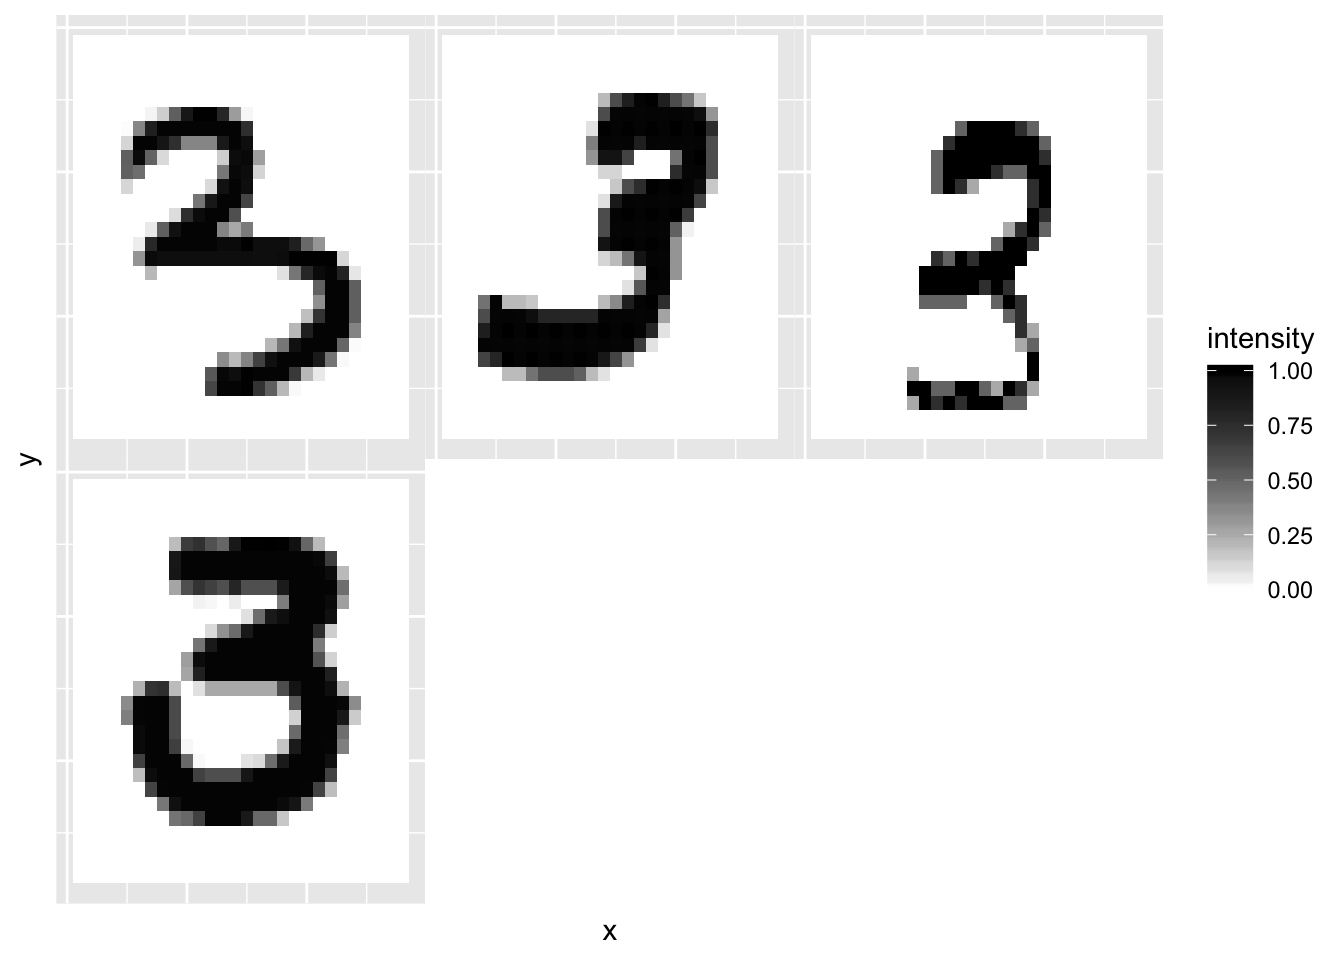
\includegraphics{04-pca_files/figure-latex/unnamed-chunk-45-1.pdf}

Finally, let's do PCA on a selection of the 60,000 images (not just the 3s). You can compute the SVD (which is what \texttt{prcomp} uses to do PCA) on a \(60,000 \times 784\) matrix, but it takes a long time on most computers, so here I've just computed the first two components on a random selection of 5,000 images using the option \texttt{rank=2} which significantly speeds up the computation time.

\begin{Shaded}
\begin{Highlighting}[]
\CommentTok{# Note this is slow to compute!}
\NormalTok{image_index <-}\StringTok{ }\KeywordTok{sample}\NormalTok{(}\DecValTok{1}\OperatorTok{:}\DecValTok{60000}\NormalTok{, }\DataTypeTok{size=}\DecValTok{5000}\NormalTok{) }\CommentTok{# select a random sample of images}
\NormalTok{mnist.pca <-}\StringTok{ }\KeywordTok{prcomp}\NormalTok{(mnist}\OperatorTok{$}\NormalTok{train}\OperatorTok{$}\NormalTok{x[image_index,], }\DataTypeTok{rank=}\DecValTok{2}\NormalTok{)}
\NormalTok{Digit =}\StringTok{ }\KeywordTok{as.factor}\NormalTok{(mnist}\OperatorTok{$}\NormalTok{train}\OperatorTok{$}\NormalTok{y[image_index])}
\KeywordTok{ggplot}\NormalTok{(}\KeywordTok{as.data.frame}\NormalTok{(mnist.pca}\OperatorTok{$}\NormalTok{x), }\KeywordTok{aes}\NormalTok{(}\DataTypeTok{x=}\NormalTok{PC1, }\DataTypeTok{y=}\NormalTok{PC2, }\DataTypeTok{colour=}\NormalTok{Digit, }\DataTypeTok{label=}\NormalTok{Digit))}\OperatorTok{+}
\KeywordTok{geom_text}\NormalTok{(}\KeywordTok{aes}\NormalTok{(}\DataTypeTok{label=}\NormalTok{Digit))}
\end{Highlighting}
\end{Shaded}

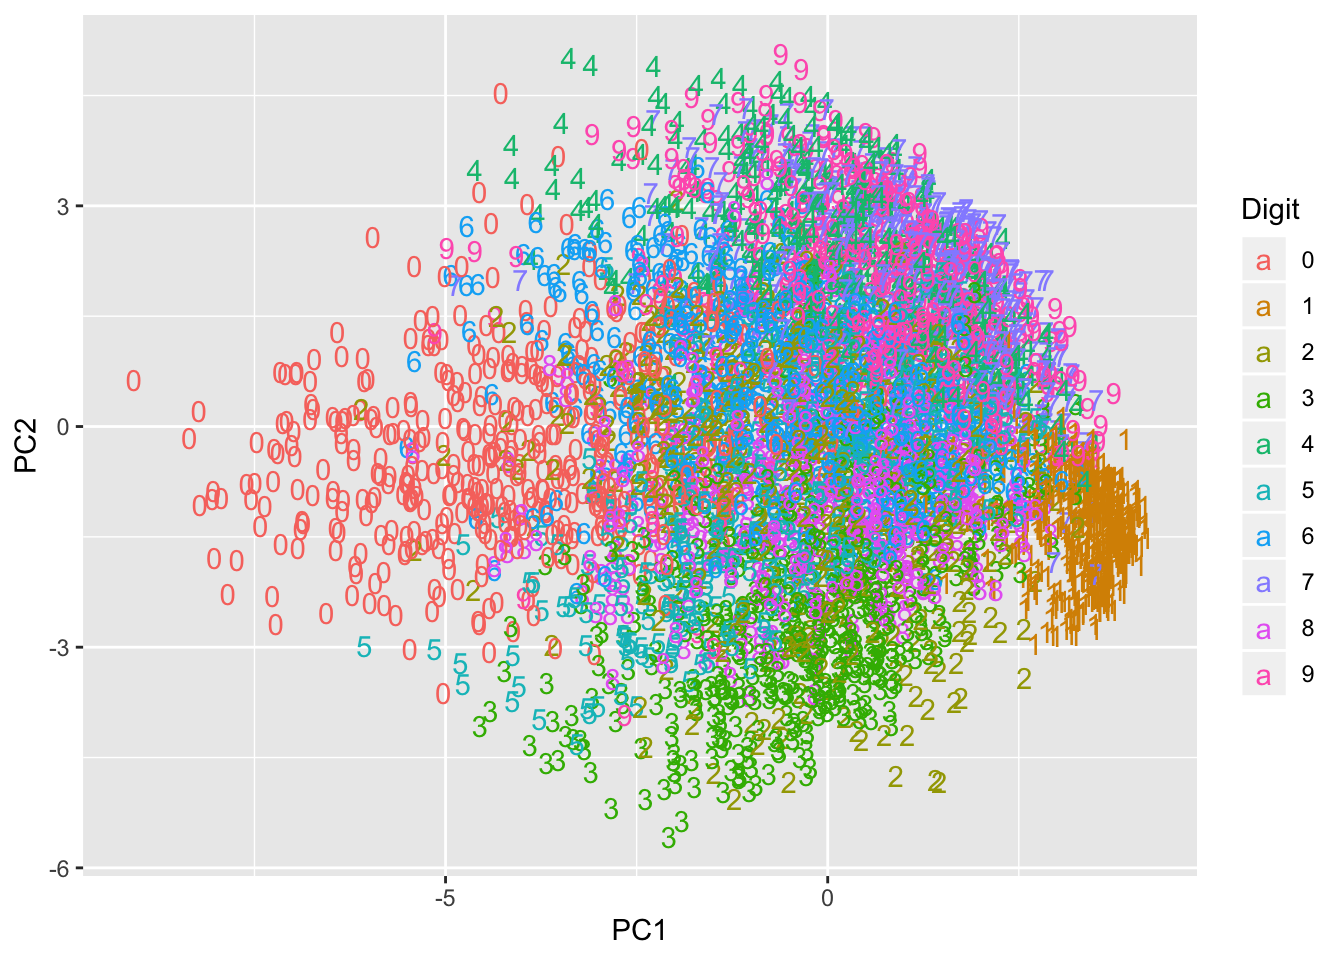
\includegraphics{04-pca_files/figure-latex/unnamed-chunk-46-1.pdf}

We can see from this scatter plot that the first two principal components do a surprisingly good job of separating and clustering the digits.

\hypertarget{pca-comptask}{%
\section{Computer tasks}\label{pca-comptask}}

\begin{enumerate}
\def\labelenumi{\arabic{enumi}.}
\item
  Using the \texttt{iris} dataset, familiarize yourself with the \texttt{prcomp} command and its output.

  Now, instead of using \texttt{prcomp} we will do the analysis ourselves using the \texttt{eigen} command.
\end{enumerate}

\begin{itemize}
\tightlist
\item
  Start by computing the sample mean and sample variance of the dataset (use \(n-1\) as the denominator when you compute the sample variance to get the same answer as provided by \texttt{prcomp}).
\item
  Now compute the eigenvalues and eigenvectors of the covariance matrix using \texttt{eigen}. Check that these agree with those computed by \texttt{prcomp} (noting that \texttt{prcomp} returns the standard deviation which is the square root of the eigenvalues).
\item
  Now compute the principal component scores by multiplying \(\mathbf X\) by the matrix of eigenvectors \(\mathbf V\). Check your answer agrees with the scores provided by \texttt{prcomp}.
\end{itemize}

Now we will do the same thing again, but using the \texttt{svd} command.

\begin{itemize}
\tightlist
\item
  Compute the column centred data matrix \(\frac{1}{\sqrt{n-1}}\mathbf H\mathbf X\)
\item
  Compute the SVD of this matrix. Check the singular values match the square root of the eigenvalues computed previously.
\item
  Compute the SVD scores by doing both \(\mathbf X\mathbf V\) and \(\mathbf U\boldsymbol{\Sigma}\).
\end{itemize}

\begin{enumerate}
\def\labelenumi{\arabic{enumi}.}
\setcounter{enumi}{1}
\tightlist
\item
  We first look at the crabs data, which is a dataset in the MASS library. First, we obtain the data.
  Then we focus on 5 continuous variables, all measured in mm: FL = frontal lobe size; RW = rear width; CL = carapace length;
  CW = carapace width; and BD = body depth. The sample size is \(200\).
\end{enumerate}

\begin{Shaded}
\begin{Highlighting}[]
\KeywordTok{library}\NormalTok{(MASS)}
\NormalTok{?crabs           }\CommentTok{# read the help page to find out about the dataset}
\NormalTok{X=crabs[}\DecValTok{4}\OperatorTok{:}\DecValTok{8}\NormalTok{]     }\CommentTok{# construct data matrix X with columns FL, RW, CL, CW, BD}
\end{Highlighting}
\end{Shaded}

Carry out PCA on the data in \(X\), including obtaining a scree plot and plotting the PC scores.

\begin{Shaded}
\begin{Highlighting}[]
\NormalTok{pca <-}\StringTok{ }\KeywordTok{prcomp}\NormalTok{(X, }\DataTypeTok{scale=}\OtherTok{FALSE}\NormalTok{)   }\CommentTok{#carry out PCA on S  }
\NormalTok{pca}
\NormalTok{lambda <-}\StringTok{ }\NormalTok{pca}\OperatorTok{$}\NormalTok{sdev}\OperatorTok{**}\DecValTok{2}    \CommentTok{#eigenvalues of S}
\KeywordTok{plot}\NormalTok{( lambda , }\DataTypeTok{ylim=}\KeywordTok{c}\NormalTok{( }\DecValTok{0}\NormalTok{, }\KeywordTok{max}\NormalTok{(lambda) )}
\KeywordTok{lines}\NormalTok{(lambda)}
\end{Highlighting}
\end{Shaded}

Some questions:

\begin{itemize}
\item
  Do you have any suggestions for an interpretation for the 1st PC?
\item
  Are you able to come up with an interpretation for the 2nd PC?
\item
  Do you think an analysis based on the sample covariance matrix \({\bf S}\) or the
  correlation matrix \({\bf R}\) is preferable with this dataset? Note that you can use \texttt{scale=TRUE} in \texttt{prcomp}
  to carry out PCA on \({\bf R}\). Does it make much difference which is used?
\item
  Without doing any computation, think about what you expect the sample mean and sample covariance matrix to be for the PC scores. Check this numerically.
\item
  Now check other properties of the PC scores listed in proposition \ref{prp:pca2}.
\item
  Try the following transformations of the data.

  \begin{itemize}
  \item
    adding a constant to the data
    \[\mathbf z= \mathbf x+\mathbf c,\]
  \item
    scaling the data:
    \[\mathbf z= \mathbf D\mathbf x\]
    for some diagonal matrix \(\mathbf D\)
  \item
    rotating the data:
    \[\mathbf z= \mathbf U\mathbf x\]
    for some \(p\times p\) orthogonal matrix \(\mathbf U\).
    You can generate a random orthogonal matrix using the following commands
  \end{itemize}
\end{itemize}

\begin{Shaded}
\begin{Highlighting}[]
\KeywordTok{library}\NormalTok{(pracma)}
\NormalTok{U <-}\StringTok{ }\KeywordTok{randortho}\NormalTok{(}\DecValTok{5}\NormalTok{)}
\end{Highlighting}
\end{Shaded}

Check the effect of each transformation on the principal components (the loadings/eigenvectors), the principal component scores, and the variance of the principal components (the eigenvalues).

\begin{enumerate}
\def\labelenumi{\arabic{enumi}.}
\setcounter{enumi}{2}
\tightlist
\item
  Download the final Premier League table for the 2018-19 season from
  \url{https://www.rotowire.com/soccer/league-table.php?season=2018}. There is a button to download the csv (comma separated variable) file in the bottom right hand corner.
\end{enumerate}

\begin{itemize}
\item
  Load the data into R using the command \texttt{read.csv}. Note that you may need to manually delete the first row of the csv file before doing this. (\emph{I haven't given you the command here, as learning how to do this yourself is important}).
\item
  Repeat the analysis from section \ref{pca:football}. Does the meaning of the principal components change? Was the 2018-19 league season notable different to the 2019-20 season (which is the season analysed in the notes)?
\end{itemize}

\hypertarget{exercises-1}{%
\section{Exercises}\label{exercises-1}}

\begin{enumerate}
\def\labelenumi{\arabic{enumi}.}
\tightlist
\item
  Consider the following data in \(\mathbb{R}^2\)
\end{enumerate}

\[\mathbf x_1 =\begin{pmatrix}1\\-1\end{pmatrix},\; \mathbf x_2 =\begin{pmatrix}-1\\1\end{pmatrix},
\;\mathbf x_3 =\begin{pmatrix}2\\2\end{pmatrix},\;\mathbf x_3 =\begin{pmatrix}-2\\-2\end{pmatrix}\]

\begin{itemize}
\item
  What is the orthogonal projection of these points onto \[\mathbf u_1 = \begin{pmatrix}1\\0\end{pmatrix}\] and onto \[\mathbf u_2 =\frac{1}{\sqrt{5}}\begin{pmatrix}1\\2\end{pmatrix}?\]
\item
  Compute the sample variance matrix of the three data points, and compute its spectral decomposition.
\item
  What vector \(\mathbf u\) would maximize the variance of these projection?
\item
  What vector \(\mathbf u\) would minimize
  \[\sum_{i=1}^4 ||\mathbf x_i -\mathbf u\mathbf u^\top \mathbf x_i||^2_2?\]
  This is the sum of squared errors from a rank 1 approximation to the data.
\item
  Plot the data points and convince yourself that your answers make intuitive sense.
\end{itemize}

\begin{enumerate}
\def\labelenumi{\arabic{enumi}.}
\setcounter{enumi}{1}
\tightlist
\item
  Consider a population covariance matrix \(\boldsymbol{\Sigma}\) of the form
  \[\boldsymbol{\Sigma}=\gamma \mathbf I_p + \mathbf a\mathbf a^\top\]
  where \(\gamma>0\) is a scalar, \(\mathbf I_p\) is the \(p \times p\) identity matrix and \(\mathbf a\) is a vector of dimension \(p\).

  \begin{itemize}
  \tightlist
  \item
    Show that \(\mathbf a\) is an eigenvector of \(\boldsymbol{\Sigma}\).
  \item
    Show that if \(\mathbf b\) is any vector such that \(\mathbf a^\top \mathbf b=0\), then \(\mathbf b\) is also an eigenvector of \(\boldsymbol{\Sigma}\).
  \item
    Obtain all the eigenvalues of \(\boldsymbol{\Sigma}\).
  \item
    Determine expressions for the proportion of variability `explained' by:
  \end{itemize}

  \begin{enumerate}
  \def\labelenumii{\roman{enumii}.}
  \tightlist
  \item
    the largest (population) principal component of \(\boldsymbol{\Sigma}\);
  \item
    the \(r\) largest (population) principal components of \(\boldsymbol{\Sigma}\), where \(1 < r \leq p\).
  \end{enumerate}
\item
  A covariance matrix has the following eigenvalues:
\end{enumerate}

\begin{verbatim}
##  [1] 4.22 2.38 1.88 1.11 0.91 0.82 0.58 0.44 0.35 0.19 0.05 0.04 0.04
\end{verbatim}

\begin{itemize}
\tightlist
\item
  Sketch a scree plot.
\item
  Determine the minimum number of principal components needed to explain 90\% of the total variation.
\item
  Determine the number of principal components whose eigenvalues are above average.
\end{itemize}

\begin{enumerate}
\def\labelenumi{\arabic{enumi}.}
\setcounter{enumi}{3}
\item
  Measurements are taken on \(p=3\) variables \(x_1\), \(x_2\) and \(x_3\), with sample correlation matrix
  \[
   \mathbf R= \begin{pmatrix} 1 & 0.5792 & 0.2414 \\ 0.5792 & 1 & 0.5816 \\ 0.2414 & 0.5816 & 1 \end{pmatrix}.
  \]
  The variable \(z_j\) is the standardised versions of \(x_j\), \(j=1,2,3\), i.e.~each \(z_j\) has sample mean \(0\) and variance \(1\).
  One observation has \(z_1 = z_2 = z_3 = 0\) and a second observation has \(z_1 = z_2 = z_3 =1\). Calculate the three
  principal component scores for
  each of these observations.
\item
  Do exam question 1 part (a) from the 2017-18 exam paper. You will find the past exam papers on Moodle.
\end{enumerate}

\bibliography{book.bib,packages.bib}

\end{document}
